% Options for packages loaded elsewhere
\PassOptionsToPackage{unicode}{hyperref}
\PassOptionsToPackage{hyphens}{url}
%
\documentclass[
]{article}
\usepackage{amsmath,amssymb}
\usepackage{lmodern}
\usepackage{iftex}
\ifPDFTeX
  \usepackage[T1]{fontenc}
  \usepackage[utf8]{inputenc}
  \usepackage{textcomp} % provide euro and other symbols
\else % if luatex or xetex
  \usepackage{unicode-math}
  \defaultfontfeatures{Scale=MatchLowercase}
  \defaultfontfeatures[\rmfamily]{Ligatures=TeX,Scale=1}
\fi
% Use upquote if available, for straight quotes in verbatim environments
\IfFileExists{upquote.sty}{\usepackage{upquote}}{}
\IfFileExists{microtype.sty}{% use microtype if available
  \usepackage[]{microtype}
  \UseMicrotypeSet[protrusion]{basicmath} % disable protrusion for tt fonts
}{}
\makeatletter
\@ifundefined{KOMAClassName}{% if non-KOMA class
  \IfFileExists{parskip.sty}{%
    \usepackage{parskip}
  }{% else
    \setlength{\parindent}{0pt}
    \setlength{\parskip}{6pt plus 2pt minus 1pt}}
}{% if KOMA class
  \KOMAoptions{parskip=half}}
\makeatother
\usepackage{xcolor}
\usepackage[margin=1in]{geometry}
\usepackage{color}
\usepackage{fancyvrb}
\newcommand{\VerbBar}{|}
\newcommand{\VERB}{\Verb[commandchars=\\\{\}]}
\DefineVerbatimEnvironment{Highlighting}{Verbatim}{commandchars=\\\{\}}
% Add ',fontsize=\small' for more characters per line
\usepackage{framed}
\definecolor{shadecolor}{RGB}{248,248,248}
\newenvironment{Shaded}{\begin{snugshade}}{\end{snugshade}}
\newcommand{\AlertTok}[1]{\textcolor[rgb]{0.94,0.16,0.16}{#1}}
\newcommand{\AnnotationTok}[1]{\textcolor[rgb]{0.56,0.35,0.01}{\textbf{\textit{#1}}}}
\newcommand{\AttributeTok}[1]{\textcolor[rgb]{0.77,0.63,0.00}{#1}}
\newcommand{\BaseNTok}[1]{\textcolor[rgb]{0.00,0.00,0.81}{#1}}
\newcommand{\BuiltInTok}[1]{#1}
\newcommand{\CharTok}[1]{\textcolor[rgb]{0.31,0.60,0.02}{#1}}
\newcommand{\CommentTok}[1]{\textcolor[rgb]{0.56,0.35,0.01}{\textit{#1}}}
\newcommand{\CommentVarTok}[1]{\textcolor[rgb]{0.56,0.35,0.01}{\textbf{\textit{#1}}}}
\newcommand{\ConstantTok}[1]{\textcolor[rgb]{0.00,0.00,0.00}{#1}}
\newcommand{\ControlFlowTok}[1]{\textcolor[rgb]{0.13,0.29,0.53}{\textbf{#1}}}
\newcommand{\DataTypeTok}[1]{\textcolor[rgb]{0.13,0.29,0.53}{#1}}
\newcommand{\DecValTok}[1]{\textcolor[rgb]{0.00,0.00,0.81}{#1}}
\newcommand{\DocumentationTok}[1]{\textcolor[rgb]{0.56,0.35,0.01}{\textbf{\textit{#1}}}}
\newcommand{\ErrorTok}[1]{\textcolor[rgb]{0.64,0.00,0.00}{\textbf{#1}}}
\newcommand{\ExtensionTok}[1]{#1}
\newcommand{\FloatTok}[1]{\textcolor[rgb]{0.00,0.00,0.81}{#1}}
\newcommand{\FunctionTok}[1]{\textcolor[rgb]{0.00,0.00,0.00}{#1}}
\newcommand{\ImportTok}[1]{#1}
\newcommand{\InformationTok}[1]{\textcolor[rgb]{0.56,0.35,0.01}{\textbf{\textit{#1}}}}
\newcommand{\KeywordTok}[1]{\textcolor[rgb]{0.13,0.29,0.53}{\textbf{#1}}}
\newcommand{\NormalTok}[1]{#1}
\newcommand{\OperatorTok}[1]{\textcolor[rgb]{0.81,0.36,0.00}{\textbf{#1}}}
\newcommand{\OtherTok}[1]{\textcolor[rgb]{0.56,0.35,0.01}{#1}}
\newcommand{\PreprocessorTok}[1]{\textcolor[rgb]{0.56,0.35,0.01}{\textit{#1}}}
\newcommand{\RegionMarkerTok}[1]{#1}
\newcommand{\SpecialCharTok}[1]{\textcolor[rgb]{0.00,0.00,0.00}{#1}}
\newcommand{\SpecialStringTok}[1]{\textcolor[rgb]{0.31,0.60,0.02}{#1}}
\newcommand{\StringTok}[1]{\textcolor[rgb]{0.31,0.60,0.02}{#1}}
\newcommand{\VariableTok}[1]{\textcolor[rgb]{0.00,0.00,0.00}{#1}}
\newcommand{\VerbatimStringTok}[1]{\textcolor[rgb]{0.31,0.60,0.02}{#1}}
\newcommand{\WarningTok}[1]{\textcolor[rgb]{0.56,0.35,0.01}{\textbf{\textit{#1}}}}
\usepackage{longtable,booktabs,array}
\usepackage{calc} % for calculating minipage widths
% Correct order of tables after \paragraph or \subparagraph
\usepackage{etoolbox}
\makeatletter
\patchcmd\longtable{\par}{\if@noskipsec\mbox{}\fi\par}{}{}
\makeatother
% Allow footnotes in longtable head/foot
\IfFileExists{footnotehyper.sty}{\usepackage{footnotehyper}}{\usepackage{footnote}}
\makesavenoteenv{longtable}
\usepackage{graphicx}
\makeatletter
\def\maxwidth{\ifdim\Gin@nat@width>\linewidth\linewidth\else\Gin@nat@width\fi}
\def\maxheight{\ifdim\Gin@nat@height>\textheight\textheight\else\Gin@nat@height\fi}
\makeatother
% Scale images if necessary, so that they will not overflow the page
% margins by default, and it is still possible to overwrite the defaults
% using explicit options in \includegraphics[width, height, ...]{}
\setkeys{Gin}{width=\maxwidth,height=\maxheight,keepaspectratio}
% Set default figure placement to htbp
\makeatletter
\def\fps@figure{htbp}
\makeatother
\setlength{\emergencystretch}{3em} % prevent overfull lines
\providecommand{\tightlist}{%
  \setlength{\itemsep}{0pt}\setlength{\parskip}{0pt}}
\setcounter{secnumdepth}{-\maxdimen} % remove section numbering
\ifLuaTeX
  \usepackage{selnolig}  % disable illegal ligatures
\fi
\IfFileExists{bookmark.sty}{\usepackage{bookmark}}{\usepackage{hyperref}}
\IfFileExists{xurl.sty}{\usepackage{xurl}}{} % add URL line breaks if available
\urlstyle{same} % disable monospaced font for URLs
\hypersetup{
  pdftitle={Posit Primers},
  hidelinks,
  pdfcreator={LaTeX via pandoc}}

\title{Posit Primers}
\author{}
\date{\vspace{-2.5em}}

\begin{document}
\maketitle

{
\setcounter{tocdepth}{2}
\tableofcontents
}
Last Updated: 2023-01-14

URL \url{https://rstudio.cloud/learn/primers}

GitHUb: \url{https://github.com/rstudio-education/primers}

\begin{quote}
These interactive tutorials were all created using the learnr package.
If you would like to learn how to create your own tutorials, visit the
learnr site at \url{https://rstudio.github.io/learnr/}.
\end{quote}

\hypertarget{the-basics}{%
\section{The Basics}\label{the-basics}}

Start here to learn the skills that you will rely on in every analysis
(and every primer that follows): how to inspect, visualize, subset, and
transform your data, as well as how to run code.

If you're ready to begin, go to the first tutorial. There is no need to
install or download anything. Each tutorial has everything you need to
write and run R code, right in the tutorial.

\hypertarget{data-visualization-basics}{%
\subsection{Data Visualization Basics}\label{data-visualization-basics}}

Start here and begin making plots with R. Plots are one of the most
important tools for data science; they are also one of the most fun.

\hypertarget{welcome}{%
\subsubsection{Welcome}\label{welcome}}

Visualization is one of the most important tools for data science.

It is also a great way to start learning R; when you visualize data, you
get an immediate payoff that will keep you motivated as you learn.
Afterall, learning a new language can be hard!

This tutorial will teach you how to visualize data with R's most popular
visualization package, \texttt{ggplot2}.

The tutorial focuses on three basic skills:

\begin{enumerate}
\def\labelenumi{\arabic{enumi}.}
\tightlist
\item
  How to create graphs with a reusable \textbf{template}
\item
  How to add variables to a graph with \textbf{aesthetics}
\item
  How to make different ``types'' of graphs with \textbf{geoms}
\end{enumerate}

In this tutorial, we will use the \href{http://tidyverse.org/}{core
tidyverse packages}, including ggplot2. I've already loaded the packages
for you, so let's begin!

These examples are excerpted from \href{https://r4ds.had.co.nz}{R for
Data Science} by Hadley Wickham and Garrett Grolemund, published by
O'Reilly Media, Inc., 2016, ISBN: 9781491910399. You can purchase the
book at shop.oreilly.com.

\hypertarget{a-code-template}{%
\subsubsection{A code template}\label{a-code-template}}

\begin{quote}
``The simple graph has brought more information to the data analyst's
mind than any other device.'' --- John Tukey
\end{quote}

Let's begin with a question to explore.

\textbf{What do you think: Do cars with bigger engines use more fuel
than cars with smaller engines?}

\begin{itemize}
\tightlist
\item[$\boxtimes$]
  Cars with bigger engines use more fuel. ✓
\item[$\square$]
  Cars with bigger engines use less fuel. ✓
\end{itemize}

\begin{verbatim}
Great! 

In other words, there is a positive relationship between engine size and fuel efficiency. Now let's test your hypothesis against data.
\end{verbatim}

\hypertarget{mpg}{%
\paragraph{\texorpdfstring{\texttt{mpg}}{mpg}}\label{mpg}}

You can test your hypothesis with the mpg dataset that comes in the
ggplot2 package. mpg contains observations collected on 38 models of
cars by the US Environmental Protection Agency.

To see the mpg data frame, type mpg in the code block below and click
``Submit Answer''.

\begin{Shaded}
\begin{Highlighting}[]
\CommentTok{\# mpg is a data in the ggplot2 package. So required to load ggplot2 which is in tidyverse.}
\FunctionTok{library}\NormalTok{(tidyverse)}
\end{Highlighting}
\end{Shaded}

\begin{verbatim}
## -- Attaching packages --------------------------------------- tidyverse 1.3.2 --
## v ggplot2 3.4.0      v purrr   1.0.0 
## v tibble  3.1.8      v dplyr   1.0.10
## v tidyr   1.2.1      v stringr 1.5.0 
## v readr   2.1.3      v forcats 0.5.2 
## -- Conflicts ------------------------------------------ tidyverse_conflicts() --
## x dplyr::filter() masks stats::filter()
## x dplyr::lag()    masks stats::lag()
\end{verbatim}

\begin{Shaded}
\begin{Highlighting}[]
\NormalTok{mpg}
\end{Highlighting}
\end{Shaded}

\begin{verbatim}
## # A tibble: 234 x 11
##    manufacturer model      displ  year   cyl trans drv     cty   hwy fl    class
##    <chr>        <chr>      <dbl> <int> <int> <chr> <chr> <int> <int> <chr> <chr>
##  1 audi         a4           1.8  1999     4 auto~ f        18    29 p     comp~
##  2 audi         a4           1.8  1999     4 manu~ f        21    29 p     comp~
##  3 audi         a4           2    2008     4 manu~ f        20    31 p     comp~
##  4 audi         a4           2    2008     4 auto~ f        21    30 p     comp~
##  5 audi         a4           2.8  1999     6 auto~ f        16    26 p     comp~
##  6 audi         a4           2.8  1999     6 manu~ f        18    26 p     comp~
##  7 audi         a4           3.1  2008     6 auto~ f        18    27 p     comp~
##  8 audi         a4 quattro   1.8  1999     4 manu~ 4        18    26 p     comp~
##  9 audi         a4 quattro   1.8  1999     4 auto~ 4        16    25 p     comp~
## 10 audi         a4 quattro   2    2008     4 manu~ 4        20    28 p     comp~
## # ... with 224 more rows
\end{verbatim}

\begin{verbatim}
"Good job! We'll use interactive code chunks like this throughout these tutorials. 
Whenever you encounter one, you can click Submit Answer to run (or re-run) the code in the chunk. 
If there is a Solution button, you can click it to see the answer."
\end{verbatim}

You can use the black triangle that appears at the top right of the
table to scroll through all of the columns in mpg.

Among the variables in mpg are:

\begin{enumerate}
\def\labelenumi{\arabic{enumi}.}
\tightlist
\item
  displ, a car's engine size, in liters.
\item
  hwy, a car's fuel efficiency on the highway, in miles per gallon
  (mpg). A car with a low mpg consumes more fuel than a car with a high
  mpg when they travel the same distance.
\end{enumerate}

Now let's use this data to make our first graph.

\hypertarget{a-plot}{%
\paragraph{A plot}\label{a-plot}}

The code below uses functions from the ggplot2 package to plot the
relationship between displ and hwy.

To see the plot, click ``Run Code.''

\begin{Shaded}
\begin{Highlighting}[]
\FunctionTok{ggplot}\NormalTok{(}\AttributeTok{data =}\NormalTok{ mpg) }\SpecialCharTok{+} 
  \FunctionTok{geom\_point}\NormalTok{(}\AttributeTok{mapping =} \FunctionTok{aes}\NormalTok{(}\AttributeTok{x =}\NormalTok{ displ, }\AttributeTok{y =}\NormalTok{ hwy))}
\end{Highlighting}
\end{Shaded}

\includegraphics{rstudio_primers_files/figure-latex/unnamed-chunk-3-1.pdf}

Can you spot the relationship?

\hypertarget{and-the-answer-is}{%
\paragraph{And the answer is\ldots{}}\label{and-the-answer-is}}

The plot shows a negative relationship between engine size (displ) and
fuel efficiency (hwy). Points that have a large value of displ have a
small value of hwy and vice versa.

In other words, cars with big engines use more fuel. If that was your
hypothesis, you were right!

Now let's look at how we made the plot.

\hypertarget{ggplot}{%
\paragraph{\texorpdfstring{\texttt{ggplot}()}{ggplot()}}\label{ggplot}}

Here's the code that we used to make the plot. Notice that it contains
three functions: ggplot(), geom\_point(), and aes().

\begin{verbatim}
ggplot(data = mpg) + 
  geom_point(mapping = aes(x = displ, y = hwy))
\end{verbatim}

In R, a function is a name followed by a set of parentheses. Many
functions require special information to do their jobs, and you write
this information between the parentheses.

\hypertarget{ggplot-1}{%
\paragraph{ggplot}\label{ggplot-1}}

The first function, ggplot(), creates a coordinate system that you can
add layers to. The first argument of ggplot() is the dataset to use in
the graph.

By itself, ggplot(data = mpg) creates an empty graph, which looks like
this.

\begin{Shaded}
\begin{Highlighting}[]
\FunctionTok{ggplot}\NormalTok{(}\AttributeTok{data =}\NormalTok{ mpg)}
\end{Highlighting}
\end{Shaded}

\includegraphics{rstudio_primers_files/figure-latex/unnamed-chunk-4-1.pdf}

\hypertarget{geom_point}{%
\paragraph{geom\_point()}\label{geom_point}}

geom\_point() adds a layer of points to the empty plot created by
ggplot(). This gives us a scatterplot.

\begin{Shaded}
\begin{Highlighting}[]
\FunctionTok{ggplot}\NormalTok{(}\AttributeTok{data =}\NormalTok{ mpg) }\SpecialCharTok{+} 
  \FunctionTok{geom\_point}\NormalTok{(}\AttributeTok{mapping =} \FunctionTok{aes}\NormalTok{(}\AttributeTok{x =}\NormalTok{ displ, }\AttributeTok{y =}\NormalTok{ hwy))}
\end{Highlighting}
\end{Shaded}

\includegraphics{rstudio_primers_files/figure-latex/unnamed-chunk-5-1.pdf}
\#\#\#\# mapping = aes()

geom\_point() takes a mapping argument that defines which variables in
your dataset are mapped to which axes in your graph. The mapping
argument is always paired with the function aes(), which you use to
gather together all of the mappings that you want to create.

Here, we want to map the displ variable to the x axis and the hwy
variable to the y axis, so we add x = displ and y = hwy inside of aes()
(and we separate them with a comma).

Where will ggplot2 look for these mapped variables? In the data frame
that we passed to the data argument, in this case, mpg.

\hypertarget{a-graphing-workflow}{%
\paragraph{A graphing workflow}\label{a-graphing-workflow}}

Our code follows the common workflow for making graphs with ggplot2. To
make a graph, you:

\begin{enumerate}
\def\labelenumi{\arabic{enumi}.}
\tightlist
\item
  Start the graph with ggplot()
\item
  Add elements to the graph with a geom\_ function
\item
  Select variables with the mapping = aes() argument
\end{enumerate}

\hypertarget{a-graphing-template}{%
\paragraph{A graphing template}\label{a-graphing-template}}

In fact, you can turn our code into a reusable template for making
graphs. To make a graph, replace the bracketed sections in the code
below with a data set, a geom\_ function, or a collection of mappings.

Give it a try! Replace the bracketed sections with mpg, geom\_boxplot,
and x = class, y = hwy to make a slightly different graph. Be sure to
delete the \# symbols before you run the code.

\begin{verbatim}
# ggplot(data = <DATA>) + 
#  <GEOM_FUNCTION>(mapping = aes(<MAPPINGS>))
\end{verbatim}

\begin{Shaded}
\begin{Highlighting}[]
\FunctionTok{ggplot}\NormalTok{(}\AttributeTok{data =}\NormalTok{ mpg) }\SpecialCharTok{+} 
  \FunctionTok{geom\_boxplot}\NormalTok{(}\AttributeTok{mapping =} \FunctionTok{aes}\NormalTok{(}\AttributeTok{x =}\NormalTok{ class, }\AttributeTok{y =}\NormalTok{ hwy))}
\end{Highlighting}
\end{Shaded}

\includegraphics{rstudio_primers_files/figure-latex/unnamed-chunk-6-1.pdf}

\begin{verbatim}
"Good job! This plot uses boxplots to compare the fuel efficiencies of different types of cars. ggplot2 comes with many geom functions that each add a different type of layer to a plot. You'll learn more about boxplots and other geoms in the tutorials that follow."
\end{verbatim}

\hypertarget{common-problems}{%
\paragraph{Common problems}\label{common-problems}}

As you start to run R code, you're likely to run into problems. Don't
worry --- it happens to everyone. I have been writing R code for years,
and every day I still write code that doesn't work!

Start by carefully comparing the code that you're running to the code in
the examples. R is extremely picky, and a misplaced character can make
all the difference. Make sure that every ( is matched with a ) and every
'' is paired with another ``. Also pay attention to capitalization; R is
case sensitive.

\hypertarget{location}{%
\paragraph{+ location}\label{location}}

One common problem when creating ggplot2 graphics is to put the + in the
wrong place: it has to come at the end of a line, not the start. In
other words, make sure you haven't accidentally written code like this:

\begin{verbatim}
ggplot(data = mpg) 
+ geom_point(mapping = aes(x = displ, y = hwy))
\end{verbatim}

\hypertarget{help}{%
\paragraph{help}\label{help}}

If you're still stuck, try the help. You can get help about any R
function by running ?function\_name in a code chunk, e.g.~?geom\_point.
Don't worry if the help doesn't seem that helpful --- instead skip down
to the bottom of the help page and look for a code example that matches
what you're trying to do.

If that doesn't help, carefully read the error message that appears when
you run your (non-working) code. Sometimes the answer will be buried
there! But when you're new to R, you might not yet know how to
understand the error message. Another great tool is Google: try googling
the error message, as it's likely someone else has had the same problem,
and has gotten help online.

\hypertarget{exercise-1}{%
\paragraph{Exercise 1}\label{exercise-1}}

Run ggplot(data = mpg) what do you see?

\begin{Shaded}
\begin{Highlighting}[]
\FunctionTok{ggplot}\NormalTok{(}\AttributeTok{data =}\NormalTok{ mpg)}
\end{Highlighting}
\end{Shaded}

\includegraphics{rstudio_primers_files/figure-latex/unnamed-chunk-7-1.pdf}

\begin{verbatim}
"Good job! A ggplot that has no layers looks blank. To finish the graph, add a geom function."
\end{verbatim}

\hypertarget{exercise-2}{%
\paragraph{Exercise 2}\label{exercise-2}}

Make a scatterplot of cty vs hwy.

\begin{Shaded}
\begin{Highlighting}[]
\FunctionTok{ggplot}\NormalTok{(}\AttributeTok{data =}\NormalTok{ mpg) }\SpecialCharTok{+}
  \FunctionTok{geom\_point}\NormalTok{(}\FunctionTok{aes}\NormalTok{(}\AttributeTok{x =}\NormalTok{ cty, }\AttributeTok{y =}\NormalTok{ hwy))}
\end{Highlighting}
\end{Shaded}

\includegraphics{rstudio_primers_files/figure-latex/unnamed-chunk-8-1.pdf}

\begin{verbatim}
"Excellent work!"
\end{verbatim}

\hypertarget{exercise-3}{%
\paragraph{Exercise 3}\label{exercise-3}}

What happens if you make a scatterplot of class vs drv. Try it. Why is
the plot not useful?

\begin{Shaded}
\begin{Highlighting}[]
\FunctionTok{ggplot}\NormalTok{(}\AttributeTok{data =}\NormalTok{ mpg) }\SpecialCharTok{+}
  \FunctionTok{geom\_point}\NormalTok{(}\FunctionTok{aes}\NormalTok{(}\AttributeTok{x =}\NormalTok{ class, }\AttributeTok{y =}\NormalTok{ drv))}
\end{Highlighting}
\end{Shaded}

\includegraphics{rstudio_primers_files/figure-latex/unnamed-chunk-9-1.pdf}

\begin{verbatim}
"Nice job! `class` and `drv` are both categorical variables. As a result, points can only appear at certain values, where many points overlap each other. You have no idea how many points fall on top of each other at each location. Experiment with geom_count() to find a better solution."
\end{verbatim}

\hypertarget{aesthetic-mappings}{%
\subsubsection{Aesthetic mappings}\label{aesthetic-mappings}}

\begin{quote}
``The greatest value of a picture is when it forces us to notice what we
never expected to see.'' --- John Tukey
\end{quote}

\hypertarget{a-closer-look}{%
\paragraph{A closer look}\label{a-closer-look}}

In the plot below, one group of points (highlighted in red) seems to
fall outside of the linear trend between engine size and gas mileage.
These cars have a higher mileage than you might expect. How can you
explain these cars?

\begin{figure}
\centering
\includegraphics{./data/unnamed-chunk-6-1.png}
\caption{image}
\end{figure}

\hypertarget{a-hypothesis}{%
\paragraph{A hypothesis}\label{a-hypothesis}}

Let's hypothesize that the cars are hybrids. One way to test this
hypothesis is to look at the class value for each car. The class
variable of the mpg dataset classifies cars into groups such as compact,
midsize, and SUV. If the outlying points are hybrids, they should be
classified as compact cars or, perhaps, subcompact cars (keep in mind
that this data was collected before hybrid trucks and SUVs became
popular). To check this, we need to add the class variable to the plot.

\hypertarget{aesthetics}{%
\paragraph{Aesthetics}\label{aesthetics}}

You can add a third variable, like class, to a two dimensional
scatterplot by mapping it to a new aesthetic. An aesthetic is a visual
property of the objects in your plot. Aesthetics include things like the
size, the shape, or the color of your points.

You can display a point (like the one below) in different ways by
changing the values of its aesthetic properties. Since we already use
the word ``value'' to describe data, let's use the word ``level'' to
describe aesthetic properties. Here we change the levels of a point's
size, shape, and color to make the point small, triangular, or blue:

\begin{figure}
\centering
\includegraphics{./data/unnamed-chunk-7-1.png}
\caption{image}
\end{figure}

\hypertarget{a-strategy}{%
\paragraph{A strategy}\label{a-strategy}}

We can add the class variable to the plot by mapping the levels of an
aesthetic (like color) to the values of class. For example, we can color
a point green if it belongs to the compact class, blue if it belongs to
the midsize class, and so on.

Let's give this a try. Fill in the blank piece of code below with color
= class. What happens? Delete the commenting symbols (\#) before running
your code. (If you prefer British English, you can use colour instead of
color.)

\begin{verbatim}
# ggplot(data = mpg) + 
#   geom_point(mapping = aes(x = displ, y = hwy, ____________))
\end{verbatim}

\begin{Shaded}
\begin{Highlighting}[]
\FunctionTok{ggplot}\NormalTok{(}\AttributeTok{data =}\NormalTok{ mpg) }\SpecialCharTok{+} 
   \FunctionTok{geom\_point}\NormalTok{(}\AttributeTok{mapping =} \FunctionTok{aes}\NormalTok{(}\AttributeTok{x =}\NormalTok{ displ, }\AttributeTok{y =}\NormalTok{ hwy, }\AttributeTok{color =}\NormalTok{ class))}
\end{Highlighting}
\end{Shaded}

\includegraphics{rstudio_primers_files/figure-latex/unnamed-chunk-10-1.pdf}

\hypertarget{and-the-answer-is-1}{%
\paragraph{And the answer is\ldots{}}\label{and-the-answer-is-1}}

The colors reveal that many of the unusual points in mpg are two-seater
cars. These cars don't seem like hybrids, and are, in fact, sports cars!
Sports cars have large engines like SUVs and pickup trucks, but small
bodies like midsize and compact cars, which improves their gas mileage.
In hindsight, these cars were unlikely to be hybrids since they have
large engines.

This isn't the only insight we've gleaned; you've also learned how to
add new aesthetics to your graph. Let's review the process.

\hypertarget{aesthetic-mappings-1}{%
\paragraph{Aesthetic mappings}\label{aesthetic-mappings-1}}

To map an aesthetic to a variable, set the name of the aesthetic equal
to the name of the variable, and do this inside mapping = aes(). ggplot2
will automatically assign a unique level of the aesthetic (here a unique
color) to each unique value of the variable. ggplot2 will also add a
legend that explains which levels correspond to which values.

This insight gives us a new way to think about the mapping argument.
Mappings tell ggplot2 more than which variables to put on which axes,
they tell ggplot2 which variables to map to which visual properties. The
x and y locations of each point are just two of the many visual
properties displayed by a point.

\hypertarget{other-aesthetics}{%
\paragraph{Other aesthetics}\label{other-aesthetics}}

In the above example, we mapped color to class, but we could have mapped
size to class in the same way.

Change the code below to map size to class. What happens?

\begin{verbatim}
ggplot(data = mpg) + 
  geom_point(mapping = aes(x = displ, y = hwy, color = class))
\end{verbatim}

\begin{Shaded}
\begin{Highlighting}[]
\FunctionTok{ggplot}\NormalTok{(}\AttributeTok{data =}\NormalTok{ mpg) }\SpecialCharTok{+} 
  \FunctionTok{geom\_point}\NormalTok{(}\AttributeTok{mapping =} \FunctionTok{aes}\NormalTok{(}\AttributeTok{x =}\NormalTok{ displ, }\AttributeTok{y =}\NormalTok{ hwy, }\AttributeTok{size =}\NormalTok{ class))}
\end{Highlighting}
\end{Shaded}

\begin{verbatim}
## Warning: Using size for a discrete variable is not advised.
\end{verbatim}

\includegraphics{rstudio_primers_files/figure-latex/unnamed-chunk-11-1.pdf}

\begin{verbatim}
"Great Job! Now the size of a point represents its class. Did you notice the warning message? ggplot2 gives us a warning here because mapping an unordered variable (class) to an ordered aesthetic (size) is not a good idea."
\end{verbatim}

\hypertarget{alpha}{%
\paragraph{alpha}\label{alpha}}

You can also map class to the alpha aesthetic, which controls the
transparency of the points. Try it below.

\begin{verbatim}
ggplot(data = mpg) + 
  geom_point(mapping = aes(x = displ, y = hwy))
\end{verbatim}

\begin{Shaded}
\begin{Highlighting}[]
  \FunctionTok{ggplot}\NormalTok{(}\AttributeTok{data =}\NormalTok{ mpg) }\SpecialCharTok{+} 
    \FunctionTok{geom\_point}\NormalTok{(}\AttributeTok{mapping =} \FunctionTok{aes}\NormalTok{(}\AttributeTok{x =}\NormalTok{ displ, }\AttributeTok{y =}\NormalTok{ hwy, }\AttributeTok{alpha =}\NormalTok{ class))}
\end{Highlighting}
\end{Shaded}

\begin{verbatim}
## Warning: Using alpha for a discrete variable is not advised.
\end{verbatim}

\includegraphics{rstudio_primers_files/figure-latex/unnamed-chunk-12-1.pdf}

\begin{verbatim}
"Great Job! If you look closely, you can spot something subtle: many locations contain multiple points stacked on top of each other (alpha is additive so multiple transparent points will appear opaque)."
\end{verbatim}

\hypertarget{shape}{%
\paragraph{Shape}\label{shape}}

Let's try one more aesthetic. This time map the class of the points to
shape, then look for the SUVs. What happened?

\begin{verbatim}
ggplot(data = mpg) + 
  geom_point(mapping = aes(x = displ, y = hwy))
\end{verbatim}

\begin{Shaded}
\begin{Highlighting}[]
\FunctionTok{ggplot}\NormalTok{(}\AttributeTok{data =}\NormalTok{ mpg) }\SpecialCharTok{+} 
  \FunctionTok{geom\_point}\NormalTok{(}\AttributeTok{mapping =} \FunctionTok{aes}\NormalTok{(}\AttributeTok{x =}\NormalTok{ displ, }\AttributeTok{y =}\NormalTok{ hwy, }\AttributeTok{shape =}\NormalTok{ class))}
\end{Highlighting}
\end{Shaded}

\begin{verbatim}
## Warning: The shape palette can deal with a maximum of 6 discrete values because
## more than 6 becomes difficult to discriminate; you have 7. Consider
## specifying shapes manually if you must have them.
\end{verbatim}

\begin{verbatim}
## Warning: Removed 62 rows containing missing values (`geom_point()`).
\end{verbatim}

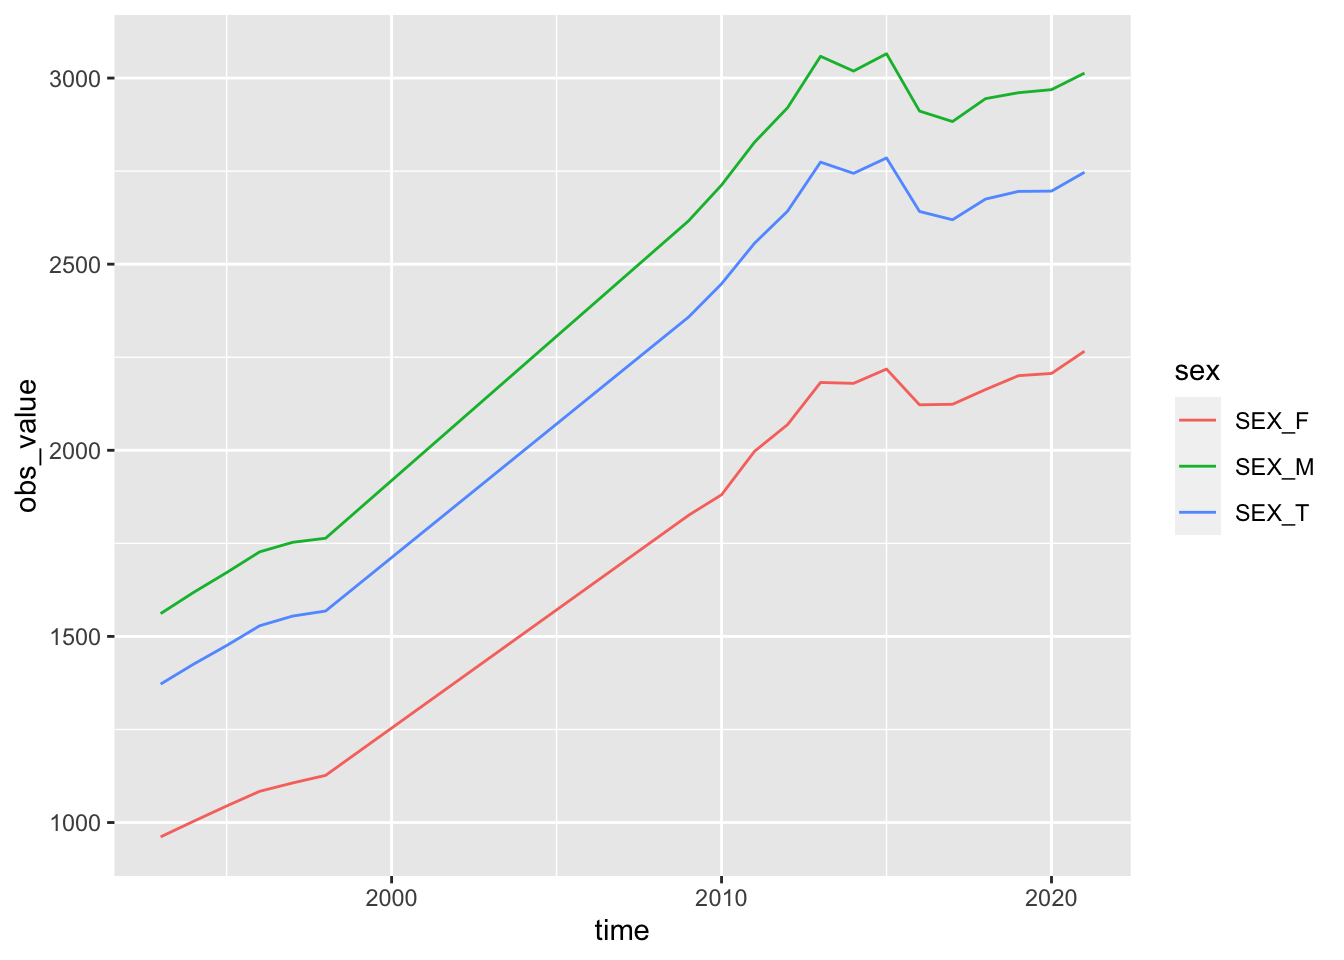
\includegraphics{rstudio_primers_files/figure-latex/unnamed-chunk-13-1.pdf}

\begin{verbatim}
"Good work! What happened to the SUVs? ggplot2 will only use six shapes at a time. By default, additional groups will go unplotted when you use the shape aesthetic. So only use it when you have fewer than seven groups."
\end{verbatim}

\hypertarget{exercise-1-1}{%
\paragraph{Exercise 1}\label{exercise-1-1}}

In the code below, map cty, which is a continuous variable, to color,
size, and shape. How do these aesthetics behave differently for
continuous variables, like cty, vs.~categorical variables, like class?

\begin{verbatim}
# Map cty to color
ggplot(data = mpg) + 
  geom_point(mapping = aes(x = displ, y = hwy))

# Map cty to size
ggplot(data = mpg) + 
  geom_point(mapping = aes(x = displ, y = hwy))

# Map cty to shape
ggplot(data = mpg) + 
  geom_point(mapping = aes(x = displ, y = hwy))
\end{verbatim}

\begin{Shaded}
\begin{Highlighting}[]
\CommentTok{\# Map cty to color}
\FunctionTok{ggplot}\NormalTok{(}\AttributeTok{data =}\NormalTok{ mpg) }\SpecialCharTok{+} 
  \FunctionTok{geom\_point}\NormalTok{(}\AttributeTok{mapping =} \FunctionTok{aes}\NormalTok{(}\AttributeTok{x =}\NormalTok{ displ, }\AttributeTok{y =}\NormalTok{ hwy, }\AttributeTok{color =}\NormalTok{ cty))}
\end{Highlighting}
\end{Shaded}

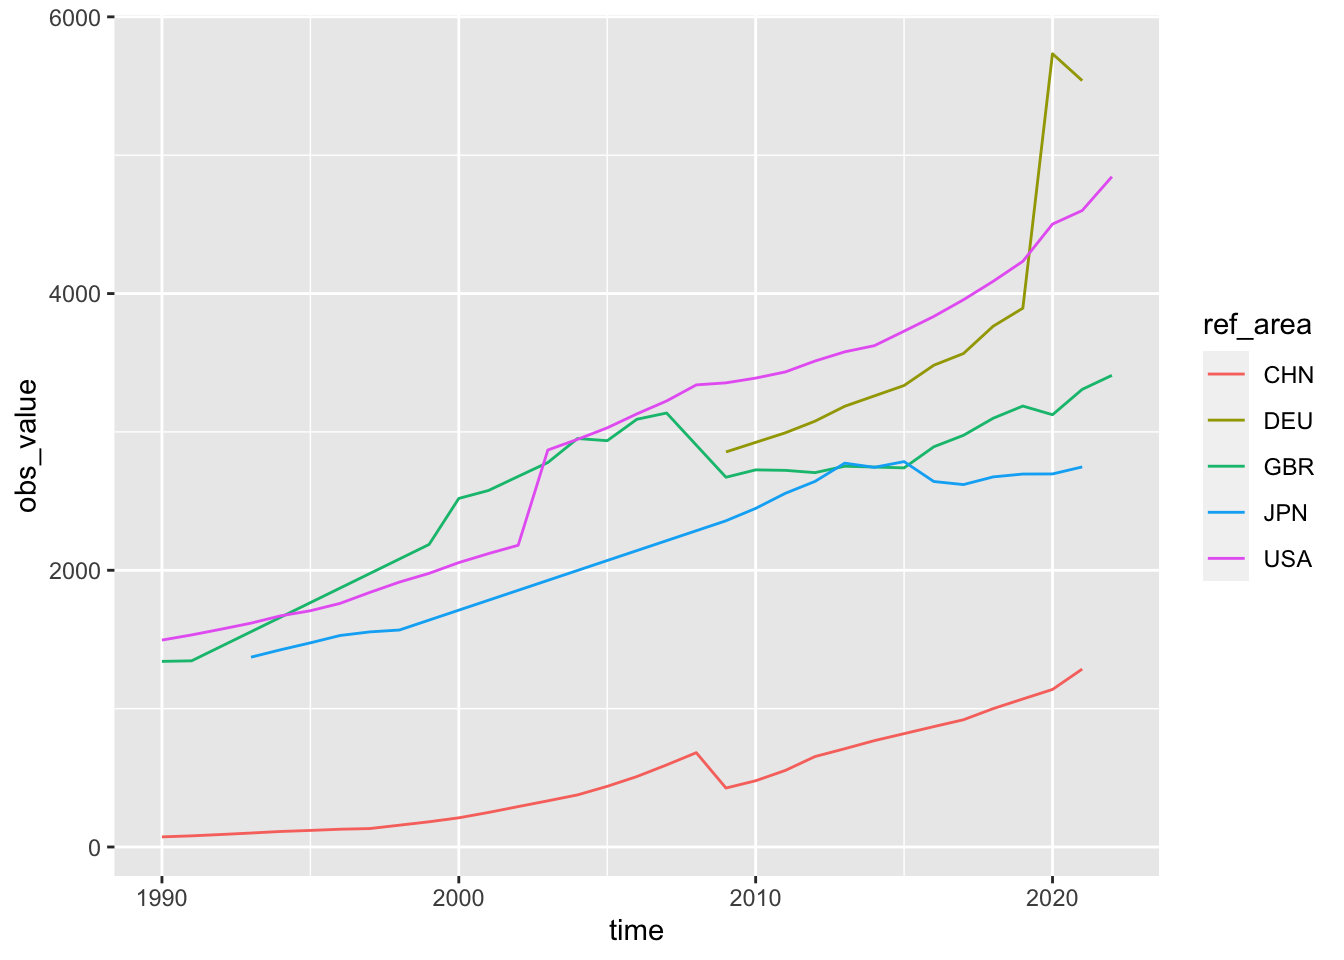
\includegraphics{rstudio_primers_files/figure-latex/unnamed-chunk-14-1.pdf}

\begin{Shaded}
\begin{Highlighting}[]
\CommentTok{\# Map cty to size}
\FunctionTok{ggplot}\NormalTok{(}\AttributeTok{data =}\NormalTok{ mpg) }\SpecialCharTok{+} 
  \FunctionTok{geom\_point}\NormalTok{(}\AttributeTok{mapping =} \FunctionTok{aes}\NormalTok{(}\AttributeTok{x =}\NormalTok{ displ, }\AttributeTok{y =}\NormalTok{ hwy, }\AttributeTok{size =}\NormalTok{ cty))}
\end{Highlighting}
\end{Shaded}

\includegraphics{rstudio_primers_files/figure-latex/unnamed-chunk-14-2.pdf}

\begin{verbatim}
# Map cty to shape
ggplot(data = mpg) + 
  geom_point(mapping = aes(x = displ, y = hwy, shape = cty))
\end{verbatim}

\begin{verbatim}
A continuous variable can not be mapped to shape
\end{verbatim}

\begin{Shaded}
\begin{Highlighting}[]
\FunctionTok{ggplot}\NormalTok{(}\AttributeTok{data =}\NormalTok{ mpg) }\SpecialCharTok{+} 
  \FunctionTok{geom\_point}\NormalTok{(}\AttributeTok{mapping =} \FunctionTok{aes}\NormalTok{(}\AttributeTok{x =}\NormalTok{ displ, }\AttributeTok{y =}\NormalTok{ hwy, }\AttributeTok{shape =}\NormalTok{ class))}
\end{Highlighting}
\end{Shaded}

\begin{verbatim}
## Warning: The shape palette can deal with a maximum of 6 discrete values because
## more than 6 becomes difficult to discriminate; you have 7. Consider
## specifying shapes manually if you must have them.
\end{verbatim}

\begin{verbatim}
## Warning: Removed 62 rows containing missing values (`geom_point()`).
\end{verbatim}

\includegraphics{rstudio_primers_files/figure-latex/unnamed-chunk-15-1.pdf}

\begin{verbatim}
"Very nice! ggplot2 treats continuous and categorical variables differently. Noteably, ggplot2 supplies a blue gradient when you map a continuous variable to color, and ggplot2 will not map continuous variables to shape."
\end{verbatim}

\hypertarget{exercise-2-1}{%
\paragraph{Exercise 2}\label{exercise-2-1}}

Map class to color, size, and shape all in the same plot. Does it work?

\begin{verbatim}
ggplot(data = mpg) + 
  geom_point(mapping = aes(x = displ, y = hwy))
\end{verbatim}

\begin{Shaded}
\begin{Highlighting}[]
\FunctionTok{ggplot}\NormalTok{(}\AttributeTok{data =}\NormalTok{ mpg) }\SpecialCharTok{+} 
  \FunctionTok{geom\_point}\NormalTok{(}\AttributeTok{mapping =} \FunctionTok{aes}\NormalTok{(}\AttributeTok{x =}\NormalTok{ displ, }\AttributeTok{y =}\NormalTok{ hwy, }\AttributeTok{color =}\NormalTok{ class, }\AttributeTok{size =}\NormalTok{ class, }\AttributeTok{shape =}\NormalTok{ class))}
\end{Highlighting}
\end{Shaded}

\begin{verbatim}
## Warning: Using size for a discrete variable is not advised.
\end{verbatim}

\begin{verbatim}
## Warning: The shape palette can deal with a maximum of 6 discrete values because
## more than 6 becomes difficult to discriminate; you have 7. Consider
## specifying shapes manually if you must have them.
\end{verbatim}

\begin{verbatim}
## Warning: Removed 62 rows containing missing values (`geom_point()`).
\end{verbatim}

\includegraphics{rstudio_primers_files/figure-latex/unnamed-chunk-16-1.pdf}

\begin{verbatim}
"Very nice! ggplot2 can map the same variable to multiple aesthetics."
\end{verbatim}

\hypertarget{exercise-3-1}{%
\paragraph{Exercise 3}\label{exercise-3-1}}

What happens if you map an aesthetic to something other than a variable
name, like aes(colour = displ \textless{} 5)? Try it.

\begin{verbatim}
ggplot(data = mpg) + 
  geom_point(mapping = aes(x = displ, y = hwy))
\end{verbatim}

\begin{Shaded}
\begin{Highlighting}[]
\FunctionTok{ggplot}\NormalTok{(}\AttributeTok{data =}\NormalTok{ mpg) }\SpecialCharTok{+} 
  \FunctionTok{geom\_point}\NormalTok{(}\AttributeTok{mapping =} \FunctionTok{aes}\NormalTok{(}\AttributeTok{x =}\NormalTok{ displ, }\AttributeTok{y =}\NormalTok{ hwy, }\AttributeTok{color =}\NormalTok{ displ }\SpecialCharTok{\textless{}} \DecValTok{5}\NormalTok{))}
\end{Highlighting}
\end{Shaded}

\includegraphics{rstudio_primers_files/figure-latex/unnamed-chunk-17-1.pdf}

\begin{verbatim}
"Good job! ggplot2 will map the aesthetic to the results of the expression. Here, ggplot2 mapped the color of each point to TRUE or FALSE based on whther the point's `displ` value was less than five."
\end{verbatim}

\hypertarget{setting-aesthetics}{%
\paragraph{Setting aesthetics}\label{setting-aesthetics}}

What if you just want to make all of the points in your plot blue, like
in the plot below?

\includegraphics{./data/unnamed-chunk-8-1.png} You can do this by
setting the color aesthetic outside of the aes() function, like this

\begin{Shaded}
\begin{Highlighting}[]
\FunctionTok{ggplot}\NormalTok{(}\AttributeTok{data =}\NormalTok{ mpg) }\SpecialCharTok{+}
  \FunctionTok{geom\_point}\NormalTok{(}\AttributeTok{mapping =} \FunctionTok{aes}\NormalTok{(}\AttributeTok{x =}\NormalTok{ displ, }\AttributeTok{y =}\NormalTok{ hwy), }\AttributeTok{color =} \StringTok{"blue"}\NormalTok{)}
\end{Highlighting}
\end{Shaded}

\includegraphics{rstudio_primers_files/figure-latex/unnamed-chunk-18-1.pdf}

\hypertarget{setting-vs.-mapping}{%
\paragraph{Setting vs.~Mapping}\label{setting-vs.-mapping}}

Setting works for every aesthetic in ggplot2. If you want to manually
set the aesthetic to a value in the visual space, set the aesthetic
outside of aes().

\begin{Shaded}
\begin{Highlighting}[]
\FunctionTok{ggplot}\NormalTok{(}\AttributeTok{data =}\NormalTok{ mpg) }\SpecialCharTok{+}
  \FunctionTok{geom\_point}\NormalTok{(}\AttributeTok{mapping =} \FunctionTok{aes}\NormalTok{(}\AttributeTok{x =}\NormalTok{ displ, }\AttributeTok{y =}\NormalTok{ hwy), }\AttributeTok{color =} \StringTok{"blue"}\NormalTok{, }\AttributeTok{shape =} \DecValTok{3}\NormalTok{, }\AttributeTok{alpha =} \FloatTok{0.5}\NormalTok{)}
\end{Highlighting}
\end{Shaded}

\includegraphics{rstudio_primers_files/figure-latex/unnamed-chunk-19-1.pdf}

If you want to map the aesthetic to a variable in the data space, map
the aesthetic inside aes().

\begin{Shaded}
\begin{Highlighting}[]
\FunctionTok{ggplot}\NormalTok{(}\AttributeTok{data =}\NormalTok{ mpg) }\SpecialCharTok{+}
  \FunctionTok{geom\_point}\NormalTok{(}\AttributeTok{mapping =} \FunctionTok{aes}\NormalTok{(}\AttributeTok{x =}\NormalTok{ displ, }\AttributeTok{y =}\NormalTok{ hwy, }\AttributeTok{color =}\NormalTok{ class, }\AttributeTok{shape =}\NormalTok{ fl, }\AttributeTok{alpha =}\NormalTok{ displ))}
\end{Highlighting}
\end{Shaded}

\includegraphics{rstudio_primers_files/figure-latex/unnamed-chunk-20-1.pdf}

\hypertarget{exercise-4}{%
\paragraph{Exercise 4}\label{exercise-4}}

What do you think went wrong in the code below? Fix the code so it does
something sensible.

\begin{verbatim}
ggplot(data = mpg) +
  geom_point(mapping = aes(x = displ, y = hwy, color = "blue"))
\end{verbatim}

\begin{Shaded}
\begin{Highlighting}[]
\FunctionTok{ggplot}\NormalTok{(}\AttributeTok{data =}\NormalTok{ mpg) }\SpecialCharTok{+}
  \FunctionTok{geom\_point}\NormalTok{(}\AttributeTok{mapping =} \FunctionTok{aes}\NormalTok{(}\AttributeTok{x =}\NormalTok{ displ, }\AttributeTok{y =}\NormalTok{ hwy), }\AttributeTok{color =} \StringTok{"blue"}\NormalTok{)}
\end{Highlighting}
\end{Shaded}

\includegraphics{rstudio_primers_files/figure-latex/unnamed-chunk-21-1.pdf}

\begin{verbatim}
"Good job! Putting an aesthetic in the wrong location is one of the most common graphing errors. Sometimes it helps to think of legends. If you will need a legend to understand what the color/shape/etc. means, then you should probably put the aesthetic inside `aes()` --- ggplot2 will build a legend for every aesthetic mapped here. If the aesthetic has no meaning and is just... well, aesthetic, then set it outside of `aes()`."
\end{verbatim}

\hypertarget{recap}{%
\paragraph{Recap}\label{recap}}

For each aesthetic, you associate the name of the aesthetic with a
variable to display, and you do this within aes().

Once you map a variable to an aesthetic, ggplot2 takes care of the rest.
It selects a reasonable scale to use with the aesthetic, and it
constructs a legend that explains the mapping between levels and values.
For x and y aesthetics, ggplot2 does not create a legend, but it creates
an axis line with tick marks and a label. The axis line acts as a
legend; it explains the mapping between locations and values.

You've experimented with the most common aesthetics for points: x, y,
color, size, alpha and shape. Each geom uses its own set of aesthetics
(you wouldn't expect a line to have a shape, for example). To find out
which aesthetics a geom uses, open its help page, e.g.~?geom\_line.

This raises a new question that we've only brushed over: what is a geom?

\hypertarget{geometric-objects}{%
\subsubsection{Geometric objects}\label{geometric-objects}}

\hypertarget{geoms}{%
\paragraph{Geoms}\label{geoms}}

How are these two plots similar?

\includegraphics{./data/unnamed-chunk-9-1.png}
\includegraphics{./data/unnamed-chunk-9-2.png}

Both plots contain the same x variable, the same y variable, and both
describe the same data. But the plots are not identical. Each plot uses
a different visual object to represent the data. In ggplot2 syntax, we
say that they use different geoms.

A geom is the geometrical object that a plot uses to represent
observations. People often describe plots by the type of geom that the
plot uses. For example, bar charts use bar geoms, line charts use line
geoms, boxplots use boxplot geoms, and so on. Scatterplots break the
trend; they use the point geom.

As we see above, you can use different geoms to plot the same data. The
plot on the left uses the point geom, and the plot on the right uses the
smooth geom, a smooth line fitted to the data.

\hypertarget{geom-functions}{%
\paragraph{Geom functions}\label{geom-functions}}

To change the geom in your plot, change the geom function that you add
to ggplot(). For example, take this code which makes the plot on the
left (above), and change geom\_point() to geom\_smooth(). What do you
get?

\begin{verbatim}
ggplot(data = mpg) + 
  geom_point(mapping = aes(x = displ, y = hwy))
\end{verbatim}

\begin{Shaded}
\begin{Highlighting}[]
\FunctionTok{ggplot}\NormalTok{(}\AttributeTok{data =}\NormalTok{ mpg) }\SpecialCharTok{+} 
  \FunctionTok{geom\_smooth}\NormalTok{(}\AttributeTok{mapping =} \FunctionTok{aes}\NormalTok{(}\AttributeTok{x =}\NormalTok{ displ, }\AttributeTok{y =}\NormalTok{ hwy))}
\end{Highlighting}
\end{Shaded}

\begin{verbatim}
## `geom_smooth()` using method = 'loess' and formula = 'y ~ x'
\end{verbatim}

\includegraphics{rstudio_primers_files/figure-latex/unnamed-chunk-22-1.pdf}

\begin{verbatim}
"Good job! You get the plot on the right (above)."
\end{verbatim}

\hypertarget{more-about-geoms}{%
\paragraph{More about geoms}\label{more-about-geoms}}

ggplot2 provides over 30 geom functions that you can use to make plots,
and extension packages provide even more (see
\url{https://exts.ggplot2.tidyverse.org/gallery/} for a sampling).
You'll learn how to use these geoms to explore data in the Visualize
Data primer.

Until then, the best way to get a comprehensive overview of the
available geoms is with the
\href{https://www.rstudio.com/wp-content/uploads/2016/11/ggplot2-cheatsheet-2.1.pdf}{ggplot2
cheatsheet}. To learn more about any single geom, look at its help page,
e.g.~?geom\_smooth.

\hypertarget{exercise-1-2}{%
\paragraph{Exercise 1}\label{exercise-1-2}}

What geom would you use to draw a line chart? A boxplot? A histogram? An
area chart?

\hypertarget{exercise-2-2}{%
\paragraph{Exercise 2}\label{exercise-2-2}}

\textbf{What does the se argument to geom\_smooth() do?}

\begin{itemize}
\tightlist
\item
  Nothing. se is not an argument of geom\_smooth() ✗
\item
  chooses a method for calculating the smooth line ✗
\item
  controls whether or not to show errors ✗
\item[$\boxtimes$]
  Adds or removes a standard error ribbon around the smooth line ✓
\end{itemize}

\hypertarget{putting-it-all-together}{%
\paragraph{Putting it all together}\label{putting-it-all-together}}

The ideas that you've learned here: geoms, aesthetics, and the implied
existence of a data space and a visual space combine to form a system
known as the Grammar of Graphics.

The Grammar of Graphics provides a systematic way to build any graph,
and it underlies the ggplot2 package. In fact, the first two letters of
ggplot2 stand for ``Grammar of Graphics''.

\hypertarget{the-grammar-of-graphics}{%
\paragraph{The Grammar of Graphics}\label{the-grammar-of-graphics}}

The best way to understand the Grammar of Graphics is to see it
explained in action:

Video: \url{https://vimeo.com/223812632}

\hypertarget{the-ggplot2-package}{%
\subsubsection{The ggplot2 package}\label{the-ggplot2-package}}

What is a package?

Throughout this tutorial, I've referred to ggplot2 as a package. What
does that mean?

The R language is subdivided into packages, small collections of data
sets and functions that all focus on a single task. The functions that
we used in this tutorial come from one of those packages, the ggplot2
package, which focuses on visualizing data.

\hypertarget{what-should-you-know-about-packages}{%
\paragraph{What should you know about
packages?}\label{what-should-you-know-about-packages}}

When you first install R, you get a small collection of core packages
known as base R. The remaining packages---there are over 10,000 of
them---are optional. You don't need to install them unless you want to
use them.

ggplot2 is one of these optionals packages, so are the other packages
that we will look at in these tutorials. Some of the most popular and
most modern parts of R come in the optional packages.

You don't need to worry about installing packages in these tutorials.
Each tutorial comes with all of the packages that you need
pre-installed; this is how we make the tutorials easy to use.

However, one day, you may want to use R outside of these tutorials. When
that day comes, you'll want to remember which packages to download to
acquire the functions you use here. Throughout the tutorials, I will try
to make it as clear as possible where each function comes from!

If you'd like to learn more about installing R packages (or R or the
RStudio IDE), the Set Up video tutorial walks you through the process of
setting up R on your own computer.

\hypertarget{where-to-from-here}{%
\paragraph{Where to from here}\label{where-to-from-here}}

Congratulations! You can use the ggplot2 code template to plot any
dataset in many different ways. As you begin exploring data, you should
incorporate these tools into your workflow.

There is much more to ggplot2 and Data Visualization than we have
covered here. If you would like to learn more about visualizing data
with ggplot2, check out RStudio's primer on Data Visualization.

Your new data visualization skills will make it easier to learn other
parts of R, because you can now visualize the results of any change that
you make to data. you'll put these skills to immediate use in the next
tutorial, which will show you how to extract values from datasets, as
well as how to compute new variables and summary statistics from your
data. See you there.

\hypertarget{programming-basics}{%
\subsection{Programming Basics}\label{programming-basics}}

This tutorial demystifies programming with R. Here, you'll learn how to
run functions and build objects.

\hypertarget{welcome-1}{%
\subsubsection{Welcome}\label{welcome-1}}

\hypertarget{welcome-to-r}{%
\paragraph{Welcome to R}\label{welcome-to-r}}

R is easiest to use when you know how the R language works. This
tutorial will teach you the implicit background knowledge that informs
every piece of R code. You'll learn about:

\begin{itemize}
\tightlist
\item
  functions and their arguments objects
\item
  R's basic data types
\item
  R's basic data structures including vectors and lists
\item
  R's package system
\end{itemize}

\hypertarget{functions}{%
\subsubsection{Functions}\label{functions}}

\hypertarget{functions-1}{%
\paragraph{Functions}\label{functions-1}}

Video: \url{https://vimeo.com/220490105}

\hypertarget{run-a-function}{%
\paragraph{Run a function}\label{run-a-function}}

Can you use the sqrt() function in the chunk below to compute the square
root of 962?

\begin{Shaded}
\begin{Highlighting}[]
\FunctionTok{sqrt}\NormalTok{(}\DecValTok{962}\NormalTok{)}
\end{Highlighting}
\end{Shaded}

\begin{verbatim}
## [1] 31.01612
\end{verbatim}

\hypertarget{code}{%
\paragraph{Code}\label{code}}

Use the code chunk below to examine the code that sqrt() runs.

\begin{Shaded}
\begin{Highlighting}[]
\NormalTok{sqrt}
\end{Highlighting}
\end{Shaded}

\begin{verbatim}
## function (x)  .Primitive("sqrt")
\end{verbatim}

\begin{verbatim}
"Good job! sqrt immediately triggers a low level algorithm optimized for performance, so there is not much code to see."
\end{verbatim}

\hypertarget{lm}{%
\paragraph{lm}\label{lm}}

Compare the code in sqrt() to the code in another R function, lm().
Examine lm()'s code body in the chunk below.

\begin{Shaded}
\begin{Highlighting}[]
\NormalTok{lm}
\end{Highlighting}
\end{Shaded}

\begin{verbatim}
## function (formula, data, subset, weights, na.action, method = "qr", 
##     model = TRUE, x = FALSE, y = FALSE, qr = TRUE, singular.ok = TRUE, 
##     contrasts = NULL, offset, ...) 
## {
##     ret.x <- x
##     ret.y <- y
##     cl <- match.call()
##     mf <- match.call(expand.dots = FALSE)
##     m <- match(c("formula", "data", "subset", "weights", "na.action", 
##         "offset"), names(mf), 0L)
##     mf <- mf[c(1L, m)]
##     mf$drop.unused.levels <- TRUE
##     mf[[1L]] <- quote(stats::model.frame)
##     mf <- eval(mf, parent.frame())
##     if (method == "model.frame") 
##         return(mf)
##     else if (method != "qr") 
##         warning(gettextf("method = '%s' is not supported. Using 'qr'", 
##             method), domain = NA)
##     mt <- attr(mf, "terms")
##     y <- model.response(mf, "numeric")
##     w <- as.vector(model.weights(mf))
##     if (!is.null(w) && !is.numeric(w)) 
##         stop("'weights' must be a numeric vector")
##     offset <- model.offset(mf)
##     mlm <- is.matrix(y)
##     ny <- if (mlm) 
##         nrow(y)
##     else length(y)
##     if (!is.null(offset)) {
##         if (!mlm) 
##             offset <- as.vector(offset)
##         if (NROW(offset) != ny) 
##             stop(gettextf("number of offsets is %d, should equal %d (number of observations)", 
##                 NROW(offset), ny), domain = NA)
##     }
##     if (is.empty.model(mt)) {
##         x <- NULL
##         z <- list(coefficients = if (mlm) matrix(NA_real_, 0, 
##             ncol(y)) else numeric(), residuals = y, fitted.values = 0 * 
##             y, weights = w, rank = 0L, df.residual = if (!is.null(w)) sum(w != 
##             0) else ny)
##         if (!is.null(offset)) {
##             z$fitted.values <- offset
##             z$residuals <- y - offset
##         }
##     }
##     else {
##         x <- model.matrix(mt, mf, contrasts)
##         z <- if (is.null(w)) 
##             lm.fit(x, y, offset = offset, singular.ok = singular.ok, 
##                 ...)
##         else lm.wfit(x, y, w, offset = offset, singular.ok = singular.ok, 
##             ...)
##     }
##     class(z) <- c(if (mlm) "mlm", "lm")
##     z$na.action <- attr(mf, "na.action")
##     z$offset <- offset
##     z$contrasts <- attr(x, "contrasts")
##     z$xlevels <- .getXlevels(mt, mf)
##     z$call <- cl
##     z$terms <- mt
##     if (model) 
##         z$model <- mf
##     if (ret.x) 
##         z$x <- x
##     if (ret.y) 
##         z$y <- y
##     if (!qr) 
##         z$qr <- NULL
##     z
## }
## <bytecode: 0x13918c828>
## <environment: namespace:stats>
\end{verbatim}

\hypertarget{help-pages}{%
\paragraph{help pages}\label{help-pages}}

Wow! lm() runs a lot of code. What does it do? Open the help page for
lm() in the chunk below and find out.

\begin{verbatim}
? lm
\end{verbatim}

\begin{verbatim}
lm {stats}  R Documentation
Fitting Linear Models
Description
lm is used to fit linear models. It can be used to carry out regression, single stratum analysis of variance and analysis of covariance (although aov may provide a more convenient interface for these).

Usage
lm(formula, data, subset, weights, na.action,
   method = "qr", model = TRUE, x = FALSE, y = FALSE, qr = TRUE,
   singular.ok = TRUE, contrasts = NULL, offset, ...)
Arguments
formula 
an object of class "formula" (or one that can be coerced to that class): a symbolic description of the model to be fitted. The details of model specification are given under ‘Details’.

data    
an optional data frame, list or environment (or object coercible by as.data.frame to a data frame) containing the variables in the model. If not found in data, the variables are taken from environment(formula), typically the environment from which lm is called.

subset  
an optional vector specifying a subset of observations to be used in the fitting process.

weights 
an optional vector of weights to be used in the fitting process. Should be NULL or a numeric vector. If non-NULL, weighted least squares is used with weights weights (that is, minimizing sum(w*e^2)); otherwise ordinary least squares is used. See also ‘Details’,

na.action   
a function which indicates what should happen when the data contain NAs. The default is set by the na.action setting of options, and is na.fail if that is unset. The ‘factory-fresh’ default is na.omit. Another possible value is NULL, no action. Value na.exclude can be useful.

method  
the method to be used; for fitting, currently only method = "qr" is supported; method = "model.frame" returns the model frame (the same as with model = TRUE, see below).

model, x, y, qr 
logicals. If TRUE the corresponding components of the fit (the model frame, the model matrix, the response, the QR decomposition) are returned.

singular.ok 
logical. If FALSE (the default in S but not in R) a singular fit is an error.

contrasts   
an optional list. See the contrasts.arg of model.matrix.default.

offset  
this can be used to specify an a priori known component to be included in the linear predictor during fitting. This should be NULL or a numeric vector or matrix of extents matching those of the response. One or more offset terms can be included in the formula instead or as well, and if more than one are specified their sum is used. See model.offset.

... 
additional arguments to be passed to the low level regression fitting functions (see below).

Details
Models for lm are specified symbolically. A typical model has the form response ~ terms where response is the (numeric) response vector and terms is a series of terms which specifies a linear predictor for response. A terms specification of the form first + second indicates all the terms in first together with all the terms in second with duplicates removed. A specification of the form first:second indicates the set of terms obtained by taking the interactions of all terms in first with all terms in second. The specification first*second indicates the cross of first and second. This is the same as first + second + first:second.

If the formula includes an offset, this is evaluated and subtracted from the response.

If response is a matrix a linear model is fitted separately by least-squares to each column of the matrix.

See model.matrix for some further details. The terms in the formula will be re-ordered so that main effects come first, followed by the interactions, all second-order, all third-order and so on: to avoid this pass a terms object as the formula (see aov and demo(glm.vr) for an example).

A formula has an implied intercept term. To remove this use either y ~ x - 1 or y ~ 0 + x. See formula for more details of allowed formulae.

Non-NULL weights can be used to indicate that different observations have different variances (with the values in weights being inversely proportional to the variances); or equivalently, when the elements of weights are positive integers w_i, that each response y_i is the mean of w_i unit-weight observations (including the case that there are w_i observations equal to y_i and the data have been summarized). However, in the latter case, notice that within-group variation is not used. Therefore, the sigma estimate and residual degrees of freedom may be suboptimal; in the case of replication weights, even wrong. Hence, standard errors and analysis of variance tables should be treated with care.

lm calls the lower level functions lm.fit, etc, see below, for the actual numerical computations. For programming only, you may consider doing likewise.

All of weights, subset and offset are evaluated in the same way as variables in formula, that is first in data and then in the environment of formula.

Value
lm returns an object of class "lm" or for multiple responses of class c("mlm", "lm").

The functions summary and anova are used to obtain and print a summary and analysis of variance table of the results. The generic accessor functions coefficients, effects, fitted.values and residuals extract various useful features of the value returned by lm.

An object of class "lm" is a list containing at least the following components:

coefficients    
a named vector of coefficients

residuals   
the residuals, that is response minus fitted values.

fitted.values   
the fitted mean values.

rank    
the numeric rank of the fitted linear model.

weights 
(only for weighted fits) the specified weights.

df.residual 
the residual degrees of freedom.

call    
the matched call.

terms   
the terms object used.

contrasts   
(only where relevant) the contrasts used.

xlevels 
(only where relevant) a record of the levels of the factors used in fitting.

offset  
the offset used (missing if none were used).

y   
if requested, the response used.

x   
if requested, the model matrix used.

model   
if requested (the default), the model frame used.

na.action   
(where relevant) information returned by model.frame on the special handling of NAs.

In addition, non-null fits will have components assign, effects and (unless not requested) qr relating to the linear fit, for use by extractor functions such as summary and effects.

Using time series
Considerable care is needed when using lm with time series.

Unless na.action = NULL, the time series attributes are stripped from the variables before the regression is done. (This is necessary as omitting NAs would invalidate the time series attributes, and if NAs are omitted in the middle of the series the result would no longer be a regular time series.)

Even if the time series attributes are retained, they are not used to line up series, so that the time shift of a lagged or differenced regressor would be ignored. It is good practice to prepare a data argument by ts.intersect(..., dframe = TRUE), then apply a suitable na.action to that data frame and call lm with na.action = NULL so that residuals and fitted values are time series.

Note
Offsets specified by offset will not be included in predictions by predict.lm, whereas those specified by an offset term in the formula will be.

Author(s)
The design was inspired by the S function of the same name described in Chambers (1992). The implementation of model formula by Ross Ihaka was based on Wilkinson & Rogers (1973).

References
Chambers, J. M. (1992) Linear models. Chapter 4 of Statistical Models in S eds J. M. Chambers and T. J. Hastie, Wadsworth & Brooks/Cole.

Wilkinson, G. N. and Rogers, C. E. (1973). Symbolic descriptions of factorial models for analysis of variance. Applied Statistics, 22, 392–399. doi: 10.2307/2346786.

See Also
summary.lm for summaries and anova.lm for the ANOVA table; aov for a different interface.

The generic functions coef, effects, residuals, fitted, vcov.

predict.lm (via predict) for prediction, including confidence and prediction intervals; confint for confidence intervals of parameters.

lm.influence for regression diagnostics, and glm for generalized linear models.

The underlying low level functions, lm.fit for plain, and lm.wfit for weighted regression fitting.

More lm() examples are available e.g., in anscombe, attitude, freeny, LifeCycleSavings, longley, stackloss, swiss.

biglm in package biglm for an alternative way to fit linear models to large datasets (especially those with many cases).

Examples
require(graphics)

## Annette Dobson (1990) "An Introduction to Generalized Linear Models".
## Page 9: Plant Weight Data.
ctl <- c(4.17,5.58,5.18,6.11,4.50,4.61,5.17,4.53,5.33,5.14)
trt <- c(4.81,4.17,4.41,3.59,5.87,3.83,6.03,4.89,4.32,4.69)
group <- gl(2, 10, 20, labels = c("Ctl","Trt"))
weight <- c(ctl, trt)
lm.D9 <- lm(weight ~ group)
lm.D90 <- lm(weight ~ group - 1) # omitting intercept

anova(lm.D9)
summary(lm.D90)

opar <- par(mfrow = c(2,2), oma = c(0, 0, 1.1, 0))
plot(lm.D9, las = 1)      # Residuals, Fitted, ...
par(opar)

### less simple examples in "See Also" above
[Package stats version 4.0.3 Index]
\end{verbatim}

\begin{verbatim}
"Good job! `lm()` is R's function for fitting basic linear models. No wonder it runs so much code.
\end{verbatim}

\hypertarget{code-comments}{%
\paragraph{Code comments}\label{code-comments}}

What do you think the chunk below will return? Run it and see. The
result should be nothing. R will not run anything on a line after a \#
symbol. This is useful because it lets you write human readable comments
in your code: just place the comments after a \#. Now delete the \# and
re-run the chunk. You should see a result.

\begin{Shaded}
\begin{Highlighting}[]
\CommentTok{\# sqrt(961)}
\end{Highlighting}
\end{Shaded}

\begin{Shaded}
\begin{Highlighting}[]
\FunctionTok{sqrt}\NormalTok{(}\DecValTok{961}\NormalTok{)}
\end{Highlighting}
\end{Shaded}

\begin{verbatim}
## [1] 31
\end{verbatim}

\hypertarget{arguments}{%
\subsubsection{Arguments}\label{arguments}}

\hypertarget{arguments-1}{%
\paragraph{Arguments}\label{arguments-1}}

Video: \url{https://vimeo.com/220490157}

\hypertarget{args}{%
\paragraph{args()}\label{args}}

rnorm() is a function that generates random variables from a normal
distribution. Find the arguments of rnorm()

\begin{Shaded}
\begin{Highlighting}[]
\FunctionTok{args}\NormalTok{(rnorm)}
\end{Highlighting}
\end{Shaded}

\begin{verbatim}
## function (n, mean = 0, sd = 1) 
## NULL
\end{verbatim}

\begin{verbatim}
"Good job! `n` specifies the number of random normal variables to generate. `mean` and `sd` describe the distribution to generate the random values with."
\end{verbatim}

\hypertarget{optional-arguments}{%
\paragraph{optional arguments}\label{optional-arguments}}

\textbf{Which arguments of R norm are optional?}

\begin{itemize}
\tightlist
\item[$\square$]
  n ✗
\item[$\boxtimes$]
  mean ✓
\item[$\boxtimes$]
  sd ✓
\end{itemize}

n is not an optional argument because it does not have a default value.

\hypertarget{rnorm-1}{%
\paragraph{rnorm() 1}\label{rnorm-1}}

Use rnrom() to generate 100 random normal values with a mean of 100 and
a standard deviation of 15.

\begin{Shaded}
\begin{Highlighting}[]
\FunctionTok{rnorm}\NormalTok{(}\DecValTok{100}\NormalTok{, }\AttributeTok{mean =} \DecValTok{100}\NormalTok{, }\AttributeTok{sd =} \DecValTok{15}\NormalTok{)}
\end{Highlighting}
\end{Shaded}

\begin{verbatim}
##   [1]  63.95632 116.27276 106.08390  99.80621  79.66732 111.97160  89.67638
##   [8] 101.79404  70.62430  87.96299 143.04064  93.05035 115.62439  88.85849
##  [15] 119.78149  89.02004 102.97381  94.04783 100.14924  79.33365  94.89680
##  [22]  73.94401 119.20848  80.94186 104.78484  82.73381  89.55936 103.34303
##  [29] 104.28356  92.55336  95.87462  85.36085  83.64231 119.28289 114.19642
##  [36] 101.24286 124.33488  99.20985  96.76189 104.14935  80.40709 113.68612
##  [43]  79.40248  89.92031  97.25959 106.04484 106.17672 104.33271 105.04684
##  [50] 129.65419 107.75165  99.32673 105.09378 110.10952  93.41995 113.43911
##  [57]  99.60066  85.23298 111.22401 113.15320  87.80174 105.16080  84.79331
##  [64]  80.35354  97.83126 117.00526 105.42322 102.45910  97.25287  88.47663
##  [71]  99.77702  72.52276 118.47690 123.11281  55.99309 131.88691  95.71034
##  [78] 102.15181 124.35868  81.27119  95.06583 102.31053 108.63178  94.88095
##  [85] 121.21468 106.53382 126.25321 115.89817  72.34626  95.50081 107.36546
##  [92] 102.30802  95.78458 104.66147  97.52274 117.88014  98.38045 102.29912
##  [99]  81.20176 128.88931
\end{verbatim}

\hypertarget{rnorm-2}{%
\paragraph{rnorm() 2}\label{rnorm-2}}

Can you spot the error in the code below? Fix the code and then re-run
it.

\begin{verbatim}
rnorm(100, mu = 100, sd = 50)
\end{verbatim}

\begin{Shaded}
\begin{Highlighting}[]
\FunctionTok{rnorm}\NormalTok{(}\DecValTok{100}\NormalTok{, }\AttributeTok{mean =} \DecValTok{100}\NormalTok{, }\AttributeTok{sd =} \DecValTok{50}\NormalTok{)}
\end{Highlighting}
\end{Shaded}

\begin{verbatim}
##   [1] 124.72160 183.41181 104.17936  97.71649 101.00379 122.60001 103.25660
##   [8]  16.91681  42.00049  89.74771 142.29401 137.34866  12.60537 133.43971
##  [15] 142.24151  56.46558 -18.19024  66.35181  98.91481  66.90316  75.72583
##  [22]  48.69730  67.25951  69.06202 148.25661  97.91540  58.88236 145.84322
##  [29]  85.27540  61.48074  81.50989  36.29291  92.22339 132.96650 134.18211
##  [36] 144.02353  97.66919 166.57355  94.23869  21.69034 126.78450  67.93270
##  [43] 113.06072  60.54486  79.13573 129.01498 103.99898  75.94946  98.57054
##  [50] 133.60217 -35.77817 165.91952 100.37000 104.97527  69.00670  15.65247
##  [57]  74.06364 107.62778 142.24155  74.43713 135.30593  65.01128  77.53792
##  [64]  54.30067 -41.92387 153.13922 115.59614 120.88498 217.22286 120.84782
##  [71] 128.01383  54.38254 106.04201  17.78663 145.31607 107.95615  93.69182
##  [78]  67.46741  38.36551  60.00720  81.37042  81.60824 106.99989 141.16099
##  [85] 205.81188  37.82849  34.56466 131.71531  68.64661  55.07483  84.39364
##  [92] 138.61056 142.19825  20.60434 142.76473 127.52130  10.59611  99.21276
##  [99] 141.42130 146.20675
\end{verbatim}

\hypertarget{objects}{%
\subsubsection{Objects}\label{objects}}

\hypertarget{objects-1}{%
\paragraph{Objects}\label{objects-1}}

Video: \url{https://vimeo.com/220493412}

\hypertarget{object-names}{%
\paragraph{Object names}\label{object-names}}

You can choose almost any name you like for an object, as long as the
name does not begin with a number or a special character like +, -, *,
/, \^{}, !, @, or \&.

\textbf{Which of these would be valid object names?}

\begin{itemize}
\tightlist
\item[$\boxtimes$]
  today ✓
\item[$\square$]
  1st ✗
\item[$\square$]
  +1 ✗
\item[$\boxtimes$]
  vars ✓
\item[$\square$]
  \^{}\_\^{} ✗
\item[$\boxtimes$]
  foo ✓
\end{itemize}

\begin{verbatim}
Remember that the most helpful names will remind you what you put in your object.
\end{verbatim}

\hypertarget{using-objects}{%
\paragraph{Using objects}\label{using-objects}}

In the code chunk below, save the results of rnorm(100, mean = 100, sd =
15) to an object named data. Then, on a new line, call the hist()
function on data to plot a histogram of the random values.

\begin{Shaded}
\begin{Highlighting}[]
\NormalTok{data }\OtherTok{\textless{}{-}} \FunctionTok{rnorm}\NormalTok{(}\DecValTok{100}\NormalTok{, }\AttributeTok{mean =} \DecValTok{100}\NormalTok{, }\AttributeTok{sd =} \DecValTok{15}\NormalTok{)}
\FunctionTok{hist}\NormalTok{(data)}
\end{Highlighting}
\end{Shaded}

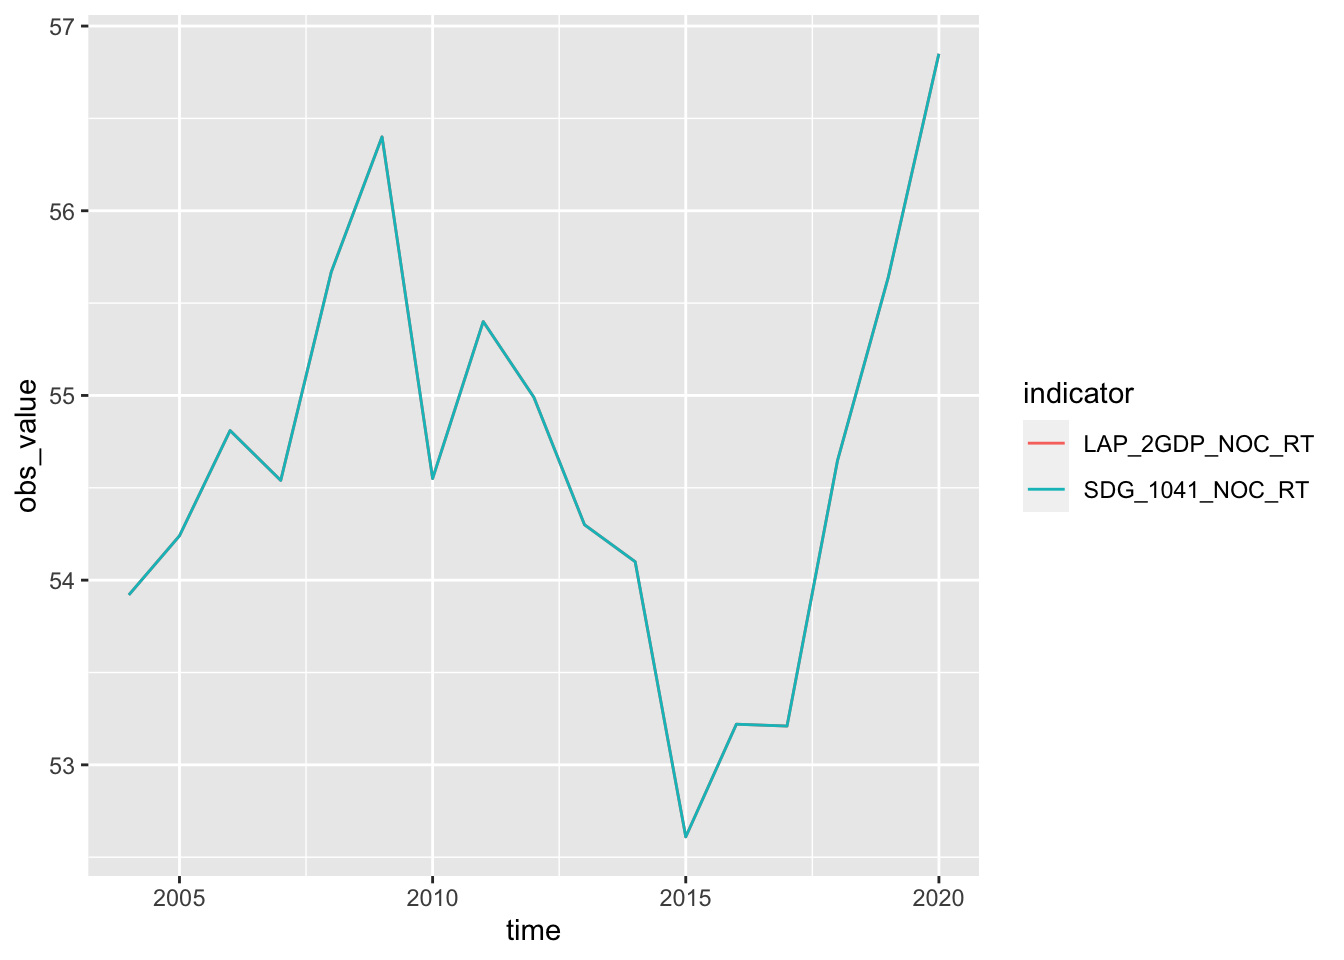
\includegraphics{rstudio_primers_files/figure-latex/unnamed-chunk-31-1.pdf}

\hypertarget{what-if}{%
\paragraph{What if?}\label{what-if}}

What do you think would happen if you assigned data to a new object
named copy, like this? Run the code and then inspect both data and copy.

\begin{Shaded}
\begin{Highlighting}[]
\NormalTok{data }\OtherTok{\textless{}{-}} \FunctionTok{rnorm}\NormalTok{(}\DecValTok{100}\NormalTok{, }\AttributeTok{mean =} \DecValTok{100}\NormalTok{, }\AttributeTok{sd =} \DecValTok{15}\NormalTok{)}
\NormalTok{copy }\OtherTok{\textless{}{-}}\NormalTok{ data}
\FunctionTok{identical}\NormalTok{(copy, data)}
\end{Highlighting}
\end{Shaded}

\begin{verbatim}
## [1] TRUE
\end{verbatim}

\begin{verbatim}
"Good job! R saves a copy of the contents in data to copy."
\end{verbatim}

\hypertarget{data-sets}{%
\paragraph{Data sets}\label{data-sets}}

Objects provide an easy way to store data sets in R. In fact, R comes
with many toy data sets pre-loaded. Examine the contents of iris to see
a classic toy data set. Hint: how could you learn more about the iris
object?

\begin{Shaded}
\begin{Highlighting}[]
\NormalTok{iris}
\end{Highlighting}
\end{Shaded}

\begin{verbatim}
##     Sepal.Length Sepal.Width Petal.Length Petal.Width    Species
## 1            5.1         3.5          1.4         0.2     setosa
## 2            4.9         3.0          1.4         0.2     setosa
## 3            4.7         3.2          1.3         0.2     setosa
## 4            4.6         3.1          1.5         0.2     setosa
## 5            5.0         3.6          1.4         0.2     setosa
## 6            5.4         3.9          1.7         0.4     setosa
## 7            4.6         3.4          1.4         0.3     setosa
## 8            5.0         3.4          1.5         0.2     setosa
## 9            4.4         2.9          1.4         0.2     setosa
## 10           4.9         3.1          1.5         0.1     setosa
## 11           5.4         3.7          1.5         0.2     setosa
## 12           4.8         3.4          1.6         0.2     setosa
## 13           4.8         3.0          1.4         0.1     setosa
## 14           4.3         3.0          1.1         0.1     setosa
## 15           5.8         4.0          1.2         0.2     setosa
## 16           5.7         4.4          1.5         0.4     setosa
## 17           5.4         3.9          1.3         0.4     setosa
## 18           5.1         3.5          1.4         0.3     setosa
## 19           5.7         3.8          1.7         0.3     setosa
## 20           5.1         3.8          1.5         0.3     setosa
## 21           5.4         3.4          1.7         0.2     setosa
## 22           5.1         3.7          1.5         0.4     setosa
## 23           4.6         3.6          1.0         0.2     setosa
## 24           5.1         3.3          1.7         0.5     setosa
## 25           4.8         3.4          1.9         0.2     setosa
## 26           5.0         3.0          1.6         0.2     setosa
## 27           5.0         3.4          1.6         0.4     setosa
## 28           5.2         3.5          1.5         0.2     setosa
## 29           5.2         3.4          1.4         0.2     setosa
## 30           4.7         3.2          1.6         0.2     setosa
## 31           4.8         3.1          1.6         0.2     setosa
## 32           5.4         3.4          1.5         0.4     setosa
## 33           5.2         4.1          1.5         0.1     setosa
## 34           5.5         4.2          1.4         0.2     setosa
## 35           4.9         3.1          1.5         0.2     setosa
## 36           5.0         3.2          1.2         0.2     setosa
## 37           5.5         3.5          1.3         0.2     setosa
## 38           4.9         3.6          1.4         0.1     setosa
## 39           4.4         3.0          1.3         0.2     setosa
## 40           5.1         3.4          1.5         0.2     setosa
## 41           5.0         3.5          1.3         0.3     setosa
## 42           4.5         2.3          1.3         0.3     setosa
## 43           4.4         3.2          1.3         0.2     setosa
## 44           5.0         3.5          1.6         0.6     setosa
## 45           5.1         3.8          1.9         0.4     setosa
## 46           4.8         3.0          1.4         0.3     setosa
## 47           5.1         3.8          1.6         0.2     setosa
## 48           4.6         3.2          1.4         0.2     setosa
## 49           5.3         3.7          1.5         0.2     setosa
## 50           5.0         3.3          1.4         0.2     setosa
## 51           7.0         3.2          4.7         1.4 versicolor
## 52           6.4         3.2          4.5         1.5 versicolor
## 53           6.9         3.1          4.9         1.5 versicolor
## 54           5.5         2.3          4.0         1.3 versicolor
## 55           6.5         2.8          4.6         1.5 versicolor
## 56           5.7         2.8          4.5         1.3 versicolor
## 57           6.3         3.3          4.7         1.6 versicolor
## 58           4.9         2.4          3.3         1.0 versicolor
## 59           6.6         2.9          4.6         1.3 versicolor
## 60           5.2         2.7          3.9         1.4 versicolor
## 61           5.0         2.0          3.5         1.0 versicolor
## 62           5.9         3.0          4.2         1.5 versicolor
## 63           6.0         2.2          4.0         1.0 versicolor
## 64           6.1         2.9          4.7         1.4 versicolor
## 65           5.6         2.9          3.6         1.3 versicolor
## 66           6.7         3.1          4.4         1.4 versicolor
## 67           5.6         3.0          4.5         1.5 versicolor
## 68           5.8         2.7          4.1         1.0 versicolor
## 69           6.2         2.2          4.5         1.5 versicolor
## 70           5.6         2.5          3.9         1.1 versicolor
## 71           5.9         3.2          4.8         1.8 versicolor
## 72           6.1         2.8          4.0         1.3 versicolor
## 73           6.3         2.5          4.9         1.5 versicolor
## 74           6.1         2.8          4.7         1.2 versicolor
## 75           6.4         2.9          4.3         1.3 versicolor
## 76           6.6         3.0          4.4         1.4 versicolor
## 77           6.8         2.8          4.8         1.4 versicolor
## 78           6.7         3.0          5.0         1.7 versicolor
## 79           6.0         2.9          4.5         1.5 versicolor
## 80           5.7         2.6          3.5         1.0 versicolor
## 81           5.5         2.4          3.8         1.1 versicolor
## 82           5.5         2.4          3.7         1.0 versicolor
## 83           5.8         2.7          3.9         1.2 versicolor
## 84           6.0         2.7          5.1         1.6 versicolor
## 85           5.4         3.0          4.5         1.5 versicolor
## 86           6.0         3.4          4.5         1.6 versicolor
## 87           6.7         3.1          4.7         1.5 versicolor
## 88           6.3         2.3          4.4         1.3 versicolor
## 89           5.6         3.0          4.1         1.3 versicolor
## 90           5.5         2.5          4.0         1.3 versicolor
## 91           5.5         2.6          4.4         1.2 versicolor
## 92           6.1         3.0          4.6         1.4 versicolor
## 93           5.8         2.6          4.0         1.2 versicolor
## 94           5.0         2.3          3.3         1.0 versicolor
## 95           5.6         2.7          4.2         1.3 versicolor
## 96           5.7         3.0          4.2         1.2 versicolor
## 97           5.7         2.9          4.2         1.3 versicolor
## 98           6.2         2.9          4.3         1.3 versicolor
## 99           5.1         2.5          3.0         1.1 versicolor
## 100          5.7         2.8          4.1         1.3 versicolor
## 101          6.3         3.3          6.0         2.5  virginica
## 102          5.8         2.7          5.1         1.9  virginica
## 103          7.1         3.0          5.9         2.1  virginica
## 104          6.3         2.9          5.6         1.8  virginica
## 105          6.5         3.0          5.8         2.2  virginica
## 106          7.6         3.0          6.6         2.1  virginica
## 107          4.9         2.5          4.5         1.7  virginica
## 108          7.3         2.9          6.3         1.8  virginica
## 109          6.7         2.5          5.8         1.8  virginica
## 110          7.2         3.6          6.1         2.5  virginica
## 111          6.5         3.2          5.1         2.0  virginica
## 112          6.4         2.7          5.3         1.9  virginica
## 113          6.8         3.0          5.5         2.1  virginica
## 114          5.7         2.5          5.0         2.0  virginica
## 115          5.8         2.8          5.1         2.4  virginica
## 116          6.4         3.2          5.3         2.3  virginica
## 117          6.5         3.0          5.5         1.8  virginica
## 118          7.7         3.8          6.7         2.2  virginica
## 119          7.7         2.6          6.9         2.3  virginica
## 120          6.0         2.2          5.0         1.5  virginica
## 121          6.9         3.2          5.7         2.3  virginica
## 122          5.6         2.8          4.9         2.0  virginica
## 123          7.7         2.8          6.7         2.0  virginica
## 124          6.3         2.7          4.9         1.8  virginica
## 125          6.7         3.3          5.7         2.1  virginica
## 126          7.2         3.2          6.0         1.8  virginica
## 127          6.2         2.8          4.8         1.8  virginica
## 128          6.1         3.0          4.9         1.8  virginica
## 129          6.4         2.8          5.6         2.1  virginica
## 130          7.2         3.0          5.8         1.6  virginica
## 131          7.4         2.8          6.1         1.9  virginica
## 132          7.9         3.8          6.4         2.0  virginica
## 133          6.4         2.8          5.6         2.2  virginica
## 134          6.3         2.8          5.1         1.5  virginica
## 135          6.1         2.6          5.6         1.4  virginica
## 136          7.7         3.0          6.1         2.3  virginica
## 137          6.3         3.4          5.6         2.4  virginica
## 138          6.4         3.1          5.5         1.8  virginica
## 139          6.0         3.0          4.8         1.8  virginica
## 140          6.9         3.1          5.4         2.1  virginica
## 141          6.7         3.1          5.6         2.4  virginica
## 142          6.9         3.1          5.1         2.3  virginica
## 143          5.8         2.7          5.1         1.9  virginica
## 144          6.8         3.2          5.9         2.3  virginica
## 145          6.7         3.3          5.7         2.5  virginica
## 146          6.7         3.0          5.2         2.3  virginica
## 147          6.3         2.5          5.0         1.9  virginica
## 148          6.5         3.0          5.2         2.0  virginica
## 149          6.2         3.4          5.4         2.3  virginica
## 150          5.9         3.0          5.1         1.8  virginica
\end{verbatim}

\begin{verbatim}
"Good job! You can learn more about iris by examining its help page with `?iris`."
\end{verbatim}

\hypertarget{rm}{%
\paragraph{rm()}\label{rm}}

What if you accidentally overwrite an object? If that object came with R
or one of its packages, you can restore the original version of the
object by removing your version with rm(). Run rm() on iris below to
restore the iris data set.

\begin{Shaded}
\begin{Highlighting}[]
\NormalTok{iris }\OtherTok{\textless{}{-}} \DecValTok{1}
\NormalTok{iris}
\end{Highlighting}
\end{Shaded}

\begin{verbatim}
## [1] 1
\end{verbatim}

\begin{Shaded}
\begin{Highlighting}[]
\FunctionTok{rm}\NormalTok{(iris)}
\NormalTok{iris}
\end{Highlighting}
\end{Shaded}

\begin{verbatim}
##     Sepal.Length Sepal.Width Petal.Length Petal.Width    Species
## 1            5.1         3.5          1.4         0.2     setosa
## 2            4.9         3.0          1.4         0.2     setosa
## 3            4.7         3.2          1.3         0.2     setosa
## 4            4.6         3.1          1.5         0.2     setosa
## 5            5.0         3.6          1.4         0.2     setosa
## 6            5.4         3.9          1.7         0.4     setosa
## 7            4.6         3.4          1.4         0.3     setosa
## 8            5.0         3.4          1.5         0.2     setosa
## 9            4.4         2.9          1.4         0.2     setosa
## 10           4.9         3.1          1.5         0.1     setosa
## 11           5.4         3.7          1.5         0.2     setosa
## 12           4.8         3.4          1.6         0.2     setosa
## 13           4.8         3.0          1.4         0.1     setosa
## 14           4.3         3.0          1.1         0.1     setosa
## 15           5.8         4.0          1.2         0.2     setosa
## 16           5.7         4.4          1.5         0.4     setosa
## 17           5.4         3.9          1.3         0.4     setosa
## 18           5.1         3.5          1.4         0.3     setosa
## 19           5.7         3.8          1.7         0.3     setosa
## 20           5.1         3.8          1.5         0.3     setosa
## 21           5.4         3.4          1.7         0.2     setosa
## 22           5.1         3.7          1.5         0.4     setosa
## 23           4.6         3.6          1.0         0.2     setosa
## 24           5.1         3.3          1.7         0.5     setosa
## 25           4.8         3.4          1.9         0.2     setosa
## 26           5.0         3.0          1.6         0.2     setosa
## 27           5.0         3.4          1.6         0.4     setosa
## 28           5.2         3.5          1.5         0.2     setosa
## 29           5.2         3.4          1.4         0.2     setosa
## 30           4.7         3.2          1.6         0.2     setosa
## 31           4.8         3.1          1.6         0.2     setosa
## 32           5.4         3.4          1.5         0.4     setosa
## 33           5.2         4.1          1.5         0.1     setosa
## 34           5.5         4.2          1.4         0.2     setosa
## 35           4.9         3.1          1.5         0.2     setosa
## 36           5.0         3.2          1.2         0.2     setosa
## 37           5.5         3.5          1.3         0.2     setosa
## 38           4.9         3.6          1.4         0.1     setosa
## 39           4.4         3.0          1.3         0.2     setosa
## 40           5.1         3.4          1.5         0.2     setosa
## 41           5.0         3.5          1.3         0.3     setosa
## 42           4.5         2.3          1.3         0.3     setosa
## 43           4.4         3.2          1.3         0.2     setosa
## 44           5.0         3.5          1.6         0.6     setosa
## 45           5.1         3.8          1.9         0.4     setosa
## 46           4.8         3.0          1.4         0.3     setosa
## 47           5.1         3.8          1.6         0.2     setosa
## 48           4.6         3.2          1.4         0.2     setosa
## 49           5.3         3.7          1.5         0.2     setosa
## 50           5.0         3.3          1.4         0.2     setosa
## 51           7.0         3.2          4.7         1.4 versicolor
## 52           6.4         3.2          4.5         1.5 versicolor
## 53           6.9         3.1          4.9         1.5 versicolor
## 54           5.5         2.3          4.0         1.3 versicolor
## 55           6.5         2.8          4.6         1.5 versicolor
## 56           5.7         2.8          4.5         1.3 versicolor
## 57           6.3         3.3          4.7         1.6 versicolor
## 58           4.9         2.4          3.3         1.0 versicolor
## 59           6.6         2.9          4.6         1.3 versicolor
## 60           5.2         2.7          3.9         1.4 versicolor
## 61           5.0         2.0          3.5         1.0 versicolor
## 62           5.9         3.0          4.2         1.5 versicolor
## 63           6.0         2.2          4.0         1.0 versicolor
## 64           6.1         2.9          4.7         1.4 versicolor
## 65           5.6         2.9          3.6         1.3 versicolor
## 66           6.7         3.1          4.4         1.4 versicolor
## 67           5.6         3.0          4.5         1.5 versicolor
## 68           5.8         2.7          4.1         1.0 versicolor
## 69           6.2         2.2          4.5         1.5 versicolor
## 70           5.6         2.5          3.9         1.1 versicolor
## 71           5.9         3.2          4.8         1.8 versicolor
## 72           6.1         2.8          4.0         1.3 versicolor
## 73           6.3         2.5          4.9         1.5 versicolor
## 74           6.1         2.8          4.7         1.2 versicolor
## 75           6.4         2.9          4.3         1.3 versicolor
## 76           6.6         3.0          4.4         1.4 versicolor
## 77           6.8         2.8          4.8         1.4 versicolor
## 78           6.7         3.0          5.0         1.7 versicolor
## 79           6.0         2.9          4.5         1.5 versicolor
## 80           5.7         2.6          3.5         1.0 versicolor
## 81           5.5         2.4          3.8         1.1 versicolor
## 82           5.5         2.4          3.7         1.0 versicolor
## 83           5.8         2.7          3.9         1.2 versicolor
## 84           6.0         2.7          5.1         1.6 versicolor
## 85           5.4         3.0          4.5         1.5 versicolor
## 86           6.0         3.4          4.5         1.6 versicolor
## 87           6.7         3.1          4.7         1.5 versicolor
## 88           6.3         2.3          4.4         1.3 versicolor
## 89           5.6         3.0          4.1         1.3 versicolor
## 90           5.5         2.5          4.0         1.3 versicolor
## 91           5.5         2.6          4.4         1.2 versicolor
## 92           6.1         3.0          4.6         1.4 versicolor
## 93           5.8         2.6          4.0         1.2 versicolor
## 94           5.0         2.3          3.3         1.0 versicolor
## 95           5.6         2.7          4.2         1.3 versicolor
## 96           5.7         3.0          4.2         1.2 versicolor
## 97           5.7         2.9          4.2         1.3 versicolor
## 98           6.2         2.9          4.3         1.3 versicolor
## 99           5.1         2.5          3.0         1.1 versicolor
## 100          5.7         2.8          4.1         1.3 versicolor
## 101          6.3         3.3          6.0         2.5  virginica
## 102          5.8         2.7          5.1         1.9  virginica
## 103          7.1         3.0          5.9         2.1  virginica
## 104          6.3         2.9          5.6         1.8  virginica
## 105          6.5         3.0          5.8         2.2  virginica
## 106          7.6         3.0          6.6         2.1  virginica
## 107          4.9         2.5          4.5         1.7  virginica
## 108          7.3         2.9          6.3         1.8  virginica
## 109          6.7         2.5          5.8         1.8  virginica
## 110          7.2         3.6          6.1         2.5  virginica
## 111          6.5         3.2          5.1         2.0  virginica
## 112          6.4         2.7          5.3         1.9  virginica
## 113          6.8         3.0          5.5         2.1  virginica
## 114          5.7         2.5          5.0         2.0  virginica
## 115          5.8         2.8          5.1         2.4  virginica
## 116          6.4         3.2          5.3         2.3  virginica
## 117          6.5         3.0          5.5         1.8  virginica
## 118          7.7         3.8          6.7         2.2  virginica
## 119          7.7         2.6          6.9         2.3  virginica
## 120          6.0         2.2          5.0         1.5  virginica
## 121          6.9         3.2          5.7         2.3  virginica
## 122          5.6         2.8          4.9         2.0  virginica
## 123          7.7         2.8          6.7         2.0  virginica
## 124          6.3         2.7          4.9         1.8  virginica
## 125          6.7         3.3          5.7         2.1  virginica
## 126          7.2         3.2          6.0         1.8  virginica
## 127          6.2         2.8          4.8         1.8  virginica
## 128          6.1         3.0          4.9         1.8  virginica
## 129          6.4         2.8          5.6         2.1  virginica
## 130          7.2         3.0          5.8         1.6  virginica
## 131          7.4         2.8          6.1         1.9  virginica
## 132          7.9         3.8          6.4         2.0  virginica
## 133          6.4         2.8          5.6         2.2  virginica
## 134          6.3         2.8          5.1         1.5  virginica
## 135          6.1         2.6          5.6         1.4  virginica
## 136          7.7         3.0          6.1         2.3  virginica
## 137          6.3         3.4          5.6         2.4  virginica
## 138          6.4         3.1          5.5         1.8  virginica
## 139          6.0         3.0          4.8         1.8  virginica
## 140          6.9         3.1          5.4         2.1  virginica
## 141          6.7         3.1          5.6         2.4  virginica
## 142          6.9         3.1          5.1         2.3  virginica
## 143          5.8         2.7          5.1         1.9  virginica
## 144          6.8         3.2          5.9         2.3  virginica
## 145          6.7         3.3          5.7         2.5  virginica
## 146          6.7         3.0          5.2         2.3  virginica
## 147          6.3         2.5          5.0         1.9  virginica
## 148          6.5         3.0          5.2         2.0  virginica
## 149          6.2         3.4          5.4         2.3  virginica
## 150          5.9         3.0          5.1         1.8  virginica
\end{verbatim}

\begin{verbatim}
"Good job! Unfortunately, `rm()` cannot help you if you overwrite one of your own objects."
\end{verbatim}

\hypertarget{vectors}{%
\subsubsection{Vectors}\label{vectors}}

Video: \url{https://vimeo.com/220490316}

\hypertarget{create-a-vector}{%
\paragraph{Create a vector}\label{create-a-vector}}

In the chunk below, create a vector that contains the integers from one
to ten.

\begin{Shaded}
\begin{Highlighting}[]
\FunctionTok{c}\NormalTok{(}\DecValTok{1}\NormalTok{,}\DecValTok{2}\NormalTok{,}\DecValTok{3}\NormalTok{,}\DecValTok{4}\NormalTok{,}\DecValTok{5}\NormalTok{,}\DecValTok{6}\NormalTok{,}\DecValTok{7}\NormalTok{,}\DecValTok{8}\NormalTok{,}\DecValTok{9}\NormalTok{,}\DecValTok{10}\NormalTok{)}
\end{Highlighting}
\end{Shaded}

\begin{verbatim}
##  [1]  1  2  3  4  5  6  7  8  9 10
\end{verbatim}

If your vector contains a sequence of contiguous integers, you can
create it with the : shortcut. Run 1:10 in the chunk below. What do you
get? What do you suppose 1:20 would return?

\begin{Shaded}
\begin{Highlighting}[]
\DecValTok{1}\SpecialCharTok{:}\DecValTok{10}
\end{Highlighting}
\end{Shaded}

\begin{verbatim}
##  [1]  1  2  3  4  5  6  7  8  9 10
\end{verbatim}

You can extract any element of a vector by placing a pair of brackets
behind the vector. Inside the brackets place the number of the element
that you'd like to extract. For example, vec{[}3{]} would return the
third element of the vector named vec.

Use the chunk below to extract the fourth element of vec.

\begin{Shaded}
\begin{Highlighting}[]
\NormalTok{vec }\OtherTok{\textless{}{-}} \FunctionTok{c}\NormalTok{(}\DecValTok{1}\NormalTok{, }\DecValTok{2}\NormalTok{, }\DecValTok{4}\NormalTok{, }\DecValTok{8}\NormalTok{, }\DecValTok{16}\NormalTok{)}
\NormalTok{vec[}\DecValTok{4}\NormalTok{]}
\end{Highlighting}
\end{Shaded}

\begin{verbatim}
## [1] 8
\end{verbatim}

\hypertarget{more}{%
\paragraph{More {[}{]}}\label{more}}

You can also use {[}{]} to extract multiple elements of a vector. Place
the vector c(1,2,5) between the brackets below. What does R return?

\begin{verbatim}
vec <- c(1, 2, 4, 8, 16)
vec[]
\end{verbatim}

\begin{Shaded}
\begin{Highlighting}[]
\NormalTok{vec }\OtherTok{\textless{}{-}} \FunctionTok{c}\NormalTok{(}\DecValTok{1}\NormalTok{, }\DecValTok{2}\NormalTok{, }\DecValTok{4}\NormalTok{, }\DecValTok{8}\NormalTok{, }\DecValTok{16}\NormalTok{)}
\NormalTok{vec[}\FunctionTok{c}\NormalTok{(}\DecValTok{1}\NormalTok{,}\DecValTok{2}\NormalTok{,}\DecValTok{5}\NormalTok{)]}
\end{Highlighting}
\end{Shaded}

\begin{verbatim}
## [1]  1  2 16
\end{verbatim}

\hypertarget{names}{%
\paragraph{Names}\label{names}}

If the elements of your vector have names, you can extract them by name.
To do so place a name or vector of names in the brackets behind a
vector. Surround each name with quotation marks,
e.g.~vec2{[}c(``alpha'', ``beta''){]}.

Extract the element named gamma from the vector below.

\begin{verbatim}
vec2 <- c(alpha = 1, beta = 2, gamma = 3)
\end{verbatim}

\begin{Shaded}
\begin{Highlighting}[]
\NormalTok{vec2 }\OtherTok{\textless{}{-}} \FunctionTok{c}\NormalTok{(}\AttributeTok{alpha =} \DecValTok{1}\NormalTok{, }\AttributeTok{beta =} \DecValTok{2}\NormalTok{, }\AttributeTok{gamma =} \DecValTok{3}\NormalTok{)}
\NormalTok{vec2[}\StringTok{"gamma"}\NormalTok{]}
\end{Highlighting}
\end{Shaded}

\begin{verbatim}
## gamma 
##     3
\end{verbatim}

\hypertarget{vectorised-operations}{%
\paragraph{Vectorised operations}\label{vectorised-operations}}

Predict what the code below will return. Then look at the result.

\begin{Shaded}
\begin{Highlighting}[]
\FunctionTok{c}\NormalTok{(}\DecValTok{1}\NormalTok{, }\DecValTok{2}\NormalTok{, }\DecValTok{3}\NormalTok{, }\DecValTok{4}\NormalTok{, }\DecValTok{5}\NormalTok{, }\DecValTok{6}\NormalTok{, }\DecValTok{7}\NormalTok{, }\DecValTok{8}\NormalTok{, }\DecValTok{9}\NormalTok{, }\DecValTok{10}\NormalTok{) }\SpecialCharTok{+} \FunctionTok{c}\NormalTok{(}\DecValTok{1}\NormalTok{, }\DecValTok{2}\NormalTok{, }\DecValTok{3}\NormalTok{, }\DecValTok{4}\NormalTok{, }\DecValTok{5}\NormalTok{, }\DecValTok{6}\NormalTok{, }\DecValTok{7}\NormalTok{, }\DecValTok{8}\NormalTok{, }\DecValTok{9}\NormalTok{, }\DecValTok{10}\NormalTok{)}
\end{Highlighting}
\end{Shaded}

\begin{verbatim}
##  [1]  2  4  6  8 10 12 14 16 18 20
\end{verbatim}

\begin{verbatim}
"Good job! Like many R functions, R's math operators are vectorised: they're designed to work with vectors by repeating the operation for each pair of elements."
\end{verbatim}

\hypertarget{vector-recycling}{%
\paragraph{Vector recycling}\label{vector-recycling}}

Predict what the code below will return. Then look at the result.

\begin{Shaded}
\begin{Highlighting}[]
\DecValTok{1} \SpecialCharTok{+} \FunctionTok{c}\NormalTok{(}\DecValTok{1}\NormalTok{, }\DecValTok{2}\NormalTok{, }\DecValTok{3}\NormalTok{, }\DecValTok{4}\NormalTok{, }\DecValTok{5}\NormalTok{, }\DecValTok{6}\NormalTok{, }\DecValTok{7}\NormalTok{, }\DecValTok{8}\NormalTok{, }\DecValTok{9}\NormalTok{, }\DecValTok{10}\NormalTok{)}
\end{Highlighting}
\end{Shaded}

\begin{verbatim}
##  [1]  2  3  4  5  6  7  8  9 10 11
\end{verbatim}

\begin{verbatim}
"Good job! Whenever you try to work with vectors of varying lengths (recall that `1` is a vector of length one), R will repeat the shorter vector as needed to compute the result."
\end{verbatim}

\hypertarget{types}{%
\subsubsection{Types}\label{types}}

\hypertarget{types-1}{%
\paragraph{Types}\label{types-1}}

Video: \url{https://vimeo.com/220490241}

\hypertarget{atomic-types}{%
\paragraph{Atomic types}\label{atomic-types}}

Which of these is not an atomic data type

\begin{itemize}
\tightlist
\item[$\square$]
  complex ✗
\item[$\square$]
  raw ✗
\item[$\square$]
  logical ✗
\item[$\square$]
  integer ✗
\item[$\boxtimes$]
  simple ✓
\item[$\square$]
  character ✗
\item[$\square$]
  numeric/double ✗
\end{itemize}

\hypertarget{what-type}{%
\paragraph{What type?}\label{what-type}}

What type of data is ``1L''

\begin{itemize}
\tightlist
\item[$\square$]
  numeric/double ✗
\item[$\square$]
  integer ✗
\item[$\boxtimes$]
  character ✓
\item
  logical ✗
\end{itemize}

\hypertarget{integers}{%
\paragraph{Integers}\label{integers}}

Create a vector of integers from one to five. Can you imagine why you
might want to use integers instead of numbers/doubles?

\begin{Shaded}
\begin{Highlighting}[]
\FunctionTok{c}\NormalTok{(1L, 2L, 3L, 4L, 5L)}
\end{Highlighting}
\end{Shaded}

\begin{verbatim}
## [1] 1 2 3 4 5
\end{verbatim}

\hypertarget{floating-point-arithmetic}{%
\paragraph{Floating point arithmetic}\label{floating-point-arithmetic}}

Computers must use a finite amount of memory to store decimal numbers
(which can sometimes require infinite precision). As a result, some
decimals can only be saved as very precise approximations. From time to
time you'll notice side effects of this imprecision, like below.

Compute the square root of two,square the answer (e.g.~multiply the
square root of two by the square root of two), and then subtract two
from the result. What answer do you expect? What answer do you get?

\begin{Shaded}
\begin{Highlighting}[]
\FunctionTok{sqrt}\NormalTok{(}\DecValTok{2}\NormalTok{)}\SpecialCharTok{\^{}}\DecValTok{2} \SpecialCharTok{{-}} \DecValTok{2}
\end{Highlighting}
\end{Shaded}

\begin{verbatim}
## [1] 4.440892e-16
\end{verbatim}

\hypertarget{vectors-1}{%
\paragraph{Vectors}\label{vectors-1}}

How many types of data can you put into a single vector?

\begin{itemize}
\tightlist
\item[$\boxtimes$]
  1 ✓
\item[$\square$]
  6 ✗
\item[$\square$]
  As many as you like ✗
\end{itemize}

\hypertarget{character-or-object}{%
\paragraph{Character or object?}\label{character-or-object}}

One of the most common mistakes in R is to call an object when you mean
to call a character string and vice versa.

Which of these are object names? What is the difference between object
names and character strings?

\begin{itemize}
\tightlist
\item[$\boxtimes$]
  foo ✓
\item[$\square$]
  ``num'' ✗
\item[$\boxtimes$]
  mu ✓
\item[$\square$]
  ``sigma'' ✗
\item[$\square$]
  ``data'' ✗
\item[$\boxtimes$]
  a ✓
\end{itemize}

\begin{verbatim}
Character strings are surrounded by quotation marks, object names are not.
\end{verbatim}

\hypertarget{lists}{%
\subsubsection{Lists}\label{lists}}

\hypertarget{lists-1}{%
\paragraph{Lists}\label{lists-1}}

Video: \url{https://vimeo.com/220490360}

\hypertarget{lists-vs.-vectors}{%
\paragraph{Lists vs.~vectors}\label{lists-vs.-vectors}}

Which data structure(s) could you use to store these pieces of data in
the same object? 1001, TRUE, ``stories''.

\begin{itemize}
\tightlist
\item[$\square$]
  a vector ✗
\item[$\boxtimes$]
  a list ✓
\item[$\square$]
  neither ✗
\end{itemize}

\hypertarget{make-a-list}{%
\paragraph{Make a list}\label{make-a-list}}

Make a list that contains the elements 1001, TRUE, and ``stories''. Give
each element a name.

\begin{Shaded}
\begin{Highlighting}[]
\FunctionTok{list}\NormalTok{(}\AttributeTok{num =} \DecValTok{1001}\NormalTok{, }\AttributeTok{logic =} \ConstantTok{TRUE}\NormalTok{, }\AttributeTok{char =} \StringTok{"stories"}\NormalTok{)}
\end{Highlighting}
\end{Shaded}

\begin{verbatim}
## $num
## [1] 1001
## 
## $logic
## [1] TRUE
## 
## $char
## [1] "stories"
\end{verbatim}

\hypertarget{extract-an-element}{%
\paragraph{Extract an element}\label{extract-an-element}}

Extract the number 1001 from the list below.

\begin{verbatim}
things <- list(number = 1001, logical = TRUE, string = "stories")
\end{verbatim}

\begin{Shaded}
\begin{Highlighting}[]
\NormalTok{things }\OtherTok{\textless{}{-}} \FunctionTok{list}\NormalTok{(}\AttributeTok{number =} \DecValTok{1001}\NormalTok{, }\AttributeTok{logical =} \ConstantTok{TRUE}\NormalTok{, }\AttributeTok{string =} \StringTok{"stories"}\NormalTok{)}
\NormalTok{things}\SpecialCharTok{$}\NormalTok{number}
\end{Highlighting}
\end{Shaded}

\begin{verbatim}
## [1] 1001
\end{verbatim}

\hypertarget{data-frames}{%
\paragraph{Data Frames}\label{data-frames}}

You can make a data frame with the data.frame() function, which works
similar to c(), and list(). Assemble the vectors below into a data frame
with the column names numbers, logicals, strings.

\begin{verbatim}
nums <- c(1, 2, 3, 4)
logs <- c(TRUE, TRUE, FALSE, TRUE)
strs <- c("apple", "banana", "carrot", "duck")
\end{verbatim}

\begin{Shaded}
\begin{Highlighting}[]
\NormalTok{nums }\OtherTok{\textless{}{-}} \FunctionTok{c}\NormalTok{(}\DecValTok{1}\NormalTok{, }\DecValTok{2}\NormalTok{, }\DecValTok{3}\NormalTok{, }\DecValTok{4}\NormalTok{)}
\NormalTok{logs }\OtherTok{\textless{}{-}} \FunctionTok{c}\NormalTok{(}\ConstantTok{TRUE}\NormalTok{, }\ConstantTok{TRUE}\NormalTok{, }\ConstantTok{FALSE}\NormalTok{, }\ConstantTok{TRUE}\NormalTok{)}
\NormalTok{strs }\OtherTok{\textless{}{-}} \FunctionTok{c}\NormalTok{(}\StringTok{"apple"}\NormalTok{, }\StringTok{"banana"}\NormalTok{, }\StringTok{"carrot"}\NormalTok{, }\StringTok{"duck"}\NormalTok{)}
\FunctionTok{data.frame}\NormalTok{(}\AttributeTok{numbers =}\NormalTok{ nums, }\AttributeTok{logicals =}\NormalTok{ logs, }\AttributeTok{strings =}\NormalTok{ strs)}
\end{Highlighting}
\end{Shaded}

\begin{verbatim}
##   numbers logicals strings
## 1       1     TRUE   apple
## 2       2     TRUE  banana
## 3       3    FALSE  carrot
## 4       4     TRUE    duck
\end{verbatim}

\begin{verbatim}
"Good Job. When you make a data frame, you must follow one rule: each column vector should be the same length."
\end{verbatim}

\hypertarget{extract-a-column}{%
\paragraph{Extract a column}\label{extract-a-column}}

Given that a data frame is a type of list (with named elements), how
could you extract the strings column of the df data frame below? Do it.

\begin{verbatim}
nums <- c(1, 2, 3, 4)
logs <- c(TRUE, TRUE, FALSE, TRUE)
strs <- c("apple", "banana", "carrot", "duck")
df <- data.frame(numbers = nums, logicals = logs, strings = strs)
\end{verbatim}

\begin{Shaded}
\begin{Highlighting}[]
\NormalTok{nums }\OtherTok{\textless{}{-}} \FunctionTok{c}\NormalTok{(}\DecValTok{1}\NormalTok{, }\DecValTok{2}\NormalTok{, }\DecValTok{3}\NormalTok{, }\DecValTok{4}\NormalTok{)}
\NormalTok{logs }\OtherTok{\textless{}{-}} \FunctionTok{c}\NormalTok{(}\ConstantTok{TRUE}\NormalTok{, }\ConstantTok{TRUE}\NormalTok{, }\ConstantTok{FALSE}\NormalTok{, }\ConstantTok{TRUE}\NormalTok{)}
\NormalTok{strs }\OtherTok{\textless{}{-}} \FunctionTok{c}\NormalTok{(}\StringTok{"apple"}\NormalTok{, }\StringTok{"banana"}\NormalTok{, }\StringTok{"carrot"}\NormalTok{, }\StringTok{"duck"}\NormalTok{)}
\NormalTok{df }\OtherTok{\textless{}{-}} \FunctionTok{data.frame}\NormalTok{(}\AttributeTok{numbers =}\NormalTok{ nums, }\AttributeTok{logicals =}\NormalTok{ logs, }\AttributeTok{strings =}\NormalTok{ strs)}
\NormalTok{df}\SpecialCharTok{$}\NormalTok{strings}
\end{Highlighting}
\end{Shaded}

\begin{verbatim}
## [1] "apple"  "banana" "carrot" "duck"
\end{verbatim}

\hypertarget{packages}{%
\subsubsection{Packages}\label{packages}}

\hypertarget{packages-1}{%
\paragraph{Packages}\label{packages-1}}

Video: \url{https://vimeo.com/220490447}

\hypertarget{a-common-error}{%
\paragraph{A common error}\label{a-common-error}}

What does this common error message suggest? object \_\_\_\_\_ does not
exist.

\begin{itemize}
\tightlist
\item[$\square$]
  You misspelled your object name ✗
\item[$\square$]
  You've forgot to load the package that \_\_\_\_ comes in ✗
\item[$\boxtimes$]
  Either ✓
\end{itemize}

\hypertarget{load-a-package}{%
\paragraph{Load a package}\label{load-a-package}}

In the code chunk below, load the tidyverse package. Whenever you load a
package R will also load all of the packages that the first package
depends on. tidyverse takes advantage of this to create a shortcut for
loading several common packages at once. Whenever you load tidyverse,
tidyverse also loads ggplot2, dplyr, tibble, tidyr, readr, and purrr.

\begin{Shaded}
\begin{Highlighting}[]
\FunctionTok{library}\NormalTok{(tidyverse)}
\end{Highlighting}
\end{Shaded}

\begin{verbatim}
"Good job! R will keep the packages loaded until you close your R session. When you re-open R, you'll need to reload you packages."
\end{verbatim}

\begin{verbatim}
Last value being used to check answer is invisible. See `?invisible` for more information
\end{verbatim}

\hypertarget{quotes}{%
\paragraph{Quotes}\label{quotes}}

Did you know, library() is a special function in R? You can pass
library() a package name in quotes, like library(``tidyverse''), or not
in quotes, like library(tidyverse)---both will work! That's often not
the case with R functions.

In general, you should always use quotes unless you are writing the name
of something that is already loaded into R's memory, like a function,
vector, or data frame.

\hypertarget{install-packages}{%
\paragraph{Install packages}\label{install-packages}}

But what if the package that you want to load is not installed on your
computer? How would you install the dplyr package on your own computer?

\begin{verbatim}
install.packages("dplyr")
\end{verbatim}

\begin{verbatim}
unable to install packages
\end{verbatim}

\hypertarget{congratulations}{%
\paragraph{Congratulations!}\label{congratulations}}

Congratulations. You now have a formal sense for how the basics of R
work. Although you may think of your self as a Data Scientist, this
brief Computer Science background will help you as you analyze data.
Whenever R does something unexpected, you can apply your knowledge of
how R works to figure out what went wrong.

\hypertarget{work-with-data}{%
\section{Work with Data}\label{work-with-data}}

Learn the most important data handling skills in R: how to extract
values from a table, subset tables, calculate summary statistics, and
derive new variables.

If you're ready to begin, go to the first tutorial. There is no need to
install or download anything. Each tutorial has everything you need to
write and run R code, right in the tutorial.

\hypertarget{working-with-tibbles}{%
\subsection{Working with Tibbles}\label{working-with-tibbles}}

Learn to use tibbles, the most user-friendly tabular data structure in
R, as well as how to manage tidyverse packages with\ldots{} the
tidyverse package.

\hypertarget{welcome-2}{%
\subsubsection{Welcome}\label{welcome-2}}

In this primer, you will explore the popularity of different names over
time. To succeed, you will need to master some common tools for
manipulating data with R:

\begin{itemize}
\tightlist
\item
  tibbles and View(), which let you inspect raw data
\item
  select() and filter(), which let you extract rows and columns from a
  data frame
\item
  arrange(), which lets you reorder the rows in your data
\item
  \%\textgreater\%, which organizes your code into reader-friendly
  ``pipes''
\item
  mutate(), group\_by(), and summarize(), which help you use your data
  to compute new variables and summary statistics
\end{itemize}

These are some of the most useful R functions for data science, and the
tutorials that follow will provide you everything you need to learn
them.

In the tutorials, we'll use a dataset named babynames, which comes in a
package that is also named babynames. Within babynames, you will find
information about almost every name given to children in the United
States since 1880.

This tutorial introduces babynames as well as a new data structure that
makes working with data in R easy: the tibble.

In addition to babynames, this tutorial uses the
\href{http://tidyverse.org/}{core tidyverse packages}, including
ggplot2, tibble, and dplyr. All of these packages have been
pre-installed for your convenience. But they haven't been
pre-loaded---something you will soon learn more about!

Click the Next Topic button to begin.

\hypertarget{babynames}{%
\subsubsection{babynames}\label{babynames}}

\textbf{Package}

\begin{itemize}
\tightlist
\item
  babynames: US Baby Names 1880-2017

  \begin{itemize}
  \tightlist
  \item
    US baby names provided by the SSA. This package contains all names
    used for at least 5 children of either sex.
  \item
    URL: \url{https://CRAN.R-project.org/package=babynames}
  \end{itemize}
\end{itemize}

\hypertarget{loading-babynames}{%
\paragraph{Loading babynames}\label{loading-babynames}}

Before we begin, let's learn a little about our data. The babynames
dataset comes in the babynames package. The package is pre-installed for
you, just as ggplot2 was pre-installed in the last tutorial. But unlike
in the last tutorial, I have not pre-loaded babynames, or any other
package.

What does this mean? In R, whenever you want to use a package that is
not part of base R, you need to load the package with the command
library(). Until you load a package, R will not be able to find the
datasets and functions contained in the package. For example, if we
asked R to display the babynames dataset, which comes in the babynames
package, right now, we'd get the message below. R cannot find the
dataset because we haven't loaded the babynames package.

\begin{verbatim}
## Error in eval(expr, envir, enclos): object 'babynames' not found
\end{verbatim}

To load the babynames package, you would run the command
library(babynames). After you load a package, R will be able to find its
contents until you close R. The next time you open R, you will need to
reload the package if you wish to use it again.

This might sound like an inconvenience, but choosing which packages to
load keeps your R experience simple and orderly.

In the chunk below, load babynames (the package) and then open the help
page for babynames (the data set). Be sure to read the help page before
going on.

\begin{Shaded}
\begin{Highlighting}[]
\FunctionTok{library}\NormalTok{(babynames)}
\end{Highlighting}
\end{Shaded}

\hypertarget{the-data}{%
\paragraph{The data}\label{the-data}}

Now that you know a little about the dataset, let's examine its
contents. If you were to run babynames at your R console, you would get
output that looks like this:

\begin{Shaded}
\begin{Highlighting}[]
\NormalTok{babynames}
\end{Highlighting}
\end{Shaded}

\begin{verbatim}
## # A tibble: 1,924,665 x 5
##     year sex   name          n   prop
##    <dbl> <chr> <chr>     <int>  <dbl>
##  1  1880 F     Mary       7065 0.0724
##  2  1880 F     Anna       2604 0.0267
##  3  1880 F     Emma       2003 0.0205
##  4  1880 F     Elizabeth  1939 0.0199
##  5  1880 F     Minnie     1746 0.0179
##  6  1880 F     Margaret   1578 0.0162
##  7  1880 F     Ida        1472 0.0151
##  8  1880 F     Alice      1414 0.0145
##  9  1880 F     Bertha     1320 0.0135
## 10  1880 F     Sarah      1288 0.0132
## # ... with 1,924,655 more rows
\end{verbatim}

Yikes. What is happening?

\hypertarget{displaying-large-data}{%
\paragraph{Displaying large data}\label{displaying-large-data}}

babynames is a large data frame, and R is not well equiped to display
the contents of large data frames. R shows as many rows as possible
before your memory buffer is overwhelmed. At that point, R stops,
leaving you to look at an arbitrary section of your data.

You can avoid this behaviour by transforming your data frame to a
tibble.

\hypertarget{tibbles}{%
\subsubsection{tibbles}\label{tibbles}}

\hypertarget{what-is-a-tibble}{%
\paragraph{What is a tibble?}\label{what-is-a-tibble}}

A tibble is a special type of table. R displays tibbles in a refined way
whenever you have the tibble package loaded: R will print only the first
ten rows of a tibble as well as all of the columns that fit into your
console window. R also adds useful summary information about the tibble,
such as the data types of each column and the size of the data set.

Whenever you do not have the tibble packages loaded, R will display the
tibble as if it were a data frame. In fact, tibbles are data frames, an
enhanced type of data frame.

You can think of the difference between the data frame display and the
tibble display like this:

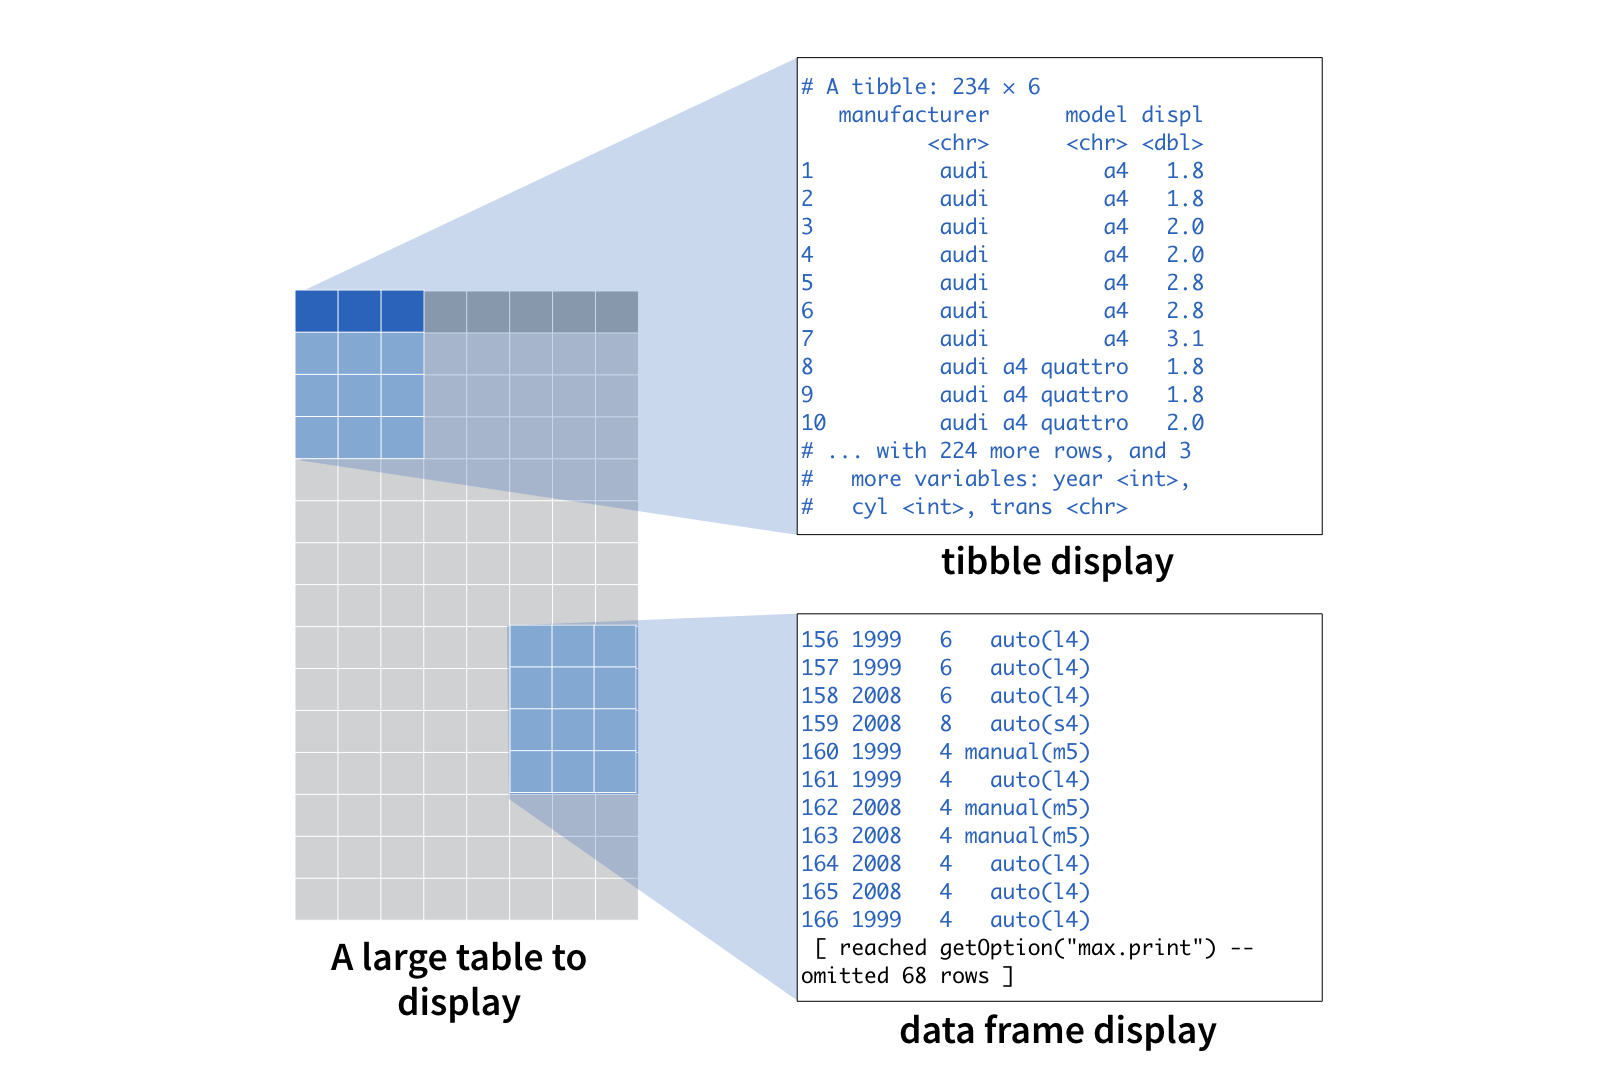
\includegraphics{./data/tibble_display.png} \#\#\#\# as\_tibble()

You can transform a data frame to a tibble with the as\_tibble()
function in the tibble package, e.g.~as\_tibble(cars). However,
babynames is already a tibble. To display it nicely, you just need to
load the tibble package.

To see what I mean, use library() to load the tibble package in the
chunk below and then call babynames.

\begin{Shaded}
\begin{Highlighting}[]
\FunctionTok{library}\NormalTok{(tibble)}
\NormalTok{babynames}
\end{Highlighting}
\end{Shaded}

\begin{verbatim}
## # A tibble: 1,924,665 x 5
##     year sex   name          n   prop
##    <dbl> <chr> <chr>     <int>  <dbl>
##  1  1880 F     Mary       7065 0.0724
##  2  1880 F     Anna       2604 0.0267
##  3  1880 F     Emma       2003 0.0205
##  4  1880 F     Elizabeth  1939 0.0199
##  5  1880 F     Minnie     1746 0.0179
##  6  1880 F     Margaret   1578 0.0162
##  7  1880 F     Ida        1472 0.0151
##  8  1880 F     Alice      1414 0.0145
##  9  1880 F     Bertha     1320 0.0135
## 10  1880 F     Sarah      1288 0.0132
## # ... with 1,924,655 more rows
\end{verbatim}

\begin{verbatim}
"Excellent! If you want to check whether or not an object is a tibble, you can use the `is_tibble()` function that comes in the tibble package. For example, this would return TRUE: `is_tibble(babynames)`."
\end{verbatim}

You do not need to worry much about tibbles in these tutorials; in
future tutorials, I'll automatically convert each data frame into an
interactive table. However, you should consider making tibbles an
important part of your work in R.

\hypertarget{view}{%
\paragraph{View()}\label{view}}

What if you'd like to inspect the remaining portions of a tibble? To see
the entire tibble, use the View() command. R will launch a window that
shows a scrollable display of the entire data set. For example, the code
below will launch a data viewer in the RStudio IDE.

\begin{verbatim}
View(babynames)
\end{verbatim}

View() works in conjunction with the software that you run R from:
View() opens the data editor provided by that software. Unfortunately,
this tutorial doesn't come with a data editor, so you won't be able to
use View() today (unless you open the RStudio IDE, for example, and run
the code there).

\hypertarget{tidyverse}{%
\subsubsection{tidyverse}\label{tidyverse}}

\hypertarget{the-tidyverse}{%
\paragraph{The tidyverse}\label{the-tidyverse}}

The tibble package is one of several packages that are known
collectively as ``\href{http://tidyverse.org/}{the tidyverse}''.
Tidyverse packages share a common philosophy and are designed to work
well together. For example, in this tutorial you will use the tibble
package, the ggplot2 package, and the dplyr package, all of which belong
to the tidyverse.

\hypertarget{the-tidyverse-package}{%
\paragraph{The tidyverse package}\label{the-tidyverse-package}}

When you use tidyverse packages, you can make your life easier by using
the tidyverse package. The tidyverse package provides a shortcut for
installing and loading the entire suite of packages in ``the
tidyverse'', e.g.~

\hypertarget{installing-the-tidyverse}{%
\paragraph{Installing the tidyverse}\label{installing-the-tidyverse}}

Think of the tidyverse package as a placeholder for the packages that
are in the ``tidyverse''. By itself, tidyverse does not do much, but
when you install the tidyverse package it instructs R to install every
other package in the tidyverse at the same time. In other words, when
you run install.packages(``tidyverse''), R installs the following
packages for you in one simple step:

\begin{itemize}
\tightlist
\item
  ggplot2
\item
  dplyr
\item
  tidyr
\item
  readr
\item
  purrr
\item
  tibble
\item
  hms
\item
  stringr
\item
  lubridate
\item
  forcats
\item
  DBI
\item
  haven
\item
  jsonlite
\item
  readxl
\item
  rvest
\item
  xml2
\item
  modelr
\item
  broom
\end{itemize}

\hypertarget{loading-the-tidyverse}{%
\paragraph{loading the tidyverse}\label{loading-the-tidyverse}}

When you load tidyverse with library(``tidyverse''), it instructs R to
load the most commonly used tidyverse packages. These are:

\begin{itemize}
\tightlist
\item
  ggplot2
\item
  dplyr
\item
  tidyr
\item
  readr
\item
  purrr
\item
  tibble
\end{itemize}

You can load the less commonly used tidyverse packages in the normal
way, by running library() for each of them.

Let's give this a try. We will use the ggplot2 and dplyr packages later
in this tutorial. Let's use the tidyverse package to load them in the
chunk below:

\begin{Shaded}
\begin{Highlighting}[]
\FunctionTok{library}\NormalTok{(tidyverse)}
\end{Highlighting}
\end{Shaded}

\hypertarget{quiz}{%
\paragraph{Quiz}\label{quiz}}

Which package is not loaded by library(``tidyverse'')

\begin{itemize}
\tightlist
\item[$\square$]
  ggplot2 ✗
\item[$\square$]
  dplyr ✗
\item[$\square$]
  tibble ✗
\item[$\boxtimes$]
  babynames
\end{itemize}

\begin{verbatim}
Correct! 

Now that you are familiar with the data set, and have loaded the necessary packages, let's explore the data.
\end{verbatim}

\hypertarget{recap-1}{%
\paragraph{Recap}\label{recap-1}}

Tibbles and the tidyverse package are two tools that make life with R
easier. Ironically, you may not come to appreciate their value right
away: these tutorials pre-load packages for you, and they wrap data
frames into an interactive table for display (at least the tutorials in
the primers that follow will). However, you will want to utilize tibbles
and the tidyverse package when you move out of the tutorials and begin
doing your own work with R inside of the RStudio IDE.

This tutorial also introduced the babynames dataset. In the next
tutorial, you will use this data set to plot the popularity of your name
over time. Along the way, you will learn how to filter and subset data
sets in R.

\hypertarget{isolating-data-with-dplyr}{%
\subsection{Isolating Data with dplyr}\label{isolating-data-with-dplyr}}

Master three simple functions for finding, and extracting, the data in
your data set. Here you will learn to select variables, filter
observations, and arrange values. Here, you will also meet R's pipe
operator, \%\textgreater\%.

\hypertarget{welcome-3}{%
\subsubsection{Welcome}\label{welcome-3}}

In this case study, you will explore the popularity of your own name
over time. Along the way, you will master some of the most useful
functions for isolating variables, cases, and values within a data
frame:

\begin{itemize}
\tightlist
\item
  select() and filter(), which let you extract rows and columns from a
  data frame
\item
  arrange(), which lets you reorder the rows in your data
\item
  \%\textgreater\%, which organizes your code into reader-friendly
  ``pipes''
\end{itemize}

This tutorial uses the \href{http://tidyverse.org/}{core tidyverse
packages}, including ggplot2, tibble, and dplyr, as well as the
babynames package. All of these packages have been pre-installed and
pre-loaded for your convenience.

Click the Next Topic button to begin.

\hypertarget{your-name}{%
\subsubsection{Your name}\label{your-name}}

The history of your name

You can use the data in babynames to make graphs like this, which reveal
the history of a name, perhaps your name.

\includegraphics{./data/unnamed-chunk-2-4-1.png} But before you do, you
will need to trim down babynames. At the moment, there are more rows in
babynames than you need to build your plot.

\hypertarget{an-example}{%
\paragraph{An example}\label{an-example}}

To see what I mean, consider how I made the plot above: I began with the
entire data set, which if plotted as a scatterplot would've looked like
this.

\includegraphics{./data/unnamed-chunk-2-5-1.png} I then narrowed the
data to just the rows that contain my name, before plotting the data
with a line geom. Here's how the rows with just my name look as a
scatterplot.

\includegraphics{./data/unnamed-chunk-2-6-1.png} If I had skipped this
step, my line graph would've connected all of the points in the large
data set, creating an uninformative graph.

\includegraphics{./data/unnamed-chunk-2-7-1.png} Your goal in this
section is to repeat this process for your own name (or a name that you
choose). Along the way, you will learn a set of functions that isolate
information within a data set.

\hypertarget{isolating-data}{%
\paragraph{Isolating data}\label{isolating-data}}

This type of task occurs often in Data Science: you need to extract data
from a table before you can use it. You can do this task quickly with
three functions that come in the dplyr package:

\begin{itemize}
\tightlist
\item
  select() - which extracts columns from a data frame
\item
  filter() - which extracts rows from a data frame
\item
  arrange() - which moves important rows to the top of a data frame
\end{itemize}

Each function takes a data frame or tibble as it's first argument and
returns a new data frame or tibble as its output.

\hypertarget{select}{%
\subsubsection{select()}\label{select}}

select() extracts columns of a data frame and returns the columns as a
new data frame. To use select(), pass it the name of a data frame to
extract columns from, and then the names of the columns to extract. The
column names do not need to appear in quotation marks or be prefixed
with a \$; select() knows to find them in the data frame that you
supply.

\hypertarget{exercise---select}{%
\paragraph{Exercise - select()}\label{exercise---select}}

Use the example below to get a feel for select(). Can you extract just
the name column? How about the name and year columns? How about all of
the columns except prop?

\begin{Shaded}
\begin{Highlighting}[]
\FunctionTok{select}\NormalTok{(babynames, name, sex)}
\end{Highlighting}
\end{Shaded}

\begin{verbatim}
## # A tibble: 1,924,665 x 2
##    name      sex  
##    <chr>     <chr>
##  1 Mary      F    
##  2 Anna      F    
##  3 Emma      F    
##  4 Elizabeth F    
##  5 Minnie    F    
##  6 Margaret  F    
##  7 Ida       F    
##  8 Alice     F    
##  9 Bertha    F    
## 10 Sarah     F    
## # ... with 1,924,655 more rows
\end{verbatim}

\begin{Shaded}
\begin{Highlighting}[]
\CommentTok{\# Can you extract just the name column?}
\FunctionTok{select}\NormalTok{(babynames, name)}
\end{Highlighting}
\end{Shaded}

\begin{verbatim}
## # A tibble: 1,924,665 x 1
##    name     
##    <chr>    
##  1 Mary     
##  2 Anna     
##  3 Emma     
##  4 Elizabeth
##  5 Minnie   
##  6 Margaret 
##  7 Ida      
##  8 Alice    
##  9 Bertha   
## 10 Sarah    
## # ... with 1,924,655 more rows
\end{verbatim}

\begin{Shaded}
\begin{Highlighting}[]
\CommentTok{\# How about the name and year columns?}
\FunctionTok{select}\NormalTok{(babynames, name, year)}
\end{Highlighting}
\end{Shaded}

\begin{verbatim}
## # A tibble: 1,924,665 x 2
##    name       year
##    <chr>     <dbl>
##  1 Mary       1880
##  2 Anna       1880
##  3 Emma       1880
##  4 Elizabeth  1880
##  5 Minnie     1880
##  6 Margaret   1880
##  7 Ida        1880
##  8 Alice      1880
##  9 Bertha     1880
## 10 Sarah      1880
## # ... with 1,924,655 more rows
\end{verbatim}

\begin{Shaded}
\begin{Highlighting}[]
\CommentTok{\# How about all of the columns except prop?}
\FunctionTok{select}\NormalTok{(babynames, }\SpecialCharTok{{-}}\NormalTok{prop)}
\end{Highlighting}
\end{Shaded}

\begin{verbatim}
## # A tibble: 1,924,665 x 4
##     year sex   name          n
##    <dbl> <chr> <chr>     <int>
##  1  1880 F     Mary       7065
##  2  1880 F     Anna       2604
##  3  1880 F     Emma       2003
##  4  1880 F     Elizabeth  1939
##  5  1880 F     Minnie     1746
##  6  1880 F     Margaret   1578
##  7  1880 F     Ida        1472
##  8  1880 F     Alice      1414
##  9  1880 F     Bertha     1320
## 10  1880 F     Sarah      1288
## # ... with 1,924,655 more rows
\end{verbatim}

\hypertarget{select-helpers}{%
\paragraph{select() helpers}\label{select-helpers}}

You can also use a series of helpers with select(). For example, if you
place a minus sign before a column name, select() will return every
column but that column. Can you predict how the minus sign will work
here?

\begin{Shaded}
\begin{Highlighting}[]
\FunctionTok{select}\NormalTok{(babynames, }\SpecialCharTok{{-}}\FunctionTok{c}\NormalTok{(n, prop))}
\end{Highlighting}
\end{Shaded}

\begin{verbatim}
## # A tibble: 1,924,665 x 3
##     year sex   name     
##    <dbl> <chr> <chr>    
##  1  1880 F     Mary     
##  2  1880 F     Anna     
##  3  1880 F     Emma     
##  4  1880 F     Elizabeth
##  5  1880 F     Minnie   
##  6  1880 F     Margaret 
##  7  1880 F     Ida      
##  8  1880 F     Alice    
##  9  1880 F     Bertha   
## 10  1880 F     Sarah    
## # ... with 1,924,655 more rows
\end{verbatim}

The table below summarizes the other select() helpers that are available
in dplyr. Study it, and then click ``Continue'' to test your
understanding.

\begin{longtable}[]{@{}
  >{\raggedright\arraybackslash}p{(\columnwidth - 4\tabcolsep) * \real{0.1667}}
  >{\raggedright\arraybackslash}p{(\columnwidth - 4\tabcolsep) * \real{0.3889}}
  >{\raggedright\arraybackslash}p{(\columnwidth - 4\tabcolsep) * \real{0.4444}}@{}}
\toprule()
\begin{minipage}[b]{\linewidth}\raggedright
Helper Function
\end{minipage} & \begin{minipage}[b]{\linewidth}\raggedright
Use
\end{minipage} & \begin{minipage}[b]{\linewidth}\raggedright
Example
\end{minipage} \\
\midrule()
\endhead
- & Columns except & select(babynames, -prop) \\
: & Columns between (inclusive) & select(babynames, year:n) \\
contains() & Columns that contains a string & select(babynames,
contains(``n'')) \\
ends\_with() & Columns that ends with a string & select(babynames,
ends\_with(``n'')) \\
matches() & Columns that matches a regex & select(babynames,
matches(``n'')) \\
num\_range() & Columns with a numerical suffix in the range & Not
applicable with babynames \\
one\_of() & Columns whose name appear in the given set &
select(babynames, one\_of(c(``sex'', ``gender''))) \\
starts\_with() & Columns that starts with a string & select(babynames,
starts\_with(``n'')) \\
\bottomrule()
\end{longtable}

\hypertarget{select-quiz}{%
\paragraph{select() quiz}\label{select-quiz}}

Which of these is not a way to select the name and n columns together?

\begin{itemize}
\tightlist
\item[$\square$]
  select(babynames, -c(year, sex, prop)) ✗
\item[$\square$]
  select(babynames, name:n) ✗
\item[$\square$]
  select(babynames, starts\_with(``n'')) ✗
\item[$\boxtimes$]
  select(babynames, ends\_with(``n'')) ✓
\end{itemize}

\hypertarget{filter}{%
\subsubsection{filter()}\label{filter}}

filter() extracts rows from a data frame and returns them as a new data
frame. As with select(), the first argument of filter() should be a data
frame to extract rows from. The arguments that follow should be logical
tests; filter() will return every row for which the tests return TRUE.

\hypertarget{filter-in-action}{%
\paragraph{filter in action}\label{filter-in-action}}

For example, the code chunk below returns every row with the name
``Sea'' in babynames.

\begin{Shaded}
\begin{Highlighting}[]
\FunctionTok{filter}\NormalTok{(babynames, name }\SpecialCharTok{==} \StringTok{"Sea"}\NormalTok{)}
\end{Highlighting}
\end{Shaded}

\begin{verbatim}
## # A tibble: 4 x 5
##    year sex   name      n       prop
##   <dbl> <chr> <chr> <int>      <dbl>
## 1  1982 F     Sea       5 0.00000276
## 2  1985 M     Sea       6 0.00000312
## 3  1986 M     Sea       5 0.0000026 
## 4  1998 F     Sea       5 0.00000258
\end{verbatim}

\hypertarget{logical-tests}{%
\paragraph{Logical tests}\label{logical-tests}}

To get the most from filter, you will need to know how to use R's
logical test operators, which are summarised below.

\begin{longtable}[]{@{}lll@{}}
\toprule()
Logical operator & tests & Example \\
\midrule()
\endhead
\textgreater{} & Is x greater than y? & x \textgreater{} y \\
\textgreater= & Is x greater than or equal to y? & x \textgreater= y \\
\textless{} & Is x less than y? & x \textless{} y \\
\textless= & Is x less than or equal to y? & x \textless= y \\
== & Is x equal to y? & x == y \\
!= & Is x not equal to y? & x != y \\
is.na() & Is x an NA? & is.na(x) \\
!is.na() & Is x not an NA? & !is.na(x) \\
\bottomrule()
\end{longtable}

\hypertarget{exercise---logical-operators}{%
\paragraph{Exercise - Logical
Operators}\label{exercise---logical-operators}}

See if you can use the logical operators to manipulate our code below to
show:

\begin{itemize}
\tightlist
\item
  All of the names where prop is greater than or equal to 0.08
\item
  All of the children named ``Khaleesi''
\item
  All of the names that have a missing value for n (Hint: this should
  return an empty data set).
\end{itemize}

\begin{Shaded}
\begin{Highlighting}[]
\FunctionTok{filter}\NormalTok{(babynames, name }\SpecialCharTok{==} \StringTok{"Sea"}\NormalTok{)}
\end{Highlighting}
\end{Shaded}

\begin{verbatim}
## # A tibble: 4 x 5
##    year sex   name      n       prop
##   <dbl> <chr> <chr> <int>      <dbl>
## 1  1982 F     Sea       5 0.00000276
## 2  1985 M     Sea       6 0.00000312
## 3  1986 M     Sea       5 0.0000026 
## 4  1998 F     Sea       5 0.00000258
\end{verbatim}

\hypertarget{two-common-mistakes}{%
\paragraph{Two common mistakes}\label{two-common-mistakes}}

When you use logical tests, be sure to look out for two common mistakes.
One appears in each code chunk below. Can you find them? When you spot a
mistake, fix it and then run the chunk to confirm that it works.

\begin{verbatim}
filter(babynames, name = "Sea")
\end{verbatim}

\begin{Shaded}
\begin{Highlighting}[]
\FunctionTok{filter}\NormalTok{(babynames, name }\SpecialCharTok{==} \StringTok{"Sea"}\NormalTok{)}
\end{Highlighting}
\end{Shaded}

\begin{verbatim}
## # A tibble: 4 x 5
##    year sex   name      n       prop
##   <dbl> <chr> <chr> <int>      <dbl>
## 1  1982 F     Sea       5 0.00000276
## 2  1985 M     Sea       6 0.00000312
## 3  1986 M     Sea       5 0.0000026 
## 4  1998 F     Sea       5 0.00000258
\end{verbatim}

\begin{verbatim}
"Good Job! Remember to use == instead of = when testing for equality."
\end{verbatim}

\begin{verbatim}
filter(babynames, name == Sea)
\end{verbatim}

\begin{Shaded}
\begin{Highlighting}[]
\FunctionTok{filter}\NormalTok{(babynames, name }\SpecialCharTok{==} \StringTok{"Sea"}\NormalTok{)}
\end{Highlighting}
\end{Shaded}

\begin{verbatim}
## # A tibble: 4 x 5
##    year sex   name      n       prop
##   <dbl> <chr> <chr> <int>      <dbl>
## 1  1982 F     Sea       5 0.00000276
## 2  1985 M     Sea       6 0.00000312
## 3  1986 M     Sea       5 0.0000026 
## 4  1998 F     Sea       5 0.00000258
\end{verbatim}

\begin{verbatim}
"Good Job! As written this code would check that name is equal to the contents of the object named Sea, which does not exist."
\end{verbatim}

\hypertarget{two-mistakes---recap}{%
\paragraph{Two mistakes - Recap}\label{two-mistakes---recap}}

When you use logical tests, be sure to look out for these two common
mistakes:

\begin{enumerate}
\def\labelenumi{\arabic{enumi}.}
\tightlist
\item
  using = instead of == to test for equality.
\item
  forgetting to use quotation marks when comparing strings, e.g.~name ==
  Abby, instead of name == ``Abby''
\end{enumerate}

\hypertarget{combining-tests}{%
\paragraph{Combining tests}\label{combining-tests}}

If you provide more than one test to filter(), filter() will combine the
tests with an and statement (\&): it will only return the rows that
satisfy all of the tests.

To combine multiple tests in a different way, use R's Boolean operators.
For example, the code below will return all of the children named Sea or
Anemone.

\begin{Shaded}
\begin{Highlighting}[]
\FunctionTok{filter}\NormalTok{(babynames, name }\SpecialCharTok{==} \StringTok{"Sea"} \SpecialCharTok{|}\NormalTok{ name }\SpecialCharTok{==} \StringTok{"Anemone"}\NormalTok{)}
\end{Highlighting}
\end{Shaded}

\begin{verbatim}
## # A tibble: 5 x 5
##    year sex   name        n       prop
##   <dbl> <chr> <chr>   <int>      <dbl>
## 1  1982 F     Sea         5 0.00000276
## 2  1985 M     Sea         6 0.00000312
## 3  1986 M     Sea         5 0.0000026 
## 4  1998 F     Sea         5 0.00000258
## 5  2012 F     Anemone     6 0.0000031
\end{verbatim}

\hypertarget{boolean-operators}{%
\paragraph{Boolean operators}\label{boolean-operators}}

You can find a complete list or base R's boolean operators in the table
below.

\begin{longtable}[]{@{}lll@{}}
\toprule()
Boolean operator & represents & Example \\
\midrule()
\endhead
\& & Are both A and B true? & A \& B \\
& Are one or both of A and B true? & A \\
! & Is A not true? & !A \\
xor() & Is one and only one of A and B true? & xor(A, B) \\
\%in\% & Is x in the set of a, b, and c? & x \%in\% c(a, b, c) \\
any() & Are any of A, B, or C true? & any(A, B, C) \\
all() & Are all of A, B, or C true? & all(A, B, C) \\
\bottomrule()
\end{longtable}

\hypertarget{exercise---combining-tests}{%
\paragraph{Exercise - Combining
tests}\label{exercise---combining-tests}}

Use Boolean operators to alter the code chunk below to return only the
rows that contain:

\begin{itemize}
\tightlist
\item
  Girls named Sea
\item
  Names that were used by exactly 5 or 6 children in 1880
\item
  Names that are one of Acura, Lexus, or Yugo
\end{itemize}

\begin{Shaded}
\begin{Highlighting}[]
\FunctionTok{filter}\NormalTok{(babynames, name }\SpecialCharTok{==} \StringTok{"Sea"} \SpecialCharTok{|}\NormalTok{ name }\SpecialCharTok{==} \StringTok{"Anemone"}\NormalTok{)}
\end{Highlighting}
\end{Shaded}

\begin{verbatim}
## # A tibble: 5 x 5
##    year sex   name        n       prop
##   <dbl> <chr> <chr>   <int>      <dbl>
## 1  1982 F     Sea         5 0.00000276
## 2  1985 M     Sea         6 0.00000312
## 3  1986 M     Sea         5 0.0000026 
## 4  1998 F     Sea         5 0.00000258
## 5  2012 F     Anemone     6 0.0000031
\end{verbatim}

\begin{Shaded}
\begin{Highlighting}[]
\CommentTok{\# Girls named Sea}
\FunctionTok{filter}\NormalTok{(babynames, sex }\SpecialCharTok{==} \StringTok{"F"}\NormalTok{, name }\SpecialCharTok{==} \StringTok{"Sea"}\NormalTok{)}
\end{Highlighting}
\end{Shaded}

\begin{verbatim}
## # A tibble: 2 x 5
##    year sex   name      n       prop
##   <dbl> <chr> <chr> <int>      <dbl>
## 1  1982 F     Sea       5 0.00000276
## 2  1998 F     Sea       5 0.00000258
\end{verbatim}

\begin{Shaded}
\begin{Highlighting}[]
\CommentTok{\# Names that were used by exactly 5 or 6 children in 1880}
\FunctionTok{filter}\NormalTok{(babynames, n }\SpecialCharTok{\%in\%} \FunctionTok{c}\NormalTok{(}\DecValTok{5}\NormalTok{,}\DecValTok{6}\NormalTok{))}
\end{Highlighting}
\end{Shaded}

\begin{verbatim}
## # A tibble: 460,006 x 5
##     year sex   name        n      prop
##    <dbl> <chr> <chr>   <int>     <dbl>
##  1  1880 F     Abby        6 0.0000615
##  2  1880 F     Aileen      6 0.0000615
##  3  1880 F     Alba        6 0.0000615
##  4  1880 F     Alda        6 0.0000615
##  5  1880 F     Alla        6 0.0000615
##  6  1880 F     Alverta     6 0.0000615
##  7  1880 F     Ara         6 0.0000615
##  8  1880 F     Ardelia     6 0.0000615
##  9  1880 F     Ardella     6 0.0000615
## 10  1880 F     Arrie       6 0.0000615
## # ... with 459,996 more rows
\end{verbatim}

\begin{Shaded}
\begin{Highlighting}[]
\CommentTok{\# Names that are one of Acura, Lexus, or Yugo}
\FunctionTok{filter}\NormalTok{(babynames, name }\SpecialCharTok{\%in\%} \FunctionTok{c}\NormalTok{(}\StringTok{"Acura"}\NormalTok{, }\StringTok{"Lexus"}\NormalTok{, }\StringTok{"Yugo"}\NormalTok{))}
\end{Highlighting}
\end{Shaded}

\begin{verbatim}
## # A tibble: 57 x 5
##     year sex   name      n       prop
##    <dbl> <chr> <chr> <int>      <dbl>
##  1  1990 F     Lexus    36 0.0000175 
##  2  1990 M     Lexus    12 0.00000558
##  3  1991 F     Lexus   102 0.0000502 
##  4  1991 M     Lexus    16 0.00000755
##  5  1992 F     Lexus   193 0.0000963 
##  6  1992 M     Lexus    25 0.0000119 
##  7  1993 F     Lexus   285 0.000145  
##  8  1993 M     Lexus    30 0.0000145 
##  9  1994 F     Lexus   381 0.000195  
## 10  1994 F     Acura     6 0.00000308
## # ... with 47 more rows
\end{verbatim}

\hypertarget{two-more-common-mistakes}{%
\paragraph{Two more common mistakes}\label{two-more-common-mistakes}}

Logical tests also invite two common mistakes that you should look out
for. Each is displayed in a code chunk below, one produces an error and
the other is needlessly verbose. Diagnose the chunks and then fix the
code.

\begin{verbatim}
filter(babynames, 10 < n < 20)
\end{verbatim}

\begin{Shaded}
\begin{Highlighting}[]
\FunctionTok{filter}\NormalTok{(babynames, }\DecValTok{10} \SpecialCharTok{\textless{}}\NormalTok{ n, n }\SpecialCharTok{\textless{}} \DecValTok{20}\NormalTok{)}
\end{Highlighting}
\end{Shaded}

\begin{verbatim}
## # A tibble: 365,458 x 5
##     year sex   name           n     prop
##    <dbl> <chr> <chr>      <int>    <dbl>
##  1  1880 F     Antoinette    19 0.000195
##  2  1880 F     Clementine    19 0.000195
##  3  1880 F     Edythe        19 0.000195
##  4  1880 F     Harriette     19 0.000195
##  5  1880 F     Libbie        19 0.000195
##  6  1880 F     Lilian        19 0.000195
##  7  1880 F     Lue           19 0.000195
##  8  1880 F     Lutie         19 0.000195
##  9  1880 F     Magdalena     19 0.000195
## 10  1880 F     Meda          19 0.000195
## # ... with 365,448 more rows
\end{verbatim}

\begin{verbatim}
"Good job! You cannot combine two logical tests in R without using a Boolean operator (or at least a comma between filter arguments)."
\end{verbatim}

\begin{verbatim}
filter(babynames, n == 5 | n == 6 | n == 7 | n == 8 | n == 9)
\end{verbatim}

\begin{Shaded}
\begin{Highlighting}[]
\FunctionTok{filter}\NormalTok{(babynames, n }\SpecialCharTok{\%in\%} \DecValTok{5}\SpecialCharTok{:}\DecValTok{9}\NormalTok{)}
\end{Highlighting}
\end{Shaded}

\begin{verbatim}
## # A tibble: 811,195 x 5
##     year sex   name          n      prop
##    <dbl> <chr> <chr>     <int>     <dbl>
##  1  1880 F     Adela         9 0.0000922
##  2  1880 F     Althea        9 0.0000922
##  3  1880 F     Amalia        9 0.0000922
##  4  1880 F     Amber         9 0.0000922
##  5  1880 F     Angelina      9 0.0000922
##  6  1880 F     Annabelle     9 0.0000922
##  7  1880 F     Anner         9 0.0000922
##  8  1880 F     Arie          9 0.0000922
##  9  1880 F     Clarice       9 0.0000922
## 10  1880 F     Corda         9 0.0000922
## # ... with 811,185 more rows
\end{verbatim}

\begin{verbatim}
"Good job! Although the first code works, you should make your code more concise by collapsing multiple or statements into an %in% statement when possible."
\end{verbatim}

\hypertarget{two-more-common-mistakes---recap}{%
\paragraph{Two more common mistakes -
Recap}\label{two-more-common-mistakes---recap}}

When you combine multiple logical tests, be sure to look out for these
two common mistakes:

\begin{enumerate}
\def\labelenumi{\arabic{enumi}.}
\tightlist
\item
  Collapsing multiple logical tests into a single test without using a
  boolean operator
\item
  Using repeated \textbar{} instead of \%in\%, e.g.~x == 1 \textbar{} x
  == 2 \textbar{} x == 3 instead of x \%in\% c(1, 2, 3)
\end{enumerate}

\hypertarget{arrange}{%
\subsubsection{arrange()}\label{arrange}}

arrange() returns all of the rows of a data frame reordered by the
values of a column. As with select(), the first argument of arrange()
should be a data frame and the remaining arguments should be the names
of columns. If you give arrange() a single column name, it will return
the rows of the data frame reordered so that the row with the lowest
value in that column appears first, the row with the second lowest value
appears second, and so on. If the column contains character strings,
arrange() will place them in alphabetical order.

\hypertarget{exercise---arrange}{%
\paragraph{Exercise - arrange()}\label{exercise---arrange}}

Use the code chunk below to arrange babynames by n.~Can you tell what
the smallest value of n is?

\begin{Shaded}
\begin{Highlighting}[]
\FunctionTok{arrange}\NormalTok{(babynames, n)}
\end{Highlighting}
\end{Shaded}

\begin{verbatim}
## # A tibble: 1,924,665 x 5
##     year sex   name          n      prop
##    <dbl> <chr> <chr>     <int>     <dbl>
##  1  1880 F     Adelle        5 0.0000512
##  2  1880 F     Adina         5 0.0000512
##  3  1880 F     Adrienne      5 0.0000512
##  4  1880 F     Albertine     5 0.0000512
##  5  1880 F     Alys          5 0.0000512
##  6  1880 F     Ana           5 0.0000512
##  7  1880 F     Araminta      5 0.0000512
##  8  1880 F     Arthur        5 0.0000512
##  9  1880 F     Birtha        5 0.0000512
## 10  1880 F     Bulah         5 0.0000512
## # ... with 1,924,655 more rows
\end{verbatim}

\begin{verbatim}
"Good job! The compiler of `babynames` used 5 as a cutoff; a name only made it into babynames for a given year and gender if it was used for five or more children."
\end{verbatim}

\hypertarget{tie-breakers}{%
\paragraph{Tie breakers}\label{tie-breakers}}

If you supply additional column names, arrange() will use them as tie
breakers to order rows that have identical values in the earlier
columns. Add to the code below, to make prop a tie breaker. The result
should first order rows by value of n and then reorder rows within each
value of n by values of prop.

\begin{verbatim}
arrange(babynames, n)
\end{verbatim}

\begin{Shaded}
\begin{Highlighting}[]
\FunctionTok{arrange}\NormalTok{(babynames, n, prop)}
\end{Highlighting}
\end{Shaded}

\begin{verbatim}
## # A tibble: 1,924,665 x 5
##     year sex   name            n       prop
##    <dbl> <chr> <chr>       <int>      <dbl>
##  1  2007 M     Aaban           5 0.00000226
##  2  2007 M     Aareon          5 0.00000226
##  3  2007 M     Aaris           5 0.00000226
##  4  2007 M     Abd             5 0.00000226
##  5  2007 M     Abdulazeez      5 0.00000226
##  6  2007 M     Abdulhadi       5 0.00000226
##  7  2007 M     Abdulhamid      5 0.00000226
##  8  2007 M     Abdulkadir      5 0.00000226
##  9  2007 M     Abdulraheem     5 0.00000226
## 10  2007 M     Abdulrahim      5 0.00000226
## # ... with 1,924,655 more rows
\end{verbatim}

\hypertarget{desc}{%
\paragraph{desc}\label{desc}}

If you would rather arrange rows in the opposite order, i.e.~from large
values to small values, surround a column name with desc(). arrange()
will reorder the rows based on the largest values to the smallest.

Add a desc() to the code below to display the most popular name for 2017
(the largest year in the dataset) instead of 1880 (the smallest year in
the dataset).

\begin{verbatim}
arrange(babynames, year, desc(prop))
\end{verbatim}

\begin{Shaded}
\begin{Highlighting}[]
\FunctionTok{arrange}\NormalTok{(babynames, }\FunctionTok{desc}\NormalTok{(year), }\FunctionTok{desc}\NormalTok{(n))}
\end{Highlighting}
\end{Shaded}

\begin{verbatim}
## # A tibble: 1,924,665 x 5
##     year sex   name         n    prop
##    <dbl> <chr> <chr>    <int>   <dbl>
##  1  2017 F     Emma     19738 0.0105 
##  2  2017 M     Liam     18728 0.00954
##  3  2017 F     Olivia   18632 0.00994
##  4  2017 M     Noah     18326 0.00933
##  5  2017 F     Ava      15902 0.00848
##  6  2017 F     Isabella 15100 0.00805
##  7  2017 M     William  14904 0.00759
##  8  2017 F     Sophia   14831 0.00791
##  9  2017 M     James    14232 0.00725
## 10  2017 M     Logan    13974 0.00712
## # ... with 1,924,655 more rows
\end{verbatim}

Think you have it? Click Continue to test yourself.

\hypertarget{arrange-quiz}{%
\paragraph{arrange() quiz}\label{arrange-quiz}}

Which name was the most popular for a single gender in a single year? In
the code chunk below, use arrange() to make the row with the largest
value of prop appear at the top of the data set.

\begin{Shaded}
\begin{Highlighting}[]
\FunctionTok{arrange}\NormalTok{(babynames, }\FunctionTok{desc}\NormalTok{(prop))}
\end{Highlighting}
\end{Shaded}

\begin{verbatim}
## # A tibble: 1,924,665 x 5
##     year sex   name        n   prop
##    <dbl> <chr> <chr>   <int>  <dbl>
##  1  1880 M     John     9655 0.0815
##  2  1881 M     John     8769 0.0810
##  3  1880 M     William  9532 0.0805
##  4  1883 M     John     8894 0.0791
##  5  1881 M     William  8524 0.0787
##  6  1882 M     John     9557 0.0783
##  7  1884 M     John     9388 0.0765
##  8  1882 M     William  9298 0.0762
##  9  1886 M     John     9026 0.0758
## 10  1885 M     John     8756 0.0755
## # ... with 1,924,655 more rows
\end{verbatim}

\begin{Shaded}
\begin{Highlighting}[]
\FunctionTok{arrange}\NormalTok{(babynames, }\FunctionTok{desc}\NormalTok{(n))}
\end{Highlighting}
\end{Shaded}

\begin{verbatim}
## # A tibble: 1,924,665 x 5
##     year sex   name        n   prop
##    <dbl> <chr> <chr>   <int>  <dbl>
##  1  1947 F     Linda   99686 0.0548
##  2  1948 F     Linda   96209 0.0552
##  3  1947 M     James   94756 0.0510
##  4  1957 M     Michael 92695 0.0424
##  5  1947 M     Robert  91642 0.0493
##  6  1949 F     Linda   91016 0.0518
##  7  1956 M     Michael 90620 0.0423
##  8  1958 M     Michael 90520 0.0420
##  9  1948 M     James   88588 0.0497
## 10  1954 M     Michael 88514 0.0428
## # ... with 1,924,655 more rows
\end{verbatim}

\begin{verbatim}
"The number of children represented by each proportion grew over time as the population grew."
\end{verbatim}

\hypertarget{section}{%
\subsubsection{\%\textgreater\%}\label{section}}

\hypertarget{steps}{%
\paragraph{Steps}\label{steps}}

Notice how each dplyr function takes a data frame as input and returns a
data frame as output. This makes the functions easy to use in a step by
step fashion. For example, you could:

\begin{enumerate}
\def\labelenumi{\arabic{enumi}.}
\tightlist
\item
  Filter babynames to just boys born in 2017
\item
  Select the name and n columns from the result
\item
  Arrange those columns so that the most popular names appear near the
  top.
\end{enumerate}

\begin{Shaded}
\begin{Highlighting}[]
\NormalTok{boys\_2017 }\OtherTok{\textless{}{-}} \FunctionTok{filter}\NormalTok{(babynames, year }\SpecialCharTok{==} \DecValTok{2017}\NormalTok{, sex }\SpecialCharTok{==} \StringTok{"M"}\NormalTok{)}
\NormalTok{boys\_2017 }\OtherTok{\textless{}{-}} \FunctionTok{select}\NormalTok{(boys\_2017, name, n)}
\NormalTok{boys\_2017 }\OtherTok{\textless{}{-}} \FunctionTok{arrange}\NormalTok{(boys\_2017, }\FunctionTok{desc}\NormalTok{(n))}
\NormalTok{boys\_2017}
\end{Highlighting}
\end{Shaded}

\begin{verbatim}
## # A tibble: 14,160 x 2
##    name         n
##    <chr>    <int>
##  1 Liam     18728
##  2 Noah     18326
##  3 William  14904
##  4 James    14232
##  5 Logan    13974
##  6 Benjamin 13733
##  7 Mason    13502
##  8 Elijah   13268
##  9 Oliver   13141
## 10 Jacob    13106
## # ... with 14,150 more rows
\end{verbatim}

\hypertarget{redundancy}{%
\paragraph{Redundancy}\label{redundancy}}

The result shows us the most popular boys names from 2017, which is the
most recent year in the data set. But take a look at the code. Do you
notice how we re-create boys\_2017 at each step so we will have
something to pass to the next step? This is an inefficient way to write
R code.

You could avoid creating boys\_2017 by nesting your functions inside of
each other, but this creates code that is hard to read:

\begin{Shaded}
\begin{Highlighting}[]
\FunctionTok{arrange}\NormalTok{(}\FunctionTok{select}\NormalTok{(}\FunctionTok{filter}\NormalTok{(babynames, year }\SpecialCharTok{==} \DecValTok{2017}\NormalTok{, sex }\SpecialCharTok{==} \StringTok{"M"}\NormalTok{), name, n), }\FunctionTok{desc}\NormalTok{(n))}
\end{Highlighting}
\end{Shaded}

\begin{verbatim}
## # A tibble: 14,160 x 2
##    name         n
##    <chr>    <int>
##  1 Liam     18728
##  2 Noah     18326
##  3 William  14904
##  4 James    14232
##  5 Logan    13974
##  6 Benjamin 13733
##  7 Mason    13502
##  8 Elijah   13268
##  9 Oliver   13141
## 10 Jacob    13106
## # ... with 14,150 more rows
\end{verbatim}

The dplyr package provides a third way to write sequences of functions:
the pipe.

\hypertarget{section-1}{%
\paragraph{\%\textgreater\%}\label{section-1}}

The pipe operator \%\textgreater\% performs an extremely simple task: it
passes the result on its left into the first argument of the function on
its right. Or put another way, x \%\textgreater\% f(y) is the same as
f(x, y). This piece of code punctuation makes it easy to write and read
series of functions that are applied in a step by step way. For example,
we can use the pipe to rewrite our code above:

\begin{Shaded}
\begin{Highlighting}[]
\NormalTok{babynames }\SpecialCharTok{\%\textgreater{}\%} 
  \FunctionTok{filter}\NormalTok{(year }\SpecialCharTok{==} \DecValTok{2017}\NormalTok{, sex }\SpecialCharTok{==} \StringTok{"M"}\NormalTok{) }\SpecialCharTok{\%\textgreater{}\%} 
  \FunctionTok{select}\NormalTok{(name, n) }\SpecialCharTok{\%\textgreater{}\%} 
  \FunctionTok{arrange}\NormalTok{(}\FunctionTok{desc}\NormalTok{(n))}
\end{Highlighting}
\end{Shaded}

\begin{verbatim}
## # A tibble: 14,160 x 2
##    name         n
##    <chr>    <int>
##  1 Liam     18728
##  2 Noah     18326
##  3 William  14904
##  4 James    14232
##  5 Logan    13974
##  6 Benjamin 13733
##  7 Mason    13502
##  8 Elijah   13268
##  9 Oliver   13141
## 10 Jacob    13106
## # ... with 14,150 more rows
\end{verbatim}

As you read the code, pronounce \%\textgreater\% as ``then''. You'll
notice that dplyr makes it easy to read pipes. Each function name is a
verb, so our code resembles the statement, ``Take babynames, then filter
it by name and sex, then select the name and n columns, then arrange the
results by descending values of n.''

dplyr also makes it easy to write pipes. Each dplyr function returns a
data frame that can be piped into another dplyr function, which will
accept the data frame as its first argument. In fact, dplyr functions
are written with pipes in mind: each function does one simple task.
dplyr expects you to use pipes to combine these simple tasks to produce
sophisticated results.

\hypertarget{exercise---pipes}{%
\paragraph{Exercise - Pipes}\label{exercise---pipes}}

I'll use pipes for the remainder of the tutorial, and I will expect you
to as well. Let's practice a little by writing a new pipe in the chunk
below. The pipe should:

\begin{enumerate}
\def\labelenumi{\arabic{enumi}.}
\tightlist
\item
  Filter babynames to just the girls that were born in 2017
\item
  Select the name and n columns
\item
  Arrange the results so that the most popular names are near the top.
\end{enumerate}

Try to write your pipe without copying and pasting the code from above.

\begin{Shaded}
\begin{Highlighting}[]
\NormalTok{babynames }\SpecialCharTok{\%\textgreater{}\%} 
  \FunctionTok{filter}\NormalTok{(year }\SpecialCharTok{==} \DecValTok{2017}\NormalTok{, sex }\SpecialCharTok{==} \StringTok{"F"}\NormalTok{) }\SpecialCharTok{\%\textgreater{}\%} 
  \FunctionTok{select}\NormalTok{(name, n) }\SpecialCharTok{\%\textgreater{}\%} 
  \FunctionTok{arrange}\NormalTok{(}\FunctionTok{desc}\NormalTok{(n))}
\end{Highlighting}
\end{Shaded}

\begin{verbatim}
## # A tibble: 18,309 x 2
##    name          n
##    <chr>     <int>
##  1 Emma      19738
##  2 Olivia    18632
##  3 Ava       15902
##  4 Isabella  15100
##  5 Sophia    14831
##  6 Mia       13437
##  7 Charlotte 12893
##  8 Amelia    11800
##  9 Evelyn    10675
## 10 Abigail   10551
## # ... with 18,299 more rows
\end{verbatim}

\hypertarget{your-name-1}{%
\paragraph{Your name}\label{your-name-1}}

You've now mastered a set of skills that will let you easily plot the
popularity of your name over time. In the code chunk below, use a
combination of dplyr and ggplot2 functions with \%\textgreater\% to:

\begin{enumerate}
\def\labelenumi{\arabic{enumi}.}
\tightlist
\item
  Trim babynames to just the rows that contain your name and your sex
\item
  Trim the result to just the columns that will appear in your graph
  (not strictly necessary, but useful practice)
\item
  Plot the results as a line graph with year on the x axis and prop on
  the y axis
\end{enumerate}

Note that the first argument of ggplot() takes a data frame, which means
you can add ggplot() directly to the end of a pipe. However, you will
need to switch from \%\textgreater\% to + to finish adding layers to
your plot.

\begin{Shaded}
\begin{Highlighting}[]
\NormalTok{babynames }\SpecialCharTok{\%\textgreater{}\%} 
   \FunctionTok{filter}\NormalTok{(name }\SpecialCharTok{==} \StringTok{"John"}\NormalTok{, sex }\SpecialCharTok{==} \StringTok{"M"}\NormalTok{) }\SpecialCharTok{\%\textgreater{}\%}
   \FunctionTok{select}\NormalTok{(year, prop) }\SpecialCharTok{\%\textgreater{}\%}
   \FunctionTok{ggplot}\NormalTok{() }\SpecialCharTok{+}
      \FunctionTok{geom\_line}\NormalTok{(}\FunctionTok{aes}\NormalTok{(}\AttributeTok{x =}\NormalTok{ year, }\AttributeTok{y =}\NormalTok{ prop))}
\end{Highlighting}
\end{Shaded}

\includegraphics{rstudio_primers_files/figure-latex/unnamed-chunk-74-1.pdf}
\#\#\#\# Recap

Together, select(), filter(), and arrange() let you quickly find
information displayed within your data.

The next tutorial will show you how to derive information that is
implied by your data, but not displayed within your data set.

In that tutorial, you will continue to use the \%\textgreater\%
operator, which is an essential part of programming with the dplyr
library.

Pipes help make R expressive, like a spoken language. Spoken languages
consist of simple words that you combine into sentences to create
sophisticated thoughts.

In the tidyverse, functions are like words: each does one simple task
well. You can combine these tasks into pipes with \%\textgreater\% to
perform complex, customized procedures.

\hypertarget{deriving-information-with-dplyr}{%
\subsection{Deriving Information with
dplyr}\label{deriving-information-with-dplyr}}

Data sets contain more information than they display, and this tutorial
will show you how to access that information. You'll learn to derive new
variables and to compute groupwise summary statistics.

\hypertarget{welcome-4}{%
\subsubsection{Welcome}\label{welcome-4}}

In this case study, you will identify the most popular American names
from 1880 to 2015. While doing this, you will master three more dplyr
functions:

\begin{itemize}
\tightlist
\item
  mutate(), group\_by(), and summarize(), which help you use your data
  to compute new variables and summary statistics
\end{itemize}

These are some of the most useful R functions for data science, and this
tutorial provides everything you need to learn them.

This tutorial uses the \href{http://tidyverse.org/}{core tidyverse
packages}, including ggplot2, tibble, and dplyr, as well as the
babynames package. All of these packages have been pre-installed and
pre-loaded for your convenience.

Click the Next Topic button to begin.

\hypertarget{the-most-popular-names}{%
\subsubsection{The most popular names}\label{the-most-popular-names}}

\hypertarget{what-are-the-most-popular-names-of-all-time}{%
\paragraph{What are the most popular names of all
time?}\label{what-are-the-most-popular-names-of-all-time}}

Let's use babynames to anwser a different question: what are the most
popular names of all time?

This question seems simple enough, but to answer it we need to be more
precise: how do you define ``the most popular'' names? Try to think of
several definitions and then click Continue. After the Continue button,
I will suggest two definitions of my own.

\hypertarget{two-definitions-of-popular}{%
\paragraph{Two definitions of
popular}\label{two-definitions-of-popular}}

I suggest that we focus on two definitions of popular, one that uses
sums and one that uses ranks:

\begin{enumerate}
\def\labelenumi{\arabic{enumi}.}
\tightlist
\item
  Sums - A name is popular if the total number of children that have the
  name is large when you sum across years.
\item
  Ranks - A name is popular if it consistently ranks among the top names
  from year to year.
\end{enumerate}

This raises a question:

Do we have enough information in babynames to compare the popularity of
names?

\begin{itemize}
\tightlist
\item[$\square$]
  No.~No cell in babynames contains a rank value or a sum across years.
  ✗
\item[$\boxtimes$]
  Yes. We can use the information in babynames to compute the values we
  want. ✓
\end{itemize}

\hypertarget{deriving-information}{%
\paragraph{Deriving information}\label{deriving-information}}

Every data frame that you meet implies more information than it
displays. For example, babynames does not display the total number of
children who had your name, but babynames certainly implies what that
number is. To discover the number, you only need to do a calculation:

\begin{Shaded}
\begin{Highlighting}[]
\NormalTok{babynames }\SpecialCharTok{\%\textgreater{}\%} 
  \FunctionTok{filter}\NormalTok{(name }\SpecialCharTok{==} \StringTok{"Garrett"}\NormalTok{, sex }\SpecialCharTok{==} \StringTok{"M"}\NormalTok{) }\SpecialCharTok{\%\textgreater{}\%} 
  \FunctionTok{summarise}\NormalTok{(}\AttributeTok{total =} \FunctionTok{sum}\NormalTok{(n))}
\end{Highlighting}
\end{Shaded}

\begin{verbatim}
## # A tibble: 1 x 1
##    total
##    <int>
## 1 129759
\end{verbatim}

\hypertarget{useful-functions}{%
\paragraph{Useful functions}\label{useful-functions}}

dplyr provides three functions that can help you reveal the information
implied by your data:

\begin{itemize}
\tightlist
\item
  summarise()
\item
  group\_by()
\item
  mutate()
\end{itemize}

Like select(), filter() and arrange(), these functions all take a data
frame as their first argument and return a new data frame as their
output, which makes them easy to use in pipes.

Let's master each function and use them to analyze popularity as we go.

\hypertarget{summarise}{%
\subsubsection{summarise()}\label{summarise}}

summarise() takes a data frame and uses it to calculate a new data frame
of summary statistics.

\hypertarget{syntax}{%
\paragraph{Syntax}\label{syntax}}

To use summarise(), pass it a data frame and then one or more named
arguments. Each named argument should be set to an R expression that
generates a single value. Summarise will turn each named argument into a
column in the new data frame. The name of each argument will become the
column name, and the value returned by the argument will become the
column contents.

\hypertarget{example}{%
\paragraph{Example}\label{example}}

I used summarise() above to calculate the total number of boys named
``Garrett'', but let's expand that code to also calculate

\begin{itemize}
\tightlist
\item
  max - the maximum number of boys named ``Garrett'' in a single year
\item
  mean - the mean number of boys named ``Garrett'' per year
\end{itemize}

\begin{Shaded}
\begin{Highlighting}[]
\NormalTok{babynames }\SpecialCharTok{\%\textgreater{}\%} 
  \FunctionTok{filter}\NormalTok{(name }\SpecialCharTok{==} \StringTok{"Garrett"}\NormalTok{, sex }\SpecialCharTok{==} \StringTok{"M"}\NormalTok{) }\SpecialCharTok{\%\textgreater{}\%} 
  \FunctionTok{summarise}\NormalTok{(}\AttributeTok{total =} \FunctionTok{sum}\NormalTok{(n), }\AttributeTok{max =} \FunctionTok{max}\NormalTok{(n), }\AttributeTok{mean =} \FunctionTok{mean}\NormalTok{(n))}
\end{Highlighting}
\end{Shaded}

\begin{verbatim}
## # A tibble: 1 x 3
##    total   max  mean
##    <int> <int> <dbl>
## 1 129759  5840  940.
\end{verbatim}

Don't let the code above fool you. The first argument of summarise() is
always a data frame, but when you use summarise() in a pipe, the first
argument is provided by the pipe operator, \%\textgreater\%. Here the
first argument will be the data frame that is returned by
\texttt{babynames\ \%\textgreater{}\%\ filter(name\ ==\ "Garrett",\ sex\ ==\ "M")}.

\hypertarget{exercise---summarise}{%
\paragraph{Exercise - summarise()}\label{exercise---summarise}}

Use the code chunk below to compute three statistics:

\begin{enumerate}
\def\labelenumi{\arabic{enumi}.}
\tightlist
\item
  the total number of children who ever had your name
\item
  the maximum number of children given your name in a single year
\item
  the mean number of children given your name per year
\end{enumerate}

If you cannot think of an R function that would compute each statistic,
click the Hint/Solution button.

\begin{Shaded}
\begin{Highlighting}[]
\NormalTok{babynames }\SpecialCharTok{\%\textgreater{}\%} 
  \FunctionTok{filter}\NormalTok{(name }\SpecialCharTok{==} \StringTok{"John"}\NormalTok{, sex }\SpecialCharTok{==} \StringTok{"M"}\NormalTok{) }\SpecialCharTok{\%\textgreater{}\%} 
  \FunctionTok{summarise}\NormalTok{(}\AttributeTok{total =} \FunctionTok{sum}\NormalTok{(n), }\AttributeTok{max =} \FunctionTok{max}\NormalTok{(n), }\AttributeTok{mean =} \FunctionTok{mean}\NormalTok{(n))}
\end{Highlighting}
\end{Shaded}

\begin{verbatim}
## # A tibble: 1 x 3
##     total   max   mean
##     <int> <int>  <dbl>
## 1 5115466 88318 37069.
\end{verbatim}

\hypertarget{summary-functions}{%
\paragraph{Summary functions}\label{summary-functions}}

So far our summarise() examples have relied on sum(), max(), and mean().
But you can use any function in summarise() so long as it meets one
criteria: the function must take a vector of values as input and return
a single value as output. Functions that do this are known as summary
functions and they are common in the field of descriptive statistics.
Some of the most useful summary functions include:

\begin{enumerate}
\def\labelenumi{\arabic{enumi}.}
\tightlist
\item
  Measures of location - mean(x), median(x), quantile(x, 0.25), min(x),
  and max(x)
\item
  Measures of spread - sd(x), var(x), IQR(x), and mad(x)
\item
  Measures of position - first(x), nth(x, 2), and last(x)
\item
  Counts - n\_distinct(x) and n(), which takes no arguments, and returns
  the size of the current group or data frame.
\item
  Counts and proportions of logical values - sum(!is.na(x)), which
  counts the number of TRUEs returned by a logical test; mean(y == 0),
  which returns the proportion of TRUEs returned by a logical test.
\end{enumerate}

Let's apply some of these summary functions. Click Continue to test your
understanding.

\hypertarget{khaleesi-challenge}{%
\paragraph{Khaleesi challenge}\label{khaleesi-challenge}}

``Khaleesi'' is a very modern name that appears to be based on the Game
of Thrones TV series, which premiered on April 17, 2011. In the chunk
below, filter babynames to just the rows where name == ``Khaleesi''.
Then use summarise() and a summary function to return the first value of
year in the data set.

\begin{Shaded}
\begin{Highlighting}[]
\NormalTok{babynames }\SpecialCharTok{\%\textgreater{}\%}
   \FunctionTok{filter}\NormalTok{(name }\SpecialCharTok{==} \StringTok{"Khaleesi"}\NormalTok{) }\SpecialCharTok{\%\textgreater{}\%}
   \FunctionTok{summarize}\NormalTok{(}\AttributeTok{year =} \FunctionTok{first}\NormalTok{(year))}
\end{Highlighting}
\end{Shaded}

\begin{verbatim}
## # A tibble: 1 x 1
##    year
##   <dbl>
## 1  2011
\end{verbatim}

\hypertarget{distinct-name-challenge}{%
\paragraph{Distinct name challenge}\label{distinct-name-challenge}}

In the chunk below, use summarise() and a summary function to return a
data frame with two columns:

\begin{itemize}
\tightlist
\item
  A column named n that displays the total number of rows in babynames
\item
  A column named distinct that displays the number of distinct names in
  babynames
\end{itemize}

Will these numbers be different? Why or why not?

\begin{Shaded}
\begin{Highlighting}[]
\NormalTok{babynames }\SpecialCharTok{\%\textgreater{}\%} 
   \FunctionTok{summarize}\NormalTok{(}\FunctionTok{n}\NormalTok{(), }\AttributeTok{distinct =} \FunctionTok{n\_distinct}\NormalTok{(name))}
\end{Highlighting}
\end{Shaded}

\begin{verbatim}
## # A tibble: 1 x 2
##     `n()` distinct
##     <int>    <int>
## 1 1924665    97310
\end{verbatim}

\begin{verbatim}
"Good job! The two numbers are different because most names appear in the data set more than once. They appear once for each year in which they were used."
\end{verbatim}

\hypertarget{summarise-by-groups}{%
\paragraph{summarise by groups?}\label{summarise-by-groups}}

How can we apply summarise() to find the most popular names in
babynames? You've seen how to calculate the total number of children
that have your name, which provides one of our measures of popularity,
i.e.~the total number of children that have a name:

\begin{verbatim}
babynames %>% 
  filter(name == "Garrett", sex == "M") %>% 
  summarise(total = sum(n))
\end{verbatim}

However, we had to isolate your name from the rest of your data to
calculate this number. You could imagine writing a program that goes
through each name one at a time and:

\begin{enumerate}
\def\labelenumi{\arabic{enumi}.}
\tightlist
\item
  filters out the rows with just that name
\item
  applies summarise to the rows
\end{enumerate}

Eventually, the program could combine all of the results back into a
single data set. However, you don't need to write such a program; this
is the job of dplyr's group\_by() function.

\hypertarget{group_by}{%
\subsubsection{group\_by()}\label{group_by}}

group\_by() takes a data frame and then the names of one or more columns
in the data frame. It returns a copy of the data frame that has been
``grouped'' into sets of rows that share identical combinations of
values in the specified columns.

\hypertarget{group_by-in-action}{%
\paragraph{group\_by() in action}\label{group_by-in-action}}

For example, the result below is grouped into rows that have the same
combination of year and sex values: boys in 1880 are treated as one
group, girls in 1880 as another group and so on.

\begin{Shaded}
\begin{Highlighting}[]
\NormalTok{babynames }\SpecialCharTok{\%\textgreater{}\%}
  \FunctionTok{group\_by}\NormalTok{(year, sex)}
\end{Highlighting}
\end{Shaded}

\begin{verbatim}
## # A tibble: 1,924,665 x 5
## # Groups:   year, sex [276]
##     year sex   name          n   prop
##    <dbl> <chr> <chr>     <int>  <dbl>
##  1  1880 F     Mary       7065 0.0724
##  2  1880 F     Anna       2604 0.0267
##  3  1880 F     Emma       2003 0.0205
##  4  1880 F     Elizabeth  1939 0.0199
##  5  1880 F     Minnie     1746 0.0179
##  6  1880 F     Margaret   1578 0.0162
##  7  1880 F     Ida        1472 0.0151
##  8  1880 F     Alice      1414 0.0145
##  9  1880 F     Bertha     1320 0.0135
## 10  1880 F     Sarah      1288 0.0132
## # ... with 1,924,655 more rows
\end{verbatim}

\hypertarget{using-group_by}{%
\paragraph{Using group\_by()}\label{using-group_by}}

By itself, group\_by() doesn't do much. It assigns grouping criteria
that is stored as metadata alongside the original data set. If your
dataset is a tibble, as above, R will tell you that the data is grouped
at the top of the tibble display. In all other aspects, the data looks
the same.

However, when you apply a dplyr function like summarise() to grouped
data, dplyr will execute the function in a groupwise manner. Instead of
computing a single summary for the entire data set, dplyr will compute
individual summaries for each group and return them as a single data
frame. The data frame will contain the summary columns as well as the
columns in the grouping criteria, which makes the result decipherable:

\begin{Shaded}
\begin{Highlighting}[]
\NormalTok{babynames }\SpecialCharTok{\%\textgreater{}\%}
  \FunctionTok{group\_by}\NormalTok{(year, sex) }\SpecialCharTok{\%\textgreater{}\%} 
  \FunctionTok{summarise}\NormalTok{(}\AttributeTok{total =} \FunctionTok{sum}\NormalTok{(n))}
\end{Highlighting}
\end{Shaded}

\begin{verbatim}
## `summarise()` has grouped output by 'year'. You can override using the
## `.groups` argument.
\end{verbatim}

\begin{verbatim}
## # A tibble: 276 x 3
## # Groups:   year [138]
##     year sex    total
##    <dbl> <chr>  <int>
##  1  1880 F      90993
##  2  1880 M     110491
##  3  1881 F      91953
##  4  1881 M     100743
##  5  1882 F     107847
##  6  1882 M     113686
##  7  1883 F     112319
##  8  1883 M     104627
##  9  1884 F     129020
## 10  1884 M     114442
## # ... with 266 more rows
\end{verbatim}

To understand exactly what group\_by() is doing, remove the line
group\_by(year, sex) \%\textgreater\% from the code above and rerun it.
How do the results change?

\begin{Shaded}
\begin{Highlighting}[]
\NormalTok{babynames }\SpecialCharTok{\%\textgreater{}\%}
  \FunctionTok{summarise}\NormalTok{(}\AttributeTok{total =} \FunctionTok{sum}\NormalTok{(n))}
\end{Highlighting}
\end{Shaded}

\begin{verbatim}
## # A tibble: 1 x 1
##       total
##       <int>
## 1 348120517
\end{verbatim}

\hypertarget{ungrouping-1}{%
\paragraph{Ungrouping 1}\label{ungrouping-1}}

If you apply summarise() to grouped data, summarise() will return data
that is grouped in a similar, but not identical fashion. summarise()
will remove the last variable in the grouping criteria, which creates a
data frame that is grouped at a higher level. For example, this
summarise() statement receives a data frame that is grouped by year and
sex, but it returns a data frame that is grouped only by year.

\begin{Shaded}
\begin{Highlighting}[]
\NormalTok{babynames }\SpecialCharTok{\%\textgreater{}\%}
  \FunctionTok{group\_by}\NormalTok{(year, sex) }\SpecialCharTok{\%\textgreater{}\%} 
  \FunctionTok{summarise}\NormalTok{(}\AttributeTok{total =} \FunctionTok{sum}\NormalTok{(n))}
\end{Highlighting}
\end{Shaded}

\begin{verbatim}
## `summarise()` has grouped output by 'year'. You can override using the
## `.groups` argument.
\end{verbatim}

\begin{verbatim}
## # A tibble: 276 x 3
## # Groups:   year [138]
##     year sex    total
##    <dbl> <chr>  <int>
##  1  1880 F      90993
##  2  1880 M     110491
##  3  1881 F      91953
##  4  1881 M     100743
##  5  1882 F     107847
##  6  1882 M     113686
##  7  1883 F     112319
##  8  1883 M     104627
##  9  1884 F     129020
## 10  1884 M     114442
## # ... with 266 more rows
\end{verbatim}

\hypertarget{ungrouping-2}{%
\paragraph{Ungrouping 2}\label{ungrouping-2}}

If only one grouping variable is left in the grouping criteria,
summarise() will return an ungrouped data set. This feature let's you
progressively ``unwrap'' a grouped data set:

If we add another summarise() to our pipe,

\begin{enumerate}
\def\labelenumi{\arabic{enumi}.}
\tightlist
\item
  our data set will first be grouped by year and sex.
\item
  Then it will be summarised into a data set grouped by year (i.e.~the
  result above)
\item
  Then be summarised into a final data set that is not grouped.
\end{enumerate}

\begin{Shaded}
\begin{Highlighting}[]
\NormalTok{babynames }\SpecialCharTok{\%\textgreater{}\%}
  \FunctionTok{group\_by}\NormalTok{(year, sex) }\SpecialCharTok{\%\textgreater{}\%} 
  \FunctionTok{summarise}\NormalTok{(}\AttributeTok{total =} \FunctionTok{sum}\NormalTok{(n)) }\SpecialCharTok{\%\textgreater{}\%} 
  \FunctionTok{summarise}\NormalTok{(}\AttributeTok{total =} \FunctionTok{sum}\NormalTok{(total))}
\end{Highlighting}
\end{Shaded}

\begin{verbatim}
## `summarise()` has grouped output by 'year'. You can override using the
## `.groups` argument.
\end{verbatim}

\begin{verbatim}
## # A tibble: 138 x 2
##     year  total
##    <dbl>  <int>
##  1  1880 201484
##  2  1881 192696
##  3  1882 221533
##  4  1883 216946
##  5  1884 243462
##  6  1885 240854
##  7  1886 255317
##  8  1887 247394
##  9  1888 299473
## 10  1889 288946
## # ... with 128 more rows
\end{verbatim}

\hypertarget{ungrouping-3}{%
\paragraph{Ungrouping 3}\label{ungrouping-3}}

If you wish to manually remove the grouping criteria from a data set,
you can do so with ungroup().

\begin{Shaded}
\begin{Highlighting}[]
\NormalTok{babynames }\SpecialCharTok{\%\textgreater{}\%}
  \FunctionTok{group\_by}\NormalTok{(year, sex) }\SpecialCharTok{\%\textgreater{}\%} 
  \FunctionTok{ungroup}\NormalTok{()}
\end{Highlighting}
\end{Shaded}

\begin{verbatim}
## # A tibble: 1,924,665 x 5
##     year sex   name          n   prop
##    <dbl> <chr> <chr>     <int>  <dbl>
##  1  1880 F     Mary       7065 0.0724
##  2  1880 F     Anna       2604 0.0267
##  3  1880 F     Emma       2003 0.0205
##  4  1880 F     Elizabeth  1939 0.0199
##  5  1880 F     Minnie     1746 0.0179
##  6  1880 F     Margaret   1578 0.0162
##  7  1880 F     Ida        1472 0.0151
##  8  1880 F     Alice      1414 0.0145
##  9  1880 F     Bertha     1320 0.0135
## 10  1880 F     Sarah      1288 0.0132
## # ... with 1,924,655 more rows
\end{verbatim}

\hypertarget{ungrouping-3-1}{%
\paragraph{Ungrouping 3}\label{ungrouping-3-1}}

And, you can override the current grouping information with a new call
to group\_by().

\begin{Shaded}
\begin{Highlighting}[]
\NormalTok{babynames }\SpecialCharTok{\%\textgreater{}\%}
  \FunctionTok{group\_by}\NormalTok{(year, sex) }\SpecialCharTok{\%\textgreater{}\%} 
  \FunctionTok{group\_by}\NormalTok{(name)}
\end{Highlighting}
\end{Shaded}

\begin{verbatim}
## # A tibble: 1,924,665 x 5
## # Groups:   name [97,310]
##     year sex   name          n   prop
##    <dbl> <chr> <chr>     <int>  <dbl>
##  1  1880 F     Mary       7065 0.0724
##  2  1880 F     Anna       2604 0.0267
##  3  1880 F     Emma       2003 0.0205
##  4  1880 F     Elizabeth  1939 0.0199
##  5  1880 F     Minnie     1746 0.0179
##  6  1880 F     Margaret   1578 0.0162
##  7  1880 F     Ida        1472 0.0151
##  8  1880 F     Alice      1414 0.0145
##  9  1880 F     Bertha     1320 0.0135
## 10  1880 F     Sarah      1288 0.0132
## # ... with 1,924,655 more rows
\end{verbatim}

That's it. Between group\_by(), summarise(), and ungroup(), you have a
toolkit for taking groupwise summaries of your data at various levels of
grouping

\hypertarget{the-most-popular-names-by-total-children}{%
\paragraph{The most popular names by total
children}\label{the-most-popular-names-by-total-children}}

You now know enough to calculate the most popular names by total
children (it may take some strategizing, but you can do it!).

In the code chunk below, use group\_by(), summarise(), and arrange() to
display the ten most popular names. Compute popularity as the total
number of children of a single gender given a name. In other words, the
total number of boys named ``Kelly'' should be computed separately from
the total number of girls named ``Kelly''.

\begin{Shaded}
\begin{Highlighting}[]
\NormalTok{babynames }\SpecialCharTok{\%\textgreater{}\%}
   \FunctionTok{group\_by}\NormalTok{(name, sex) }\SpecialCharTok{\%\textgreater{}\%}
   \FunctionTok{summarize}\NormalTok{(}\AttributeTok{total =} \FunctionTok{sum}\NormalTok{(n)) }\SpecialCharTok{\%\textgreater{}\%}
   \FunctionTok{arrange}\NormalTok{(}\FunctionTok{desc}\NormalTok{(total))}
\end{Highlighting}
\end{Shaded}

\begin{verbatim}
## `summarise()` has grouped output by 'name'. You can override using the
## `.groups` argument.
\end{verbatim}

\begin{verbatim}
## # A tibble: 107,973 x 3
## # Groups:   name [97,310]
##    name    sex     total
##    <chr>   <chr>   <int>
##  1 James   M     5150472
##  2 John    M     5115466
##  3 Robert  M     4814815
##  4 Michael M     4350824
##  5 Mary    F     4123200
##  6 William M     4102604
##  7 David   M     3611329
##  8 Joseph  M     2603445
##  9 Richard M     2563082
## 10 Charles M     2386048
## # ... with 107,963 more rows
\end{verbatim}

\hypertarget{the-history-of-the-most-popular-names-by-total-children}{%
\paragraph{The history of the most popular names by total
children}\label{the-history-of-the-most-popular-names-by-total-children}}

Let's examine how the popularity of popular names has changed over time.
To help us, I've made top\_10, which is a version of babynames that is
trimmed down to just the ten most popular names from above.

\begin{verbatim}
## # A tibble: 1,380 x 5
##     year sex   name        n    prop
##    <dbl> <chr> <chr>   <int>   <dbl>
##  1  1880 F     Mary     7065 0.0724 
##  2  1880 M     John     9655 0.0815 
##  3  1880 M     William  9532 0.0805 
##  4  1880 M     James    5927 0.0501 
##  5  1880 M     Charles  5348 0.0452 
##  6  1880 M     Joseph   2632 0.0222 
##  7  1880 M     Robert   2415 0.0204 
##  8  1880 M     David     869 0.00734
##  9  1880 M     Richard   728 0.00615
## 10  1880 M     Michael   354 0.00299
## # … with 1,370 more rows
\end{verbatim}

\hypertarget{exercise---proportions-for-popular-names}{%
\paragraph{Exercise - Proportions for popular
names}\label{exercise---proportions-for-popular-names}}

Use the code block below to plot a line graph of prop vs year for each
name in top\_10. Be sure to color the lines by name to make the graph
interpretable.

\begin{Shaded}
\begin{Highlighting}[]
\CommentTok{\# See https://github.com/rstudio{-}education/primers/blob/master/transform{-}data/03{-}deriving/03{-}deriving.Rmd}

\NormalTok{tops }\OtherTok{\textless{}{-}}\NormalTok{ babynames }\SpecialCharTok{\%\textgreater{}\%} 
  \FunctionTok{group\_by}\NormalTok{(name, sex) }\SpecialCharTok{\%\textgreater{}\%} 
  \FunctionTok{summarise}\NormalTok{(}\AttributeTok{total =} \FunctionTok{sum}\NormalTok{(n)) }\SpecialCharTok{\%\textgreater{}\%} 
  \FunctionTok{ungroup}\NormalTok{() }\SpecialCharTok{\%\textgreater{}\%} 
  \FunctionTok{top\_n}\NormalTok{(}\DecValTok{10}\NormalTok{, total)}
\end{Highlighting}
\end{Shaded}

\begin{verbatim}
## `summarise()` has grouped output by 'name'. You can override using the
## `.groups` argument.
\end{verbatim}

\begin{Shaded}
\begin{Highlighting}[]
\NormalTok{tops}
\end{Highlighting}
\end{Shaded}

\begin{verbatim}
## # A tibble: 10 x 3
##    name    sex     total
##    <chr>   <chr>   <int>
##  1 Charles M     2386048
##  2 David   M     3611329
##  3 James   M     5150472
##  4 John    M     5115466
##  5 Joseph  M     2603445
##  6 Mary    F     4123200
##  7 Michael M     4350824
##  8 Richard M     2563082
##  9 Robert  M     4814815
## 10 William M     4102604
\end{verbatim}

\begin{Shaded}
\begin{Highlighting}[]
\NormalTok{top\_10 }\OtherTok{\textless{}{-}}\NormalTok{ babynames}\SpecialCharTok{::}\NormalTok{babynames }\SpecialCharTok{\%\textgreater{}\%} 
  \FunctionTok{semi\_join}\NormalTok{(tops, }\AttributeTok{by =} \FunctionTok{c}\NormalTok{(}\StringTok{"name"}\NormalTok{, }\StringTok{"sex"}\NormalTok{))}
\NormalTok{top\_10}
\end{Highlighting}
\end{Shaded}

\begin{verbatim}
## # A tibble: 1,380 x 5
##     year sex   name        n    prop
##    <dbl> <chr> <chr>   <int>   <dbl>
##  1  1880 F     Mary     7065 0.0724 
##  2  1880 M     John     9655 0.0815 
##  3  1880 M     William  9532 0.0805 
##  4  1880 M     James    5927 0.0501 
##  5  1880 M     Charles  5348 0.0452 
##  6  1880 M     Joseph   2632 0.0222 
##  7  1880 M     Robert   2415 0.0204 
##  8  1880 M     David     869 0.00734
##  9  1880 M     Richard   728 0.00615
## 10  1880 M     Michael   354 0.00299
## # ... with 1,370 more rows
\end{verbatim}

\begin{Shaded}
\begin{Highlighting}[]
\CommentTok{\# The following is my code created before I found the code above}
\NormalTok{top10 }\OtherTok{\textless{}{-}}\NormalTok{ babynames }\SpecialCharTok{\%\textgreater{}\%}
  \FunctionTok{group\_by}\NormalTok{(name, sex) }\SpecialCharTok{\%\textgreater{}\%}
  \FunctionTok{summarize}\NormalTok{(}\AttributeTok{total =} \FunctionTok{sum}\NormalTok{(n)) }\SpecialCharTok{\%\textgreater{}\%}
  \FunctionTok{arrange}\NormalTok{(}\FunctionTok{desc}\NormalTok{(total)) }\SpecialCharTok{\%\textgreater{}\%}
  \FunctionTok{head}\NormalTok{(}\DecValTok{10}\NormalTok{)}
\end{Highlighting}
\end{Shaded}

\begin{verbatim}
## `summarise()` has grouped output by 'name'. You can override using the
## `.groups` argument.
\end{verbatim}

\begin{Shaded}
\begin{Highlighting}[]
\CommentTok{\# top10$name}
\NormalTok{my\_top\_10 }\OtherTok{\textless{}{-}}\NormalTok{ babynames }\SpecialCharTok{\%\textgreater{}\%} \FunctionTok{filter}\NormalTok{((sex }\SpecialCharTok{==} \StringTok{"F"} \SpecialCharTok{\&}\NormalTok{ name }\SpecialCharTok{\%in\%} \FunctionTok{filter}\NormalTok{(top10, sex }\SpecialCharTok{==} \StringTok{"F"}\NormalTok{)}\SpecialCharTok{$}\NormalTok{name) }\SpecialCharTok{|}\NormalTok{  (sex }\SpecialCharTok{==} \StringTok{"M"} \SpecialCharTok{\&}\NormalTok{ name }\SpecialCharTok{\%in\%} \FunctionTok{filter}\NormalTok{(top10, sex }\SpecialCharTok{==} \StringTok{"M"}\NormalTok{)}\SpecialCharTok{$}\NormalTok{name)) }

\FunctionTok{identical}\NormalTok{(top\_10, my\_top\_10)}
\end{Highlighting}
\end{Shaded}

\begin{verbatim}
## [1] TRUE
\end{verbatim}

\begin{Shaded}
\begin{Highlighting}[]
\NormalTok{top\_10 }\SpecialCharTok{\%\textgreater{}\%}
  \FunctionTok{ggplot}\NormalTok{() }\SpecialCharTok{+}
    \FunctionTok{geom\_line}\NormalTok{(}\FunctionTok{aes}\NormalTok{(}\AttributeTok{x =}\NormalTok{ year, }\AttributeTok{y =}\NormalTok{ prop, }\AttributeTok{color =}\NormalTok{ name))}
\end{Highlighting}
\end{Shaded}

\includegraphics{rstudio_primers_files/figure-latex/unnamed-chunk-90-1.pdf}

\hypertarget{exercise---total-children-for-popular-names}{%
\paragraph{Exercise - Total children for popular
names}\label{exercise---total-children-for-popular-names}}

Now use top\_10 to plot n vs year for each of the names. How are the
plots different? Why might that be? How does this affect our decision to
use total children as a measure of popularity?

\begin{Shaded}
\begin{Highlighting}[]
\NormalTok{top\_10 }\SpecialCharTok{\%\textgreater{}\%}
  \FunctionTok{ggplot}\NormalTok{() }\SpecialCharTok{+}
    \FunctionTok{geom\_line}\NormalTok{(}\FunctionTok{aes}\NormalTok{(}\AttributeTok{x =}\NormalTok{ year, }\AttributeTok{y =}\NormalTok{ n, }\AttributeTok{color =}\NormalTok{ name))}
\end{Highlighting}
\end{Shaded}

\includegraphics{rstudio_primers_files/figure-latex/unnamed-chunk-91-1.pdf}

\begin{verbatim}
"Good job! This graph shows different trends than the one above, now let's consider why."
\end{verbatim}

\hypertarget{mutate}{%
\subsubsection{mutate()}\label{mutate}}

\hypertarget{the-total-number-of-children-by-year}{%
\paragraph{The total number of children by
year}\label{the-total-number-of-children-by-year}}

Why might there be a difference between the proportion of children who
receive a name over time, and the number of children who receive the
name?

An obvious culprit could be the total number of children born per year.
If more children are born each year, the number of children who receive
a name could grow even if the proportion of children given that name
declines.

Test this theory in the chunk below. Use babynames and groupwise
summaries to compute the total number of children born each year and
then to plot that number vs.~year in a line graph.

\begin{Shaded}
\begin{Highlighting}[]
\NormalTok{babynames }\SpecialCharTok{\%\textgreater{}\%} 
   \FunctionTok{group\_by}\NormalTok{(year) }\SpecialCharTok{\%\textgreater{}\%}
   \FunctionTok{summarize}\NormalTok{(}\AttributeTok{total =} \FunctionTok{sum}\NormalTok{(n)) }\SpecialCharTok{\%\textgreater{}\%}
   \FunctionTok{ggplot}\NormalTok{() }\SpecialCharTok{+}
      \FunctionTok{geom\_line}\NormalTok{(}\FunctionTok{aes}\NormalTok{(}\AttributeTok{x =}\NormalTok{ year, }\AttributeTok{y =}\NormalTok{ total))}
\end{Highlighting}
\end{Shaded}

\includegraphics{rstudio_primers_files/figure-latex/unnamed-chunk-92-1.pdf}
\#\#\#\# Popularity based on rank

The graph above suggests that our first definition of popularity is
confounded with population growth: the most popular names in 2015 likely
represent far more children than the most popular names in 1880. The
total number of children given a name may still be the best definition
of popularity to use, but it will overweight names that have been
popular in recent years.

There is also evidence that our definition is confounded with a gender
effect: only one of the top ten names was a girl's name.

If you are concerned about these things, you might prefer to use our
second definition of popularity, which would give equal representation
to each year and gender:

\begin{enumerate}
\def\labelenumi{\arabic{enumi}.}
\setcounter{enumi}{1}
\tightlist
\item
  \textbf{Ranks} - A name is popular if it consistently ranks among the
  top names from year to year.
\end{enumerate}

To use this definition, we could:

\begin{enumerate}
\def\labelenumi{\arabic{enumi}.}
\tightlist
\item
  Compute the rank of each name within each year and gender. The most
  popular name would receive the rank 1 and so on.
\item
  Find the median rank for each name, accounting for gender. The names
  with the lowest median would be the names that ``consistently rank
  among the top names from year to year.''
\end{enumerate}

To do this, we will need to learn one last dplyr function.

\hypertarget{mutate-1}{%
\paragraph{mutate()}\label{mutate-1}}

mutate() uses a data frame to compute new variables. It then returns a
copy of the data frame that includes the new variables. For example, we
can use mutate() to compute a percent variable for babynames. Here
percent is just the prop multiplied by 100 and rounded to two decimal
places.

\begin{Shaded}
\begin{Highlighting}[]
\NormalTok{babynames }\SpecialCharTok{\%\textgreater{}\%}
  \FunctionTok{mutate}\NormalTok{(}\AttributeTok{percent =} \FunctionTok{round}\NormalTok{(prop }\SpecialCharTok{*} \DecValTok{100}\NormalTok{, }\DecValTok{2}\NormalTok{))}
\end{Highlighting}
\end{Shaded}

\begin{verbatim}
## # A tibble: 1,924,665 x 6
##     year sex   name          n   prop percent
##    <dbl> <chr> <chr>     <int>  <dbl>   <dbl>
##  1  1880 F     Mary       7065 0.0724    7.24
##  2  1880 F     Anna       2604 0.0267    2.67
##  3  1880 F     Emma       2003 0.0205    2.05
##  4  1880 F     Elizabeth  1939 0.0199    1.99
##  5  1880 F     Minnie     1746 0.0179    1.79
##  6  1880 F     Margaret   1578 0.0162    1.62
##  7  1880 F     Ida        1472 0.0151    1.51
##  8  1880 F     Alice      1414 0.0145    1.45
##  9  1880 F     Bertha     1320 0.0135    1.35
## 10  1880 F     Sarah      1288 0.0132    1.32
## # ... with 1,924,655 more rows
\end{verbatim}

\hypertarget{exercise---mutate}{%
\paragraph{Exercise - mutate()}\label{exercise---mutate}}

The syntax of mutate is similar to summarise(). mutate() takes first a
data frame, and then one or more named arguments that are set equal to R
expressions. mutate() turns each named argument into a column. The name
of the argument becomes the column name and the result of the R
expression becomes the column contents.

Use mutate() in the chunk below to create a births column, the result of
dividing n by prop. You can think of births as a sanity check; it uses
each row to double check the number of boys or girls that were born each
year. If all is well, the numbers will agree across rows (allowing for
rounding errors).

\begin{Shaded}
\begin{Highlighting}[]
\NormalTok{babynames }\SpecialCharTok{\%\textgreater{}\%} 
   \FunctionTok{mutate}\NormalTok{(}\AttributeTok{births =}\NormalTok{ n }\SpecialCharTok{/}\NormalTok{ prop)}
\end{Highlighting}
\end{Shaded}

\begin{verbatim}
## # A tibble: 1,924,665 x 6
##     year sex   name          n   prop births
##    <dbl> <chr> <chr>     <int>  <dbl>  <dbl>
##  1  1880 F     Mary       7065 0.0724 97605.
##  2  1880 F     Anna       2604 0.0267 97605.
##  3  1880 F     Emma       2003 0.0205 97605.
##  4  1880 F     Elizabeth  1939 0.0199 97605.
##  5  1880 F     Minnie     1746 0.0179 97605.
##  6  1880 F     Margaret   1578 0.0162 97605.
##  7  1880 F     Ida        1472 0.0151 97605.
##  8  1880 F     Alice      1414 0.0145 97605.
##  9  1880 F     Bertha     1320 0.0135 97605.
## 10  1880 F     Sarah      1288 0.0132 97605.
## # ... with 1,924,655 more rows
\end{verbatim}

\hypertarget{vectorized-functions}{%
\paragraph{Vectorized functions}\label{vectorized-functions}}

Like summarise(), mutate() works in combination with a specific type of
function. summarise() expects summary functions, which take vectors of
input and return single values. mutate() expects vectorized functions,
which take vectors of input and return vectors of values.

In other words, summary functions like min() and max() won't work well
with mutate(). You can see why if you take a moment to think about what
mutate() does: mutate() adds a new column to the original data set. In
R, every column in a dataset must be the same length, so mutate() must
supply as many values for the new column as there are in the existing
columns.

If you give mutate() an expression that returns a single value, it will
follow R's recycling rules and repeat that value as many times as needed
to fill the column. This can make sense in some cases, but the reverse
is never true: you cannot give summarise() a vectorized function;
summarise() needs its input to return a single value.

What are some of R's vectorized functions? Click Continue to find out.

\hypertarget{the-most-useful-vectorized-functions}{%
\paragraph{The most useful vectorized
functions}\label{the-most-useful-vectorized-functions}}

Some of the most useful vectorised functions in R to use with mutate()
include:

\begin{enumerate}
\def\labelenumi{\arabic{enumi}.}
\tightlist
\item
  Arithmetic operators - +, -, *, /, \^{}. These are all vectorised,
  using R's so called ``recycling rules''. If one vector of input is
  shorter than the other, it will automatically be repeated multiple
  times to create a vector of the same length.
\item
  Modular arithmetic: \%/\% (integer division) and \%\% (remainder)
\item
  Logical comparisons, \textless, \textless=, \textgreater,
  \textgreater=, !=
\item
  Logs - log(x), log2(x), log10(x)
\item
  Offsets - lead(x), lag(x)
\item
  Cumulative aggregates - cumsum(x), cumprod(x), cummin(x), cummax(x),
  cummean(x)
\item
  Ranking - min\_rank(x), row\_number(x), dense\_rank(x),
  percent\_rank(x), cume\_dist(x), ntile(x)
\end{enumerate}

For ranking, I recommend that you use min\_rank(), which gives the
smallest values the top ranks. To rank in descending order, use the
familiar desc() function, e.g.

\begin{Shaded}
\begin{Highlighting}[]
\FunctionTok{min\_rank}\NormalTok{(}\FunctionTok{c}\NormalTok{(}\DecValTok{50}\NormalTok{, }\DecValTok{100}\NormalTok{, }\DecValTok{1000}\NormalTok{))}
\end{Highlighting}
\end{Shaded}

\begin{verbatim}
## [1] 1 2 3
\end{verbatim}

\begin{Shaded}
\begin{Highlighting}[]
\FunctionTok{min\_rank}\NormalTok{(}\FunctionTok{desc}\NormalTok{(}\FunctionTok{c}\NormalTok{(}\DecValTok{50}\NormalTok{, }\DecValTok{100}\NormalTok{, }\DecValTok{1000}\NormalTok{)))}
\end{Highlighting}
\end{Shaded}

\begin{verbatim}
## [1] 3 2 1
\end{verbatim}

\hypertarget{exercise---ranks}{%
\paragraph{Exercise - Ranks}\label{exercise---ranks}}

Let's practice by ranking the entire dataset based on prop. In the chunk
below, use mutate() and min\_rank() to rank each row based on its prop
value, with the highest values receiving the top ranks.

\begin{Shaded}
\begin{Highlighting}[]
\NormalTok{babynames }\SpecialCharTok{\%\textgreater{}\%}
   \FunctionTok{mutate}\NormalTok{(}\AttributeTok{rank =} \FunctionTok{min\_rank}\NormalTok{(}\FunctionTok{desc}\NormalTok{(prop)))}
\end{Highlighting}
\end{Shaded}

\begin{verbatim}
## # A tibble: 1,924,665 x 6
##     year sex   name          n   prop  rank
##    <dbl> <chr> <chr>     <int>  <dbl> <int>
##  1  1880 F     Mary       7065 0.0724    14
##  2  1880 F     Anna       2604 0.0267   709
##  3  1880 F     Emma       2003 0.0205  1131
##  4  1880 F     Elizabeth  1939 0.0199  1192
##  5  1880 F     Minnie     1746 0.0179  1427
##  6  1880 F     Margaret   1578 0.0162  1683
##  7  1880 F     Ida        1472 0.0151  1897
##  8  1880 F     Alice      1414 0.0145  2039
##  9  1880 F     Bertha     1320 0.0135  2279
## 10  1880 F     Sarah      1288 0.0132  2387
## # ... with 1,924,655 more rows
\end{verbatim}

\hypertarget{rankings-by-group}{%
\paragraph{Rankings by group}\label{rankings-by-group}}

In the previous exercise, we assigned rankings across the entire data
set. For example, with the exception of ties, there was only one 1 in
the entire data set, only one 2, and so on. To calculate a popularity
score across years, you will need to do something different: you will
need to assign rankings within groups of year and sex. Now there will be
one 1 in each group of year and sex.

To rank within groups, combine mutate() with group\_by(). Like dplyr's
other functions, mutate() will treat grouped data in a group-wise
fashion.

Add group\_by() to our code from above, to calculate ranking within year
and sex combinations. Do you notice the numbers change?

\begin{Shaded}
\begin{Highlighting}[]
\NormalTok{babynames }\SpecialCharTok{\%\textgreater{}\%}
  \FunctionTok{group\_by}\NormalTok{(year, sex) }\SpecialCharTok{\%\textgreater{}\%}
  \FunctionTok{mutate}\NormalTok{(}\AttributeTok{rank =} \FunctionTok{min\_rank}\NormalTok{(}\FunctionTok{desc}\NormalTok{(prop)))}
\end{Highlighting}
\end{Shaded}

\begin{verbatim}
## # A tibble: 1,924,665 x 6
## # Groups:   year, sex [276]
##     year sex   name          n   prop  rank
##    <dbl> <chr> <chr>     <int>  <dbl> <int>
##  1  1880 F     Mary       7065 0.0724     1
##  2  1880 F     Anna       2604 0.0267     2
##  3  1880 F     Emma       2003 0.0205     3
##  4  1880 F     Elizabeth  1939 0.0199     4
##  5  1880 F     Minnie     1746 0.0179     5
##  6  1880 F     Margaret   1578 0.0162     6
##  7  1880 F     Ida        1472 0.0151     7
##  8  1880 F     Alice      1414 0.0145     8
##  9  1880 F     Bertha     1320 0.0135     9
## 10  1880 F     Sarah      1288 0.0132    10
## # ... with 1,924,655 more rows
\end{verbatim}

\hypertarget{the-most-popular-names-by-yearly-rankings}{%
\paragraph{The most popular names by yearly
rankings}\label{the-most-popular-names-by-yearly-rankings}}

group\_by() provides the missing piece for calculating our second
measure of popularity. In the code chunk below,

\begin{enumerate}
\def\labelenumi{\arabic{enumi}.}
\tightlist
\item
  Group babynames by year and sex
\item
  Assign a rank to each name based on descending values of prop
\item
  Regroup the data by name and sex
\item
  Compute the median ranking for each name and sex combination
\item
  Arrange the results so the names with the lowest sum appear at the top
  of the data set.
\end{enumerate}

\begin{Shaded}
\begin{Highlighting}[]
\NormalTok{babynames }\SpecialCharTok{\%\textgreater{}\%}
  \FunctionTok{group\_by}\NormalTok{(year, sex) }\SpecialCharTok{\%\textgreater{}\%}
  \FunctionTok{mutate}\NormalTok{(}\AttributeTok{rank =} \FunctionTok{min\_rank}\NormalTok{(}\FunctionTok{desc}\NormalTok{(prop))) }\SpecialCharTok{\%\textgreater{}\%}
  \FunctionTok{ungroup}\NormalTok{() }\SpecialCharTok{\%\textgreater{}\%}
  \FunctionTok{group\_by}\NormalTok{(name, sex) }\SpecialCharTok{\%\textgreater{}\%}
  \FunctionTok{summarize}\NormalTok{(}\AttributeTok{median\_ranking =} \FunctionTok{median}\NormalTok{(rank)) }\SpecialCharTok{\%\textgreater{}\%}
  \FunctionTok{arrange}\NormalTok{(median\_ranking)}
\end{Highlighting}
\end{Shaded}

\begin{verbatim}
## `summarise()` has grouped output by 'name'. You can override using the
## `.groups` argument.
\end{verbatim}

\begin{verbatim}
## # A tibble: 107,973 x 3
## # Groups:   name [97,310]
##    name      sex   median_ranking
##    <chr>     <chr>          <dbl>
##  1 Mary      F                1  
##  2 James     M                3  
##  3 John      M                3  
##  4 William   M                4  
##  5 Robert    M                6  
##  6 Michael   M                7.5
##  7 Charles   M                9  
##  8 Elizabeth F               10  
##  9 Joseph    M               10  
## 10 Thomas    M               11  
## # ... with 107,963 more rows
\end{verbatim}

\hypertarget{recap-2}{%
\paragraph{Recap}\label{recap-2}}

In this primer, you learned three functions for isolating data within a
table:

\begin{itemize}
\tightlist
\item
  select()
\item
  filter()
\item
  arrange()
\end{itemize}

You also learned three functions for deriving new data from a table:

\begin{itemize}
\tightlist
\item
  summarise()
\item
  group\_by()
\item
  mutate()
\end{itemize}

Together these six functions create a grammar of data manipulation, a
system of verbs that you can use to manipulate data in a sophisticated,
step-by-step way. These verbs target the everyday tasks of data
analysis. No matter which types of data you work with, you will discover
that:

\begin{enumerate}
\def\labelenumi{\arabic{enumi}.}
\tightlist
\item
  Data sets often contain more information than you need
\item
  Data sets imply more information than they display
\end{enumerate}

The six dplyr functions help you work with these realities by isolating
and revealing the information contained in your data. In fact, dplyr
provides more than six functions for this grammar: dplyr comes with
several functions that are variations on the themes of select(),
filter(), summarise(), and mutate(). Each follows the same pipeable
syntax that is used throughout dplyr. If you are interested, you can
learn more about these peripheral functions in the
\href{https://github.com/rstudio/cheatsheets/raw/master/source/pdfs/data-transformation-cheatsheet.pdf}{dplyr
cheatsheet}.

\hypertarget{challenges}{%
\subsubsection{Challenges}\label{challenges}}

Apply your knowledge of dplyr to do the following two challenges.

\hypertarget{number-ones-challenge---boys}{%
\paragraph{Number Ones Challenge -
boys}\label{number-ones-challenge---boys}}

How many distinct boys names acheived a rank of Number 1 in any year?

\begin{Shaded}
\begin{Highlighting}[]
\NormalTok{top\_male }\OtherTok{\textless{}{-}}\NormalTok{ babynames }\SpecialCharTok{\%\textgreater{}\%} 
  \FunctionTok{group\_by}\NormalTok{(year, sex) }\SpecialCharTok{\%\textgreater{}\%} 
  \FunctionTok{mutate}\NormalTok{(}\AttributeTok{rank =} \FunctionTok{min\_rank}\NormalTok{(}\FunctionTok{desc}\NormalTok{(n))) }\SpecialCharTok{\%\textgreater{}\%} 
  \FunctionTok{filter}\NormalTok{(rank }\SpecialCharTok{==} \DecValTok{1}\NormalTok{, sex }\SpecialCharTok{==} \StringTok{"M"}\NormalTok{)}
\FunctionTok{unique}\NormalTok{(top\_male}\SpecialCharTok{$}\NormalTok{name)}
\end{Highlighting}
\end{Shaded}

\begin{verbatim}
## [1] "John"    "Robert"  "James"   "Michael" "David"   "Jacob"   "Noah"   
## [8] "Liam"
\end{verbatim}

\begin{Shaded}
\begin{Highlighting}[]
\NormalTok{babynames }\SpecialCharTok{\%\textgreater{}\%} 
  \FunctionTok{group\_by}\NormalTok{(year, sex) }\SpecialCharTok{\%\textgreater{}\%} 
  \FunctionTok{mutate}\NormalTok{(}\AttributeTok{rank =} \FunctionTok{min\_rank}\NormalTok{(}\FunctionTok{desc}\NormalTok{(n))) }\SpecialCharTok{\%\textgreater{}\%} 
  \FunctionTok{filter}\NormalTok{(rank }\SpecialCharTok{==} \DecValTok{1}\NormalTok{, sex }\SpecialCharTok{==} \StringTok{"M"}\NormalTok{) }\SpecialCharTok{\%\textgreater{}\%} 
  \FunctionTok{ungroup}\NormalTok{() }\SpecialCharTok{\%\textgreater{}\%} 
  \FunctionTok{summarise}\NormalTok{(}\AttributeTok{distinct =} \FunctionTok{n\_distinct}\NormalTok{(name))}
\end{Highlighting}
\end{Shaded}

\begin{verbatim}
## # A tibble: 1 x 1
##   distinct
##      <int>
## 1        8
\end{verbatim}

\begin{Shaded}
\begin{Highlighting}[]
\NormalTok{babynames }\SpecialCharTok{\%\textgreater{}\%} 
  \FunctionTok{group\_by}\NormalTok{(year, sex) }\SpecialCharTok{\%\textgreater{}\%} 
  \FunctionTok{mutate}\NormalTok{(}\AttributeTok{rank =} \FunctionTok{min\_rank}\NormalTok{(}\FunctionTok{desc}\NormalTok{(n))) }\SpecialCharTok{\%\textgreater{}\%} 
  \FunctionTok{filter}\NormalTok{(rank }\SpecialCharTok{==} \DecValTok{1}\NormalTok{, sex }\SpecialCharTok{==} \StringTok{"M"}\NormalTok{) }\SpecialCharTok{\%\textgreater{}\%} 
  \FunctionTok{ungroup}\NormalTok{() }\SpecialCharTok{\%\textgreater{}\%} 
  \FunctionTok{group\_by}\NormalTok{(name) }\SpecialCharTok{\%\textgreater{}\%}
  \FunctionTok{summarise}\NormalTok{(}\AttributeTok{distinct =} \FunctionTok{n\_distinct}\NormalTok{(year)) }\SpecialCharTok{\%\textgreater{}\%}
  \FunctionTok{arrange}\NormalTok{(}\FunctionTok{desc}\NormalTok{(distinct))}
\end{Highlighting}
\end{Shaded}

\begin{verbatim}
## # A tibble: 8 x 2
##   name    distinct
##   <chr>      <int>
## 1 John          44
## 2 Michael       44
## 3 Robert        17
## 4 Jacob         14
## 5 James         13
## 6 Noah           4
## 7 David          1
## 8 Liam           1
\end{verbatim}

\hypertarget{number-ones-challenge---girls}{%
\paragraph{Number Ones Challenge -
girls}\label{number-ones-challenge---girls}}

How many distinct girls names acheived a rank of Number 1 in any year?

\begin{Shaded}
\begin{Highlighting}[]
\NormalTok{babynames }\SpecialCharTok{\%\textgreater{}\%} 
  \FunctionTok{group\_by}\NormalTok{(year, sex) }\SpecialCharTok{\%\textgreater{}\%} 
  \FunctionTok{mutate}\NormalTok{(}\AttributeTok{rank =} \FunctionTok{min\_rank}\NormalTok{(}\FunctionTok{desc}\NormalTok{(n))) }\SpecialCharTok{\%\textgreater{}\%} 
  \FunctionTok{filter}\NormalTok{(rank }\SpecialCharTok{==} \DecValTok{1}\NormalTok{, sex }\SpecialCharTok{==} \StringTok{"F"}\NormalTok{) }\SpecialCharTok{\%\textgreater{}\%} 
  \FunctionTok{ungroup}\NormalTok{() }\SpecialCharTok{\%\textgreater{}\%} 
  \FunctionTok{summarise}\NormalTok{(}\AttributeTok{distinct =} \FunctionTok{n\_distinct}\NormalTok{(name))}
\end{Highlighting}
\end{Shaded}

\begin{verbatim}
## # A tibble: 1 x 1
##   distinct
##      <int>
## 1       10
\end{verbatim}

\begin{Shaded}
\begin{Highlighting}[]
\NormalTok{babynames }\SpecialCharTok{\%\textgreater{}\%} 
  \FunctionTok{group\_by}\NormalTok{(year, sex) }\SpecialCharTok{\%\textgreater{}\%} 
  \FunctionTok{mutate}\NormalTok{(}\AttributeTok{rank =} \FunctionTok{min\_rank}\NormalTok{(}\FunctionTok{desc}\NormalTok{(n))) }\SpecialCharTok{\%\textgreater{}\%} 
  \FunctionTok{filter}\NormalTok{(rank }\SpecialCharTok{==} \DecValTok{1}\NormalTok{, sex }\SpecialCharTok{==} \StringTok{"F"}\NormalTok{) }\SpecialCharTok{\%\textgreater{}\%} 
  \FunctionTok{ungroup}\NormalTok{() }\SpecialCharTok{\%\textgreater{}\%} 
  \FunctionTok{group\_by}\NormalTok{(name) }\SpecialCharTok{\%\textgreater{}\%}
  \FunctionTok{summarise}\NormalTok{(}\AttributeTok{distinct =} \FunctionTok{n\_distinct}\NormalTok{(year)) }\SpecialCharTok{\%\textgreater{}\%}
  \FunctionTok{arrange}\NormalTok{(}\FunctionTok{desc}\NormalTok{(distinct))}
\end{Highlighting}
\end{Shaded}

\begin{verbatim}
## # A tibble: 10 x 2
##    name     distinct
##    <chr>       <int>
##  1 Mary           76
##  2 Jennifer       15
##  3 Emily          12
##  4 Jessica         9
##  5 Lisa            8
##  6 Linda           6
##  7 Emma            5
##  8 Sophia          3
##  9 Ashley          2
## 10 Isabella        2
\end{verbatim}

\hypertarget{number-ones-challenge---plot}{%
\paragraph{Number Ones Challenge -
Plot}\label{number-ones-challenge---plot}}

number\_ones is a vector of every boys name to acheive a rank of one.

number\_ones \#\# {[}1{]} ``John'' ``Robert'' ``James'' ``Michael''
``David'' ``Jacob'' ``Noah''\\
\#\# {[}8{]} ``Liam'' Use number\_ones with babynames to recreate the
plot below, which shows the popularity over time for every name in
number\_ones.

\begin{figure}
\centering
\includegraphics{./data/unnamed-chunk-12-1.png}
\caption{image}
\end{figure}

\hypertarget{name-diversity-challenge---number-of-unique-names}{%
\paragraph{Name Diversity Challenge - number of unique
names}\label{name-diversity-challenge---number-of-unique-names}}

Which gender uses more names?

In the chunk below, calculate and then plot the number of distinct names
used each year for boys and girls. Place year on the x axis, the number
of distinct names on they y axis and color the lines by sex.

\begin{Shaded}
\begin{Highlighting}[]
\NormalTok{babynames }\SpecialCharTok{\%\textgreater{}\%}
  \FunctionTok{group\_by}\NormalTok{(year, sex) }\SpecialCharTok{\%\textgreater{}\%}
  \FunctionTok{summarize}\NormalTok{(}\AttributeTok{distinct\_names =} \FunctionTok{n\_distinct}\NormalTok{(name)) }\SpecialCharTok{\%\textgreater{}\%}
  \FunctionTok{ggplot}\NormalTok{() }\SpecialCharTok{+}
    \FunctionTok{geom\_line}\NormalTok{(}\FunctionTok{aes}\NormalTok{(}\AttributeTok{x =}\NormalTok{ year, }\AttributeTok{y =}\NormalTok{ distinct\_names, }\AttributeTok{color =}\NormalTok{ sex))}
\end{Highlighting}
\end{Shaded}

\begin{verbatim}
## `summarise()` has grouped output by 'year'. You can override using the
## `.groups` argument.
\end{verbatim}

\includegraphics{rstudio_primers_files/figure-latex/unnamed-chunk-105-1.pdf}

What about the code below? Are these same?

\begin{Shaded}
\begin{Highlighting}[]
\NormalTok{babynames }\SpecialCharTok{\%\textgreater{}\%}
  \FunctionTok{group\_by}\NormalTok{(year, sex) }\SpecialCharTok{\%\textgreater{}\%}
  \FunctionTok{mutate}\NormalTok{(}\AttributeTok{distinct\_names =} \FunctionTok{n\_distinct}\NormalTok{(name)) }\SpecialCharTok{\%\textgreater{}\%}
  \FunctionTok{ggplot}\NormalTok{() }\SpecialCharTok{+}
    \FunctionTok{geom\_line}\NormalTok{(}\FunctionTok{aes}\NormalTok{(}\AttributeTok{x =}\NormalTok{ year, }\AttributeTok{y =}\NormalTok{ distinct\_names, }\AttributeTok{color =}\NormalTok{ sex))}
\end{Highlighting}
\end{Shaded}

\includegraphics{rstudio_primers_files/figure-latex/unnamed-chunk-106-1.pdf}

\hypertarget{name-diversity-challenge---number-of-boys-and-girls}{%
\paragraph{Name Diversity Challenge - number of boys and
girls}\label{name-diversity-challenge---number-of-boys-and-girls}}

Let's make sure that we're not confounding our search with the total
number of boys and girls born each year. With the chunk below, calculate
and then plot over time the total number of boys and girls by year. Is
the relative number of boys and girls constant?

\begin{Shaded}
\begin{Highlighting}[]
\NormalTok{babynames }\SpecialCharTok{\%\textgreater{}\%}
  \FunctionTok{group\_by}\NormalTok{(year, sex) }\SpecialCharTok{\%\textgreater{}\%}
  \FunctionTok{summarize}\NormalTok{(}\AttributeTok{total =} \FunctionTok{sum}\NormalTok{(n)) }\SpecialCharTok{\%\textgreater{}\%}
  \FunctionTok{ggplot}\NormalTok{() }\SpecialCharTok{+} 
    \FunctionTok{geom\_line}\NormalTok{(}\FunctionTok{aes}\NormalTok{(}\AttributeTok{x =}\NormalTok{ year, }\AttributeTok{y =}\NormalTok{ total, }\AttributeTok{color =}\NormalTok{ sex))}
\end{Highlighting}
\end{Shaded}

\begin{verbatim}
## `summarise()` has grouped output by 'year'. You can override using the
## `.groups` argument.
\end{verbatim}

\includegraphics{rstudio_primers_files/figure-latex/unnamed-chunk-107-1.pdf}
\#\#\#\# Name Diversity Challenge - children per name

Hmm. Sometimes there are more girls and sometimes more boys. In
addition, the entire population has been grown over time. Let's account
for this weith a new metric: the average number of children per name.

If girls have a smaller number of children per name, that would imply
that they use more names overall (and vice versa).

In the chunk below, calculate and plot the average number of children
per name by year and sex over time. How do you interpret the results?

\begin{Shaded}
\begin{Highlighting}[]
\NormalTok{babynames }\SpecialCharTok{\%\textgreater{}\%}
  \FunctionTok{group\_by}\NormalTok{(year, sex) }\SpecialCharTok{\%\textgreater{}\%}
  \FunctionTok{summarize}\NormalTok{(}\AttributeTok{average =} \FunctionTok{mean}\NormalTok{(n)) }\SpecialCharTok{\%\textgreater{}\%}
  \FunctionTok{ggplot}\NormalTok{() }\SpecialCharTok{+} 
    \FunctionTok{geom\_line}\NormalTok{(}\FunctionTok{aes}\NormalTok{(}\AttributeTok{x =}\NormalTok{ year, }\AttributeTok{y =}\NormalTok{ average, }\AttributeTok{color =}\NormalTok{ sex))}
\end{Highlighting}
\end{Shaded}

\begin{verbatim}
## `summarise()` has grouped output by 'year'. You can override using the
## `.groups` argument.
\end{verbatim}

\includegraphics{rstudio_primers_files/figure-latex/unnamed-chunk-108-1.pdf}

\hypertarget{where-to-from-here-1}{%
\paragraph{Where to from here}\label{where-to-from-here-1}}

Congratulations! You can use dplyr's grammar of data manipulation to
access any data associated with a table---even if that data is not
currently displayed by the table.

In other words, you now know how to look at data in R, as well as how to
access specific values, calculate summary statistics, and compute new
variables. When you combine this with the visualization skills that you
learned in Visualization Basics, you have everything that you need to
begin exploring data in R.

The next tutorial will teach you the last of three basic skills for
working with R:

\begin{enumerate}
\def\labelenumi{\arabic{enumi}.}
\tightlist
\item
  How to visualize data
\item
  How to work with data
\item
  How to program with R code
\end{enumerate}

\hypertarget{visualize-data}{%
\section{Visualize Data}\label{visualize-data}}

Learn how to use ggplot2 to make any type of plot with your data. Then
learn the best ways to visualize patterns within values and
relationships between variables.

If you're ready to begin, go to the first tutorial. There is no need to
install or download anything. Each tutorial has everything you need to
write and run R code, right in the tutorial.

\hypertarget{exploratory-data-analysis}{%
\subsection{Exploratory Data Analysis}\label{exploratory-data-analysis}}

Start here to learn how to explore your data with visualizations, using
a strategy known as Exploratory Data Analysis (EDA).

\hypertarget{welcome-5}{%
\subsubsection{Welcome}\label{welcome-5}}

This tutorial will show you how to explore your data in a systematic
way, a task that statisticians call exploratory data analysis, or
\textbf{EDA} for short. In the tutorial you will:

\begin{itemize}
\tightlist
\item
  Learn a strategy for exploring data
\item
  Practice finding patterns in data
\item
  Get tips about how to use different types of plots to explore data
\end{itemize}

The tutorial is excerpted from \emph{R for Data Science} by Hadley
Wickham and Garrett Grolemund, published by O'Reilly Media, Inc., 2016,
ISBN: 9781491910399. You can purchase the book at shop.oreilly.com.

\hypertarget{exploratory-data-analysis-1}{%
\subsubsection{Exploratory Data
Analysis}\label{exploratory-data-analysis-1}}

\hypertarget{what-is-eda}{%
\paragraph{What is EDA?}\label{what-is-eda}}

EDA is an iterative cycle that helps you understand what your data says.
When you do EDA, you:

\begin{enumerate}
\def\labelenumi{\arabic{enumi}.}
\item
  Generate questions about your data
\item
  Search for answers by visualising, transforming, and/or modeling your
  data
\item
  Use what you learn to refine your questions and/or generate new
  questions
\end{enumerate}

EDA is an important part of any data analysis. You can use EDA to make
discoveries about the world; or you can use EDA to ensure the quality of
your data, asking questions about whether the data meets your standards
or not.

\hypertarget{the-eda-mindset}{%
\paragraph{The EDA mindset}\label{the-eda-mindset}}

EDA is not a formal process with a strict set of rules. More than
anything, EDA is a state of mind. During the initial phases of EDA, you
should feel free to investigate every idea that occurs to you. Some of
these ideas will pan out, and some will be dead ends. As your
exploration continues, you will home in on lines of inquiry that reveal
insights worth writing up and communicating to others.

\hypertarget{questions}{%
\paragraph{Questions}\label{questions}}

Your goal during EDA is to develop an understanding of your data. The
easiest way to do this is to use questions as tools to guide your
investigation. When you ask a question, the question focuses your
attention on a specific part of your dataset and helps you decide which
graphs, models, or transformations to make.

\begin{quote}
``Far better an approximate answer to the right question, which is often
vague, than an exact answer to the wrong question, which can always be
made precise.'' --- John Tukey
\end{quote}

\hypertarget{quantity-vs-quality}{%
\paragraph{Quantity vs Quality}\label{quantity-vs-quality}}

EDA is, fundamentally, a creative process. And like most creative
processes, the key to asking quality questions is to generate a large
quantity of questions. It is difficult to ask revealing questions at the
start of your analysis because you do not know what insights are
contained in your dataset. On the other hand, each new question that you
ask will highlight a new aspect of your data and increase your chance of
making a discovery. You can quickly drill down into the most interesting
parts of your data---and develop a set of thought-provoking
questions---if you follow up each question with a new question based on
what you find.

\begin{quote}
``There are no routine statistical questions, only questionable
statistical routines.'' --- Sir David Cox
\end{quote}

\hypertarget{two-useful-questions}{%
\paragraph{Two useful questions}\label{two-useful-questions}}

There is no rule about which questions you should ask to guide your
research. However, two types of questions will always be useful for
making discoveries within your data. You can loosely word these
questions as:

\begin{enumerate}
\def\labelenumi{\arabic{enumi}.}
\tightlist
\item
  What type of variation occurs within my variables?
\item
  What type of covariation occurs between my variables?
\end{enumerate}

The rest of this tutorial will look at these two questions. To make the
discussion easier, let's define some terms\ldots{}

\hypertarget{definitions}{%
\subparagraph{Definitions}\label{definitions}}

\begin{itemize}
\tightlist
\item
  A \textbf{variable} is a quantity, quality, or property that you can
  measure.
\item
  A \textbf{value} is the state of a variable when you measure it. The
  value of a variable may change from measurement to measurement.
\item
  An \textbf{observation} or \textbf{case} is a set of measurements made
  under similar conditions (you usually make all of the measurements in
  an observation at the same time and on the same object). An
  observation will contain several values, each associated with a
  different variable. I'll sometimes refer to an observation as a case
  or data point.
\item
  \textbf{Tabular data} is a table of values, each associated with a
  variable and an observation. Tabular data is tidy if each value is
  placed in its own cell, each variable in its own column, and each
  observation in its own row.
\item
  So far, all of the data that you've seen has been tidy. In real-life,
  most data isn't tidy, so we'll come back to these ideas again in Data
  Wrangling.
\end{itemize}

\hypertarget{review-1---discovery-or-confirmation}{%
\paragraph{Review 1 - Discovery or
Confirmation?}\label{review-1---discovery-or-confirmation}}

You can think of science as a process with two steps: \emph{discovery}
and \emph{confirmation}. Scientists first observe the world to discover
a hypothesis to test. Then, they devise a test to confirm the hypotheses
against new data. If a hypothesis survives many tests, scientists begin
to trust that it is a reliable explanation of the data.

The separation between discovery and confirmation is especially
important for data scientists. It is easy for patterns to appear in data
by coincidence. As a result, data scientists first look for patterns,
and then try to confirm that the patterns exist in the real world.
Sometimes this confirmation requires computing the probability that the
pattern is due to random chance, a task that often involves collecting
new data.

\textbf{Is EDA a tool for discovery or confirmation?}

\begin{itemize}
\tightlist
\item[$\boxtimes$]
  Discovery ✓
\item[$\square$]
  Confirmation ✗
\end{itemize}

\begin{verbatim}
Correct!

EDA is a tool for discovery; in fact, EDA is one of the most fruitful tools for discovery in science. We'll focus on discovery throughout this primer, but remember that you should test any pattern that you discover before you rely on it.
\end{verbatim}

\hypertarget{review-2---quality-or-quantity}{%
\paragraph{Review 2 - Quality or
Quantity?}\label{review-2---quality-or-quantity}}

\textbf{When you begin to explore data, is it better to formulate one or
two high-quality questions to ask, or many, many questions to explore?}

\begin{itemize}
\tightlist
\item[$\square$]
  One or two high-quality questions ✗
\item[$\boxtimes$]
  Many, many questions ✓
\end{itemize}

\begin{verbatim}
Correct!

Each question you ask creates a new opportunity to discover something surprising. You can lead yourself to high-value questions by iterating on questions that reveal unexpected results.
\end{verbatim}

\hypertarget{review-3---definitions}{%
\paragraph{Review 3 - Definitions}\label{review-3---definitions}}

\texttt{iris} is a famous toy data set that comes with R. The data set
describes 150 iris flowers. Each row in iris displays a flower's sepal
and petal dimensions. You can use these measurements to deduce the
flower's species, which is also displayed in \texttt{iris}.

\begin{Shaded}
\begin{Highlighting}[]
\NormalTok{iris}
\end{Highlighting}
\end{Shaded}

\begin{verbatim}
##     Sepal.Length Sepal.Width Petal.Length Petal.Width    Species
## 1            5.1         3.5          1.4         0.2     setosa
## 2            4.9         3.0          1.4         0.2     setosa
## 3            4.7         3.2          1.3         0.2     setosa
## 4            4.6         3.1          1.5         0.2     setosa
## 5            5.0         3.6          1.4         0.2     setosa
## 6            5.4         3.9          1.7         0.4     setosa
## 7            4.6         3.4          1.4         0.3     setosa
## 8            5.0         3.4          1.5         0.2     setosa
## 9            4.4         2.9          1.4         0.2     setosa
## 10           4.9         3.1          1.5         0.1     setosa
## 11           5.4         3.7          1.5         0.2     setosa
## 12           4.8         3.4          1.6         0.2     setosa
## 13           4.8         3.0          1.4         0.1     setosa
## 14           4.3         3.0          1.1         0.1     setosa
## 15           5.8         4.0          1.2         0.2     setosa
## 16           5.7         4.4          1.5         0.4     setosa
## 17           5.4         3.9          1.3         0.4     setosa
## 18           5.1         3.5          1.4         0.3     setosa
## 19           5.7         3.8          1.7         0.3     setosa
## 20           5.1         3.8          1.5         0.3     setosa
## 21           5.4         3.4          1.7         0.2     setosa
## 22           5.1         3.7          1.5         0.4     setosa
## 23           4.6         3.6          1.0         0.2     setosa
## 24           5.1         3.3          1.7         0.5     setosa
## 25           4.8         3.4          1.9         0.2     setosa
## 26           5.0         3.0          1.6         0.2     setosa
## 27           5.0         3.4          1.6         0.4     setosa
## 28           5.2         3.5          1.5         0.2     setosa
## 29           5.2         3.4          1.4         0.2     setosa
## 30           4.7         3.2          1.6         0.2     setosa
## 31           4.8         3.1          1.6         0.2     setosa
## 32           5.4         3.4          1.5         0.4     setosa
## 33           5.2         4.1          1.5         0.1     setosa
## 34           5.5         4.2          1.4         0.2     setosa
## 35           4.9         3.1          1.5         0.2     setosa
## 36           5.0         3.2          1.2         0.2     setosa
## 37           5.5         3.5          1.3         0.2     setosa
## 38           4.9         3.6          1.4         0.1     setosa
## 39           4.4         3.0          1.3         0.2     setosa
## 40           5.1         3.4          1.5         0.2     setosa
## 41           5.0         3.5          1.3         0.3     setosa
## 42           4.5         2.3          1.3         0.3     setosa
## 43           4.4         3.2          1.3         0.2     setosa
## 44           5.0         3.5          1.6         0.6     setosa
## 45           5.1         3.8          1.9         0.4     setosa
## 46           4.8         3.0          1.4         0.3     setosa
## 47           5.1         3.8          1.6         0.2     setosa
## 48           4.6         3.2          1.4         0.2     setosa
## 49           5.3         3.7          1.5         0.2     setosa
## 50           5.0         3.3          1.4         0.2     setosa
## 51           7.0         3.2          4.7         1.4 versicolor
## 52           6.4         3.2          4.5         1.5 versicolor
## 53           6.9         3.1          4.9         1.5 versicolor
## 54           5.5         2.3          4.0         1.3 versicolor
## 55           6.5         2.8          4.6         1.5 versicolor
## 56           5.7         2.8          4.5         1.3 versicolor
## 57           6.3         3.3          4.7         1.6 versicolor
## 58           4.9         2.4          3.3         1.0 versicolor
## 59           6.6         2.9          4.6         1.3 versicolor
## 60           5.2         2.7          3.9         1.4 versicolor
## 61           5.0         2.0          3.5         1.0 versicolor
## 62           5.9         3.0          4.2         1.5 versicolor
## 63           6.0         2.2          4.0         1.0 versicolor
## 64           6.1         2.9          4.7         1.4 versicolor
## 65           5.6         2.9          3.6         1.3 versicolor
## 66           6.7         3.1          4.4         1.4 versicolor
## 67           5.6         3.0          4.5         1.5 versicolor
## 68           5.8         2.7          4.1         1.0 versicolor
## 69           6.2         2.2          4.5         1.5 versicolor
## 70           5.6         2.5          3.9         1.1 versicolor
## 71           5.9         3.2          4.8         1.8 versicolor
## 72           6.1         2.8          4.0         1.3 versicolor
## 73           6.3         2.5          4.9         1.5 versicolor
## 74           6.1         2.8          4.7         1.2 versicolor
## 75           6.4         2.9          4.3         1.3 versicolor
## 76           6.6         3.0          4.4         1.4 versicolor
## 77           6.8         2.8          4.8         1.4 versicolor
## 78           6.7         3.0          5.0         1.7 versicolor
## 79           6.0         2.9          4.5         1.5 versicolor
## 80           5.7         2.6          3.5         1.0 versicolor
## 81           5.5         2.4          3.8         1.1 versicolor
## 82           5.5         2.4          3.7         1.0 versicolor
## 83           5.8         2.7          3.9         1.2 versicolor
## 84           6.0         2.7          5.1         1.6 versicolor
## 85           5.4         3.0          4.5         1.5 versicolor
## 86           6.0         3.4          4.5         1.6 versicolor
## 87           6.7         3.1          4.7         1.5 versicolor
## 88           6.3         2.3          4.4         1.3 versicolor
## 89           5.6         3.0          4.1         1.3 versicolor
## 90           5.5         2.5          4.0         1.3 versicolor
## 91           5.5         2.6          4.4         1.2 versicolor
## 92           6.1         3.0          4.6         1.4 versicolor
## 93           5.8         2.6          4.0         1.2 versicolor
## 94           5.0         2.3          3.3         1.0 versicolor
## 95           5.6         2.7          4.2         1.3 versicolor
## 96           5.7         3.0          4.2         1.2 versicolor
## 97           5.7         2.9          4.2         1.3 versicolor
## 98           6.2         2.9          4.3         1.3 versicolor
## 99           5.1         2.5          3.0         1.1 versicolor
## 100          5.7         2.8          4.1         1.3 versicolor
## 101          6.3         3.3          6.0         2.5  virginica
## 102          5.8         2.7          5.1         1.9  virginica
## 103          7.1         3.0          5.9         2.1  virginica
## 104          6.3         2.9          5.6         1.8  virginica
## 105          6.5         3.0          5.8         2.2  virginica
## 106          7.6         3.0          6.6         2.1  virginica
## 107          4.9         2.5          4.5         1.7  virginica
## 108          7.3         2.9          6.3         1.8  virginica
## 109          6.7         2.5          5.8         1.8  virginica
## 110          7.2         3.6          6.1         2.5  virginica
## 111          6.5         3.2          5.1         2.0  virginica
## 112          6.4         2.7          5.3         1.9  virginica
## 113          6.8         3.0          5.5         2.1  virginica
## 114          5.7         2.5          5.0         2.0  virginica
## 115          5.8         2.8          5.1         2.4  virginica
## 116          6.4         3.2          5.3         2.3  virginica
## 117          6.5         3.0          5.5         1.8  virginica
## 118          7.7         3.8          6.7         2.2  virginica
## 119          7.7         2.6          6.9         2.3  virginica
## 120          6.0         2.2          5.0         1.5  virginica
## 121          6.9         3.2          5.7         2.3  virginica
## 122          5.6         2.8          4.9         2.0  virginica
## 123          7.7         2.8          6.7         2.0  virginica
## 124          6.3         2.7          4.9         1.8  virginica
## 125          6.7         3.3          5.7         2.1  virginica
## 126          7.2         3.2          6.0         1.8  virginica
## 127          6.2         2.8          4.8         1.8  virginica
## 128          6.1         3.0          4.9         1.8  virginica
## 129          6.4         2.8          5.6         2.1  virginica
## 130          7.2         3.0          5.8         1.6  virginica
## 131          7.4         2.8          6.1         1.9  virginica
## 132          7.9         3.8          6.4         2.0  virginica
## 133          6.4         2.8          5.6         2.2  virginica
## 134          6.3         2.8          5.1         1.5  virginica
## 135          6.1         2.6          5.6         1.4  virginica
## 136          7.7         3.0          6.1         2.3  virginica
## 137          6.3         3.4          5.6         2.4  virginica
## 138          6.4         3.1          5.5         1.8  virginica
## 139          6.0         3.0          4.8         1.8  virginica
## 140          6.9         3.1          5.4         2.1  virginica
## 141          6.7         3.1          5.6         2.4  virginica
## 142          6.9         3.1          5.1         2.3  virginica
## 143          5.8         2.7          5.1         1.9  virginica
## 144          6.8         3.2          5.9         2.3  virginica
## 145          6.7         3.3          5.7         2.5  virginica
## 146          6.7         3.0          5.2         2.3  virginica
## 147          6.3         2.5          5.0         1.9  virginica
## 148          6.5         3.0          5.2         2.0  virginica
## 149          6.2         3.4          5.4         2.3  virginica
## 150          5.9         3.0          5.1         1.8  virginica
\end{verbatim}

\hypertarget{variables-values-and-observations}{%
\paragraph{Variables, values, and
observations}\label{variables-values-and-observations}}

\textbf{Which of these is a variable in the iris dataset?}

\begin{itemize}
\tightlist
\item[$\boxtimes$]
  Sepal.Length ✓
\item[$\square$]
  flowers ✗
\item[$\square$]
  setosa ✗
\item[$\square$]
  5.1 ✗
\end{itemize}

\begin{verbatim}
Correct!
\end{verbatim}

\textbf{Which of these is a value in the iris dataset?}

\begin{itemize}
\tightlist
\item[$\square$]
  Species ✗
\item[$\boxtimes$]
  3.5 ✓
\item[$\square$]
  Petal.Length ✗
\item[$\square$]
  flowers ✗
\end{itemize}

\begin{verbatim}
Correct!
\end{verbatim}

\textbf{Which of these is an observation in the iris dataset?}

\begin{itemize}
\tightlist
\item[$\boxtimes$]
  The collection of measurements, 5.1, 3.5, 1.4, 0.2, and setosa, which
  describe the first flower in the data set. ✓
\item[$\square$]
  The collection of names, Sepal.Length, Sepal.Width, Petal.Length,
  Petal.Width, and Species. ✗
\item[$\square$]
  The collection of measurements, 5.1, 4.9, 4.7, and so on, which are
  all of the values in the Sepal.Length column. ✗
\end{itemize}

\begin{verbatim}
Correct!

These measurements were all collected under similar circumstances: on the same flower, presumably at the same time. If a relationship exists between the variables that these values describe, we would expect the relationship to also exist between these values.
\end{verbatim}

\hypertarget{variation}{%
\subsubsection{Variation}\label{variation}}

\hypertarget{what-is-variation}{%
\paragraph{What is variation?}\label{what-is-variation}}

\textbf{Variation} is the tendency of the values of a variable to change
from measurement to measurement. You can see variation easily in real
life; if you measure any continuous variable twice---and precisely
enough---you will get two different results. This is true even if you
measure quantities that are constant, like the speed of light. Each of
your measurements will include a small amount of error that varies from
measurement to measurement. Categorical variables can also vary if you
measure across different objects (e.g.~the eye colors of different
people), or different times (e.g.~the energy levels of an electron at
different moments).

Every variable has its own pattern of variation, which can reveal useful
information. The best way to understand that pattern is to visualise the
distribution of the variable's values. How you visualise the
distribution of a variable will depend on whether the variable is
\textbf{categorical} or \textbf{continuous}.

\hypertarget{categorical-variables}{%
\paragraph{Categorical variables}\label{categorical-variables}}

A variable is categorical if it can take only one of a small set of
values. In R, categorical variables are usually saved as factors or
character vectors. You can visualize the distribution of a categorical
variable with a bar chart, like the one below.

\includegraphics{data/unnamed-chunk-3-4-1.png} Don't worry if you cannot
make or interpret a bar chart. We'll survey several types of charts in
this tutorial, as we create a strategy for EDA. You'll learn how to
build each type of chart in the tutorials that follow.

\hypertarget{continuous-variables}{%
\paragraph{Continuous variables}\label{continuous-variables}}

A variable is continuous if it can take any of an infinite set of
smooth, ordered values. Here, smooth means that if you order the values
on a line, an infinite number of values would exist between any two
points on the line. For example, an infinite number of values exists
between 0 and 1, e.g.~0.9, 0.99, 0.999, and so on.

Numbers and date-times are two examples of continuous variables. You can
visualize the distribution of a continuous variable with a histogram,
like the one below:

\includegraphics{data/unnamed-chunk-3-5-1.png} \#\#\#\# Frequencies

In both bar charts and histograms, tall bars show the common values of a
variable, i.e.~the values that appear frequently. Shorter bars show
less-common values, i.e.~values that appear infrequently. Places that do
not have bars reveal values that were not seen in your data. To turn
this information into useful questions, look for anything unexpected:

\begin{itemize}
\tightlist
\item
  Which values are the most common? Why?
\item
  Which values are rare? Why? Does that match your expectations?
\item
  Can you see any unusual patterns? What might explain them?
\item
  Are there any outliers, which are points that don't fit the pattern or
  fall far away from the rest of the data? Are they the result of data
  entry errors or something else?
\end{itemize}

Many of the questions above will prompt you to explore a relationship
between variables, to see if the values of one variable can explain the
values of another variable. We'll get to that shortly.

\hypertarget{review-4---frequencies}{%
\paragraph{Review 4 - Frequencies}\label{review-4---frequencies}}

The bar chart below visualises the distribution of the class variable in
the mpg data set, which comes in the ggplot2 package. The height of the
bars reveal how many cars in the data set come from each class.

\includegraphics{data/unnamed-chunk-3-6-1-1.png} The distribution of
class in mpg

\textbf{What is the most common type of car in the mpg data set?}

\begin{itemize}
\tightlist
\item[$\square$]
  2seater ✗
\item[$\square$]
  compact ✗
\item[$\square$]
  midsize ✗
\item[$\square$]
  minivan ✗
\item[$\square$]
  pickup ✗
\item[$\square$]
  subcompact ✗
\item[$\boxtimes$]
  suv ✓
\end{itemize}

\textbf{What is the least common type of car in the mpg data set?}

\begin{itemize}
\tightlist
\item[$\boxtimes$]
  2seater ✓
\item[$\square$]
  compact ✗
\item[$\square$]
  midsize ✗
\item[$\square$]
  minivan ✗
\item[$\square$]
  pickup ✗
\item[$\square$]
  subcompact ✗
\item[$\square$]
  suv ✗
\end{itemize}

\begin{verbatim}
Correct!
\end{verbatim}

\textbf{Does the distribution of cars in the mpg dataset seem to reflect
the distribution of cars that you see on the road? Would your answer
shape how you use this data?}

\begin{itemize}
\tightlist
\item[$\boxtimes$]
  I have my answers ✓
\end{itemize}

\begin{verbatim}
Correct!
\end{verbatim}

\hypertarget{clusters}{%
\paragraph{Clusters}\label{clusters}}

For continuous variables, clusters of similar values suggest that
subgroups exist in your data. To understand the subgroups, ask:

\begin{itemize}
\tightlist
\item
  How are the observations within each cluster similar to each other?
\item
  How are the observations in separate clusters different from each
  other?
\item
  How can you explain or describe the clusters?
\item
  Why might the appearance of clusters be misleading?
\end{itemize}

\hypertarget{review-5---clusters}{%
\paragraph{Review 5 - Clusters}\label{review-5---clusters}}

The histogram below shows the distribution of the eruptions variable in
the faithful data set, which comes with R. eruptions shows the lengths
(in minutes) of 272 eruptions of the Old Faithful geyser in Yellowstone
National Park.

To interpret the histogram, look first at the x axis, which displays the
lengths of eruptions recorded in the data. The range of the x axis shows
that the shortest eruptions lasted for about one minute and the longest
for about five minutes.

To see how many eruptions lasted for a specific length of time, find the
length of time on the x axis and then look at the height of the bar
above the length of time. For example, according to the histogram, 30
eruptions lasted for about two minutes, but only three lasted for about
three minutes (the height of the bar above two is 30, the height of the
bar above three is three).

\begin{figure}
\centering
\includegraphics{data/unnamed-chunk-3-7-1-1.png}
\caption{image}
\end{figure}

\textbf{Do the eruption lengths cluster into groups? How many?}

\begin{itemize}
\tightlist
\item[$\square$]
  No.~There are no clusters. ✗
\item[$\boxtimes$]
  Yes. Two clusters. ✓
\item[$\square$]
  Yes. Three clusters. ✗
\item[$\square$]
  Yes. Four clusters. ✗
\item[$\square$]
  Correct!
\end{itemize}

Eruption lengths appear to be clustered into two groups: there are short
eruptions (of around 2 minutes) and long eruptions (4-5 minutes), but
few eruptions in between.

\hypertarget{covariation}{%
\subsubsection{Covariation}\label{covariation}}

\hypertarget{what-is-covariation}{%
\paragraph{What is covariation?}\label{what-is-covariation}}

If variation describes the behavior within a variable, covariation
describes the behavior between variables. Covariation is the tendency
for the values of two or more variables to vary together in a related
way. The best way to spot covariation is to visualise the relationship
between two or more variables. How you do that should again depend on
whether your variables are categorical or continuous.

\hypertarget{what-is-covariation-1}{%
\paragraph{What is covariation?}\label{what-is-covariation-1}}

If variation describes the behavior within a variable, covariation
describes the behavior between variables. Covariation is the tendency
for the values of two or more variables to vary together in a related
way. The best way to spot covariation is to visualise the relationship
between two or more variables. How you do that should again depend on
whether your variables are categorical or continuous.

Two categorical variables You can plot the relationship between two
categorical variables with a heatmap or with geom\_count:

\begin{figure}
\centering
\includegraphics{data/unnamed-chunk-3-8-1-1.png}
\caption{image}
\end{figure}

\begin{figure}
\centering
\includegraphics{data/unnamed-chunk-3-8-2.png}
\caption{image}
\end{figure}

Again, don't be concerned if you do not know how to make these graphs.
For now, let's focus on the strategy of how to use visualizations in
EDA. You'll learn how to make different types of plots in the tutorials
that follow.

\hypertarget{one-continuous-and-one-categorical-variable}{%
\paragraph{One continuous and one categorical
variable}\label{one-continuous-and-one-categorical-variable}}

You can plot the relationship between one continuous and one categorical
variable with a boxplot:

\includegraphics{data/unnamed-chunk-3-9-1-1.png} \#\#\#\# Two continuous
variables

You can plot the relationship between two continuous variables with a
scatterplot:

\begin{figure}
\centering
\includegraphics{data/unnamed-chunk-3-10-1.png}
\caption{image}
\end{figure}

\hypertarget{patterns}{%
\paragraph{Patterns}\label{patterns}}

Patterns in your data provide clues about relationships. If a systematic
relationship exists between two variables it will appear as a pattern in
the data. If you spot a pattern, ask yourself:

\begin{itemize}
\tightlist
\item
  Could this pattern be due to coincidence (i.e.~random chance)?
\item
  How can you describe the relationship implied by the pattern?
\item
  How strong is the relationship implied by the pattern?
\item
  What other variables might affect the relationship?
\item
  Does the relationship change if you look at individual subgroups of
  the data?
\end{itemize}

Remember that clusters and outliers are also a type of pattern. Two
dimensional plots can reveal clusters and outliers that would not be
visible in a one dimensional plot. If you spot either, ask yourself what
they imply.

\hypertarget{review-6---patterns}{%
\paragraph{Review 6 - Patterns}\label{review-6---patterns}}

The scatterplot below shows the relationship between the length of an
eruption of Old Faithful and the wait time before the eruption (i.e.~the
amount of time that passed between it and the previous eruption).

\includegraphics{data/unnamed-chunk-3-11-1.png} \textbf{Does the
scatterplot above reveal a pattern that helps to explain the variation
in lengths of Old Faithful eruptions?}

\begin{itemize}
\tightlist
\item[$\square$]
  No.~There is no pattern. ✗
\item[$\square$]
  Yes. Long eruptions are associated with a short wait before the
  eruption ✗
\item[$\boxtimes$]
  Yes. Long eruptions are associated with a long wait before the
  eruption ✓
\end{itemize}

\begin{verbatim}
Correct!

The data seems to suggest that a long build up before an eruption is associated with a long eruption. The plot also shows the two clusters that we saw before: there are long eruptions with a long build up and short eruptions with a short build up.
\end{verbatim}

\hypertarget{uncertainty}{%
\paragraph{Uncertainty}\label{uncertainty}}

Patterns provide a useful tool for data scientists because they reveal
covariation. If you think of variation as a phenomenon that creates
uncertainty, covariation is a phenomenon that reduces it. When two
variables covary, you can use the values of one variable to make better
predictions about the values of the second. If the covariation is due to
a causal relationship (a special case), you can use the value of one
variable to control the value of the second.

\hypertarget{recap-3}{%
\paragraph{Recap}\label{recap-3}}

You've learned a lot in this tutorial. Here's what you should keep with
you:

\begin{itemize}
\tightlist
\item
  EDA is an iterative cycle built around asking and refining questions.
\item
  These two questions are always useful:

  \begin{enumerate}
  \def\labelenumi{\arabic{enumi}.}
  \tightlist
  \item
    What type of variation occurs within my variables?
  \item
    What type of covariation occurs between my variables?
  \end{enumerate}
\item
  Remember the definitions of variables, values, observations,
  variation, covariation, categorical, and continuous. * You'll see them
  again. Frequently.
\end{itemize}

Throughout the tutorial, you also encountered several recommendations
for plots that visualize variation and covariation for categorical and
continuous variables. Plots are a bit like questions in EDA: you should
make many quickly and try anything that strikes your fancy. You can
refine your plots later to share with others. A lot of refinement will
occur naturally as you iterate during EDA.

The suggestions below can serve as starting point for visualizing data.
In the tutorials that follow, you will learn how to make each type of
plot, as well as how to use best practices and advanced skills when
visualizing data.

\begin{figure}
\centering
\includegraphics{data/plots-table_3.png}
\caption{image}
\end{figure}

\hypertarget{bar-charts}{%
\subsection{Bar Charts}\label{bar-charts}}

Learn to make and customize \textbf{bar charts}, a device for
visualizing the distribution of categorical variables. Here, you will
also learn to use ggplot2 position adjustments and facetting.

\hypertarget{welcome-6}{%
\subsubsection{Welcome}\label{welcome-6}}

This tutorial will show you how to make and enhance \textbf{bar charts}
with the ggplot2 package. You will learn how to:

\begin{itemize}
\tightlist
\item
  make and interpret bar charts
\item
  customize bar charts with \textbf{aesthetics} and \textbf{parameters}
\item
  use \textbf{position adjustments}
\item
  use \textbf{facets} to create subplots
\end{itemize}

The tutorial is adapted from R for Data Science by Hadley Wickham and
Garrett Grolemund, published by O'Reilly Media, Inc., 2016, ISBN:
9781491910399. You can purchase the book at shop.oreilly.com.

The tutorial uses the ggplot2 and dplyr packages, which have been
pre-loaded for your convenience.

\hypertarget{bar-charts-1}{%
\subsubsection{Bar Charts}\label{bar-charts-1}}

\hypertarget{how-to-make-a-bar-chart}{%
\paragraph{How to make a bar chart}\label{how-to-make-a-bar-chart}}

To make a bar chart with ggplot2, add geom\_bar() to the ggplot2
template. For example, the code below plots a bar chart of the cut
variable in the diamonds dataset, which comes with ggplot2.

\begin{Shaded}
\begin{Highlighting}[]
\FunctionTok{ggplot}\NormalTok{(}\AttributeTok{data =}\NormalTok{ diamonds) }\SpecialCharTok{+}
  \FunctionTok{geom\_bar}\NormalTok{(}\AttributeTok{mapping =} \FunctionTok{aes}\NormalTok{(}\AttributeTok{x =}\NormalTok{ cut))}
\end{Highlighting}
\end{Shaded}

\includegraphics{rstudio_primers_files/figure-latex/unnamed-chunk-110-1.pdf}

\hypertarget{the-y-axis}{%
\paragraph{The y axis}\label{the-y-axis}}

You should not supply a y aesthetic when you use geom\_bar(); ggplot2
will count how many times each x value appears in the data, and then
display the counts on the y axis. So, for example, the plot above shows
that over 20,000 diamonds in the data set had a value of Ideal.

You can compute this information manually with the count() function from
the dplyr package.

\begin{Shaded}
\begin{Highlighting}[]
\NormalTok{diamonds }\SpecialCharTok{\%\textgreater{}\%} 
  \FunctionTok{count}\NormalTok{(cut)}
\end{Highlighting}
\end{Shaded}

\begin{verbatim}
## # A tibble: 5 x 2
##   cut           n
##   <ord>     <int>
## 1 Fair       1610
## 2 Good       4906
## 3 Very Good 12082
## 4 Premium   13791
## 5 Ideal     21551
\end{verbatim}

\hypertarget{geom_col}{%
\paragraph{geom\_col()}\label{geom_col}}

Sometimes, you may want to map the heights of the bars not to counts,
but to a variable in the data set. To do this, use geom\_col(), which is
short for column.

\begin{Shaded}
\begin{Highlighting}[]
\FunctionTok{ggplot}\NormalTok{(}\AttributeTok{data =}\NormalTok{ pressure) }\SpecialCharTok{+}
  \FunctionTok{geom\_col}\NormalTok{(}\AttributeTok{mapping =} \FunctionTok{aes}\NormalTok{(}\AttributeTok{x =}\NormalTok{ temperature, }\AttributeTok{y =}\NormalTok{ pressure))}
\end{Highlighting}
\end{Shaded}

\includegraphics{rstudio_primers_files/figure-latex/unnamed-chunk-112-1.pdf}

\hypertarget{geom_col-data}{%
\paragraph{geom\_col() data}\label{geom_col-data}}

When you use geom\_col(), your x and y values should have a one to one
relationship, as they do in the pressure data set (i.e.~each value of
temperature is paired with a single value of pressure).

\begin{Shaded}
\begin{Highlighting}[]
\NormalTok{pressure}
\end{Highlighting}
\end{Shaded}

\begin{verbatim}
##    temperature pressure
## 1            0   0.0002
## 2           20   0.0012
## 3           40   0.0060
## 4           60   0.0300
## 5           80   0.0900
## 6          100   0.2700
## 7          120   0.7500
## 8          140   1.8500
## 9          160   4.2000
## 10         180   8.8000
## 11         200  17.3000
## 12         220  32.1000
## 13         240  57.0000
## 14         260  96.0000
## 15         280 157.0000
## 16         300 247.0000
## 17         320 376.0000
## 18         340 558.0000
## 19         360 806.0000
\end{verbatim}

\hypertarget{exercise-1---make-a-bar-chart}{%
\paragraph{Exercise 1 - Make a bar
chart}\label{exercise-1---make-a-bar-chart}}

Use the code chunk below to plot the distribution of the color variable
in the diamonds data set, which comes in the ggplot2 package.

\begin{Shaded}
\begin{Highlighting}[]
\FunctionTok{ggplot}\NormalTok{(}\AttributeTok{data =}\NormalTok{ diamonds) }\SpecialCharTok{+}
  \FunctionTok{geom\_bar}\NormalTok{(}\FunctionTok{aes}\NormalTok{(}\AttributeTok{x =}\NormalTok{ color))}
\end{Highlighting}
\end{Shaded}

\includegraphics{rstudio_primers_files/figure-latex/unnamed-chunk-114-1.pdf}

\hypertarget{exercise-2---interpretation}{%
\paragraph{Exercise 2 -
Interpretation}\label{exercise-2---interpretation}}

\includegraphics{data/unnamed-chunk-3-7-1-2.png} \#\#\#\# Bar charts

\textbf{What is the most common type of cut in the diamonds dataset?}

\begin{itemize}
\tightlist
\item[$\square$]
  Fair ✗
\item[$\square$]
  Good ✗
\item[$\square$]
  Very Good ✗
\item[$\square$]
  Premium ✗
\item[$\boxtimes$]
  Ideal ✓
\end{itemize}

\begin{verbatim}
Correct!
\end{verbatim}

\textbf{How many diamonds in the dataset had a Good cut?}

\begin{itemize}
\tightlist
\item[$\square$]
  \textasciitilde2000 ✗
\item[$\boxtimes$]
  \textasciitilde5000 ✓
\item[$\square$]
  \textasciitilde7000 ✗
\item[$\square$]
  \textasciitilde20000 ✗
\end{itemize}

\begin{verbatim}
Correct!
\end{verbatim}

\hypertarget{exercise-3---what-went-wrong}{%
\paragraph{Exercise 3 - What went
wrong?}\label{exercise-3---what-went-wrong}}

Diagnose the error below and then fix the code chunk to make a plot.

\begin{verbatim}
ggplot(data = pressure) +
  geom_bar(mapping = aes(x = temperature, y = pressure))
\end{verbatim}

\begin{Shaded}
\begin{Highlighting}[]
\FunctionTok{ggplot}\NormalTok{(}\AttributeTok{data =}\NormalTok{ pressure) }\SpecialCharTok{+}
  \FunctionTok{geom\_col}\NormalTok{(}\AttributeTok{mapping =} \FunctionTok{aes}\NormalTok{(}\AttributeTok{x =}\NormalTok{ temperature, }\AttributeTok{y =}\NormalTok{ pressure))}
\end{Highlighting}
\end{Shaded}

\includegraphics{rstudio_primers_files/figure-latex/unnamed-chunk-115-1.pdf}

\hypertarget{exercise-4---count-and-col}{%
\paragraph{Exercise 4 - count() and
col()}\label{exercise-4---count-and-col}}

Recreate the bar graph of color from exercise one, but this time first
use count() to manually compute the heights of the bars. Then use
geom\_col() to plot the results as a bar graph. Does your graph look the
same as in exercise one?

\begin{Shaded}
\begin{Highlighting}[]
\NormalTok{diamonds }\SpecialCharTok{\%\textgreater{}\%} 
  \FunctionTok{count}\NormalTok{(color) }\SpecialCharTok{\%\textgreater{}\%}
  \FunctionTok{ggplot}\NormalTok{() }\SpecialCharTok{+}
  \FunctionTok{geom\_col}\NormalTok{(}\FunctionTok{aes}\NormalTok{(}\AttributeTok{x =}\NormalTok{ color, }\AttributeTok{y =}\NormalTok{ n))}
\end{Highlighting}
\end{Shaded}

\includegraphics{rstudio_primers_files/figure-latex/unnamed-chunk-116-1.pdf}

The following create a table.

\begin{Shaded}
\begin{Highlighting}[]
\NormalTok{diamonds }\SpecialCharTok{\%\textgreater{}\%} 
  \FunctionTok{count}\NormalTok{(color)}
\end{Highlighting}
\end{Shaded}

\begin{verbatim}
## # A tibble: 7 x 2
##   color     n
##   <ord> <int>
## 1 D      6775
## 2 E      9797
## 3 F      9542
## 4 G     11292
## 5 H      8304
## 6 I      5422
## 7 J      2808
\end{verbatim}

\hypertarget{aesthetics-1}{%
\subsubsection{Aesthetics}\label{aesthetics-1}}

\hypertarget{aesthetics-for-bars}{%
\paragraph{Aesthetics for bars}\label{aesthetics-for-bars}}

geom\_bar() and geom\_col() can use several aesthetics:

\begin{itemize}
\tightlist
\item
  alpha
\item
  color
\item
  fill
\item
  linetype
\item
  size
\end{itemize}

One of these, color, creates the most surprising results. Predict what
the code below will return and then run it.

\begin{Shaded}
\begin{Highlighting}[]
\FunctionTok{ggplot}\NormalTok{(}\AttributeTok{data =}\NormalTok{ diamonds) }\SpecialCharTok{+}
  \FunctionTok{geom\_bar}\NormalTok{(}\AttributeTok{mapping =} \FunctionTok{aes}\NormalTok{(}\AttributeTok{x =}\NormalTok{ cut, }\AttributeTok{color =}\NormalTok{ cut))}
\end{Highlighting}
\end{Shaded}

\includegraphics{rstudio_primers_files/figure-latex/unnamed-chunk-118-1.pdf}

\hypertarget{fill}{%
\paragraph{fill}\label{fill}}

The color aesthetic controls the outline of each bar in your bar plot,
which may not be what you want. To color the interior of each bar, use
the fill aesthetic:

\includegraphics{data/unnamed-chunk-3-8-1-2.png}
\includegraphics{data/unnamed-chunk-3-8-2-3.png} Use the code chunk
below to experiment with fill, along with other geom\_bar() aesthetics,
like alpha, linetype, and size.

\begin{Shaded}
\begin{Highlighting}[]
\FunctionTok{ggplot}\NormalTok{(}\AttributeTok{data =}\NormalTok{ diamonds) }\SpecialCharTok{+}
  \FunctionTok{geom\_bar}\NormalTok{(}\AttributeTok{mapping =} \FunctionTok{aes}\NormalTok{(}\AttributeTok{x =}\NormalTok{ cut, }\AttributeTok{fill =}\NormalTok{ cut))}
\end{Highlighting}
\end{Shaded}

\includegraphics{rstudio_primers_files/figure-latex/unnamed-chunk-119-1.pdf}

\begin{Shaded}
\begin{Highlighting}[]
\FunctionTok{ggplot}\NormalTok{(}\AttributeTok{data =}\NormalTok{ diamonds) }\SpecialCharTok{+}
  \FunctionTok{geom\_bar}\NormalTok{(}\AttributeTok{mapping =} \FunctionTok{aes}\NormalTok{(}\AttributeTok{x =}\NormalTok{ cut, }\AttributeTok{alpha =} \FloatTok{0.5}\NormalTok{))}
\end{Highlighting}
\end{Shaded}

\includegraphics{rstudio_primers_files/figure-latex/unnamed-chunk-120-1.pdf}

\begin{Shaded}
\begin{Highlighting}[]
\FunctionTok{ggplot}\NormalTok{(}\AttributeTok{data =}\NormalTok{ diamonds) }\SpecialCharTok{+}
  \FunctionTok{geom\_bar}\NormalTok{(}\AttributeTok{mapping =} \FunctionTok{aes}\NormalTok{(}\AttributeTok{x =}\NormalTok{ cut, }\AttributeTok{fill =}\NormalTok{ cut), }\AttributeTok{width =} \DecValTok{1}\NormalTok{)}
\end{Highlighting}
\end{Shaded}

\includegraphics{rstudio_primers_files/figure-latex/unnamed-chunk-121-1.pdf}

\begin{Shaded}
\begin{Highlighting}[]
\FunctionTok{ggplot}\NormalTok{(}\AttributeTok{data =}\NormalTok{ diamonds) }\SpecialCharTok{+}
  \FunctionTok{geom\_bar}\NormalTok{(}\AttributeTok{mapping =} \FunctionTok{aes}\NormalTok{(}\AttributeTok{x =}\NormalTok{ cut, }\AttributeTok{fill =}\NormalTok{ cut), }\AttributeTok{width =} \FloatTok{0.8}\NormalTok{)}
\end{Highlighting}
\end{Shaded}

\includegraphics{rstudio_primers_files/figure-latex/unnamed-chunk-122-1.pdf}

\begin{Shaded}
\begin{Highlighting}[]
\FunctionTok{ggplot}\NormalTok{(}\AttributeTok{data =}\NormalTok{ diamonds) }\SpecialCharTok{+}
  \FunctionTok{geom\_bar}\NormalTok{(}\AttributeTok{mapping =} \FunctionTok{aes}\NormalTok{(}\AttributeTok{x =}\NormalTok{ cut, }\AttributeTok{fill =}\NormalTok{ cut), }\AttributeTok{width =} \FloatTok{0.5}\NormalTok{)}
\end{Highlighting}
\end{Shaded}

\includegraphics{rstudio_primers_files/figure-latex/unnamed-chunk-123-1.pdf}

Notice that width is a parameter, not an aesthetic mapping. Hence, you
should set width outside of the aes() function.

\hypertarget{exercise-5---aesthetics}{%
\paragraph{Exercise 5 - aesthetics}\label{exercise-5---aesthetics}}

Create a colored bar chart of the class variable from the mpg data set,
which comes with ggplot2. Map the interior color of each bar to class.

\begin{Shaded}
\begin{Highlighting}[]
\FunctionTok{ggplot}\NormalTok{(}\AttributeTok{data =}\NormalTok{ mpg) }\SpecialCharTok{+} 
  \FunctionTok{geom\_bar}\NormalTok{(}\FunctionTok{aes}\NormalTok{(class, }\AttributeTok{fill =}\NormalTok{ class))}
\end{Highlighting}
\end{Shaded}

\includegraphics{rstudio_primers_files/figure-latex/unnamed-chunk-124-1.pdf}

\hypertarget{position-adjustments}{%
\subsubsection{Position adjustments}\label{position-adjustments}}

\hypertarget{positions}{%
\paragraph{Positions}\label{positions}}

If you map fill to a new variable, geom\_bar() will display a stacked
bar chart:

\begin{Shaded}
\begin{Highlighting}[]
\FunctionTok{ggplot}\NormalTok{(}\AttributeTok{data =}\NormalTok{ diamonds) }\SpecialCharTok{+}
  \FunctionTok{geom\_bar}\NormalTok{(}\AttributeTok{mapping =} \FunctionTok{aes}\NormalTok{(}\AttributeTok{x =}\NormalTok{ cut, }\AttributeTok{fill =}\NormalTok{ clarity))}
\end{Highlighting}
\end{Shaded}

\includegraphics{rstudio_primers_files/figure-latex/unnamed-chunk-125-1.pdf}

This plot displays 40 different combinations of cut and clarity, each
displayed by its own rectangle. geom\_bar() lays out the rectangles by
stacking rectangles that have the same cut value on top of one another.
You can change this behavior with a \emph{position adjustment}.

\hypertarget{position-dodge}{%
\paragraph{Position = ``dodge''}\label{position-dodge}}

To place rectangles that have the same cut value beside each other, set
position = ``dodge''.

\begin{Shaded}
\begin{Highlighting}[]
\FunctionTok{ggplot}\NormalTok{(}\AttributeTok{data =}\NormalTok{ diamonds) }\SpecialCharTok{+}
  \FunctionTok{geom\_bar}\NormalTok{(}\AttributeTok{mapping =} \FunctionTok{aes}\NormalTok{(}\AttributeTok{x =}\NormalTok{ cut, }\AttributeTok{fill =}\NormalTok{ clarity), }\AttributeTok{position =} \StringTok{"dodge"}\NormalTok{)}
\end{Highlighting}
\end{Shaded}

\includegraphics{rstudio_primers_files/figure-latex/unnamed-chunk-126-1.pdf}
This plot shows the same rectangles as the previous chart; however, it
lays out rectangles that have the same cut value beside each other.

\hypertarget{position-stack}{%
\paragraph{Position = ``stack''}\label{position-stack}}

To create the familiar stacked bar chart, set position = ``stack''
(which is the default for geom\_bar()).

\begin{Shaded}
\begin{Highlighting}[]
\FunctionTok{ggplot}\NormalTok{(}\AttributeTok{data =}\NormalTok{ diamonds) }\SpecialCharTok{+}
  \FunctionTok{geom\_bar}\NormalTok{(}\AttributeTok{mapping =} \FunctionTok{aes}\NormalTok{(}\AttributeTok{x =}\NormalTok{ cut, }\AttributeTok{fill =}\NormalTok{ clarity), }\AttributeTok{position =} \StringTok{"stack"}\NormalTok{)}
\end{Highlighting}
\end{Shaded}

\includegraphics{rstudio_primers_files/figure-latex/unnamed-chunk-127-1.pdf}

\hypertarget{position-fill}{%
\paragraph{Position = ``fill''}\label{position-fill}}

To expand each bar to take up the entire y axis, set position =
``fill''. ggplot2 will stack the rectangles and then scale them within
each bar.

\begin{Shaded}
\begin{Highlighting}[]
\FunctionTok{ggplot}\NormalTok{(}\AttributeTok{data =}\NormalTok{ diamonds) }\SpecialCharTok{+}
  \FunctionTok{geom\_bar}\NormalTok{(}\AttributeTok{mapping =} \FunctionTok{aes}\NormalTok{(}\AttributeTok{x =}\NormalTok{ cut, }\AttributeTok{fill =}\NormalTok{ clarity), }\AttributeTok{position =} \StringTok{"fill"}\NormalTok{)}
\end{Highlighting}
\end{Shaded}

\includegraphics{rstudio_primers_files/figure-latex/unnamed-chunk-128-1.pdf}
This makes it easy to compare proportions. For example, you can scan
across the bars to see how the proportion of IF diamonds changes from
cut to cut.

` \#\#\#\# What is a position adjustment?

Every geom function in ggplot2 takes a position argument that is preset
to a reasonable default. You can use position to determine how a geom
should adjust objects that would otherwise overlap with each other.

For example, in our plot, each value of cut is associated with eight
rectangles: one each for I1, SI2, SI1, VS2, VS1, VVS2, VVS1, and IF.
Each of these eight rectangles deserves to go in the same place:
directly above the value of cut that it is associated with, with the
bottom of the rectangle placed at count = 0. But if we plotted the plot
like that, the rectangles would overlap each other.

Here's what that would look like if you could peek around the side of
the graph.

\begin{figure}
\centering
\includegraphics{data/positions-3.png}
\caption{image}
\end{figure}

\hypertarget{position-identity}{%
\paragraph{Position = ``identity''}\label{position-identity}}

..and here's what that would look like if you could see the graph from
the front. You can make this plot by setting position = ``identity''.

\begin{Shaded}
\begin{Highlighting}[]
\FunctionTok{ggplot}\NormalTok{(}\AttributeTok{data =}\NormalTok{ diamonds) }\SpecialCharTok{+}
  \FunctionTok{geom\_bar}\NormalTok{(}\AttributeTok{mapping =} \FunctionTok{aes}\NormalTok{(}\AttributeTok{x =}\NormalTok{ cut, }\AttributeTok{fill =}\NormalTok{ clarity), }\AttributeTok{position =} \StringTok{"identity"}\NormalTok{)}
\end{Highlighting}
\end{Shaded}

\includegraphics{rstudio_primers_files/figure-latex/unnamed-chunk-129-1.pdf}

Position adjustments tell ggplot2 how to re-distribute objects when they
overlap. position = ``identity'' is the ``adjustment'' that let's
objects overlap each other. It is a bad choice for bar graphs because
the result looks like a stacked bar chart, even though it is not.

\hypertarget{exercise-6---positions}{%
\paragraph{Exercise 6 - Positions}\label{exercise-6---positions}}

Use the code chunk to recreate the plot you see below. Remember: color
is the name of a variable in diamonds (not to be confused with an
aesthetic).

\begin{figure}
\centering
\includegraphics{data/unnamed-chunk-3-15-1.png}
\caption{image}
\end{figure}

\begin{Shaded}
\begin{Highlighting}[]
\FunctionTok{ggplot}\NormalTok{(}\AttributeTok{data =}\NormalTok{ diamonds) }\SpecialCharTok{+}
  \FunctionTok{geom\_bar}\NormalTok{(}\AttributeTok{mapping =} \FunctionTok{aes}\NormalTok{(}\AttributeTok{x =}\NormalTok{ color, }\AttributeTok{fill =}\NormalTok{ clarity), }\AttributeTok{position =} \StringTok{"fill"}\NormalTok{, }\AttributeTok{width =} \DecValTok{1}\NormalTok{)}
\end{Highlighting}
\end{Shaded}

\includegraphics{rstudio_primers_files/figure-latex/unnamed-chunk-130-1.pdf}

\hypertarget{exercise-7---positions}{%
\paragraph{Exercise 7 - Positions}\label{exercise-7---positions}}

Use the code chunk to recreate the plot you see below. Remember: color
is the name of a variable in diamonds (not to be confused with an
aesthetic).

\begin{figure}
\centering
\includegraphics{data/unnamed-chunk-3-16-1.png}
\caption{image}
\end{figure}

\begin{Shaded}
\begin{Highlighting}[]
\FunctionTok{ggplot}\NormalTok{(}\AttributeTok{data =}\NormalTok{ diamonds) }\SpecialCharTok{+}
  \FunctionTok{geom\_bar}\NormalTok{(}\AttributeTok{mapping =} \FunctionTok{aes}\NormalTok{(}\AttributeTok{x =}\NormalTok{ color, }\AttributeTok{fill =}\NormalTok{ cut), }\AttributeTok{position =} \StringTok{"dodge"}\NormalTok{)}
\end{Highlighting}
\end{Shaded}

\includegraphics{rstudio_primers_files/figure-latex/unnamed-chunk-131-1.pdf}

\hypertarget{exercise-8---position-identity}{%
\paragraph{Exercise 8 - position =
``identity''}\label{exercise-8---position-identity}}

\includegraphics{data/unnamed-chunk-3-17-1.png} \#\#\#\# Why is position
= ``identity'' a bad idea?

\textbf{Suppose the graph above uses position = ``stack''. About how
many diamonds have an ideal cut and a G color?}

\begin{itemize}
\tightlist
\item[$\square$]
  5000 ✗
\item[$\square$]
  3000 ✗
\item[$\boxtimes$]
  1800 ✓
\item[$\square$]
  The graph doesn't contain enough information to make an estimate. ✗
\end{itemize}

\begin{verbatim}
Correct!

In a stacked bar chart, you can calculate the number of observations in each bar by subtracting the y value at the bottom of the bar from the y value at the top.
\end{verbatim}

\textbf{Suppose the graph above uses position = ``identity''. About how
many diamonds have an ideal cut and a G color?}

\begin{itemize}
\tightlist
\item[$\boxtimes$]
  5000 ✓
\item[$\square$]
  3000 ✗
\item[$\square$]
  1800 ✗
\item[$\square$]
  The graph doesn't contain enough information to make an estimate. ✗
\end{itemize}

\begin{verbatim}
Correct!

Here the green bar extends all the way from 5000 to 0; most of the bar is behind the blue, purple, and magenta bars. In practice, you would never construct a bar chart like this.
\end{verbatim}

\hypertarget{facets}{%
\subsubsection{Facets}\label{facets}}

\hypertarget{facetting}{%
\paragraph{Facetting}\label{facetting}}

You can more easily compare subgroups of data if you place each subgroup
in its own subplot, a process known as facetting.

\includegraphics{data/unnamed-chunk-3-18-1.png} \#\#\#\# facet\_grid()

ggplot2 provides two functions for facetting. facet\_grid() divides the
plot into a grid of subplots based on the values of one or two facetting
variables. To use it, add facet\_grid() to the end of your plot call.

The code chunks below, show three ways to facet with facet\_grid(). Spot
the differences between the chunks, then run the code to learn what the
differences do.

\begin{Shaded}
\begin{Highlighting}[]
\FunctionTok{ggplot}\NormalTok{(}\AttributeTok{data =}\NormalTok{ diamonds) }\SpecialCharTok{+}
  \FunctionTok{geom\_bar}\NormalTok{(}\AttributeTok{mapping =} \FunctionTok{aes}\NormalTok{(}\AttributeTok{x =}\NormalTok{ color)) }\SpecialCharTok{+}
  \FunctionTok{facet\_grid}\NormalTok{(clarity }\SpecialCharTok{\textasciitilde{}}\NormalTok{ cut)}
\end{Highlighting}
\end{Shaded}

\includegraphics{rstudio_primers_files/figure-latex/unnamed-chunk-132-1.pdf}

\begin{Shaded}
\begin{Highlighting}[]
\FunctionTok{ggplot}\NormalTok{(}\AttributeTok{data =}\NormalTok{ diamonds) }\SpecialCharTok{+}
  \FunctionTok{geom\_bar}\NormalTok{(}\AttributeTok{mapping =} \FunctionTok{aes}\NormalTok{(}\AttributeTok{x =}\NormalTok{ color)) }\SpecialCharTok{+}
  \FunctionTok{facet\_grid}\NormalTok{(. }\SpecialCharTok{\textasciitilde{}}\NormalTok{ cut)}
\end{Highlighting}
\end{Shaded}

\includegraphics{rstudio_primers_files/figure-latex/unnamed-chunk-133-1.pdf}

\begin{Shaded}
\begin{Highlighting}[]
\FunctionTok{ggplot}\NormalTok{(}\AttributeTok{data =}\NormalTok{ diamonds) }\SpecialCharTok{+}
  \FunctionTok{geom\_bar}\NormalTok{(}\AttributeTok{mapping =} \FunctionTok{aes}\NormalTok{(}\AttributeTok{x =}\NormalTok{ color)) }\SpecialCharTok{+}
  \FunctionTok{facet\_grid}\NormalTok{(clarity }\SpecialCharTok{\textasciitilde{}}\NormalTok{ .)}
\end{Highlighting}
\end{Shaded}

\includegraphics{rstudio_primers_files/figure-latex/unnamed-chunk-134-1.pdf}

\hypertarget{facet_grid-recap}{%
\paragraph{facet\_grid() recap}\label{facet_grid-recap}}

As you saw in the code examples, you use facet\_grid() by passing it a
formula, the names of two variables connected by a \textasciitilde.

facet\_grid() will split the plot into facets vertically by the values
of the first variable: each facet will contain the observations that
have a common value of the variable. facet\_grid() will split the plot
horizontally by values of the second variable. The result is a grid of
facets, where each specific subplot shows a specific combination of
values.

If you do not wish to split on the vertical or horizontal dimension,
pass facet\_grid() a . instead of a variable name as a place holder.

\hypertarget{facet_wrap}{%
\paragraph{facet\_wrap()}\label{facet_wrap}}

facet\_wrap() provides a more relaxed way to facet a plot on a single
variable. It will split the plot into subplots and then reorganize the
subplots into multiple rows so that each plot has a more or less square
aspect ratio. In short, facet\_wrap() wraps the single row of subplots
that you would get with facet\_grid() into multiple rows.

To use facet\_wrap() pass it a single variable name with a
\textasciitilde{} before it, e.g.~facet\_wrap( \textasciitilde{} color).

Add facet\_wrap() to the code below to create the graph that appeared at
the start of this section. Facet on cut.

\begin{verbatim}
ggplot(data = diamonds) +
  geom_bar(mapping = aes(x = color, fill = cut))
\end{verbatim}

\begin{Shaded}
\begin{Highlighting}[]
\FunctionTok{ggplot}\NormalTok{(}\AttributeTok{data =}\NormalTok{ diamonds) }\SpecialCharTok{+}
  \FunctionTok{geom\_bar}\NormalTok{(}\AttributeTok{mapping =} \FunctionTok{aes}\NormalTok{(}\AttributeTok{x =}\NormalTok{ color, }\AttributeTok{fill =}\NormalTok{ cut)) }\SpecialCharTok{+} 
  \FunctionTok{facet\_wrap}\NormalTok{(}\SpecialCharTok{\textasciitilde{}}\NormalTok{ cut)}
\end{Highlighting}
\end{Shaded}

\includegraphics{rstudio_primers_files/figure-latex/unnamed-chunk-135-1.pdf}

\hypertarget{scales}{%
\paragraph{scales}\label{scales}}

By default, each facet in your plot will share the same x and y ranges.
You can change this by adding a scales argument to facet\_wrap() or
facet\_grid().

\begin{itemize}
\tightlist
\item
  scales = ``free'' will let the x and y range of each facet vary
\item
  scales = ``free\_x'' will let the x range of each facet vary, but not
  the y range
\item
  scales = ``free\_y'' will let the y range of each facet vary, but not
  the x range. This is a convenient way to compare the shapes of
  different distributions:
\end{itemize}

\begin{Shaded}
\begin{Highlighting}[]
\FunctionTok{ggplot}\NormalTok{(}\AttributeTok{data =}\NormalTok{ diamonds) }\SpecialCharTok{+}
  \FunctionTok{geom\_bar}\NormalTok{(}\AttributeTok{mapping =} \FunctionTok{aes}\NormalTok{(}\AttributeTok{x =}\NormalTok{ color, }\AttributeTok{fill =}\NormalTok{ cut)) }\SpecialCharTok{+}
  \FunctionTok{facet\_wrap}\NormalTok{( }\SpecialCharTok{\textasciitilde{}}\NormalTok{ cut, }\AttributeTok{scales =} \StringTok{"free\_y"}\NormalTok{)}
\end{Highlighting}
\end{Shaded}

\includegraphics{rstudio_primers_files/figure-latex/unnamed-chunk-136-1.pdf}

\hypertarget{recap-4}{%
\paragraph{Recap}\label{recap-4}}

In this tutorial, you learned how to make bar charts; but much of what
you learned applies to other types of charts as well. Here's what you
should know:

\begin{itemize}
\tightlist
\item
  Bar charts are the basis for histograms, which means that you can
  interpret histograms in a similar way.
\item
  Bars are not the only geom in ggplot2 that use the fill aesthetic. You
  can use both fill and color aesthetics with any geom that has an
  ``interior'' region.
\item
  You can use the same position adjustments with any ggplot2 geom:
  ``identity'', ``stack'', ``dodge'', ``fill'', ``nudge'', and
  ``jitter'' (we'll learn about ``nudge'' and ``jitter'' later). Each
  geom comes with its own sensible default.
\item
  You can facet any ggplot2 plot by adding facet\_grid() or
  facet\_wrap() to the plot call.
\end{itemize}

Bar charts are an excellent way to display the distribution of a
categorical variable. In the next tutorial, we'll meet a set of geoms
that display the distribution of a continuous variable.

\hypertarget{histograms}{%
\subsection{Histograms}\label{histograms}}

Learn to make and customize histograms, a device for visualizing the
distribution of continuous variables. Here, you will also learn to make
similar plots like dotplots, densities, and frequency polygons.

\hypertarget{welcome-7}{%
\subsubsection{Welcome}\label{welcome-7}}

\textbf{Histograms} are the most popular way to visualize continuous
distributions. Here we will look at them and their derivatives. You will
learn how to:

\begin{itemize}
\tightlist
\item
  Make and interpret histograms
\item
  Adjust the \textbf{binwidth} of a histogram to reveal new information
\item
  Use geoms that are similar to histograms, such as \textbf{dotplots},
  \textbf{frequency polygons}, and \textbf{densities}
\end{itemize}

The tutorial is adapted from R for Data Science by Hadley Wickham and
Garrett Grolemund, published by O'Reilly Media, Inc., 2016, ISBN:
9781491910399. You can purchase the book at shop.oreilly.com.

The tutorial uses the ggplot2 and dplyr packages, which have been
pre-loaded for your convenience.

\hypertarget{histograms-1}{%
\subsubsection{Histograms}\label{histograms-1}}

\hypertarget{introduction}{%
\paragraph{Introduction}\label{introduction}}

\textbf{Video}: \url{https://vimeo.com/221607341}

\hypertarget{how-to-make-a-histogram}{%
\paragraph{How to make a histogram}\label{how-to-make-a-histogram}}

To make a histogram with ggplot2, add geom\_histogram() to the ggplot2
template. For example, the code below plots a histogram of the carat
variable in the diamonds dataset, which comes with ggplot2.

\begin{Shaded}
\begin{Highlighting}[]
\FunctionTok{ggplot}\NormalTok{(}\AttributeTok{data =}\NormalTok{ diamonds) }\SpecialCharTok{+}
  \FunctionTok{geom\_histogram}\NormalTok{(}\AttributeTok{mapping =} \FunctionTok{aes}\NormalTok{(}\AttributeTok{x =}\NormalTok{ carat))}
\end{Highlighting}
\end{Shaded}

\begin{verbatim}
## `stat_bin()` using `bins = 30`. Pick better value with `binwidth`.
\end{verbatim}

\includegraphics{rstudio_primers_files/figure-latex/unnamed-chunk-137-1.pdf}

\hypertarget{the-y-variable}{%
\paragraph{The y variable}\label{the-y-variable}}

As with geom\_bar(), you do not need to give geom\_histogram() a y
variable. geom\_histogram() will construct its own y variable by
counting the number of observations that fall into each bin on the x
axis. geom\_histogram() will then map the counts to the y axis.

\includegraphics{data/unnamed-chunk-3-2-3-1.png} As a result, you can
glance at a bar to determine how many observations fall within a bin.
Bins with tall bars highlight common values of the x variable.

\hypertarget{exercise-1---interpretation}{%
\paragraph{Exercise 1 -
Interpretation}\label{exercise-1---interpretation}}

\begin{figure}
\centering
\includegraphics{data/unnamed-chunk-3-3-4-1.png}
\caption{image}
\end{figure}

\textbf{According to the chart, which is the most common carat size in
the data?}

\begin{itemize}
\tightlist
\item[$\boxtimes$]
  Approximately 0.3 or 0.4 carats ✓
\item[$\square$]
  Approximately 1 carat ✗
\item[$\square$]
  Approximately 1.5 carat ✗
\item[$\square$]
  Approximately 2 carats ✗
\end{itemize}

\begin{verbatim}
Correct!

More than 15,000 diamonds in the data have a value in the bin near 0.3 and 0.4. That's more than any other bin. How do we know? because the bar above 0.3 to 0.4 goes to 15,000, higher than any other bar in the plot.
\end{verbatim}

\hypertarget{binwidth}{%
\paragraph{binwidth}\label{binwidth}}

By default, ggplot2 will choose a binwidth for your histogram that
results in about 30 bins. You can set the binwidth manually with the
binwidth argument, which is interpreted in the units of the x axis:

\begin{Shaded}
\begin{Highlighting}[]
\FunctionTok{ggplot}\NormalTok{(}\AttributeTok{data =}\NormalTok{ diamonds) }\SpecialCharTok{+}
  \FunctionTok{geom\_histogram}\NormalTok{(}\AttributeTok{mapping =} \FunctionTok{aes}\NormalTok{(}\AttributeTok{x =}\NormalTok{ carat), }\AttributeTok{binwidth =} \DecValTok{1}\NormalTok{)}
\end{Highlighting}
\end{Shaded}

\includegraphics{rstudio_primers_files/figure-latex/unnamed-chunk-138-1.pdf}

\begin{Shaded}
\begin{Highlighting}[]
\FunctionTok{ggplot}\NormalTok{(}\AttributeTok{data =}\NormalTok{ diamonds) }\SpecialCharTok{+}
  \FunctionTok{geom\_histogram}\NormalTok{(}\AttributeTok{mapping =} \FunctionTok{aes}\NormalTok{(}\AttributeTok{x =}\NormalTok{ carat), }\AttributeTok{binwidth =} \FloatTok{0.5}\NormalTok{)}
\end{Highlighting}
\end{Shaded}

\includegraphics{rstudio_primers_files/figure-latex/unnamed-chunk-139-1.pdf}
\#\#\#\# bins

Alternatively, you can set the binwidth with the bins argument which
takes the total number of bins to use:

\begin{Shaded}
\begin{Highlighting}[]
\FunctionTok{ggplot}\NormalTok{(}\AttributeTok{data =}\NormalTok{ diamonds) }\SpecialCharTok{+}
  \FunctionTok{geom\_histogram}\NormalTok{(}\AttributeTok{mapping =} \FunctionTok{aes}\NormalTok{(}\AttributeTok{x =}\NormalTok{ carat), }\AttributeTok{bins =} \DecValTok{10}\NormalTok{)}
\end{Highlighting}
\end{Shaded}

\includegraphics{rstudio_primers_files/figure-latex/unnamed-chunk-140-1.pdf}

\begin{Shaded}
\begin{Highlighting}[]
\FunctionTok{ggplot}\NormalTok{(}\AttributeTok{data =}\NormalTok{ diamonds) }\SpecialCharTok{+}
  \FunctionTok{geom\_histogram}\NormalTok{(}\AttributeTok{mapping =} \FunctionTok{aes}\NormalTok{(}\AttributeTok{x =}\NormalTok{ carat), }\AttributeTok{bins =} \DecValTok{20}\NormalTok{)}
\end{Highlighting}
\end{Shaded}

\includegraphics{rstudio_primers_files/figure-latex/unnamed-chunk-141-1.pdf}

It can be hard to determine what the actual binwidths are when you use
bins, since they may not be round numbers.

\hypertarget{boundary}{%
\paragraph{boundary}\label{boundary}}

You can move the bins left and right along the x axis with the boundary
argument. boundary takes an x value to use as the boundary between two
bins (ggplot2 will align the rest of the bins accordingly):

\begin{Shaded}
\begin{Highlighting}[]
\FunctionTok{ggplot}\NormalTok{(}\AttributeTok{data =}\NormalTok{ diamonds) }\SpecialCharTok{+}
  \FunctionTok{geom\_histogram}\NormalTok{(}\AttributeTok{mapping =} \FunctionTok{aes}\NormalTok{(}\AttributeTok{x =}\NormalTok{ carat), }\AttributeTok{bins =} \DecValTok{10}\NormalTok{, }\AttributeTok{boundary =} \DecValTok{0}\NormalTok{)}
\end{Highlighting}
\end{Shaded}

\includegraphics{rstudio_primers_files/figure-latex/unnamed-chunk-142-1.pdf}

\hypertarget{exercise-2---binwidth}{%
\paragraph{Exercise 2 - binwidth}\label{exercise-2---binwidth}}

When you use geom\_histogram(), you should always experiment with
different binwidths because different size bins reveal different types
of information.

To see an example of this, make a histogram of the carat variable in the
diamonds dataset. Use a bin size of 0.5 carats. What does the overall
shape of the distribution look like?

\begin{Shaded}
\begin{Highlighting}[]
\FunctionTok{ggplot}\NormalTok{(}\AttributeTok{data =}\NormalTok{ diamonds) }\SpecialCharTok{+}
  \FunctionTok{geom\_histogram}\NormalTok{(}\AttributeTok{mapping =} \FunctionTok{aes}\NormalTok{(}\AttributeTok{x =}\NormalTok{ carat), }\AttributeTok{binwidth =} \FloatTok{0.5}\NormalTok{)}
\end{Highlighting}
\end{Shaded}

\includegraphics{rstudio_primers_files/figure-latex/unnamed-chunk-143-1.pdf}

\begin{verbatim}
"Good job! The most common diamond size is about 0.5 carats. Larger sizes become progressively less frequent as carat size increases. This accords with general knowledge about diamonds, so you may be prompted to stop exploring the distribution of carat size. But should you?"
\end{verbatim}

\hypertarget{exercise-3---another-binwidth}{%
\paragraph{Exercise 3 - another
binwidth}\label{exercise-3---another-binwidth}}

Recreate your histogram of carat but this time use a binwidth of 0.1.
Does your plot reveal new information? Look closely. Is there more than
one peak? Where do the peaks occur?

\begin{Shaded}
\begin{Highlighting}[]
\FunctionTok{ggplot}\NormalTok{(}\AttributeTok{data =}\NormalTok{ diamonds) }\SpecialCharTok{+}
  \FunctionTok{geom\_histogram}\NormalTok{(}\AttributeTok{mapping =} \FunctionTok{aes}\NormalTok{(}\AttributeTok{x =}\NormalTok{ carat), }\AttributeTok{binwidth =} \FloatTok{0.1}\NormalTok{)}
\end{Highlighting}
\end{Shaded}

\includegraphics{rstudio_primers_files/figure-latex/unnamed-chunk-144-1.pdf}

\begin{verbatim}
"Good job! The new binwidth reveals a new phenomena: carat sizes like 0.5, 0.75, 1, 1.5, and 2 are much more common than carat sizes that do not fall near a common fraction. Why might this be?"
\end{verbatim}

\hypertarget{exercise-4---another-binwidth}{%
\paragraph{Exercise 4 - another
binwidth}\label{exercise-4---another-binwidth}}

Recreate your histogram of carat a final time, but this time use a
binwidth of 0.01 and set the first boundary to zero. Try to find one new
pattern in the results.

\begin{Shaded}
\begin{Highlighting}[]
\FunctionTok{ggplot}\NormalTok{(}\AttributeTok{data =}\NormalTok{ diamonds) }\SpecialCharTok{+}
  \FunctionTok{geom\_histogram}\NormalTok{(}\AttributeTok{mapping =} \FunctionTok{aes}\NormalTok{(}\AttributeTok{x =}\NormalTok{ carat), }\AttributeTok{binwidth =} \FloatTok{0.01}\NormalTok{, }\AttributeTok{boundary =} \DecValTok{0}\NormalTok{)}
\end{Highlighting}
\end{Shaded}

\includegraphics{rstudio_primers_files/figure-latex/unnamed-chunk-145-1.pdf}

\begin{verbatim}
"Good job! The new binwidth reveals another phenomena: each peak is very right skewed. In other words, diamonds that are 1.01 carats are much more common than diamonds that are .99 carats. Why would that be?"
\end{verbatim}

\hypertarget{aesthetics-2}{%
\paragraph{aesthetics}\label{aesthetics-2}}

Visually, histograms are very similar to bar charts. As a result, they
use the same aesthetics: alpha, color, fill, linetype, and size.

They also behave in the same odd way when you use the color aesthetic.
Do you remember what happens?

\textbf{Which aesthetic would you use to color the interior fill of each
bar in a histogram?}

\begin{itemize}
\tightlist
\item[$\square$]
  color ✗
\item[$\boxtimes$]
  fill ✓
\end{itemize}

\begin{verbatim}
Correct!

For geoms with "substance", like bars, fill controls the color of the interior of the geom. Color controls the outline.
\end{verbatim}

\hypertarget{exercise-5---putting-it-all-together}{%
\paragraph{Exercise 5 - Putting it all
together}\label{exercise-5---putting-it-all-together}}

Recreate the histogram below.

\begin{figure}
\centering
\includegraphics{data/unnamed-chunk-3-3-5-1.png}
\caption{image}
\end{figure}

\begin{Shaded}
\begin{Highlighting}[]
\FunctionTok{ggplot}\NormalTok{(}\AttributeTok{data =}\NormalTok{ diamonds) }\SpecialCharTok{+}
  \FunctionTok{geom\_histogram}\NormalTok{(}\AttributeTok{mapping =} \FunctionTok{aes}\NormalTok{(}\AttributeTok{x =}\NormalTok{ price, }\AttributeTok{fill =}\NormalTok{ cut), }\AttributeTok{position =} \StringTok{"stack"}\NormalTok{, }\AttributeTok{binwidth =} \DecValTok{1000}\NormalTok{, }\AttributeTok{boundary =} \DecValTok{0}\NormalTok{)}
\end{Highlighting}
\end{Shaded}

\includegraphics{rstudio_primers_files/figure-latex/unnamed-chunk-146-1.pdf}

\begin{verbatim}
"Good job! Did you ensure that each binwidth is 1000 and that the first boundary is zero?"
\end{verbatim}

\hypertarget{similar-geoms}{%
\subsubsection{Similar geoms}\label{similar-geoms}}

\hypertarget{a-problem}{%
\paragraph{A problem}\label{a-problem}}

By adding a fill color to our histogram below, we've divided the data
into five ``sub-distributions'': the distribution of price for Fair cut
diamonds, for Good cut diamonds, for Very Good cut diamonds, for Premium
cut diamonds, and for Ideal cut diamonds.

\includegraphics{data/unnamed-chunk-3-3-6-1-1.png} But this display has
some shortcomings:

\begin{itemize}
\tightlist
\item
  it is difficult to see the ``shapes'' of the individual distributions
\item
  it is difficult to compare the individual distributions, because they
  do not share a common baseline value for y.
\end{itemize}

\hypertarget{a-solution}{%
\paragraph{A solution}\label{a-solution}}

We can improve the plot by using a different geom to display the
distributions of price values. ggplot2 includes three geoms that display
the same information as a histogram, but in different ways:

\begin{enumerate}
\def\labelenumi{\arabic{enumi}.}
\tightlist
\item
  geom\_freqpoly()
\item
  geom\_density()
\item
  geom\_dotplot()
\end{enumerate}

\hypertarget{geom_freqpoly}{%
\paragraph{geom\_freqpoly()}\label{geom_freqpoly}}

geom\_freqpoly() plots a \emph{frequency polygon}, which uses a line to
display the same information as a histogram. You can think of a
frequency polygon as a line that would connect the top of each bar that
appears in a histogram, like this:

\includegraphics{data/unnamed-chunk-3-3-7-1-1.png} Note that the bars
are not part of the frequency polygon; they are just there for
reference. geom\_freqpoly() recognizes the same parameters as
geom\_histogram(), such as bins, binwidth, and boundary.

\hypertarget{exercise-6---frequency-polygons}{%
\paragraph{Exercise 6 - Frequency
polygons}\label{exercise-6---frequency-polygons}}

Create the frequency polygon depicted above. It has a binwidth of 0.25
and starts at the boundary zero.

\begin{Shaded}
\begin{Highlighting}[]
\FunctionTok{ggplot}\NormalTok{(}\AttributeTok{data =}\NormalTok{ diamonds) }\SpecialCharTok{+}
  \FunctionTok{geom\_freqpoly}\NormalTok{(}\AttributeTok{mapping =} \FunctionTok{aes}\NormalTok{(}\AttributeTok{x =}\NormalTok{ carat), }\AttributeTok{binwidth =} \FloatTok{0.25}\NormalTok{, }\AttributeTok{boundary =} \DecValTok{0}\NormalTok{)}
\end{Highlighting}
\end{Shaded}

\includegraphics{rstudio_primers_files/figure-latex/unnamed-chunk-147-1.pdf}

\begin{verbatim}
"Good job! By using a line instead of bars, frequency polygons can sometimes do things that histograms cannot."
\end{verbatim}

\hypertarget{exercise-7---multiple-frequency-polygons}{%
\paragraph{Exercise 7 - Multiple frequency
polygons}\label{exercise-7---multiple-frequency-polygons}}

Use a frequency polygon to recreate our chart of price and cut. Since
lines do not have ``substance'' like bars, you will want to use the
color aesthetic instead of the fill aesthetic.

\begin{figure}
\centering
\includegraphics{data/unnamed-chunk-3-3-8-1-1.png}
\caption{image}
\end{figure}

\begin{Shaded}
\begin{Highlighting}[]
\FunctionTok{ggplot}\NormalTok{(}\AttributeTok{data =}\NormalTok{ diamonds) }\SpecialCharTok{+}
  \FunctionTok{geom\_freqpoly}\NormalTok{(}\AttributeTok{mapping =} \FunctionTok{aes}\NormalTok{(}\AttributeTok{x =}\NormalTok{ carat, }\AttributeTok{color =}\NormalTok{ cut), }\AttributeTok{binwidth =} \FloatTok{0.25}\NormalTok{, }\AttributeTok{boundary =} \DecValTok{0}\NormalTok{)}
\end{Highlighting}
\end{Shaded}

\includegraphics{rstudio_primers_files/figure-latex/unnamed-chunk-148-1.pdf}

\begin{verbatim}
"Good job! Since lines do not occlude each other, `geom_freqpoly()` plots each sub-group against the same baseline: y = 0 (i.e. it unstacks the sub-groups). This makes it easier to compare the distributions. You can now see that for almost every price value, there are more Ideal cut diamonds than there are other types of diamonds."
\end{verbatim}

\hypertarget{geom_density}{%
\paragraph{geom\_density()}\label{geom_density}}

Our frequency polygon highlights a second shortcoming with our graph: it
is difficult to compare the shapes of the distributions because some
sub-groups contain more diamonds than others. This compresses smaller
subgroups into the bottom of the graph.

\includegraphics{data/unnamed-chunk-3-3-9-1-1.png} You can avoid this
with geom\_density().

\hypertarget{density-curves}{%
\paragraph{Density curves}\label{density-curves}}

geom\_density() plots a kernel density estimate (i.e.~a density curve)
for each distribution. This is a smoothed representation of the data,
analogous to a smoothed histogram.

Density curves do not plot count on the y axis but density, which is
analagous to the count divided by the total number of observations.
Densities makes it easy to compare the distributions of sub-groups. When
you plot multiple sub-groups, each density curve will contain the same
area under its curve.

\begin{figure}
\centering
\includegraphics{data/unnamed-chunk-3-3-10-1.png}
\caption{image}
\end{figure}

\includegraphics{data/unnamed-chunk-3-3-10-2.png} \#\#\#\# Exercise 8 -
Density curves

Re-draw our plot with density curves. How do you interpret the results?

\begin{figure}
\centering
\includegraphics{data/unnamed-chunk-3-3-11-1.png}
\caption{image}
\end{figure}

\begin{Shaded}
\begin{Highlighting}[]
\FunctionTok{ggplot}\NormalTok{(}\AttributeTok{data =}\NormalTok{ diamonds) }\SpecialCharTok{+}
  \FunctionTok{geom\_density}\NormalTok{(}\AttributeTok{mapping =} \FunctionTok{aes}\NormalTok{(}\AttributeTok{x =}\NormalTok{ carat, }\AttributeTok{color =}\NormalTok{ cut))}
\end{Highlighting}
\end{Shaded}

\includegraphics{rstudio_primers_files/figure-latex/unnamed-chunk-149-1.pdf}

\begin{verbatim}
"Good job! You can now compare the most common prices for each sub-group. For example, the plot shows that the most common price for most diamonds is near $1000. However, the most common price for Fair cut diamonds is significantly higher, about $2500. We will come back to this oddity in a later tutorial."
\end{verbatim}

\hypertarget{density-parameters}{%
\paragraph{Density parameters}\label{density-parameters}}

Density plots do not take bin, binwidth, and boundary parameters.
Instead they recognize kernel and smoothing parameters that are used in
the density fitting algorithm, which is fairly sophisticated.

In practice, you can obtain useful results quickly with the default
parameters of geom\_density(). If you'd like to learn more about density
estimates and their tuning parameters, begin with the help page at
?geom\_density().

\hypertarget{geom_dotplot}{%
\paragraph{geom\_dotplot()}\label{geom_dotplot}}

ggplot2 provides a final geom for displaying one dimensional
distributions: geom\_dotplot(). geom\_dotplot() represents each
observation with a dot and then stacks dots within bins to create the
semblance of a histogram.

Dotplots can provide an intuitive display of the data, but they have
several shortcomings. Dotplots are not ideal for large data sets like
diamonds, and provide meaningless y axis labels. I also find that the
tuning parameters of geom\_dotplot() make dotplots too slow to work with
for EDA.

\begin{Shaded}
\begin{Highlighting}[]
\FunctionTok{ggplot}\NormalTok{(}\AttributeTok{data =}\NormalTok{ mpg) }\SpecialCharTok{+}
  \FunctionTok{geom\_dotplot}\NormalTok{(}\AttributeTok{mapping =} \FunctionTok{aes}\NormalTok{(}\AttributeTok{x =}\NormalTok{ displ), }\AttributeTok{dotsize =} \FloatTok{0.5}\NormalTok{, }\AttributeTok{stackdir =} \StringTok{"up"}\NormalTok{, }\AttributeTok{stackratio =} \FloatTok{1.1}\NormalTok{)}
\end{Highlighting}
\end{Shaded}

\begin{verbatim}
## Bin width defaults to 1/30 of the range of the data. Pick better value with
## `binwidth`.
\end{verbatim}

\includegraphics{rstudio_primers_files/figure-latex/unnamed-chunk-150-1.pdf}
\#\#\#\# Exercise 9 - Facets

Instead of changing geoms, you can make the sub-groups in our original
plot easier to compare by facetting the data. Extend the code below to
facet by cut.

\begin{Shaded}
\begin{Highlighting}[]
\FunctionTok{ggplot}\NormalTok{(}\AttributeTok{data =}\NormalTok{ diamonds) }\SpecialCharTok{+}
  \FunctionTok{geom\_histogram}\NormalTok{(}\AttributeTok{mapping =} \FunctionTok{aes}\NormalTok{(}\AttributeTok{x =}\NormalTok{ price, }\AttributeTok{fill =}\NormalTok{ cut), }\AttributeTok{binwidth =} \DecValTok{1000}\NormalTok{, }\AttributeTok{boundary =} \DecValTok{0}\NormalTok{) }\SpecialCharTok{+} 
  \FunctionTok{facet\_wrap}\NormalTok{(}\SpecialCharTok{\textasciitilde{}}\NormalTok{cut)}
\end{Highlighting}
\end{Shaded}

\includegraphics{rstudio_primers_files/figure-latex/unnamed-chunk-151-1.pdf}

\begin{verbatim}
"Good job! Facets make it easier to compare sub-groups, but at the expense of separating the data. You may decide that frequency polygons and densities allow more direct comparisons."
\end{verbatim}

\hypertarget{recap-5}{%
\paragraph{Recap}\label{recap-5}}

In this tutorial, you learned how to visualize distributions with
histograms, frequency polygons, and densities. But what should you look
for in these visualizations?

\begin{itemize}
\item
  \textbf{Look for places with lots of data}. Tall bars reveal the most
  common values in your data; you can expect these values to be the
  ``typical values'' for your variable.
\item
  \textbf{Look for places with little data}. Short bars reveal uncommon
  values. These values appear rarely and you might be able to figure out
  why.
\item
  L\textbf{ook for outliers}. Bars that appear away from the bulk of the
  data are outliers, special cases that may reveal unexpected insights.
\end{itemize}

Sometimes outliers cannot be seen in a plot, but can be inferred from
the range of the x axis. For example, many of the plots in this tutorial
seemed to extend well past the end of the data. Why? Because the range
was stretched to include outliers. When your data set is large, like
diamonds, the bar that describes an outlier may be invisible (i.e.~less
than one pixel high).

\begin{itemize}
\item
  \textbf{Look for clusters}.
\item
  \textbf{Look for shape}. The shape of a histogram can often indicate
  whether or not a variable behaves according to a known probability
  distribution.
\end{itemize}

The most important thing to remember about histograms, frequency
polygons, and dotplots is to explore different binwidths. The binwidth
of a histogram determines what information the histogram displays. You
cannot predict ahead of time which binwidth will reveal unexpected
information.

\hypertarget{boxplots-and-counts}{%
\subsection{Boxplots and Counts}\label{boxplots-and-counts}}

Here you will learn to make and customize boxplots, a chart type that
makes it easy to visualize the relationship between continuous and
categorical variables. You will also learn to visualize the relationship
between two categorical variables with a counts plot.

\hypertarget{welcome-8}{%
\subsubsection{Welcome}\label{welcome-8}}

\textbf{Boxplots} display the relationship between a continuous variable
and a categorical variable. Count plots display the relationship between
two categorical variables. In this tutorial, you will learn how to use
both. You will learn how to:

\begin{itemize}
\tightlist
\item
  Make and interpret boxplots
\item
  Rotate boxplots by flipping the coordinate system of your plot
\item
  Use violin plots and dotplots, two geoms that are similar to boxplots
\item
  Make and interpret count plots
\end{itemize}

The tutorial is adapted from R for Data Science by Hadley Wickham and
Garrett Grolemund, published by O'Reilly Media, Inc., 2016, ISBN:
9781491910399. You can purchase the book at shop.oreilly.com.

The tutorial uses the ggplot2 and dplyr packages, which have been
pre-loaded for your convenience.

\hypertarget{boxplots}{%
\subsubsection{Boxplots}\label{boxplots}}

\hypertarget{introduction-1}{%
\paragraph{Introduction}\label{introduction-1}}

Vidoe: \url{https://vimeo.com/222358034}

\hypertarget{exercise-1---boxplots}{%
\paragraph{Exercise 1 - Boxplots}\label{exercise-1---boxplots}}

\includegraphics{data/3-4-box-png.png} \textbf{Which of the sub-plots
accurately describes the data above with a boxplot?}

\begin{itemize}
\tightlist
\item[$\square$]
  A ✗
\item[$\square$]
  B ✗
\item[$\boxtimes$]
  C ✓
\end{itemize}

\begin{verbatim}
Correct!
\end{verbatim}

\hypertarget{how-to-make-a-boxplot}{%
\paragraph{How to make a boxplot}\label{how-to-make-a-boxplot}}

To make a boxplot with ggplot2, add geom\_boxplot() to the ggplot2
template. For example, the code below uses boxplots to display the
relationship between the class and hwy variables in the mpg dataset,
which comes with ggplot2.

\begin{Shaded}
\begin{Highlighting}[]
\FunctionTok{ggplot}\NormalTok{(}\AttributeTok{data =}\NormalTok{ mpg) }\SpecialCharTok{+}
  \FunctionTok{geom\_boxplot}\NormalTok{(}\AttributeTok{mapping =} \FunctionTok{aes}\NormalTok{(}\AttributeTok{x =}\NormalTok{ class, }\AttributeTok{y =}\NormalTok{ hwy))}
\end{Highlighting}
\end{Shaded}

\includegraphics{rstudio_primers_files/figure-latex/unnamed-chunk-152-1.pdf}
\#\#\#\# Categorical and continuous

geom\_boxplot() expects the y axis to be continuous, but accepts
categorical variables on the x axis. For example, here class is
categorical. geom\_boxplot() will automatically plot a separate boxplot
for each value of x. This makes it easy to compare the distributions of
points with different values of x.

\includegraphics{data/unnamed-chunk-3-4-4-1.png} \#\#\#\# Exercise 2 -
Interpretation

\begin{figure}
\centering
\includegraphics{data/unnamed-chunk-3-4-5-1.png}
\caption{image}
\end{figure}

\textbf{Which class of car has the lowest median highway fuel efficiency
(hwy value)?}

\begin{itemize}
\tightlist
\item[$\square$]
  2seater ✗
\item[$\square$]
  compact ✗
\item[$\square$]
  midsize ✗
\item[$\square$]
  minivan ✗
\item[$\boxtimes$]
  pickup ✓
\item[$\square$]
  subcompact ✗
\item[$\square$]
  suv ✗
\end{itemize}

\begin{verbatim}
Correct!
\end{verbatim}

\hypertarget{exercise-3---make-a-boxplot}{%
\paragraph{Exercise 3 - Make a
Boxplot}\label{exercise-3---make-a-boxplot}}

Recreate the boxplot below with the diamonds data set.

\begin{figure}
\centering
\includegraphics{data/unnamed-chunk-3-4-6-1-1.png}
\caption{image}
\end{figure}

\begin{Shaded}
\begin{Highlighting}[]
\FunctionTok{ggplot}\NormalTok{(}\AttributeTok{data =}\NormalTok{ diamonds) }\SpecialCharTok{+}
  \FunctionTok{geom\_boxplot}\NormalTok{(}\AttributeTok{mapping =} \FunctionTok{aes}\NormalTok{(}\AttributeTok{x =}\NormalTok{ cut, }\AttributeTok{y =}\NormalTok{ price))}
\end{Highlighting}
\end{Shaded}

\includegraphics{rstudio_primers_files/figure-latex/unnamed-chunk-153-1.pdf}

\begin{verbatim}
"Do you notice how many outliers appear in the plot? The boxplot algorithm can identify many outliers if your data is big, perhaps too many. Let's look at ways to suppress the appearance of outliers in your plot."
\end{verbatim}

\hypertarget{outliers}{%
\paragraph{Outliers}\label{outliers}}

You can change how outliers look in your boxplot with the parameters
outlier.color, outlier.fill, outlier.shape, outlier.size,
outlier.stroke, and outlier.alpha (outlier.shape takes a number from 1
to 25).

Unfortunately, you can't tell geom\_boxplot() to ignore outliers
completely, but you can make outliers disappear by setting outlier.alpha
= 0. Try it in the plot below.

\begin{Shaded}
\begin{Highlighting}[]
\FunctionTok{ggplot}\NormalTok{(}\AttributeTok{data =}\NormalTok{ diamonds) }\SpecialCharTok{+}
  \FunctionTok{geom\_boxplot}\NormalTok{(}\AttributeTok{mapping =} \FunctionTok{aes}\NormalTok{(}\AttributeTok{x =}\NormalTok{ cut, }\AttributeTok{y =}\NormalTok{ price), }\AttributeTok{outlier.shape  =} \DecValTok{24}\NormalTok{, }
               \AttributeTok{outlier.fill =} \StringTok{"white"}\NormalTok{, }\AttributeTok{outlier.stroke =} \FloatTok{0.25}\NormalTok{)}
\end{Highlighting}
\end{Shaded}

\includegraphics{rstudio_primers_files/figure-latex/unnamed-chunk-154-1.pdf}

\begin{Shaded}
\begin{Highlighting}[]
\FunctionTok{ggplot}\NormalTok{(}\AttributeTok{data =}\NormalTok{ diamonds) }\SpecialCharTok{+}
  \FunctionTok{geom\_boxplot}\NormalTok{(}\AttributeTok{mapping =} \FunctionTok{aes}\NormalTok{(}\AttributeTok{x =}\NormalTok{ cut, }\AttributeTok{y =}\NormalTok{ price), }\AttributeTok{outlier.shape  =} \DecValTok{24}\NormalTok{, }
               \AttributeTok{outlier.fill =} \StringTok{"white"}\NormalTok{, }\AttributeTok{outlier.stroke =} \FloatTok{0.25}\NormalTok{, }\AttributeTok{alpha =} \DecValTok{0}\NormalTok{)}
\end{Highlighting}
\end{Shaded}

\includegraphics{rstudio_primers_files/figure-latex/unnamed-chunk-155-1.pdf}

\hypertarget{aesthetics-3}{%
\paragraph{Aesthetics}\label{aesthetics-3}}

Boxplots recognize the following aesthetics: alpha, color, fill, group,
linetype, shape, size, and weight.

Of these group can be the most useful. Consider the plot below. It uses
a continuous variable on the x axis. As a result, geom\_boxplot() is not
sure how to split the data into categories: it lumps all of the data
into a single boxplot. The result reveals little about the relationship
between carat and price.

\includegraphics{data/unnamed-chunk-3-3-7-1-2.png} In the next sections,
we'll use group to make a more informative plot.

\hypertarget{how-to-cut-a-continuous-variable}{%
\paragraph{How to ``cut'' a continuous
variable}\label{how-to-cut-a-continuous-variable}}

ggplot2 provides three helper functions that you can use to split a
continuous variable into categories. Each takes a continuous vector and
returns a categorical vector that assigns each value to a group. For
example, cut\_interval() bins a vector into n equal length bins.

\begin{Shaded}
\begin{Highlighting}[]
\NormalTok{continuous\_vector }\OtherTok{\textless{}{-}} \FunctionTok{c}\NormalTok{(}\DecValTok{1}\NormalTok{, }\DecValTok{2}\NormalTok{, }\DecValTok{3}\NormalTok{, }\DecValTok{4}\NormalTok{, }\DecValTok{5}\NormalTok{, }\DecValTok{6}\NormalTok{, }\DecValTok{7}\NormalTok{, }\DecValTok{8}\NormalTok{, }\DecValTok{9}\NormalTok{, }\DecValTok{10}\NormalTok{)}
\NormalTok{continuous\_vector}
\end{Highlighting}
\end{Shaded}

\begin{verbatim}
##  [1]  1  2  3  4  5  6  7  8  9 10
\end{verbatim}

\begin{verbatim}
##  [1]  1  2  3  4  5  6  7  8  9 10
\end{verbatim}

\begin{Shaded}
\begin{Highlighting}[]
\FunctionTok{cut\_interval}\NormalTok{(continuous\_vector, }\AttributeTok{n =} \DecValTok{3}\NormalTok{)}
\end{Highlighting}
\end{Shaded}

\begin{verbatim}
##  [1] [1,4]  [1,4]  [1,4]  [1,4]  (4,7]  (4,7]  (4,7]  (7,10] (7,10] (7,10]
## Levels: [1,4] (4,7] (7,10]
\end{verbatim}

\begin{verbatim}
##  [1] [1,4]  [1,4]  [1,4]  [1,4]  (4,7]  (4,7]  (4,7]  (7,10] (7,10] (7,10]
## Levels: [1,4] (4,7] (7,10]
\end{verbatim}

\hypertarget{the-cut-functions}{%
\paragraph{The cut functions}\label{the-cut-functions}}

The three cut functions are

\begin{itemize}
\tightlist
\item
  cut\_interval() which makes n groups with equal range
\item
  cut\_number() which makes n groups with (approximately) equal numbers
  of observations
\item
  cut\_width() which makes groups with width width
\end{itemize}

Use one of three functions below to bin continuous\_vector into groups
of width = 2.

\begin{Shaded}
\begin{Highlighting}[]
\FunctionTok{cut\_width}\NormalTok{(continuous\_vector, }\AttributeTok{width =} \DecValTok{2}\NormalTok{)}
\end{Highlighting}
\end{Shaded}

\begin{verbatim}
##  [1] [1,3]  [1,3]  [1,3]  (3,5]  (3,5]  (5,7]  (5,7]  (7,9]  (7,9]  (9,11]
## Levels: [1,3] (3,5] (5,7] (7,9] (9,11]
\end{verbatim}

\begin{verbatim}
"Good job! Now let's apply the cut functions to our graph."
\end{verbatim}

\hypertarget{exercise-4---apply-a-cut-function}{%
\paragraph{Exercise 4 - Apply a cut
function}\label{exercise-4---apply-a-cut-function}}

When you set the group aesthetic of a boxplot, geom\_boxplot() will draw
a separate boxplot for each collection of observations that have the
same value of whichever vector you map to group.

This means we can split our carat plot by mapping group to the output of
a cut function, as in the code below. Study the code, then modify it to
create a separate boxplot for each 0.25 wide interval of carat.

\begin{Shaded}
\begin{Highlighting}[]
\FunctionTok{ggplot}\NormalTok{(}\AttributeTok{data =}\NormalTok{ diamonds) }\SpecialCharTok{+}
  \FunctionTok{geom\_boxplot}\NormalTok{(}\AttributeTok{mapping =} \FunctionTok{aes}\NormalTok{(}\AttributeTok{x =}\NormalTok{ carat, }\AttributeTok{y =}\NormalTok{ price, }\AttributeTok{group =} \FunctionTok{cut\_interval}\NormalTok{(carat, }\AttributeTok{n =} \DecValTok{2}\NormalTok{)))}
\end{Highlighting}
\end{Shaded}

\includegraphics{rstudio_primers_files/figure-latex/unnamed-chunk-159-1.pdf}

\begin{Shaded}
\begin{Highlighting}[]
\FunctionTok{ggplot}\NormalTok{(}\AttributeTok{data =}\NormalTok{ diamonds) }\SpecialCharTok{+}
  \FunctionTok{geom\_boxplot}\NormalTok{(}\AttributeTok{mapping =} \FunctionTok{aes}\NormalTok{(}\AttributeTok{x =}\NormalTok{ carat, }\AttributeTok{y =}\NormalTok{ price, }\AttributeTok{group =} \FunctionTok{cut\_width}\NormalTok{(carat, }\AttributeTok{width =} \FloatTok{0.25}\NormalTok{)))}
\end{Highlighting}
\end{Shaded}

\includegraphics{rstudio_primers_files/figure-latex/unnamed-chunk-160-1.pdf}

\begin{verbatim}
"Good job! You can now see a relationship between price and carat. You could also make a scatterplot of these variables, but in this case, it would be a black mass of 54,000 data points."
\end{verbatim}

\hypertarget{coord_flip}{%
\paragraph{coord\_flip()}\label{coord_flip}}

geom\_boxplot() always expects the categorical variable to appear on the
x axis, which create horizontal boxplots. But what if you'd like to make
horizontal boxplots, like in the plot below?

\begin{figure}
\centering
\includegraphics{data/unnamed-chunk-3-4-10-1.png}
\caption{image}
\end{figure}

\hypertarget{exercise-5---horizontal-boxplots}{%
\paragraph{Exercise 5 - Horizontal
boxplots}\label{exercise-5---horizontal-boxplots}}

Extend the code below to orient the boxplots horizontally.

\begin{Shaded}
\begin{Highlighting}[]
\FunctionTok{ggplot}\NormalTok{(}\AttributeTok{data =}\NormalTok{ mpg) }\SpecialCharTok{+}
  \FunctionTok{geom\_boxplot}\NormalTok{(}\AttributeTok{mapping =} \FunctionTok{aes}\NormalTok{(}\AttributeTok{x =}\NormalTok{ class, }\AttributeTok{y =}\NormalTok{ hwy))}
\end{Highlighting}
\end{Shaded}

\includegraphics{rstudio_primers_files/figure-latex/unnamed-chunk-161-1.pdf}

\begin{Shaded}
\begin{Highlighting}[]
\FunctionTok{ggplot}\NormalTok{(}\AttributeTok{data =}\NormalTok{ mpg) }\SpecialCharTok{+}
  \FunctionTok{geom\_boxplot}\NormalTok{(}\AttributeTok{mapping =} \FunctionTok{aes}\NormalTok{(}\AttributeTok{x =}\NormalTok{ class, }\AttributeTok{y =}\NormalTok{ hwy)) }\SpecialCharTok{+} 
  \FunctionTok{coord\_flip}\NormalTok{()}
\end{Highlighting}
\end{Shaded}

\includegraphics{rstudio_primers_files/figure-latex/unnamed-chunk-162-1.pdf}

\begin{verbatim}
"Good job! `coord_flip()` is an example of a new coordinate system. You'll learn much more about ggplot2 coordinate systems in a later tutorial."
\end{verbatim}

\hypertarget{similar-geoms-1}{%
\subsubsection{Similar Geoms}\label{similar-geoms-1}}

\hypertarget{geom_dotplot-1}{%
\paragraph{geom\_dotplot()}\label{geom_dotplot-1}}

Boxplots provide a quick way to represent a distribution, but they leave
behind a lot of information. ggplot2 supplements boxplots with two geoms
that show more information.

The first is geom\_dotplot(). If you set the binaxis parameter of
geom\_dotplot() to ``y'', geom\_dotplot() behaves like geom\_boxplot(),
display a separate distribution for each group of data.

Here each group functions like a vertical histogram. Add the parameter
stackdir = ``center'' then re-run the code. Can you interpret the
results?

\begin{Shaded}
\begin{Highlighting}[]
\FunctionTok{ggplot}\NormalTok{(}\AttributeTok{data =}\NormalTok{ mpg) }\SpecialCharTok{+}
  \FunctionTok{geom\_dotplot}\NormalTok{(}\AttributeTok{mapping =} \FunctionTok{aes}\NormalTok{(}\AttributeTok{x =}\NormalTok{ class, }\AttributeTok{y =}\NormalTok{ hwy), }\AttributeTok{binaxis =} \StringTok{"y"}\NormalTok{, }
               \AttributeTok{dotsize =} \FloatTok{0.5}\NormalTok{, }\AttributeTok{binwidth =} \DecValTok{1}\NormalTok{)}
\end{Highlighting}
\end{Shaded}

\includegraphics{rstudio_primers_files/figure-latex/unnamed-chunk-163-1.pdf}

\begin{Shaded}
\begin{Highlighting}[]
\FunctionTok{ggplot}\NormalTok{(}\AttributeTok{data =}\NormalTok{ mpg) }\SpecialCharTok{+}
  \FunctionTok{geom\_dotplot}\NormalTok{(}\AttributeTok{mapping =} \FunctionTok{aes}\NormalTok{(}\AttributeTok{x =}\NormalTok{ class, }\AttributeTok{y =}\NormalTok{ hwy), }\AttributeTok{binaxis =} \StringTok{"y"}\NormalTok{, }
               \AttributeTok{dotsize =} \FloatTok{0.5}\NormalTok{, }\AttributeTok{binwidth =} \DecValTok{1}\NormalTok{, }\AttributeTok{stackdir =} \StringTok{"center"}\NormalTok{)}
\end{Highlighting}
\end{Shaded}

\includegraphics{rstudio_primers_files/figure-latex/unnamed-chunk-164-1.pdf}

\begin{verbatim}
'Good job! When you set `stackdir = "center"`, `geom_dotplot()` arranges each row of dots symmetrically around the $x$ value. This layout will help you understand the next geom. As in the histogram tutorial, it takes a lot of tweaking to make a dotplot look right. As a result, I tend to only use them when I want to make a point.'
\end{verbatim}

\hypertarget{geom_violin}{%
\paragraph{geom\_violin()}\label{geom_violin}}

geom\_violin() provides a second alternative to geom\_boxplot(). A
violin plot uses densities to draw a smoothed version of the centered
dotplot you just made.

You can think of a violin plot as an outline drawn around the edges of a
centered dotplot. Each ``violin'' spans the range of the data. The
violin is thick where there are many values, and thin where there are
few.

Convert the plot below from a boxplot to a violin plot. Note that violin
plots do not use the parameters you saw for dotplots.

\begin{Shaded}
\begin{Highlighting}[]
\FunctionTok{ggplot}\NormalTok{(}\AttributeTok{data =}\NormalTok{ mpg) }\SpecialCharTok{+}
  \FunctionTok{geom\_boxplot}\NormalTok{(}\AttributeTok{mapping =} \FunctionTok{aes}\NormalTok{(}\AttributeTok{x =}\NormalTok{ class, }\AttributeTok{y =}\NormalTok{ hwy))}
\end{Highlighting}
\end{Shaded}

\includegraphics{rstudio_primers_files/figure-latex/unnamed-chunk-165-1.pdf}

\begin{Shaded}
\begin{Highlighting}[]
\FunctionTok{ggplot}\NormalTok{(}\AttributeTok{data =}\NormalTok{ mpg) }\SpecialCharTok{+}
  \FunctionTok{geom\_violin}\NormalTok{(}\AttributeTok{mapping =} \FunctionTok{aes}\NormalTok{(}\AttributeTok{x =}\NormalTok{ class, }\AttributeTok{y =}\NormalTok{ hwy))}
\end{Highlighting}
\end{Shaded}

\includegraphics{rstudio_primers_files/figure-latex/unnamed-chunk-166-1.pdf}

\begin{verbatim}
'Good job! Another way to interpret a violin plot is to mentally "push" the width of each violin all to one side (so the other side is a straight line). The result would be a density (e.g. `geom_density()`) turned on its side for each distribution).'
\end{verbatim}

\hypertarget{exercise-7---violin-plots}{%
\paragraph{Exercise 7 - Violin plots}\label{exercise-7---violin-plots}}

You can further enhance violin plots by adding the parameter
draw\_quantiles = c(0.25, 0.5, 0.75). This will cause ggplot2 to draw
horizontal lines across the violins at the 25th, 50th, and 75th
percentiles. These are the same three horizontal lines that are
displayed in a boxplot (the 25th and 75th percentiles are the bounds of
the box, the 50th percentile is the median).

Add these lines to the violin plot below.

\begin{Shaded}
\begin{Highlighting}[]
\FunctionTok{ggplot}\NormalTok{(}\AttributeTok{data =}\NormalTok{ mpg) }\SpecialCharTok{+}
  \FunctionTok{geom\_violin}\NormalTok{(}\AttributeTok{mapping =} \FunctionTok{aes}\NormalTok{(}\AttributeTok{x =}\NormalTok{ class, }\AttributeTok{y =}\NormalTok{ hwy))}
\end{Highlighting}
\end{Shaded}

\includegraphics{rstudio_primers_files/figure-latex/unnamed-chunk-167-1.pdf}

\begin{Shaded}
\begin{Highlighting}[]
\FunctionTok{ggplot}\NormalTok{(}\AttributeTok{data =}\NormalTok{ mpg) }\SpecialCharTok{+}
  \FunctionTok{geom\_violin}\NormalTok{(}\AttributeTok{mapping =} \FunctionTok{aes}\NormalTok{(}\AttributeTok{x =}\NormalTok{ class, }\AttributeTok{y =}\NormalTok{ hwy), }\AttributeTok{draw\_quantiles =} \FunctionTok{c}\NormalTok{(}\FloatTok{0.25}\NormalTok{, }\FloatTok{0.5}\NormalTok{, }\FloatTok{0.75}\NormalTok{))}
\end{Highlighting}
\end{Shaded}

\includegraphics{rstudio_primers_files/figure-latex/unnamed-chunk-168-1.pdf}

\hypertarget{counts}{%
\subsubsection{Counts}\label{counts}}

\hypertarget{geom_count}{%
\paragraph{geom\_count()}\label{geom_count}}

Boxplots provide an efficient way to explore the interaction of a
continuous variable and a categorical variable. But what if you have two
categorical variables?

You can see how observations are distributed across two categorical
variables with geom\_count(). geom\_count() draws a point at each
combination of values from the two variables. The size of the point is
mapped to the number of observations with this combination of values.
Rare combinations will have small points, frequent combinations will
have large points.

\begin{figure}
\centering
\includegraphics{data/unnamed-chunk-3-4-11-1.png}
\caption{image}
\end{figure}

\begin{Shaded}
\begin{Highlighting}[]
\FunctionTok{ggplot}\NormalTok{(}\AttributeTok{data =}\NormalTok{ diamonds) }\SpecialCharTok{+} 
  \FunctionTok{geom\_count}\NormalTok{(}\AttributeTok{mapping =} \FunctionTok{aes}\NormalTok{(}\AttributeTok{x =}\NormalTok{ cut, }\AttributeTok{y =}\NormalTok{ clarity))}
\end{Highlighting}
\end{Shaded}

\includegraphics{rstudio_primers_files/figure-latex/unnamed-chunk-169-1.pdf}

\hypertarget{count}{%
\paragraph{count}\label{count}}

You can use the count() function in the dplyr package to compute the
count values displayed by geom\_count(). To use count(), pass it a data
frame and then the names of zero or more variables in the data frame.
count() will return a new table that lists how many observations occur
with each possible combination of the listed variables.

So for example, the code below returns the counts that you visualized in
Exercise 8.

\begin{Shaded}
\begin{Highlighting}[]
\NormalTok{diamonds }\SpecialCharTok{\%\textgreater{}\%} 
   \FunctionTok{count}\NormalTok{(cut, clarity)}
\end{Highlighting}
\end{Shaded}

\begin{verbatim}
## # A tibble: 40 x 3
##    cut   clarity     n
##    <ord> <ord>   <int>
##  1 Fair  I1        210
##  2 Fair  SI2       466
##  3 Fair  SI1       408
##  4 Fair  VS2       261
##  5 Fair  VS1       170
##  6 Fair  VVS2       69
##  7 Fair  VVS1       17
##  8 Fair  IF          9
##  9 Good  I1         96
## 10 Good  SI2      1081
## # ... with 30 more rows
\end{verbatim}

\hypertarget{heat-maps}{%
\paragraph{Heat maps}\label{heat-maps}}

Heat maps provide a second way to visualize the relationship between two
categorical variables. They work like count plots, but use a fill color
instead of a point size, to display the number of observations in each
combination.

\hypertarget{how-to-make-a-heat-map}{%
\paragraph{How to make a heat map}\label{how-to-make-a-heat-map}}

ggplot2 does not provide a geom function for heat maps, but you can
construct a heat map by plotting the results of count() with
geom\_tile().

To do this, set the x and y aesthetics of geom\_tile() to the variables
that you pass to count(). Then map the fill aesthetic to the n variable
computed by count(). The plot below displays the same counts as the plot
in Exercise 8.

\begin{Shaded}
\begin{Highlighting}[]
\NormalTok{diamonds }\SpecialCharTok{\%\textgreater{}\%} 
   \FunctionTok{count}\NormalTok{(cut, clarity) }\SpecialCharTok{\%\textgreater{}\%} 
   \FunctionTok{ggplot}\NormalTok{() }\SpecialCharTok{+}
     \FunctionTok{geom\_tile}\NormalTok{(}\AttributeTok{mapping =} \FunctionTok{aes}\NormalTok{(}\AttributeTok{x =}\NormalTok{ cut, }\AttributeTok{y =}\NormalTok{ clarity, }\AttributeTok{fill =}\NormalTok{ n))}
\end{Highlighting}
\end{Shaded}

\includegraphics{rstudio_primers_files/figure-latex/unnamed-chunk-171-1.pdf}

\hypertarget{exercise-9---make-a-heat-map}{%
\paragraph{Exercise 9 - Make a heat
map}\label{exercise-9---make-a-heat-map}}

Practice the method above by re-creating the heat map below.

\begin{Shaded}
\begin{Highlighting}[]
\NormalTok{diamonds }\SpecialCharTok{\%\textgreater{}\%} 
 \FunctionTok{count}\NormalTok{(color, cut) }\SpecialCharTok{\%\textgreater{}\%} 
   \FunctionTok{ggplot}\NormalTok{(}\AttributeTok{mapping =} \FunctionTok{aes}\NormalTok{(}\AttributeTok{x =}\NormalTok{ color, }\AttributeTok{y =}\NormalTok{ cut)) }\SpecialCharTok{+}
     \FunctionTok{geom\_tile}\NormalTok{(}\AttributeTok{mapping =} \FunctionTok{aes}\NormalTok{(}\AttributeTok{fill =}\NormalTok{ n))}
\end{Highlighting}
\end{Shaded}

\includegraphics{rstudio_primers_files/figure-latex/unnamed-chunk-172-1.pdf}
\#\#\#\# Recap

Boxplots, dotplots and violin plots provide an easy way to look for
relationships between a continuous variable and a categorical variable.
Violin plots convey a lot of information quickly, but boxplots have a
head start in popularity --- they were easy to use when statisticians
had to draw graphs by hand.

In any of these graphs, look for distributions, ranges, medians,
skewness or anything else that catches your eye to change in an unusual
way from distribution to distribution. Often, you can make patterns even
more revealing with the fct\_reorder() function from the forcats package
(we'll wait to learn about forcats until after you study factors).

Count plots and heat maps help you see how observations are distributed
across the interactions of two categorical variables.

\hypertarget{scatterplots}{%
\subsection{Scatterplots}\label{scatterplots}}

This tutorial revisits scatterplots, which display the relationship
between two continuous variables. Along the way, you will learn to build
multi-layer plots and to use new coordinate systems.

\hypertarget{welcome-9}{%
\subsubsection{Welcome}\label{welcome-9}}

A \textbf{scatterplot} displays the relationship between two continuous
variables. Scatterplots are one of the most common types of graphs---in
fact, you've met scatterplots already in Visualization Basics.

In this tutorial, you'll learn how to:

\begin{itemize}
\tightlist
\item
  Make new types of scatterplots with geom\_text() and geom\_jitter()
\item
  Add multiple layers of geoms to a plot
\item
  Enhance scatterplots with geom\_smooth(), geom\_rug(), and
  geom\_repel()
\item
  Change the coordinate system of a plot
\end{itemize}

The tutorial is adapted from R for Data Science by Hadley Wickham and
Garrett Grolemund, published by O'Reilly Media, Inc., 2016, ISBN:
9781491910399. You can purchase the book at shop.oreilly.com.

The tutorial uses the ggplot2, ggrepel, and dplyr packages, which have
been pre-loaded for your convenience.

\hypertarget{scatterplots-1}{%
\subsubsection{Scatterplots}\label{scatterplots-1}}

\hypertarget{review-1---geom_point}{%
\paragraph{Review 1 - geom\_point()}\label{review-1---geom_point}}

In Visualization Basics, you learned how to make a scatterplot with
geom\_point().

The code below summarises the mpg data set and begins to plot the
results. Finish the plot with geom\_point(). Put mean\_cty on the x axis
and mean\_hwy on the y axis.

\begin{verbatim}
mpg %>% 
  group_by(class) %>% 
  summarise(mean_cty = mean(cty), mean_hwy = mean(hwy)) %>% 
  ggplot()
\end{verbatim}

\begin{Shaded}
\begin{Highlighting}[]
\NormalTok{mpg }\SpecialCharTok{\%\textgreater{}\%} 
  \FunctionTok{group\_by}\NormalTok{(class) }\SpecialCharTok{\%\textgreater{}\%} 
  \FunctionTok{summarise}\NormalTok{(}\AttributeTok{mean\_cty =} \FunctionTok{mean}\NormalTok{(cty), }\AttributeTok{mean\_hwy =} \FunctionTok{mean}\NormalTok{(hwy)) }\SpecialCharTok{\%\textgreater{}\%} 
  \FunctionTok{ggplot}\NormalTok{() }\SpecialCharTok{+} 
    \FunctionTok{geom\_point}\NormalTok{(}\AttributeTok{mapping =} \FunctionTok{aes}\NormalTok{(}\AttributeTok{x =}\NormalTok{ mean\_cty, }\AttributeTok{y =}\NormalTok{ mean\_hwy))}
\end{Highlighting}
\end{Shaded}

\includegraphics{rstudio_primers_files/figure-latex/unnamed-chunk-173-1.pdf}

\begin{verbatim}
"Good job! It can be tricky to remember when to use %>% and when to use +. Use %>% to add one complete step to a pipe of code. Use + to add one more line to a ggplot2 call."
\end{verbatim}

\hypertarget{geom_text}{%
\paragraph{geom\_text()}\label{geom_text}}

geom\_text() and geom\_label() create scatterplots that use words
instead of points to display data. Each requires the extra aesthetic
label, which you should map to a variable that contains text to display
for each observation.

Convert the plot below from geom\_point() to geom\_text() and map the
label aesthetic to the class variable. When you are finished convert the
code to geom\_label() and rerun the plot. Can you spot the difference?

\begin{Shaded}
\begin{Highlighting}[]
\NormalTok{mpg }\SpecialCharTok{\%\textgreater{}\%} 
  \FunctionTok{group\_by}\NormalTok{(class) }\SpecialCharTok{\%\textgreater{}\%} 
  \FunctionTok{summarise}\NormalTok{(}\AttributeTok{mean\_cty =} \FunctionTok{mean}\NormalTok{(cty), }\AttributeTok{mean\_hwy =} \FunctionTok{mean}\NormalTok{(hwy)) }\SpecialCharTok{\%\textgreater{}\%} 
  \FunctionTok{ggplot}\NormalTok{() }\SpecialCharTok{+}
    \FunctionTok{geom\_point}\NormalTok{(}\AttributeTok{mapping =} \FunctionTok{aes}\NormalTok{(}\AttributeTok{x =}\NormalTok{ mean\_cty, }\AttributeTok{y =}\NormalTok{ mean\_hwy))}
\end{Highlighting}
\end{Shaded}

\includegraphics{rstudio_primers_files/figure-latex/unnamed-chunk-174-1.pdf}

\begin{Shaded}
\begin{Highlighting}[]
\NormalTok{mpg }\SpecialCharTok{\%\textgreater{}\%} 
  \FunctionTok{group\_by}\NormalTok{(class) }\SpecialCharTok{\%\textgreater{}\%} 
  \FunctionTok{summarise}\NormalTok{(}\AttributeTok{mean\_cty =} \FunctionTok{mean}\NormalTok{(cty), }\AttributeTok{mean\_hwy =} \FunctionTok{mean}\NormalTok{(hwy)) }\SpecialCharTok{\%\textgreater{}\%} 
  \FunctionTok{ggplot}\NormalTok{() }\SpecialCharTok{+}
    \FunctionTok{geom\_text}\NormalTok{(}\AttributeTok{mapping =} \FunctionTok{aes}\NormalTok{(}\AttributeTok{x =}\NormalTok{ mean\_cty, }\AttributeTok{y =}\NormalTok{ mean\_hwy, }\AttributeTok{label =}\NormalTok{ class))}
\end{Highlighting}
\end{Shaded}

\includegraphics{rstudio_primers_files/figure-latex/unnamed-chunk-175-1.pdf}

\begin{Shaded}
\begin{Highlighting}[]
\NormalTok{mpg }\SpecialCharTok{\%\textgreater{}\%} 
  \FunctionTok{group\_by}\NormalTok{(class) }\SpecialCharTok{\%\textgreater{}\%} 
  \FunctionTok{summarise}\NormalTok{(}\AttributeTok{mean\_cty =} \FunctionTok{mean}\NormalTok{(cty), }\AttributeTok{mean\_hwy =} \FunctionTok{mean}\NormalTok{(hwy)) }\SpecialCharTok{\%\textgreater{}\%} 
  \FunctionTok{ggplot}\NormalTok{() }\SpecialCharTok{+}
    \FunctionTok{geom\_label}\NormalTok{(}\AttributeTok{mapping =} \FunctionTok{aes}\NormalTok{(}\AttributeTok{x =}\NormalTok{ mean\_cty, }\AttributeTok{y =}\NormalTok{ mean\_hwy, }\AttributeTok{label =}\NormalTok{ class))}
\end{Highlighting}
\end{Shaded}

\includegraphics{rstudio_primers_files/figure-latex/unnamed-chunk-176-1.pdf}

\begin{verbatim}
"Good job! geom_text() replaces each point with a piece of text supplied by the label aesthetic. geom_label replaces each point with a textbox. Notice that some pieces of text overlap each other, and others run off the page. We'll soon look at a way to fix this."
\end{verbatim}

\hypertarget{geom_smooth}{%
\paragraph{geom\_smooth()}\label{geom_smooth}}

In Visualization Basics, you met geom\_smooth(), which provides a
summarised version of a scatterplot.

geom\_smooth() uses a model to fit a smoothed line to the data and then
visualizes the results. By default, geom\_smooth() fits a loess smooth
to data sets with less than 1,000 observations, and a generalized
additive model to data sets with more than 1,000 observations.

\includegraphics{data/unnamed-chunk-3-5-3-1.png}
\includegraphics{data/unnamed-chunk-3-5-3-2.png}

\hypertarget{method}{%
\paragraph{method}\label{method}}

You can use the method parameter of geom\_smooth() to fit and display
other types of model lines. To do this, pass method the name of an R
modeling function for geom\_smooth() to use, such as lm (for linear
models) or glm (for generalized linear models).

In the code below, use geom\_smooth() to draw the linear model line that
fits the data.

\begin{verbatim}
mpg %>% 
  group_by(class) %>% 
  summarise(mean_cty = mean(cty), mean_hwy = mean(hwy)) %>% 
  ggplot() 
\end{verbatim}

\begin{Shaded}
\begin{Highlighting}[]
\NormalTok{mpg }\SpecialCharTok{\%\textgreater{}\%} 
  \FunctionTok{group\_by}\NormalTok{(class) }\SpecialCharTok{\%\textgreater{}\%} 
  \FunctionTok{summarise}\NormalTok{(}\AttributeTok{mean\_cty =} \FunctionTok{mean}\NormalTok{(cty), }\AttributeTok{mean\_hwy =} \FunctionTok{mean}\NormalTok{(hwy)) }\SpecialCharTok{\%\textgreater{}\%} 
  \FunctionTok{ggplot}\NormalTok{() }\SpecialCharTok{+}
    \FunctionTok{geom\_smooth}\NormalTok{(}\AttributeTok{mapping =} \FunctionTok{aes}\NormalTok{(}\AttributeTok{x =}\NormalTok{ mean\_cty, }\AttributeTok{y =}\NormalTok{ mean\_hwy))}
\end{Highlighting}
\end{Shaded}

\begin{verbatim}
## `geom_smooth()` using method = 'loess' and formula = 'y ~ x'
\end{verbatim}

\includegraphics{rstudio_primers_files/figure-latex/unnamed-chunk-177-1.pdf}

\begin{verbatim}
"Good job! Now let's look at a way to make geom_smooth() much more useful."
\end{verbatim}

\hypertarget{layers}{%
\subsubsection{Layers}\label{layers}}

\hypertarget{add-a-layer}{%
\paragraph{Add a layer}\label{add-a-layer}}

geom\_smooth() becomes much more useful when you combine it with
geom\_point() to create a scatterplot that contains both:

\begin{itemize}
\tightlist
\item
  raw data
\item
  a trend line
\end{itemize}

In ggplot2, you can add multiple geoms to a plot by adding multiple geom
functions to the plot call. For example, the code below creates a plot
that contains both points and a smooth line. Imagine what the results
will look like in your head, and then run the code to see if you are
right.

\begin{Shaded}
\begin{Highlighting}[]
\NormalTok{mpg }\SpecialCharTok{\%\textgreater{}\%} 
  \FunctionTok{group\_by}\NormalTok{(class) }\SpecialCharTok{\%\textgreater{}\%} 
  \FunctionTok{summarise}\NormalTok{(}\AttributeTok{mean\_cty =} \FunctionTok{mean}\NormalTok{(cty), }\AttributeTok{mean\_hwy =} \FunctionTok{mean}\NormalTok{(hwy)) }\SpecialCharTok{\%\textgreater{}\%} 
  \FunctionTok{ggplot}\NormalTok{() }\SpecialCharTok{+}
    \FunctionTok{geom\_point}\NormalTok{(}\AttributeTok{mapping =} \FunctionTok{aes}\NormalTok{(}\AttributeTok{x =}\NormalTok{ mean\_cty, }\AttributeTok{y =}\NormalTok{ mean\_hwy)) }\SpecialCharTok{+}
    \FunctionTok{geom\_smooth}\NormalTok{(}\AttributeTok{mapping =} \FunctionTok{aes}\NormalTok{(}\AttributeTok{x =}\NormalTok{ mean\_cty, }\AttributeTok{y =}\NormalTok{ mean\_hwy), }\AttributeTok{method =}\NormalTok{ lm) }
\end{Highlighting}
\end{Shaded}

\begin{verbatim}
## `geom_smooth()` using formula = 'y ~ x'
\end{verbatim}

\includegraphics{rstudio_primers_files/figure-latex/unnamed-chunk-178-1.pdf}

\begin{verbatim}
"Good job! You can add as many geom functions as you like to a plot; but, in practice, a plot will become hard to interpret if it contains more than two or three geoms."
\end{verbatim}

\hypertarget{geom_label_repel}{%
\paragraph{geom\_label\_repel()}\label{geom_label_repel}}

Do you remember how the labels that we made early overlapped each other
and ran off our graph? The geom\_label\_repel() geom from the ggrepel
package mitigates these problems by using an algorithm to arrange labels
within a plot. It works best in conjunction with a layer of points that
displays the true location of each observation.

Use geom\_label\_repel() to add a new layer to our plot below.
geom\_label\_repel() requires the same aesthetics as geom\_label(): x,
y, and label (here set to class).

\begin{Shaded}
\begin{Highlighting}[]
\NormalTok{mpg }\SpecialCharTok{\%\textgreater{}\%} 
  \FunctionTok{group\_by}\NormalTok{(class) }\SpecialCharTok{\%\textgreater{}\%} 
  \FunctionTok{summarise}\NormalTok{(}\AttributeTok{mean\_cty =} \FunctionTok{mean}\NormalTok{(cty), }\AttributeTok{mean\_hwy =} \FunctionTok{mean}\NormalTok{(hwy)) }\SpecialCharTok{\%\textgreater{}\%} 
  \FunctionTok{ggplot}\NormalTok{() }\SpecialCharTok{+}
    \FunctionTok{geom\_point}\NormalTok{(}\AttributeTok{mapping =} \FunctionTok{aes}\NormalTok{(}\AttributeTok{x =}\NormalTok{ mean\_cty, }\AttributeTok{y =}\NormalTok{ mean\_hwy)) }\SpecialCharTok{+}
    \FunctionTok{geom\_smooth}\NormalTok{(}\AttributeTok{mapping =} \FunctionTok{aes}\NormalTok{(}\AttributeTok{x =}\NormalTok{ mean\_cty, }\AttributeTok{y =}\NormalTok{ mean\_hwy), }\AttributeTok{method =}\NormalTok{ lm)}
\end{Highlighting}
\end{Shaded}

\begin{verbatim}
## `geom_smooth()` using formula = 'y ~ x'
\end{verbatim}

\includegraphics{rstudio_primers_files/figure-latex/unnamed-chunk-179-1.pdf}

\begin{Shaded}
\begin{Highlighting}[]
\FunctionTok{library}\NormalTok{(ggrepel)}
\NormalTok{mpg }\SpecialCharTok{\%\textgreater{}\%} 
  \FunctionTok{group\_by}\NormalTok{(class) }\SpecialCharTok{\%\textgreater{}\%} 
  \FunctionTok{summarise}\NormalTok{(}\AttributeTok{mean\_cty =} \FunctionTok{mean}\NormalTok{(cty), }\AttributeTok{mean\_hwy =} \FunctionTok{mean}\NormalTok{(hwy)) }\SpecialCharTok{\%\textgreater{}\%} 
  \FunctionTok{ggplot}\NormalTok{() }\SpecialCharTok{+}
    \FunctionTok{geom\_point}\NormalTok{(}\AttributeTok{mapping =} \FunctionTok{aes}\NormalTok{(}\AttributeTok{x =}\NormalTok{ mean\_cty, }\AttributeTok{y =}\NormalTok{ mean\_hwy)) }\SpecialCharTok{+}
    \FunctionTok{geom\_smooth}\NormalTok{(}\AttributeTok{mapping =} \FunctionTok{aes}\NormalTok{(}\AttributeTok{x =}\NormalTok{ mean\_cty, }\AttributeTok{y =}\NormalTok{ mean\_hwy), }\AttributeTok{method =}\NormalTok{ lm) }\SpecialCharTok{+}
    \FunctionTok{geom\_label\_repel}\NormalTok{(}\AttributeTok{mapping =} \FunctionTok{aes}\NormalTok{(}\AttributeTok{x =}\NormalTok{ mean\_cty, }\AttributeTok{y =}\NormalTok{ mean\_hwy, }\AttributeTok{label =}\NormalTok{ class))}
\end{Highlighting}
\end{Shaded}

\begin{verbatim}
## `geom_smooth()` using formula = 'y ~ x'
\end{verbatim}

\includegraphics{rstudio_primers_files/figure-latex/unnamed-chunk-180-1.pdf}

\begin{Shaded}
\begin{Highlighting}[]
\NormalTok{mpg }\SpecialCharTok{\%\textgreater{}\%} 
  \FunctionTok{group\_by}\NormalTok{(class) }\SpecialCharTok{\%\textgreater{}\%} 
  \FunctionTok{summarise}\NormalTok{(}\AttributeTok{mean\_cty =} \FunctionTok{mean}\NormalTok{(cty), }\AttributeTok{mean\_hwy =} \FunctionTok{mean}\NormalTok{(hwy)) }\SpecialCharTok{\%\textgreater{}\%} 
  \FunctionTok{ggplot}\NormalTok{() }\SpecialCharTok{+}
    \FunctionTok{geom\_point}\NormalTok{(}\AttributeTok{mapping =} \FunctionTok{aes}\NormalTok{(}\AttributeTok{x =}\NormalTok{ mean\_cty, }\AttributeTok{y =}\NormalTok{ mean\_hwy)) }\SpecialCharTok{+}
    \FunctionTok{geom\_smooth}\NormalTok{(}\AttributeTok{mapping =} \FunctionTok{aes}\NormalTok{(}\AttributeTok{x =}\NormalTok{ mean\_cty, }\AttributeTok{y =}\NormalTok{ mean\_hwy), }\AttributeTok{method =}\NormalTok{ lm) }\SpecialCharTok{+}
    \FunctionTok{geom\_text\_repel}\NormalTok{(}\AttributeTok{mapping =} \FunctionTok{aes}\NormalTok{(}\AttributeTok{x =}\NormalTok{ mean\_cty, }\AttributeTok{y =}\NormalTok{ mean\_hwy, }\AttributeTok{label =}\NormalTok{ class))}
\end{Highlighting}
\end{Shaded}

\begin{verbatim}
## `geom_smooth()` using formula = 'y ~ x'
\end{verbatim}

\includegraphics{rstudio_primers_files/figure-latex/unnamed-chunk-181-1.pdf}

\begin{verbatim}
"Good job! The ggrepel package also provides geom_text_repel(), which is an analog for geom_text()."
\end{verbatim}

\hypertarget{code-duplication}{%
\paragraph{Code duplication}\label{code-duplication}}

If you study the solution for the previous exercise, you'll notice a
fair amount of duplication. We set the same aesthetic mappings in three
different places.

\begin{Shaded}
\begin{Highlighting}[]
\NormalTok{mpg }\SpecialCharTok{\%\textgreater{}\%} 
  \FunctionTok{group\_by}\NormalTok{(class) }\SpecialCharTok{\%\textgreater{}\%} 
  \FunctionTok{summarise}\NormalTok{(}\AttributeTok{mean\_cty =} \FunctionTok{mean}\NormalTok{(cty), }\AttributeTok{mean\_hwy =} \FunctionTok{mean}\NormalTok{(hwy)) }\SpecialCharTok{\%\textgreater{}\%} 
  \FunctionTok{ggplot}\NormalTok{() }\SpecialCharTok{+}
    \FunctionTok{geom\_point}\NormalTok{(}\AttributeTok{mapping =} \FunctionTok{aes}\NormalTok{(}\AttributeTok{x =}\NormalTok{ mean\_cty, }\AttributeTok{y =}\NormalTok{ mean\_hwy)) }\SpecialCharTok{+}
    \FunctionTok{geom\_smooth}\NormalTok{(}\AttributeTok{mapping =} \FunctionTok{aes}\NormalTok{(}\AttributeTok{x =}\NormalTok{ mean\_cty, }\AttributeTok{y =}\NormalTok{ mean\_hwy), }\AttributeTok{method =}\NormalTok{ lm) }\SpecialCharTok{+}
    \FunctionTok{geom\_label\_repel}\NormalTok{(}\AttributeTok{mapping =} \FunctionTok{aes}\NormalTok{(}\AttributeTok{x =}\NormalTok{ mean\_cty, }\AttributeTok{y =}\NormalTok{ mean\_hwy, }\AttributeTok{label =}\NormalTok{ class))}
\end{Highlighting}
\end{Shaded}

\begin{verbatim}
## `geom_smooth()` using formula = 'y ~ x'
\end{verbatim}

\includegraphics{rstudio_primers_files/figure-latex/unnamed-chunk-182-1.pdf}

You should try to avoid duplication whenever you can in code because
duplicated code invites typos, is hard to update, and takes longer than
needed to write. Thankfully, ggplot2 provides a way to avoid duplication
across multiple layers.

\hypertarget{ggplot-mappings}{%
\paragraph{ggplot() mappings}\label{ggplot-mappings}}

You can set aesthetic mappings in two places within any ggplot2 call.
You can set the mappings inside of a geom function, as we've been doing.
Or you can set the mappings inside of the ggplot() function like below:

\begin{Shaded}
\begin{Highlighting}[]
\FunctionTok{ggplot}\NormalTok{(}\AttributeTok{data =}\NormalTok{ mpg, }\AttributeTok{mapping =} \FunctionTok{aes}\NormalTok{(}\AttributeTok{x =}\NormalTok{ displ, }\AttributeTok{y =}\NormalTok{ hwy)) }\SpecialCharTok{+}
  \FunctionTok{geom\_point}\NormalTok{()}
\end{Highlighting}
\end{Shaded}

\includegraphics{rstudio_primers_files/figure-latex/unnamed-chunk-183-1.pdf}

\hypertarget{global-vs.-local-mappings}{%
\paragraph{Global vs.~Local mappings}\label{global-vs.-local-mappings}}

ggplot2 will treat any mappings set in the ggplot() function as global
mappings. Each layer in the plot will inherit and use these mappings.

ggplot2 will treat any mappings set in a geom function as local
mappings. Only the local layer will use these mappings. The mappings
will override the global mappings if the two conflict, or add to them if
they do not.

This system creates an efficient way to write plot calls:

\begin{Shaded}
\begin{Highlighting}[]
\FunctionTok{ggplot}\NormalTok{(}\AttributeTok{data =}\NormalTok{ mpg, }\AttributeTok{mapping =} \FunctionTok{aes}\NormalTok{(}\AttributeTok{x =}\NormalTok{ displ, }\AttributeTok{y =}\NormalTok{ hwy)) }\SpecialCharTok{+}
  \FunctionTok{geom\_point}\NormalTok{() }\SpecialCharTok{+}
  \FunctionTok{geom\_smooth}\NormalTok{(}\AttributeTok{mapping =} \FunctionTok{aes}\NormalTok{(}\AttributeTok{color =}\NormalTok{ class), }\AttributeTok{se =} \ConstantTok{FALSE}\NormalTok{)}
\end{Highlighting}
\end{Shaded}

\begin{verbatim}
## `geom_smooth()` using method = 'loess' and formula = 'y ~ x'
\end{verbatim}

\begin{verbatim}
## Warning in simpleLoess(y, x, w, span, degree = degree, parametric =
## parametric, : span too small. fewer data values than degrees of freedom.
\end{verbatim}

\begin{verbatim}
## Warning in simpleLoess(y, x, w, span, degree = degree, parametric =
## parametric, : pseudoinverse used at 5.6935
\end{verbatim}

\begin{verbatim}
## Warning in simpleLoess(y, x, w, span, degree = degree, parametric =
## parametric, : neighborhood radius 0.5065
\end{verbatim}

\begin{verbatim}
## Warning in simpleLoess(y, x, w, span, degree = degree, parametric =
## parametric, : reciprocal condition number 0
\end{verbatim}

\begin{verbatim}
## Warning in simpleLoess(y, x, w, span, degree = degree, parametric =
## parametric, : There are other near singularities as well. 0.65044
\end{verbatim}

\begin{verbatim}
## Warning in simpleLoess(y, x, w, span, degree = degree, parametric =
## parametric, : pseudoinverse used at 4.008
\end{verbatim}

\begin{verbatim}
## Warning in simpleLoess(y, x, w, span, degree = degree, parametric =
## parametric, : neighborhood radius 0.708
\end{verbatim}

\begin{verbatim}
## Warning in simpleLoess(y, x, w, span, degree = degree, parametric =
## parametric, : reciprocal condition number 1.6135e-17
\end{verbatim}

\begin{verbatim}
## Warning in simpleLoess(y, x, w, span, degree = degree, parametric =
## parametric, : There are other near singularities as well. 0.25
\end{verbatim}

\includegraphics{rstudio_primers_files/figure-latex/unnamed-chunk-184-1.pdf}

\hypertarget{exercise-2-3}{%
\paragraph{Exercise 2}\label{exercise-2-3}}

Reduce duplication in the code below by moving as many local mappings
into the global mappings as possible. Rerun the new code to ensure that
it creates the same plot.

\begin{Shaded}
\begin{Highlighting}[]
\NormalTok{mpg }\SpecialCharTok{\%\textgreater{}\%} 
  \FunctionTok{group\_by}\NormalTok{(class) }\SpecialCharTok{\%\textgreater{}\%} 
  \FunctionTok{summarise}\NormalTok{(}\AttributeTok{mean\_cty =} \FunctionTok{mean}\NormalTok{(cty), }\AttributeTok{mean\_hwy =} \FunctionTok{mean}\NormalTok{(hwy)) }\SpecialCharTok{\%\textgreater{}\%} 
  \FunctionTok{ggplot}\NormalTok{() }\SpecialCharTok{+}
    \FunctionTok{geom\_point}\NormalTok{(}\AttributeTok{mapping =} \FunctionTok{aes}\NormalTok{(}\AttributeTok{x =}\NormalTok{ mean\_cty, }\AttributeTok{y =}\NormalTok{ mean\_hwy)) }\SpecialCharTok{+}
    \FunctionTok{geom\_smooth}\NormalTok{(}\AttributeTok{mapping =} \FunctionTok{aes}\NormalTok{(}\AttributeTok{x =}\NormalTok{ mean\_cty, }\AttributeTok{y =}\NormalTok{ mean\_hwy), }\AttributeTok{method =}\NormalTok{ lm) }\SpecialCharTok{+}
    \FunctionTok{geom\_label\_repel}\NormalTok{(}\AttributeTok{mapping =} \FunctionTok{aes}\NormalTok{(}\AttributeTok{x =}\NormalTok{ mean\_cty, }\AttributeTok{y =}\NormalTok{ mean\_hwy, }\AttributeTok{label =}\NormalTok{ class))}
\end{Highlighting}
\end{Shaded}

\begin{verbatim}
## `geom_smooth()` using formula = 'y ~ x'
\end{verbatim}

\includegraphics{rstudio_primers_files/figure-latex/unnamed-chunk-185-1.pdf}

\begin{Shaded}
\begin{Highlighting}[]
\NormalTok{mpg }\SpecialCharTok{\%\textgreater{}\%} 
  \FunctionTok{group\_by}\NormalTok{(class) }\SpecialCharTok{\%\textgreater{}\%} 
  \FunctionTok{summarise}\NormalTok{(}\AttributeTok{mean\_cty =} \FunctionTok{mean}\NormalTok{(cty), }\AttributeTok{mean\_hwy =} \FunctionTok{mean}\NormalTok{(hwy)) }\SpecialCharTok{\%\textgreater{}\%} 
  \FunctionTok{ggplot}\NormalTok{(}\AttributeTok{mapping =} \FunctionTok{aes}\NormalTok{(}\AttributeTok{x =}\NormalTok{ mean\_cty, }\AttributeTok{y =}\NormalTok{ mean\_hwy)) }\SpecialCharTok{+}
    \FunctionTok{geom\_point}\NormalTok{() }\SpecialCharTok{+}
    \FunctionTok{geom\_smooth}\NormalTok{(}\AttributeTok{method =}\NormalTok{ lm) }\SpecialCharTok{+}
    \FunctionTok{geom\_label\_repel}\NormalTok{(}\AttributeTok{mapping =} \FunctionTok{aes}\NormalTok{(}\AttributeTok{label =}\NormalTok{ class))}
\end{Highlighting}
\end{Shaded}

\begin{verbatim}
## `geom_smooth()` using formula = 'y ~ x'
\end{verbatim}

\includegraphics{rstudio_primers_files/figure-latex/unnamed-chunk-186-1.pdf}
\#\#\#\# Exercise 3 - Global vs.~Local

Recreate the plot below in the most efficient way possible.

\begin{figure}
\centering
\includegraphics{data/unnamed-chunk-3-5-7-1 -1.png}
\caption{image}
\end{figure}

\begin{Shaded}
\begin{Highlighting}[]
\FunctionTok{ggplot}\NormalTok{(}\AttributeTok{data =}\NormalTok{ mpg, }\AttributeTok{mapping =} \FunctionTok{aes}\NormalTok{(}\AttributeTok{x =}\NormalTok{ displ, }\AttributeTok{y =}\NormalTok{ hwy)) }\SpecialCharTok{+}
  \FunctionTok{geom\_point}\NormalTok{(}\AttributeTok{mapping =} \FunctionTok{aes}\NormalTok{(}\AttributeTok{color =}\NormalTok{ class)) }\SpecialCharTok{+}
  \FunctionTok{geom\_smooth}\NormalTok{()}
\end{Highlighting}
\end{Shaded}

\begin{verbatim}
## `geom_smooth()` using method = 'loess' and formula = 'y ~ x'
\end{verbatim}

\includegraphics{rstudio_primers_files/figure-latex/unnamed-chunk-187-1.pdf}

\begin{verbatim}
"Good Job!"
\end{verbatim}

\hypertarget{global-vs.-local-data}{%
\paragraph{Global vs.~Local data}\label{global-vs.-local-data}}

The data argument also follows a global vs.~local system. If you set the
data argument of a geom function, the geom will use the data you supply
instead of the data contained in ggplot(). This is a convenient way to
highlight groups of points.

Use data arguments to recreate the plot below. I've started the code for
you.

\begin{figure}
\centering
\includegraphics{data/unnamed-chunk-3-5-8-1-1.png}
\caption{image}
\end{figure}

\begin{Shaded}
\begin{Highlighting}[]
\NormalTok{mpg2 }\OtherTok{\textless{}{-}} \FunctionTok{filter}\NormalTok{(mpg, class }\SpecialCharTok{==} \StringTok{"2seater"}\NormalTok{)}
\FunctionTok{ggplot}\NormalTok{(}\AttributeTok{data =}\NormalTok{ mpg, }\AttributeTok{mapping =} \FunctionTok{aes}\NormalTok{(}\AttributeTok{x =}\NormalTok{ displ, }\AttributeTok{y =}\NormalTok{ hwy)) }\SpecialCharTok{+} 
  \FunctionTok{geom\_point}\NormalTok{() }\SpecialCharTok{+} 
  \FunctionTok{geom\_point}\NormalTok{(}\AttributeTok{data =}\NormalTok{ mpg2, }\AttributeTok{color =} \StringTok{"red"}\NormalTok{, }\AttributeTok{size =} \DecValTok{2}\NormalTok{)}
\end{Highlighting}
\end{Shaded}

\includegraphics{rstudio_primers_files/figure-latex/unnamed-chunk-188-1.pdf}

\begin{verbatim}
"Good Job!"
\end{verbatim}

\hypertarget{exercise-4---global-vs.-local-data}{%
\paragraph{Exercise 4 - Global vs.~Local
data}\label{exercise-4---global-vs.-local-data}}

Use data arguments to recreate the plot below.

\begin{figure}
\centering
\includegraphics{data/unnamed-chunk-3-5-9-1-1.png}
\caption{image}
\end{figure}

\begin{Shaded}
\begin{Highlighting}[]
\NormalTok{mpg3 }\OtherTok{\textless{}{-}} \FunctionTok{filter}\NormalTok{(mpg, hwy }\SpecialCharTok{\textgreater{}} \DecValTok{40}\NormalTok{)}
\FunctionTok{ggplot}\NormalTok{(}\AttributeTok{data =}\NormalTok{ mpg, }\AttributeTok{mapping =} \FunctionTok{aes}\NormalTok{(}\AttributeTok{x =}\NormalTok{ displ, }\AttributeTok{y =}\NormalTok{ hwy)) }\SpecialCharTok{+} 
  \FunctionTok{geom\_point}\NormalTok{() }\SpecialCharTok{+} 
  \FunctionTok{geom\_label\_repel}\NormalTok{(}\AttributeTok{data =}\NormalTok{ mpg3, }\AttributeTok{mapping =} \FunctionTok{aes}\NormalTok{(}\AttributeTok{label =}\NormalTok{ class))}
\end{Highlighting}
\end{Shaded}

\includegraphics{rstudio_primers_files/figure-latex/unnamed-chunk-189-1.pdf}

\hypertarget{last_plot}{%
\paragraph{last\_plot()}\label{last_plot}}

When exploring data, you'll often make a plot and then think of a way to
improve it. Instead of starting from scratch or copying and pasting your
code, you can use ggplot2's last\_plot() function. last\_plot() returns
the most recent plot call, which makes it easy to build up a plot one
layer at a time.

\begin{Shaded}
\begin{Highlighting}[]
\FunctionTok{ggplot}\NormalTok{(}\AttributeTok{data =}\NormalTok{ mpg, }\AttributeTok{mapping =} \FunctionTok{aes}\NormalTok{(}\AttributeTok{x =}\NormalTok{ displ, }\AttributeTok{y =}\NormalTok{ hwy)) }\SpecialCharTok{+}
  \FunctionTok{geom\_point}\NormalTok{()}
\end{Highlighting}
\end{Shaded}

\includegraphics{rstudio_primers_files/figure-latex/unnamed-chunk-190-1.pdf}

\begin{Shaded}
\begin{Highlighting}[]
\FunctionTok{last\_plot}\NormalTok{() }\SpecialCharTok{+}
  \FunctionTok{geom\_smooth}\NormalTok{()}
\end{Highlighting}
\end{Shaded}

\begin{verbatim}
## `geom_smooth()` using method = 'loess' and formula = 'y ~ x'
\end{verbatim}

\includegraphics{rstudio_primers_files/figure-latex/unnamed-chunk-191-1.pdf}

\begin{Shaded}
\begin{Highlighting}[]
\FunctionTok{last\_plot}\NormalTok{() }\SpecialCharTok{+}
  \FunctionTok{geom\_smooth}\NormalTok{(}\AttributeTok{method =}\NormalTok{ lm, }\AttributeTok{color =} \StringTok{"purple"}\NormalTok{)}
\end{Highlighting}
\end{Shaded}

\begin{verbatim}
## `geom_smooth()` using method = 'loess' and formula = 'y ~ x'
## `geom_smooth()` using formula = 'y ~ x'
\end{verbatim}

\includegraphics{rstudio_primers_files/figure-latex/unnamed-chunk-192-1.pdf}
\#\#\#\# Saving plots

If you'd like to work with a plot later, you can save it to an R object.
Later you can display the plot or add to it, as if you were using
last\_plot().

\begin{Shaded}
\begin{Highlighting}[]
\NormalTok{p }\OtherTok{\textless{}{-}} \FunctionTok{ggplot}\NormalTok{(}\AttributeTok{data =}\NormalTok{ mpg) }\SpecialCharTok{+}
  \FunctionTok{geom\_point}\NormalTok{(}\AttributeTok{mapping =} \FunctionTok{aes}\NormalTok{(}\AttributeTok{x =}\NormalTok{ cty, }\AttributeTok{y =}\NormalTok{ hwy))}
\end{Highlighting}
\end{Shaded}

Notice that ggplot2 will not display a plot when you save it. It waits
until you call the saved object.

\begin{Shaded}
\begin{Highlighting}[]
\NormalTok{p}
\end{Highlighting}
\end{Shaded}

\includegraphics{rstudio_primers_files/figure-latex/unnamed-chunk-194-1.pdf}

\hypertarget{geom_rug}{%
\paragraph{geom\_rug()}\label{geom_rug}}

geom\_rug() adds another type of summary to a plot. It uses displays the
one dimensional marginal distributions of each variable in the
scatterplot. These appear as collections of tickmarks along the x and y
axes.

In the chunk below, use the faithful dataset to create a scatterplot
that has the waiting variable on the x axis and the eruptions variable
on the y axis. Use geom\_rug() to add a rug plot to the scatterplot.
Like geom\_point(), geom\_rug() requires x and y aesthetic mappings.

\begin{Shaded}
\begin{Highlighting}[]
\FunctionTok{ggplot}\NormalTok{(}\AttributeTok{data =}\NormalTok{ faithful, }\AttributeTok{mapping =} \FunctionTok{aes}\NormalTok{(}\AttributeTok{x =}\NormalTok{ waiting, }\AttributeTok{y =}\NormalTok{ eruptions)) }\SpecialCharTok{+} 
  \FunctionTok{geom\_point}\NormalTok{() }\SpecialCharTok{+} 
  \FunctionTok{geom\_rug}\NormalTok{()}
\end{Highlighting}
\end{Shaded}

\includegraphics{rstudio_primers_files/figure-latex/unnamed-chunk-195-1.pdf}

\hypertarget{geom_jitter}{%
\paragraph{geom\_jitter()}\label{geom_jitter}}

geom\_jitter() plots a scatterplot and then adds a small amount of
random noise to each point in the plot. It is a shortcut for adding a
``jitter'' position adjustment to a points plot (i.e,
geom\_point(position = ``jitter'')).

Why would you use geom\_jitter()? Jittering provides a simple way to
inspect patterns that occur in heavily gridded or overlapping data. To
see what I mean, replace geom\_point() with geom\_jitter() in the plot
below.

\begin{Shaded}
\begin{Highlighting}[]
\FunctionTok{ggplot}\NormalTok{(}\AttributeTok{data =}\NormalTok{ mpg) }\SpecialCharTok{+}
  \FunctionTok{geom\_point}\NormalTok{(}\AttributeTok{mapping =} \FunctionTok{aes}\NormalTok{(}\AttributeTok{x =}\NormalTok{ class, }\AttributeTok{y =}\NormalTok{ hwy))}
\end{Highlighting}
\end{Shaded}

\includegraphics{rstudio_primers_files/figure-latex/unnamed-chunk-196-1.pdf}

\begin{Shaded}
\begin{Highlighting}[]
\FunctionTok{ggplot}\NormalTok{(}\AttributeTok{data =}\NormalTok{ mpg) }\SpecialCharTok{+}
  \FunctionTok{geom\_jitter}\NormalTok{(}\AttributeTok{mapping =} \FunctionTok{aes}\NormalTok{(}\AttributeTok{x =}\NormalTok{ class, }\AttributeTok{y =}\NormalTok{ hwy))}
\end{Highlighting}
\end{Shaded}

\includegraphics{rstudio_primers_files/figure-latex/unnamed-chunk-197-1.pdf}

\begin{verbatim}
"Good job! You can also jitter in only a single direction. To turn off jittering in the x direction set width = 0 in geom_jitter(). To turn off jittering in the y direction, set height = 0."
\end{verbatim}

\hypertarget{jitter-and-boxplots}{%
\paragraph{jitter and boxplots}\label{jitter-and-boxplots}}

geom\_jitter() provides a convenient way to overlay raw data on
boxplots, which display summary information.

Use the chunk below to create a boxplot of the previous graph. Arrange
for the outliers to have an alpha of 0, which will make them completely
transparent. Then add a layer of points that are jittered in y
direction, but not the x direction.

\begin{Shaded}
\begin{Highlighting}[]
\FunctionTok{ggplot}\NormalTok{(}\AttributeTok{data =}\NormalTok{ mpg, }\AttributeTok{mapping =} \FunctionTok{aes}\NormalTok{(}\AttributeTok{x =}\NormalTok{ class, }\AttributeTok{y =}\NormalTok{ hwy)) }\SpecialCharTok{+}
  \FunctionTok{geom\_boxplot}\NormalTok{(}\AttributeTok{outlier.alpha =} \DecValTok{0}\NormalTok{) }\SpecialCharTok{+} 
  \FunctionTok{geom\_jitter}\NormalTok{(}\AttributeTok{width =} \DecValTok{0}\NormalTok{)}
\end{Highlighting}
\end{Shaded}

\includegraphics{rstudio_primers_files/figure-latex/unnamed-chunk-198-1.pdf}

\hypertarget{coordinate-systems}{%
\subsubsection{Coordinate Systems}\label{coordinate-systems}}

\hypertarget{coord_flip-1}{%
\paragraph{coord\_flip()}\label{coord_flip-1}}

One way to customize a scatterplot is to plot it in a new coordinate
system. ggplot2 provides several helper functions that change the
coordinate system of a plot. You've already seen one of these in action
in the boxplots tutorial: coord\_flip() flips the x and y axes of a
plot.

\begin{Shaded}
\begin{Highlighting}[]
\FunctionTok{ggplot}\NormalTok{(}\AttributeTok{data =}\NormalTok{ mpg, }\AttributeTok{mapping =} \FunctionTok{aes}\NormalTok{(}\AttributeTok{x =}\NormalTok{ class, }\AttributeTok{y =}\NormalTok{ hwy)) }\SpecialCharTok{+}
  \FunctionTok{geom\_boxplot}\NormalTok{(}\AttributeTok{outlier.alpha =} \DecValTok{0}\NormalTok{) }\SpecialCharTok{+}
  \FunctionTok{geom\_jitter}\NormalTok{(}\AttributeTok{width =} \DecValTok{0}\NormalTok{) }\SpecialCharTok{+}
  \FunctionTok{coord\_flip}\NormalTok{()}
\end{Highlighting}
\end{Shaded}

\includegraphics{rstudio_primers_files/figure-latex/unnamed-chunk-199-1.pdf}
\#\#\#\# The coord functions

Altogether, ggplot2 comes with seven coord functions:

\begin{itemize}
\tightlist
\item
  coord\_cartesian() - (the default) Cartesian coordinates
\item
  coord\_fixed() - Cartesian coordinates that maintain a fixed aspect
  ratio as the plot window is resized
\item
  coord\_flip() - Cartesian coordinates with x and y axes flipped
\item
  coord\_map() and coord\_quickmap() - cartographic projections for
  plotting maps
\item
  coord\_polar() - polar coordinates
\item
  coord\_trans() - transformed Cartesian coordinates
\end{itemize}

By default, ggplot2 will draw a plot in Cartesian coordinates unless you
add one of the functions above to the plot code.

\hypertarget{coord_polar}{%
\paragraph{coord\_polar()}\label{coord_polar}}

You use each coord function like you use coord\_flip(), by adding it to
a ggplot2 call.

So for example, you could add coord\_polar() to a plot to make a graph
that uses polar coordinates.

\begin{Shaded}
\begin{Highlighting}[]
\FunctionTok{ggplot}\NormalTok{(}\AttributeTok{data =}\NormalTok{ diamonds) }\SpecialCharTok{+}
  \FunctionTok{geom\_bar}\NormalTok{(}\AttributeTok{mapping =} \FunctionTok{aes}\NormalTok{(}\AttributeTok{x =}\NormalTok{ cut, }\AttributeTok{fill =}\NormalTok{ cut), }\AttributeTok{width =} \DecValTok{1}\NormalTok{) }
\end{Highlighting}
\end{Shaded}

\includegraphics{rstudio_primers_files/figure-latex/unnamed-chunk-200-1.pdf}

\begin{Shaded}
\begin{Highlighting}[]
\FunctionTok{last\_plot}\NormalTok{() }\SpecialCharTok{+}
  \FunctionTok{coord\_polar}\NormalTok{()}
\end{Highlighting}
\end{Shaded}

\includegraphics{rstudio_primers_files/figure-latex/unnamed-chunk-201-1.pdf}

\hypertarget{coordinate-systems-and-scatterplots}{%
\paragraph{Coordinate systems and
scatterplots}\label{coordinate-systems-and-scatterplots}}

How can a coordinate system improve a scatterplot?

Consider, the scatterplot below. It shows a strong relationship between
the carat size of a diamond and its price.

\includegraphics{data/unnamed-chunk-3-5-15-1.png} However, the
relationship does not appear linear. It appears to have the form y=xn, a
common relationship found in nature. You can estimate the n by
replotting the data in a log-log plot.

\hypertarget{log-log-plots}{%
\paragraph{log-log plots}\label{log-log-plots}}

Log-log plots graph the log of x vs.~the log of y, which has a valuable
visual effect. If you log both sides of a relationship like

\[y = x^n\]

You get a linear relationship with slope n:

\[\log(y) = \log(x^n)\] \[\log(y)= n\cdot \log(x)\]

In other words, log-log plots unbend power relationships into straight
lines. Moreover, they display n as the slope of the straight line, which
is reasonably easy to estimate.

Try this by using the diamonds dataset to plot log(carat) against
log(price).

\begin{Shaded}
\begin{Highlighting}[]
\FunctionTok{ggplot}\NormalTok{(}\AttributeTok{data =}\NormalTok{ diamonds) }\SpecialCharTok{+} 
  \FunctionTok{geom\_point}\NormalTok{(}\AttributeTok{mapping =} \FunctionTok{aes}\NormalTok{(}\AttributeTok{x =} \FunctionTok{log}\NormalTok{(price), }\AttributeTok{y =} \FunctionTok{log}\NormalTok{(carat)))}
\end{Highlighting}
\end{Shaded}

\includegraphics{rstudio_primers_files/figure-latex/unnamed-chunk-202-1.pdf}
\#\#\#\# coord\_trans()

coord\_trans() provides a second way to do the same transformation, or
similar transformations.

To use coord\_trans() give it an x and/or a y argument. Set each to the
name of an R function surrounded by quotation marks. coord\_trans() will
use the function to transform the specified axis before plotting the raw
data.

\begin{Shaded}
\begin{Highlighting}[]
\FunctionTok{ggplot}\NormalTok{(}\AttributeTok{data =}\NormalTok{ diamonds) }\SpecialCharTok{+}
  \FunctionTok{geom\_point}\NormalTok{(}\AttributeTok{mapping =} \FunctionTok{aes}\NormalTok{(}\AttributeTok{x =}\NormalTok{ carat, }\AttributeTok{y =}\NormalTok{ price)) }\SpecialCharTok{+}
  \FunctionTok{coord\_trans}\NormalTok{(}\AttributeTok{x =} \StringTok{"log"}\NormalTok{, }\AttributeTok{y =} \StringTok{"log"}\NormalTok{)}
\end{Highlighting}
\end{Shaded}

\includegraphics{rstudio_primers_files/figure-latex/unnamed-chunk-203-1.pdf}

\hypertarget{recap-6}{%
\paragraph{Recap}\label{recap-6}}

Scatterplots are one of the most useful types of plots for data science.
You will have many chances to use geom\_point(), geom\_smooth(), and
geom\_label\_repel() in your day to day work.

However, this tutor introduced important two concepts that apply to more
than just scatterplots:

\begin{itemize}
\tightlist
\item
  You can add \textbf{multiple layers} to any plot that you make with
  ggplot2
\item
  You can add a different \textbf{coordinate system} to any plot that
  you make with ggplot2
\end{itemize}

\hypertarget{line-plots-and-maps}{%
\subsection{Line Plots and Maps}\label{line-plots-and-maps}}

Learn to connect data points to make line plots, polygon plots, and even
maps.

\hypertarget{welcome-10}{%
\subsubsection{Welcome}\label{welcome-10}}

A line graph displays a functional relationship between two continuous
variables. A map displays spatial data. The two may seem different, but
they are made in similar ways. This tutorial will examine them both.

In this tutorial, you'll learn how to:

\begin{itemize}
\tightlist
\item
  Make new types of line plots with geom\_step(), geom\_area(),
  geom\_path(), and geom\_polygon()
\item
  Avoid ``whipsawing'' with the group aesthetic
\item
  Find and plot map data with geom\_map()
\item
  Transform a coordinate system into a map projection with coord\_map()
\end{itemize}

The tutorial is adapted from R for Data Science by Hadley Wickham and
Garrett Grolemund, published by O'Reilly Media, Inc., 2016, ISBN:
9781491910399. You can purchase the book at shop.oreilly.com.

The tutorial uses the ggplot2, maps, mapproj, and dplyr packages, which
have been pre-loaded for your convenience.

\hypertarget{line-graphs}{%
\subsubsection{Line graphs}\label{line-graphs}}

\hypertarget{line-graph-vs.-scatterplot}{%
\paragraph{Line Graph
vs.~Scatterplot}\label{line-graph-vs.-scatterplot}}

Like scatterplots, line graphs display the relationship between two
continuous variables. However, unlike scatterplots, line graphs expect
the variables to have a functional relationship, where each value of x
is associated with only one value of y.

For example, in the plot below, there is only one value of unemploy for
each value of date.

\includegraphics{data/unnamed-chunk-3-7-3-1.png} \#\#\#\# geom\_line()

Use the geom\_line() function to make line graphs. Like geom\_point(),
it requires x and y aesthetics.

Use geom\_line() in the chunk below to recreate the graph above. The
graph uses the economics dataset that comes with ggplot2 and maps the
date and unemploy variables to the x and y axes. See Visualization
Basics if you are completely stuck.

\begin{Shaded}
\begin{Highlighting}[]
\FunctionTok{ggplot}\NormalTok{(}\AttributeTok{data =}\NormalTok{ economics) }\SpecialCharTok{+} 
  \FunctionTok{geom\_line}\NormalTok{(}\AttributeTok{mapping =} \FunctionTok{aes}\NormalTok{(}\AttributeTok{x =}\NormalTok{ date, }\AttributeTok{y =}\NormalTok{ unemploy))}
\end{Highlighting}
\end{Shaded}

\includegraphics{rstudio_primers_files/figure-latex/unnamed-chunk-204-1.pdf}

\begin{verbatim}
"Good Job! The graph shows the number of unemployed people in the US (in thousands) from 1967 to 2015. Now let's look at a more rich dataset."
\end{verbatim}

\hypertarget{asia}{%
\paragraph{asia}\label{asia}}

I've used the gapminder package to assemble a new data set named asia to
plot. Among other things, asia contains the per capita GDP of four
countries from 1952 to 2007.

\emph{The following code uses \texttt{gapminder} package:}
\url{https://CRAN.R-project.org/package=gapminder}

\begin{itemize}
\tightlist
\item
  README:
  \url{https://cran.r-project.org/web/packages/gapminder/README.html}
\item
  Reference Manual:
  \url{https://cran.r-project.org/web/packages/gapminder/gapminder.pdf}
\end{itemize}

\begin{Shaded}
\begin{Highlighting}[]
\FunctionTok{library}\NormalTok{(gapminder)}
\NormalTok{gapminder}
\end{Highlighting}
\end{Shaded}

\begin{verbatim}
## # A tibble: 1,704 x 6
##    country     continent  year lifeExp      pop gdpPercap
##    <fct>       <fct>     <int>   <dbl>    <int>     <dbl>
##  1 Afghanistan Asia       1952    28.8  8425333      779.
##  2 Afghanistan Asia       1957    30.3  9240934      821.
##  3 Afghanistan Asia       1962    32.0 10267083      853.
##  4 Afghanistan Asia       1967    34.0 11537966      836.
##  5 Afghanistan Asia       1972    36.1 13079460      740.
##  6 Afghanistan Asia       1977    38.4 14880372      786.
##  7 Afghanistan Asia       1982    39.9 12881816      978.
##  8 Afghanistan Asia       1987    40.8 13867957      852.
##  9 Afghanistan Asia       1992    41.7 16317921      649.
## 10 Afghanistan Asia       1997    41.8 22227415      635.
## # ... with 1,694 more rows
\end{verbatim}

\begin{Shaded}
\begin{Highlighting}[]
\FunctionTok{unique}\NormalTok{(}\FunctionTok{filter}\NormalTok{(gapminder, continent }\SpecialCharTok{==} \StringTok{"Asia"}\NormalTok{)}\SpecialCharTok{$}\NormalTok{country)}
\end{Highlighting}
\end{Shaded}

\begin{verbatim}
##  [1] Afghanistan        Bahrain            Bangladesh         Cambodia          
##  [5] China              Hong Kong, China   India              Indonesia         
##  [9] Iran               Iraq               Israel             Japan             
## [13] Jordan             Korea, Dem. Rep.   Korea, Rep.        Kuwait            
## [17] Lebanon            Malaysia           Mongolia           Myanmar           
## [21] Nepal              Oman               Pakistan           Philippines       
## [25] Saudi Arabia       Singapore          Sri Lanka          Syria             
## [29] Taiwan             Thailand           Vietnam            West Bank and Gaza
## [33] Yemen, Rep.       
## 142 Levels: Afghanistan Albania Algeria Angola Argentina Australia ... Zimbabwe
\end{verbatim}

\begin{Shaded}
\begin{Highlighting}[]
\NormalTok{Asia }\OtherTok{\textless{}{-}} \FunctionTok{filter}\NormalTok{(gapminder, country }\SpecialCharTok{\%in\%} \FunctionTok{c}\NormalTok{(}\StringTok{"China"}\NormalTok{, }\StringTok{"Japan"}\NormalTok{, }\StringTok{"Korea, Dem. Rep."}\NormalTok{, }\StringTok{"Korea, Rep."}\NormalTok{))}
\NormalTok{asia }\OtherTok{\textless{}{-}}\NormalTok{ Asia }\SpecialCharTok{\%\textgreater{}\%} 
  \FunctionTok{mutate}\NormalTok{(}\AttributeTok{country =} \FunctionTok{case\_when}\NormalTok{(country }\SpecialCharTok{==}\StringTok{"Korea, Dem. Rep."} \SpecialCharTok{\textasciitilde{}} \StringTok{"North Korea"}\NormalTok{,}
\NormalTok{                                            country }\SpecialCharTok{==} \StringTok{"Korea, Rep."} \SpecialCharTok{\textasciitilde{}} \StringTok{"South Korea"}\NormalTok{,}
                                            \ConstantTok{TRUE} \SpecialCharTok{\textasciitilde{}} \FunctionTok{as.character}\NormalTok{(country)))}
\NormalTok{asia}
\end{Highlighting}
\end{Shaded}

\begin{verbatim}
## # A tibble: 48 x 6
##    country continent  year lifeExp        pop gdpPercap
##    <chr>   <fct>     <int>   <dbl>      <int>     <dbl>
##  1 China   Asia       1952    44    556263527      400.
##  2 China   Asia       1957    50.5  637408000      576.
##  3 China   Asia       1962    44.5  665770000      488.
##  4 China   Asia       1967    58.4  754550000      613.
##  5 China   Asia       1972    63.1  862030000      677.
##  6 China   Asia       1977    64.0  943455000      741.
##  7 China   Asia       1982    65.5 1000281000      962.
##  8 China   Asia       1987    67.3 1084035000     1379.
##  9 China   Asia       1992    68.7 1164970000     1656.
## 10 China   Asia       1997    70.4 1230075000     2289.
## # ... with 38 more rows
\end{verbatim}

\hypertarget{whipsawing}{%
\paragraph{whipsawing}\label{whipsawing}}

However, when we plot the asia data we get an odd looking graph. The
line seems to ``whipsaw'' up and down. Whipsawing is one of the most
encountered challenges with line graphs.

\begin{Shaded}
\begin{Highlighting}[]
\FunctionTok{ggplot}\NormalTok{(asia) }\SpecialCharTok{+}
  \FunctionTok{geom\_line}\NormalTok{(}\AttributeTok{mapping =} \FunctionTok{aes}\NormalTok{(}\AttributeTok{x =}\NormalTok{ year, }\AttributeTok{y =}\NormalTok{ gdpPercap))}
\end{Highlighting}
\end{Shaded}

\includegraphics{rstudio_primers_files/figure-latex/unnamed-chunk-206-1.pdf}

\hypertarget{review-1---whipsawing}{%
\paragraph{Review 1 - Whipsawing}\label{review-1---whipsawing}}

\textbf{You've encountered whipsawing before in the Data Basics
tutorial. What does whipsawing indicate?}

\begin{itemize}
\tightlist
\item[$\square$]
  There is a lot of volatility in the data. ✗
\item[$\square$]
  The graph should be plotted in polar coordinates. ✗
\item[$\square$]
  The data contains rounding errors. ✗
\item[$\boxtimes$]
  We are trying to plot more than one line with a single line. ✓
\end{itemize}

\begin{verbatim}
Correct!

As a result, our single line needs to connect multiple points for each x value before moving to the next x value.
\end{verbatim}

\begin{Shaded}
\begin{Highlighting}[]
\FunctionTok{ggplot}\NormalTok{(asia) }\SpecialCharTok{+}
  \FunctionTok{geom\_line}\NormalTok{(}\AttributeTok{mapping =} \FunctionTok{aes}\NormalTok{(}\AttributeTok{x =}\NormalTok{ year, }\AttributeTok{y =}\NormalTok{ gdpPercap))}
\end{Highlighting}
\end{Shaded}

\includegraphics{rstudio_primers_files/figure-latex/unnamed-chunk-207-1.pdf}

\begin{verbatim}
"Good job! There are actually four lines in the plot. One for each country: China, Japan, North Korea, and South Korea."
\end{verbatim}

\hypertarget{group}{%
\paragraph{group}\label{group}}

Many geoms, like lines, boxplots, and smooth lines, use a single object
to display the entire dataset. You can use the group aesthetic to
instruct these geoms to draw separate objects for different groups of
observations.

For example, in the code below, you can map group to the grouping
variable country to create a separate line for each country. Try it. Be
sure to place the group mapping inside of aes().

\begin{Shaded}
\begin{Highlighting}[]
\FunctionTok{ggplot}\NormalTok{(asia) }\SpecialCharTok{+}
  \FunctionTok{geom\_line}\NormalTok{(}\AttributeTok{mapping =} \FunctionTok{aes}\NormalTok{(}\AttributeTok{x =}\NormalTok{ year, }\AttributeTok{y =}\NormalTok{ gdpPercap))}
\end{Highlighting}
\end{Shaded}

\includegraphics{rstudio_primers_files/figure-latex/unnamed-chunk-208-1.pdf}

\begin{Shaded}
\begin{Highlighting}[]
\FunctionTok{ggplot}\NormalTok{(asia) }\SpecialCharTok{+}
  \FunctionTok{geom\_line}\NormalTok{(}\AttributeTok{mapping =} \FunctionTok{aes}\NormalTok{(}\AttributeTok{x =}\NormalTok{ year, }\AttributeTok{y =}\NormalTok{ gdpPercap, }\AttributeTok{group =}\NormalTok{ country))}
\end{Highlighting}
\end{Shaded}

\includegraphics{rstudio_primers_files/figure-latex/unnamed-chunk-209-1.pdf}

\begin{verbatim}
"Good job! We now have a separate line for each country. Unfortunately, we cannot tell what the countries are: the group aesthetic does not supply a legend. Let's look at how to fix that."
\end{verbatim}

\hypertarget{aesthetics-4}{%
\paragraph{aesthetics}\label{aesthetics-4}}

You do not have to rely on the group aesthetic to perform a grouping.
ggplot2 will automatically group a monolithic geom whenever you map an
aesthetic to a categorical variable.

So for example, the code below performs an implied grouping. And since
we use the color aesthetic, the plot includes the color legend.

\begin{Shaded}
\begin{Highlighting}[]
\FunctionTok{ggplot}\NormalTok{(asia) }\SpecialCharTok{+}
  \FunctionTok{geom\_line}\NormalTok{(}\AttributeTok{mapping =} \FunctionTok{aes}\NormalTok{(}\AttributeTok{x =}\NormalTok{ year, }\AttributeTok{y =}\NormalTok{ gdpPercap, }\AttributeTok{color =}\NormalTok{ country))}
\end{Highlighting}
\end{Shaded}

\includegraphics{rstudio_primers_files/figure-latex/unnamed-chunk-210-1.pdf}
\#\#\#\# linetype

Lines recognize a useful aesthetic that we haven't encountered before,
linetype. Change color to linetype below and inspect the results. What
happens if you map both a color and a linetype to country?

\begin{Shaded}
\begin{Highlighting}[]
\FunctionTok{ggplot}\NormalTok{(asia) }\SpecialCharTok{+}
  \FunctionTok{geom\_line}\NormalTok{(}\AttributeTok{mapping =} \FunctionTok{aes}\NormalTok{(}\AttributeTok{x =}\NormalTok{ year, }\AttributeTok{y =}\NormalTok{ gdpPercap, }\AttributeTok{color =}\NormalTok{ country))}
\end{Highlighting}
\end{Shaded}

\includegraphics{rstudio_primers_files/figure-latex/unnamed-chunk-211-1.pdf}

\begin{Shaded}
\begin{Highlighting}[]
\FunctionTok{ggplot}\NormalTok{(asia) }\SpecialCharTok{+}
  \FunctionTok{geom\_line}\NormalTok{(}\AttributeTok{mapping =} \FunctionTok{aes}\NormalTok{(}\AttributeTok{x =}\NormalTok{ year, }\AttributeTok{y =}\NormalTok{ gdpPercap, }\AttributeTok{color =}\NormalTok{ country, }\AttributeTok{linetype =}\NormalTok{ country))}
\end{Highlighting}
\end{Shaded}

\includegraphics{rstudio_primers_files/figure-latex/unnamed-chunk-212-1.pdf}

\begin{verbatim}
"Good job! If you map two aesthetics to the same variable, ggplot2 will combine their legends. Supplementing color with linetype is a good idea if you might print your line chart in black and white."
\end{verbatim}

\hypertarget{exercise-1---life-expectancy}{%
\paragraph{Exercise 1 - Life
Expectancy}\label{exercise-1---life-expectancy}}

Use what you've learned to plot the life expectancy of each country over
time. Life expectancy is saved in the asia data set as lifeExp. Which
country has the highest life expectancy? The lowest?

\begin{Shaded}
\begin{Highlighting}[]
\FunctionTok{ggplot}\NormalTok{(asia) }\SpecialCharTok{+}
  \FunctionTok{geom\_line}\NormalTok{(}\AttributeTok{mapping =} \FunctionTok{aes}\NormalTok{(}\AttributeTok{x =}\NormalTok{ year, }\AttributeTok{y =}\NormalTok{ lifeExp, }\AttributeTok{color =}\NormalTok{ country, }\AttributeTok{linetype =}\NormalTok{ country))}
\end{Highlighting}
\end{Shaded}

\includegraphics{rstudio_primers_files/figure-latex/unnamed-chunk-213-1.pdf}

\hypertarget{similar-geoms-2}{%
\subsubsection{Similar geoms}\label{similar-geoms-2}}

\hypertarget{geom_step}{%
\paragraph{geom\_step()}\label{geom_step}}

geom\_step() draws a line chart in a stepwise fashion. To see what I
mean, change the geom in the plot below and rerun the code.

\begin{Shaded}
\begin{Highlighting}[]
\FunctionTok{ggplot}\NormalTok{(asia) }\SpecialCharTok{+}
  \FunctionTok{geom\_line}\NormalTok{(}\AttributeTok{mapping =} \FunctionTok{aes}\NormalTok{(}\AttributeTok{x =}\NormalTok{ year, }\AttributeTok{y =}\NormalTok{ lifeExp, }\AttributeTok{color =}\NormalTok{ country, }\AttributeTok{linetype =}\NormalTok{ country))}
\end{Highlighting}
\end{Shaded}

\includegraphics{rstudio_primers_files/figure-latex/unnamed-chunk-214-1.pdf}

\begin{Shaded}
\begin{Highlighting}[]
\FunctionTok{ggplot}\NormalTok{(asia) }\SpecialCharTok{+}
  \FunctionTok{geom\_step}\NormalTok{(}\AttributeTok{mapping =} \FunctionTok{aes}\NormalTok{(}\AttributeTok{x =}\NormalTok{ year, }\AttributeTok{y =}\NormalTok{ lifeExp, }\AttributeTok{color =}\NormalTok{ country, }\AttributeTok{linetype =}\NormalTok{ country))}
\end{Highlighting}
\end{Shaded}

\includegraphics{rstudio_primers_files/figure-latex/unnamed-chunk-215-1.pdf}

\begin{verbatim}
'Good job! You can control whether the steps move horizontally first and then vertically or vertically first and then horizontally with the parameters `direction = "hv"` (the default) or `direction = "vh"`.'
\end{verbatim}

\hypertarget{geom_area}{%
\paragraph{geom\_area()}\label{geom_area}}

geom\_area() is similar to a line graph, but it fills in the area under
the line. To see geom\_area() in action, change the geom in the plot
below and rerun the code.

\begin{Shaded}
\begin{Highlighting}[]
\FunctionTok{ggplot}\NormalTok{(economics) }\SpecialCharTok{+}
  \FunctionTok{geom\_line}\NormalTok{(}\AttributeTok{mapping =} \FunctionTok{aes}\NormalTok{(}\AttributeTok{x =}\NormalTok{ date, }\AttributeTok{y =}\NormalTok{ unemploy))}
\end{Highlighting}
\end{Shaded}

\includegraphics{rstudio_primers_files/figure-latex/unnamed-chunk-216-1.pdf}

\begin{Shaded}
\begin{Highlighting}[]
\FunctionTok{ggplot}\NormalTok{(economics) }\SpecialCharTok{+}
  \FunctionTok{geom\_area}\NormalTok{(}\AttributeTok{mapping =} \FunctionTok{aes}\NormalTok{(}\AttributeTok{x =}\NormalTok{ date, }\AttributeTok{y =}\NormalTok{ unemploy))}
\end{Highlighting}
\end{Shaded}

\includegraphics{rstudio_primers_files/figure-latex/unnamed-chunk-217-1.pdf}

\hypertarget{review-2---set-vs.-map}{%
\paragraph{Review 2 - Set vs.~Map}\label{review-2---set-vs.-map}}

Do you recall from Visualization Basics how you would set the fill of
our plot to blue (instead of, say, map the fill to a variable)? Give it
a try.

\begin{Shaded}
\begin{Highlighting}[]
\FunctionTok{ggplot}\NormalTok{(economics) }\SpecialCharTok{+}
  \FunctionTok{geom\_area}\NormalTok{(}\AttributeTok{mapping =} \FunctionTok{aes}\NormalTok{(}\AttributeTok{x =}\NormalTok{ date, }\AttributeTok{y =}\NormalTok{ unemploy))}
\end{Highlighting}
\end{Shaded}

\includegraphics{rstudio_primers_files/figure-latex/unnamed-chunk-218-1.pdf}

\begin{Shaded}
\begin{Highlighting}[]
\FunctionTok{ggplot}\NormalTok{(economics) }\SpecialCharTok{+}
  \FunctionTok{geom\_area}\NormalTok{(}\AttributeTok{mapping =} \FunctionTok{aes}\NormalTok{(}\AttributeTok{x =}\NormalTok{ date, }\AttributeTok{y =}\NormalTok{ unemploy),}\AttributeTok{fill =} \StringTok{"blue"}\NormalTok{)}
\end{Highlighting}
\end{Shaded}

\includegraphics{rstudio_primers_files/figure-latex/unnamed-chunk-219-1.pdf}

\hypertarget{accumulation}{%
\paragraph{Accumulation}\label{accumulation}}

geom\_area() is a great choice if your measurements represent the
accumulation of objects (like unemployed people). Notice that the y axis
geom\_area() always begins or ends at zero.

Perhaps because of this, geom\_area() can be quirky when you have
multiple groups. Run the code below. Can you tell what happens here?

\begin{Shaded}
\begin{Highlighting}[]
\FunctionTok{ggplot}\NormalTok{(asia) }\SpecialCharTok{+}
  \FunctionTok{geom\_area}\NormalTok{(}\AttributeTok{mapping =} \FunctionTok{aes}\NormalTok{(}\AttributeTok{x =}\NormalTok{ year, }\AttributeTok{y =}\NormalTok{ lifeExp, }\AttributeTok{fill =}\NormalTok{ country))}
\end{Highlighting}
\end{Shaded}

\includegraphics{rstudio_primers_files/figure-latex/unnamed-chunk-220-1.pdf}

\hypertarget{review-3---position-adjustments}{%
\paragraph{Review 3 - Position
adjustments}\label{review-3---position-adjustments}}

If you answered that people in China were living to be 300 years old,
you guessed wrong.

geom\_area() is stacking each group above the group below. As a result,
the line that should display the life expectancy for China displays the
combined life expectancy for all countries.

You can fix this by changing the position adjustment for geom\_area().
Give it a try below. Change the position parameter from ``stack'' (the
implied default) to ``identity''. See Bar Charts if you'd like to learn
more about position adjustments.

\begin{Shaded}
\begin{Highlighting}[]
\FunctionTok{ggplot}\NormalTok{(asia) }\SpecialCharTok{+}
  \FunctionTok{geom\_area}\NormalTok{(}\AttributeTok{mapping =} \FunctionTok{aes}\NormalTok{(}\AttributeTok{x =}\NormalTok{ year, }\AttributeTok{y =}\NormalTok{ lifeExp, }\AttributeTok{fill =}\NormalTok{ country), }\AttributeTok{alpha =} \FloatTok{0.3}\NormalTok{)}
\end{Highlighting}
\end{Shaded}

\includegraphics{rstudio_primers_files/figure-latex/unnamed-chunk-221-1.pdf}

\begin{Shaded}
\begin{Highlighting}[]
\FunctionTok{ggplot}\NormalTok{(asia) }\SpecialCharTok{+}
  \FunctionTok{geom\_area}\NormalTok{(}\AttributeTok{mapping =} \FunctionTok{aes}\NormalTok{(}\AttributeTok{x =}\NormalTok{ year, }\AttributeTok{y =}\NormalTok{ lifeExp, }\AttributeTok{fill =}\NormalTok{ country), }\AttributeTok{position =} \StringTok{"identity"}\NormalTok{, }\AttributeTok{alpha =} \FloatTok{0.3}\NormalTok{)}
\end{Highlighting}
\end{Shaded}

\includegraphics{rstudio_primers_files/figure-latex/unnamed-chunk-222-1.pdf}

\begin{verbatim}
"Good Job! You can further customize your graph by switching from `geom_area()` to `geom_ribbon()`. `geom_ribbon()` lets you map the bottom of the filled area to a variable, as well as the top. See `?geom_ribbon` if you'd like to learn more."
\end{verbatim}

\hypertarget{geom_path}{%
\paragraph{geom\_path()}\label{geom_path}}

geom\_line() comes with a strange bed-fellow, geom\_path(). geom\_path()
draws a line between points like geom\_line(), but instead of connecting
points in the order that they appear along the x axis, geom\_path()
connects the points in the order that they appear in the data set.

It starts with the observation in row one of the data and connects it to
the observation in row two, which it then connects to the observation in
row three, and so on.

\hypertarget{geom_path-example}{%
\paragraph{geom\_path() example}\label{geom_path-example}}

To see how geom\_path() does this, let's rearrange the rows in the
economics dataset. We can reorder them by unemploy value. Now the data
set will begin with the observation that had the lowest value of
unemploy.

\begin{Shaded}
\begin{Highlighting}[]
\NormalTok{economics2 }\OtherTok{\textless{}{-}}\NormalTok{ economics }\SpecialCharTok{\%\textgreater{}\%} 
  \FunctionTok{arrange}\NormalTok{(unemploy)}
\NormalTok{economics2}
\end{Highlighting}
\end{Shaded}

\begin{verbatim}
## # A tibble: 574 x 6
##    date         pce    pop psavert uempmed unemploy
##    <date>     <dbl>  <dbl>   <dbl>   <dbl>    <dbl>
##  1 1968-12-01  576. 201621    11.1     4.4     2685
##  2 1968-09-01  568. 201095    10.6     4.6     2686
##  3 1968-10-01  572. 201290    10.8     4.8     2689
##  4 1969-02-01  589. 201881     9.7     4.9     2692
##  5 1968-04-01  544  200208    12.3     4.6     2709
##  6 1969-03-01  589. 202023    10.2     4       2712
##  7 1969-05-01  600. 202331    10.1     4.2     2713
##  8 1968-11-01  577. 201466    10.6     4.4     2715
##  9 1969-01-01  584. 201760    10.3     4.4     2718
## 10 1968-05-01  550. 200361    12       4.4     2740
## # ... with 564 more rows
\end{verbatim}

\hypertarget{geom_path-example-continued}{%
\paragraph{geom\_path() example
continued}\label{geom_path-example-continued}}

If we plot the reordered data with both geom\_line() and geom\_path() we
get two very different graphs.

\begin{Shaded}
\begin{Highlighting}[]
\FunctionTok{ggplot}\NormalTok{(economics2) }\SpecialCharTok{+}
  \FunctionTok{geom\_line}\NormalTok{(}\AttributeTok{mapping =} \FunctionTok{aes}\NormalTok{(}\AttributeTok{x =}\NormalTok{ date, }\AttributeTok{y =}\NormalTok{ unemploy))}
\end{Highlighting}
\end{Shaded}

\includegraphics{rstudio_primers_files/figure-latex/unnamed-chunk-224-1.pdf}

\begin{Shaded}
\begin{Highlighting}[]
\FunctionTok{ggplot}\NormalTok{(economics2) }\SpecialCharTok{+}
  \FunctionTok{geom\_path}\NormalTok{(}\AttributeTok{mapping =} \FunctionTok{aes}\NormalTok{(}\AttributeTok{x =}\NormalTok{ date, }\AttributeTok{y =}\NormalTok{ unemploy))}
\end{Highlighting}
\end{Shaded}

\includegraphics{rstudio_primers_files/figure-latex/unnamed-chunk-224-2.pdf}
The plot on the left uses geom\_line(), hence the points are connected
in order along the x axis. The plot on the right uses geom\_path().
These points are connected in the order that they appear in the dataset,
which happens to put them in order along the y axis.

\hypertarget{a-use-case}{%
\paragraph{A use case}\label{a-use-case}}

Why would you want to use geom\_path()? The code below illustrates one
particularly useful case. The tx dataset contains latitude and longitude
coordinates saved in a specific order.

\begin{Shaded}
\begin{Highlighting}[]
\FunctionTok{library}\NormalTok{(maps)}
\end{Highlighting}
\end{Shaded}

\begin{verbatim}
## 
## Attaching package: 'maps'
\end{verbatim}

\begin{verbatim}
## The following object is masked from 'package:purrr':
## 
##     map
\end{verbatim}

\begin{Shaded}
\begin{Highlighting}[]
\NormalTok{tx }\OtherTok{\textless{}{-}} \FunctionTok{map\_data}\NormalTok{(}\StringTok{"state"}\NormalTok{, }\AttributeTok{region =} \StringTok{"texas"}\NormalTok{)}
\NormalTok{tx}
\end{Highlighting}
\end{Shaded}

\begin{verbatim}
##            long      lat group order region subregion
## 1     -94.49792 33.66700     1     1  texas      <NA>
## 2     -94.48074 33.65554     1     2  texas      <NA>
## 3     -94.47501 33.63262     1     3  texas      <NA>
## 4     -94.46355 33.61544     1     4  texas      <NA>
## 5     -94.45209 33.59824     1     5  texas      <NA>
## 6     -94.42345 33.59824     1     6  texas      <NA>
## 7     -94.40625 33.57533     1     7  texas      <NA>
## 8     -94.40053 33.56960     1     8  texas      <NA>
## 9     -94.36615 33.57533     1     9  texas      <NA>
## 10    -94.30885 33.56960     1    10  texas      <NA>
## 11    -94.29739 33.57533     1    11  texas      <NA>
## 12    -94.28020 33.58678     1    12  texas      <NA>
## 13    -94.26302 33.58678     1    13  texas      <NA>
## 14    -94.24010 33.57533     1    14  texas      <NA>
## 15    -94.22864 33.59824     1    15  texas      <NA>
## 16    -94.22291 33.60970     1    16  texas      <NA>
## 17    -94.20572 33.61544     1    17  texas      <NA>
## 18    -94.18854 33.60970     1    18  texas      <NA>
## 19    -94.15416 33.58678     1    19  texas      <NA>
## 20    -94.14843 33.58678     1    20  texas      <NA>
## 21    -94.11977 33.59252     1    21  texas      <NA>
## 22    -94.09113 33.59824     1    22  texas      <NA>
## 23    -94.07967 33.58678     1    23  texas      <NA>
## 24    -94.05676 33.57533     1    24  texas      <NA>
## 25    -94.05103 33.30031     1    25  texas      <NA>
## 26    -94.05103 33.03675     1    26  texas      <NA>
## 27    -94.05103 32.89923     1    27  texas      <NA>
## 28    -94.05103 32.71016     1    28  texas      <NA>
## 29    -94.05103 32.40649     1    29  texas      <NA>
## 30    -94.05103 32.21169     1    30  texas      <NA>
## 31    -94.05676 32.01688     1    31  texas      <NA>
## 32    -94.01092 31.98824     1    32  texas      <NA>
## 33    -93.95935 31.93667     1    33  texas      <NA>
## 34    -93.90778 31.89083     1    34  texas      <NA>
## 35    -93.87341 31.85645     1    35  texas      <NA>
## 36    -93.87341 31.82780     1    36  texas      <NA>
## 37    -93.84476 31.80489     1    37  texas      <NA>
## 38    -93.83330 31.78770     1    38  texas      <NA>
## 39    -93.83330 31.75905     1    39  texas      <NA>
## 40    -93.81611 31.73040     1    40  texas      <NA>
## 41    -93.79892 31.71321     1    41  texas      <NA>
## 42    -93.81038 31.69603     1    42  texas      <NA>
## 43    -93.82757 31.68456     1    43  texas      <NA>
## 44    -93.83903 31.67311     1    44  texas      <NA>
## 45    -93.83903 31.65019     1    45  texas      <NA>
## 46    -93.82184 31.63873     1    46  texas      <NA>
## 47    -93.82757 31.62727     1    47  texas      <NA>
## 48    -93.83903 31.61581     1    48  texas      <NA>
## 49    -93.84476 31.59862     1    49  texas      <NA>
## 50    -93.82184 31.58143     1    50  texas      <NA>
## 51    -93.79892 31.54132     1    51  texas      <NA>
## 52    -93.77600 31.52987     1    52  texas      <NA>
## 53    -93.74735 31.52987     1    53  texas      <NA>
## 54    -93.73016 31.51841     1    54  texas      <NA>
## 55    -93.74163 31.50695     1    55  texas      <NA>
## 56    -93.75308 31.47830     1    56  texas      <NA>
## 57    -93.71870 31.46111     1    57  texas      <NA>
## 58    -93.70152 31.42101     1    58  texas      <NA>
## 59    -93.66141 31.38090     1    59  texas      <NA>
## 60    -93.66714 31.36944     1    60  texas      <NA>
## 61    -93.68433 31.34079     1    61  texas      <NA>
## 62    -93.70152 31.32360     1    62  texas      <NA>
## 63    -93.69579 31.31215     1    63  texas      <NA>
## 64    -93.67860 31.30068     1    64  texas      <NA>
## 65    -93.64996 31.28923     1    65  texas      <NA>
## 66    -93.62703 31.26631     1    66  texas      <NA>
## 67    -93.60985 31.24339     1    67  texas      <NA>
## 68    -93.60985 31.22047     1    68  texas      <NA>
## 69    -93.57547 31.19755     1    69  texas      <NA>
## 70    -93.54681 31.20328     1    70  texas      <NA>
## 71    -93.55255 31.14599     1    71  texas      <NA>
## 72    -93.56401 31.10588     1    72  texas      <NA>
## 73    -93.54681 31.06577     1    73  texas      <NA>
## 74    -93.53536 31.04858     1    74  texas      <NA>
## 75    -93.54681 31.02566     1    75  texas      <NA>
## 76    -93.56401 31.01421     1    76  texas      <NA>
## 77    -93.58119 30.99702     1    77  texas      <NA>
## 78    -93.56974 30.97983     1    78  texas      <NA>
## 79    -93.55828 30.96837     1    79  texas      <NA>
## 80    -93.54681 30.95118     1    80  texas      <NA>
## 81    -93.54681 30.93399     1    81  texas      <NA>
## 82    -93.56401 30.91680     1    82  texas      <NA>
## 83    -93.57547 30.89962     1    83  texas      <NA>
## 84    -93.56401 30.88242     1    84  texas      <NA>
## 85    -93.57547 30.85378     1    85  texas      <NA>
## 86    -93.58119 30.83659     1    86  texas      <NA>
## 87    -93.59839 30.80794     1    87  texas      <NA>
## 88    -93.64996 30.72773     1    88  texas      <NA>
## 89    -93.66714 30.68762     1    89  texas      <NA>
## 90    -93.70152 30.65324     1    90  texas      <NA>
## 91    -93.70152 30.63033     1    91  texas      <NA>
## 92    -93.70152 30.61314     1    92  texas      <NA>
## 93    -93.71870 30.60168     1    93  texas      <NA>
## 94    -93.73016 30.58449     1    94  texas      <NA>
## 95    -93.74163 30.54438     1    95  texas      <NA>
## 96    -93.73016 30.50427     1    96  texas      <NA>
## 97    -93.71870 30.45844     1    97  texas      <NA>
## 98    -93.73016 30.44125     1    98  texas      <NA>
## 99    -93.73016 30.41833     1    99  texas      <NA>
## 100   -93.75308 30.40114     1   100  texas      <NA>
## 101   -93.75881 30.33239     1   101  texas      <NA>
## 102   -93.74735 30.32093     1   102  texas      <NA>
## 103   -93.71297 30.28082     1   103  texas      <NA>
## 104   -93.67860 30.24644     1   104  texas      <NA>
## 105   -93.69006 30.22352     1   105  texas      <NA>
## 106   -93.68433 30.20061     1   106  texas      <NA>
## 107   -93.70152 30.13758     1   107  texas      <NA>
## 108   -93.72443 30.09174     1   108  texas      <NA>
## 109   -93.71297 30.06882     1   109  texas      <NA>
## 110   -93.74163 30.04018     1   110  texas      <NA>
## 111   -93.76454 30.01726     1   111  texas      <NA>
## 112   -93.79892 29.97715     1   112  texas      <NA>
## 113   -93.80465 29.95996     1   113  texas      <NA>
## 114   -93.83330 29.92559     1   114  texas      <NA>
## 115   -93.86195 29.87975     1   115  texas      <NA>
## 116   -93.90778 29.85110     1   116  texas      <NA>
## 117   -93.93070 29.82245     1   117  texas      <NA>
## 118   -93.93070 29.79953     1   118  texas      <NA>
## 119   -93.90778 29.77662     1   119  texas      <NA>
## 120   -93.88486 29.77662     1   120  texas      <NA>
## 121   -93.84476 29.73651     1   121  texas      <NA>
## 122   -93.87341 29.73651     1   122  texas      <NA>
## 123   -94.03956 29.70786     1   123  texas      <NA>
## 124   -94.06821 29.70786     1   124  texas      <NA>
## 125   -94.32031 29.61046     1   125  texas      <NA>
## 126   -94.36042 29.59327     1   126  texas      <NA>
## 127   -94.38334 29.58754     1   127  texas      <NA>
## 128   -94.42918 29.57608     1   128  texas      <NA>
## 129   -94.47501 29.55889     1   129  texas      <NA>
## 130   -94.53230 29.53597     1   130  texas      <NA>
## 131   -94.61252 29.50160     1   131  texas      <NA>
## 132   -94.68127 29.46149     1   132  texas      <NA>
## 133   -94.72138 29.42138     1   133  texas      <NA>
## 134   -94.75003 29.40992     1   134  texas      <NA>
## 135   -94.76722 29.39847     1   135  texas      <NA>
## 136   -94.78441 29.40992     1   136  texas      <NA>
## 137   -94.78441 29.42138     1   137  texas      <NA>
## 138   -94.76722 29.44430     1   138  texas      <NA>
## 139   -94.71565 29.47295     1   139  texas      <NA>
## 140   -94.68127 29.51306     1   140  texas      <NA>
## 141   -94.65263 29.51306     1   141  texas      <NA>
## 142   -94.63544 29.52451     1   142  texas      <NA>
## 143   -94.61252 29.54743     1   143  texas      <NA>
## 144   -94.59534 29.55889     1   144  texas      <NA>
## 145   -94.54950 29.55889     1   145  texas      <NA>
## 146   -94.52657 29.56462     1   146  texas      <NA>
## 147   -94.53803 29.59327     1   147  texas      <NA>
## 148   -94.56669 29.60473     1   148  texas      <NA>
## 149   -94.61252 29.58754     1   149  texas      <NA>
## 150   -94.68701 29.57608     1   150  texas      <NA>
## 151   -94.75576 29.55889     1   151  texas      <NA>
## 152   -94.77868 29.55889     1   152  texas      <NA>
## 153   -94.79014 29.57035     1   153  texas      <NA>
## 154   -94.78441 29.58754     1   154  texas      <NA>
## 155   -94.76722 29.62192     1   155  texas      <NA>
## 156   -94.73284 29.67921     1   156  texas      <NA>
## 157   -94.70992 29.78235     1   157  texas      <NA>
## 158   -94.69273 29.82245     1   158  texas      <NA>
## 159   -94.69846 29.83964     1   159  texas      <NA>
## 160   -94.70992 29.84537     1   160  texas      <NA>
## 161   -94.73857 29.81672     1   161  texas      <NA>
## 162   -94.79014 29.79953     1   162  texas      <NA>
## 163   -94.84743 29.76516     1   163  texas      <NA>
## 164   -94.88181 29.72505     1   164  texas      <NA>
## 165   -94.91046 29.69067     1   165  texas      <NA>
## 166   -94.92765 29.69067     1   166  texas      <NA>
## 167   -94.96776 29.71932     1   167  texas      <NA>
## 168   -94.99640 29.74224     1   168  texas      <NA>
## 169   -95.01933 29.74797     1   169  texas      <NA>
## 170   -95.00214 29.75370     1   170  texas      <NA>
## 171   -95.03078 29.74224     1   171  texas      <NA>
## 172   -95.03651 29.73078     1   172  texas      <NA>
## 173   -95.01360 29.70786     1   173  texas      <NA>
## 174   -95.01360 29.69640     1   174  texas      <NA>
## 175   -95.02505 29.66775     1   175  texas      <NA>
## 176   -95.00214 29.65056     1   176  texas      <NA>
## 177   -94.99067 29.62765     1   177  texas      <NA>
## 178   -95.00787 29.59327     1   178  texas      <NA>
## 179   -95.01933 29.58181     1   179  texas      <NA>
## 180   -95.01933 29.55889     1   180  texas      <NA>
## 181   -95.00214 29.54743     1   181  texas      <NA>
## 182   -94.96776 29.53597     1   182  texas      <NA>
## 183   -94.93338 29.52451     1   183  texas      <NA>
## 184   -94.93338 29.50733     1   184  texas      <NA>
## 185   -94.96203 29.49014     1   185  texas      <NA>
## 186   -94.96203 29.47295     1   186  texas      <NA>
## 187   -94.92192 29.46722     1   187  texas      <NA>
## 188   -94.91046 29.43284     1   188  texas      <NA>
## 189   -94.91046 29.39274     1   189  texas      <NA>
## 190   -94.91619 29.35263     1   190  texas      <NA>
## 191   -94.92765 29.33544     1   191  texas      <NA>
## 192   -94.95630 29.34117     1   192  texas      <NA>
## 193   -94.97349 29.34690     1   193  texas      <NA>
## 194   -95.04797 29.26095     1   194  texas      <NA>
## 195   -95.07661 29.22658     1   195  texas      <NA>
## 196   -95.12245 29.21512     1   196  texas      <NA>
## 197   -95.13965 29.22085     1   197  texas      <NA>
## 198   -95.15683 29.23804     1   198  texas      <NA>
## 199   -95.17402 29.23231     1   199  texas      <NA>
## 200   -95.17402 29.19793     1   200  texas      <NA>
## 201   -95.17975 29.16355     1   201  texas      <NA>
## 202   -95.20840 29.15209     1   202  texas      <NA>
## 203   -95.23132 29.12918     1   203  texas      <NA>
## 204   -95.23132 29.10626     1   204  texas      <NA>
## 205   -95.21413 29.09480     1   205  texas      <NA>
## 206   -95.16829 29.11198     1   206  texas      <NA>
## 207   -95.16256 29.10053     1   207  texas      <NA>
## 208   -95.20267 29.04323     1   208  texas      <NA>
## 209   -95.29434 28.98594     1   209  texas      <NA>
## 210   -95.35736 28.94583     1   210  texas      <NA>
## 211   -95.40320 28.92291     1   211  texas      <NA>
## 212   -95.55218 28.84270     1   212  texas      <NA>
## 213   -95.64384 28.78540     1   213  texas      <NA>
## 214   -95.74698 28.72810     1   214  texas      <NA>
## 215   -95.87876 28.66508     1   215  texas      <NA>
## 216   -96.00481 28.61924     1   216  texas      <NA>
## 217   -96.12513 28.55622     1   217  texas      <NA>
## 218   -96.27983 28.47600     1   218  texas      <NA>
## 219   -96.33712 28.43017     1   219  texas      <NA>
## 220   -96.36578 28.41298     1   220  texas      <NA>
## 221   -96.38296 28.43017     1   221  texas      <NA>
## 222   -96.37724 28.43590     1   222  texas      <NA>
## 223   -96.35431 28.47600     1   223  texas      <NA>
## 224   -96.30847 28.48173     1   224  texas      <NA>
## 225   -96.23972 28.52757     1   225  texas      <NA>
## 226   -96.11367 28.58486     1   226  texas      <NA>
## 227   -96.05637 28.61351     1   227  texas      <NA>
## 228   -96.01627 28.64216     1   228  texas      <NA>
## 229   -95.99335 28.66508     1   229  texas      <NA>
## 230   -95.90167 28.68227     1   230  texas      <NA>
## 231   -95.78136 28.74529     1   231  texas      <NA>
## 232   -95.75844 28.76248     1   232  texas      <NA>
## 233   -95.75844 28.78540     1   233  texas      <NA>
## 234   -95.78136 28.78540     1   234  texas      <NA>
## 235   -95.81573 28.78540     1   235  texas      <NA>
## 236   -95.86156 28.75675     1   236  texas      <NA>
## 237   -95.91887 28.74529     1   237  texas      <NA>
## 238   -95.99335 28.71091     1   238  texas      <NA>
## 239   -96.13086 28.63643     1   239  texas      <NA>
## 240   -96.18243 28.61924     1   240  texas      <NA>
## 241   -96.23399 28.59060     1   241  texas      <NA>
## 242   -96.25690 28.61351     1   242  texas      <NA>
## 243   -96.25690 28.63070     1   243  texas      <NA>
## 244   -96.19389 28.63070     1   244  texas      <NA>
## 245   -96.18816 28.64216     1   245  texas      <NA>
## 246   -96.19962 28.65362     1   246  texas      <NA>
## 247   -96.23972 28.64789     1   247  texas      <NA>
## 248   -96.23972 28.66508     1   248  texas      <NA>
## 249   -96.21107 28.74529     1   249  texas      <NA>
## 250   -96.21107 28.76821     1   250  texas      <NA>
## 251   -96.22253 28.76821     1   251  texas      <NA>
## 252   -96.24545 28.72237     1   252  texas      <NA>
## 253   -96.27410 28.69945     1   253  texas      <NA>
## 254   -96.27983 28.72810     1   254  texas      <NA>
## 255   -96.28556 28.74529     1   255  texas      <NA>
## 256   -96.29701 28.71665     1   256  texas      <NA>
## 257   -96.31994 28.67081     1   257  texas      <NA>
## 258   -96.36004 28.65362     1   258  texas      <NA>
## 259   -96.38296 28.67081     1   259  texas      <NA>
## 260   -96.40588 28.71091     1   260  texas      <NA>
## 261   -96.41161 28.74529     1   261  texas      <NA>
## 262   -96.44025 28.72810     1   262  texas      <NA>
## 263   -96.44025 28.69945     1   263  texas      <NA>
## 264   -96.40015 28.63070     1   264  texas      <NA>
## 265   -96.45171 28.60778     1   265  texas      <NA>
## 266   -96.48609 28.58486     1   266  texas      <NA>
## 267   -96.50328 28.59632     1   267  texas      <NA>
## 268   -96.48609 28.60778     1   268  texas      <NA>
## 269   -96.46317 28.62497     1   269  texas      <NA>
## 270   -96.47463 28.67081     1   270  texas      <NA>
## 271   -96.49182 28.63070     1   271  texas      <NA>
## 272   -96.51474 28.63070     1   272  texas      <NA>
## 273   -96.52620 28.65362     1   273  texas      <NA>
## 274   -96.54339 28.68800     1   274  texas      <NA>
## 275   -96.58350 28.67081     1   275  texas      <NA>
## 276   -96.59496 28.71091     1   276  texas      <NA>
## 277   -96.61214 28.72810     1   277  texas      <NA>
## 278   -96.65225 28.72237     1   278  texas      <NA>
## 279   -96.66943 28.72810     1   279  texas      <NA>
## 280   -96.65798 28.68800     1   280  texas      <NA>
## 281   -96.64079 28.63643     1   281  texas      <NA>
## 282   -96.65798 28.60778     1   282  texas      <NA>
## 283   -96.65798 28.59060     1   283  texas      <NA>
## 284   -96.64079 28.59060     1   284  texas      <NA>
## 285   -96.60069 28.59632     1   285  texas      <NA>
## 286   -96.57777 28.60205     1   286  texas      <NA>
## 287   -96.52620 28.56768     1   287  texas      <NA>
## 288   -96.51474 28.55049     1   288  texas      <NA>
## 289   -96.55485 28.53330     1   289  texas      <NA>
## 290   -96.58350 28.51038     1   290  texas      <NA>
## 291   -96.58923 28.49319     1   291  texas      <NA>
## 292   -96.55485 28.49319     1   292  texas      <NA>
## 293   -96.51474 28.51038     1   293  texas      <NA>
## 294   -96.46890 28.51611     1   294  texas      <NA>
## 295   -96.43452 28.46454     1   295  texas      <NA>
## 296   -96.47463 28.44163     1   296  texas      <NA>
## 297   -96.49755 28.42444     1   297  texas      <NA>
## 298   -96.51474 28.43017     1   298  texas      <NA>
## 299   -96.53766 28.40725     1   299  texas      <NA>
## 300   -96.61787 28.36714     1   300  texas      <NA>
## 301   -96.65225 28.34995     1   301  texas      <NA>
## 302   -96.68663 28.33849     1   302  texas      <NA>
## 303   -96.69809 28.34422     1   303  texas      <NA>
## 304   -96.71527 28.36141     1   304  texas      <NA>
## 305   -96.72674 28.42444     1   305  texas      <NA>
## 306   -96.73820 28.43590     1   306  texas      <NA>
## 307   -96.77258 28.44735     1   307  texas      <NA>
## 308   -96.79549 28.47600     1   308  texas      <NA>
## 309   -96.80122 28.49892     1   309  texas      <NA>
## 310   -96.82414 28.50465     1   310  texas      <NA>
## 311   -96.83559 28.49319     1   311  texas      <NA>
## 312   -96.82987 28.47027     1   312  texas      <NA>
## 313   -96.80122 28.44735     1   313  texas      <NA>
## 314   -96.79549 28.42444     1   314  texas      <NA>
## 315   -96.79549 28.40725     1   315  texas      <NA>
## 316   -96.81268 28.40725     1   316  texas      <NA>
## 317   -96.83559 28.43017     1   317  texas      <NA>
## 318   -96.85851 28.43590     1   318  texas      <NA>
## 319   -96.86998 28.41871     1   319  texas      <NA>
## 320   -96.85278 28.40152     1   320  texas      <NA>
## 321   -96.82987 28.37287     1   321  texas      <NA>
## 322   -96.80695 28.34422     1   322  texas      <NA>
## 323   -96.80122 28.31557     1   323  texas      <NA>
## 324   -96.81268 28.28693     1   324  texas      <NA>
## 325   -96.80695 28.25828     1   325  texas      <NA>
## 326   -96.82414 28.21817     1   326  texas      <NA>
## 327   -96.87570 28.19525     1   327  texas      <NA>
## 328   -96.91009 28.16660     1   328  texas      <NA>
## 329   -96.94446 28.14942     1   329  texas      <NA>
## 330   -96.94446 28.18379     1   330  texas      <NA>
## 331   -96.92727 28.24109     1   331  texas      <NA>
## 332   -96.92154 28.26974     1   332  texas      <NA>
## 333   -96.94446 28.27547     1   333  texas      <NA>
## 334   -96.99030 28.25255     1   334  texas      <NA>
## 335   -96.98457 28.23536     1   335  texas      <NA>
## 336   -96.97311 28.21817     1   336  texas      <NA>
## 337   -96.96165 28.19525     1   337  texas      <NA>
## 338   -96.97311 28.17233     1   338  texas      <NA>
## 339   -97.00175 28.15515     1   339  texas      <NA>
## 340   -97.03613 28.15515     1   340  texas      <NA>
## 341   -97.04186 28.17233     1   341  texas      <NA>
## 342   -97.03613 28.20098     1   342  texas      <NA>
## 343   -97.05905 28.21817     1   343  texas      <NA>
## 344   -97.07624 28.20671     1   344  texas      <NA>
## 345   -97.11062 28.18952     1   345  texas      <NA>
## 346   -97.12207 28.17233     1   346  texas      <NA>
## 347   -97.14500 28.16660     1   347  texas      <NA>
## 348   -97.16218 28.18379     1   348  texas      <NA>
## 349   -97.19083 28.18952     1   349  texas      <NA>
## 350   -97.21375 28.18379     1   350  texas      <NA>
## 351   -97.19083 28.16088     1   351  texas      <NA>
## 352   -97.19083 28.14942     1   352  texas      <NA>
## 353   -97.20229 28.12650     1   353  texas      <NA>
## 354   -97.24812 28.09785     1   354  texas      <NA>
## 355   -97.26531 28.09785     1   355  texas      <NA>
## 356   -97.25385 28.07493     1   356  texas      <NA>
## 357   -97.13927 27.89158     1   357  texas      <NA>
## 358   -97.19656 27.85721     1   358  texas      <NA>
## 359   -97.23094 27.84002     1   359  texas      <NA>
## 360   -97.24812 27.84002     1   360  texas      <NA>
## 361   -97.27105 27.86867     1   361  texas      <NA>
## 362   -97.29396 27.88013     1   362  texas      <NA>
## 363   -97.31689 27.88013     1   363  texas      <NA>
## 364   -97.35699 27.87440     1   364  texas      <NA>
## 365   -97.39137 27.89158     1   365  texas      <NA>
## 366   -97.40855 27.89732     1   366  texas      <NA>
## 367   -97.48877 27.88013     1   367  texas      <NA>
## 368   -97.51169 27.89732     1   368  texas      <NA>
## 369   -97.54034 27.89732     1   369  texas      <NA>
## 370   -97.56898 27.89158     1   370  texas      <NA>
## 371   -97.54607 27.86294     1   371  texas      <NA>
## 372   -97.51742 27.84575     1   372  texas      <NA>
## 373   -97.47158 27.83429     1   373  texas      <NA>
## 374   -97.44293 27.83429     1   374  texas      <NA>
## 375   -97.42001 27.85148     1   375  texas      <NA>
## 376   -97.40282 27.82856     1   376  texas      <NA>
## 377   -97.40855 27.81710     1   377  texas      <NA>
## 378   -97.41428 27.78845     1   378  texas      <NA>
## 379   -97.41428 27.75980     1   379  texas      <NA>
## 380   -97.38564 27.73689     1   380  texas      <NA>
## 381   -97.36272 27.71397     1   381  texas      <NA>
## 382   -97.36272 27.70251     1   382  texas      <NA>
## 383   -97.38564 27.67959     1   383  texas      <NA>
## 384   -97.39709 27.65667     1   384  texas      <NA>
## 385   -97.38564 27.64521     1   385  texas      <NA>
## 386   -97.36845 27.65667     1   386  texas      <NA>
## 387   -97.32834 27.69678     1   387  texas      <NA>
## 388   -97.31115 27.70824     1   388  texas      <NA>
## 389   -97.29969 27.69105     1   389  texas      <NA>
## 390   -97.29396 27.66813     1   390  texas      <NA>
## 391   -97.32262 27.63375     1   391  texas      <NA>
## 392   -97.34553 27.55927     1   392  texas      <NA>
## 393   -97.37418 27.47333     1   393  texas      <NA>
## 394   -97.40282 27.43895     1   394  texas      <NA>
## 395   -97.42574 27.37593     1   395  texas      <NA>
## 396   -97.46585 27.32436     1   396  texas      <NA>
## 397   -97.48877 27.31290     1   397  texas      <NA>
## 398   -97.51742 27.28998     1   398  texas      <NA>
## 399   -97.55180 27.29571     1   399  texas      <NA>
## 400   -97.56898 27.31290     1   400  texas      <NA>
## 401   -97.54034 27.31863     1   401  texas      <NA>
## 402   -97.51742 27.34155     1   402  texas      <NA>
## 403   -97.51169 27.37593     1   403  texas      <NA>
## 404   -97.51169 27.42176     1   404  texas      <NA>
## 405   -97.52888 27.42749     1   405  texas      <NA>
## 406   -97.54034 27.42176     1   406  texas      <NA>
## 407   -97.53460 27.39311     1   407  texas      <NA>
## 408   -97.55753 27.36447     1   408  texas      <NA>
## 409   -97.57471 27.34155     1   409  texas      <NA>
## 410   -97.62054 27.34155     1   410  texas      <NA>
## 411   -97.63201 27.33582     1   411  texas      <NA>
## 412   -97.61481 27.30717     1   412  texas      <NA>
## 413   -97.63201 27.30144     1   413  texas      <NA>
## 414   -97.65492 27.30717     1   414  texas      <NA>
## 415   -97.66638 27.34155     1   415  texas      <NA>
## 416   -97.70076 27.35873     1   416  texas      <NA>
## 417   -97.72369 27.39311     1   417  texas      <NA>
## 418   -97.78098 27.46187     1   418  texas      <NA>
## 419   -97.79816 27.46760     1   419  texas      <NA>
## 420   -97.80389 27.45614     1   420  texas      <NA>
## 421   -97.76379 27.41603     1   421  texas      <NA>
## 422   -97.76379 27.39311     1   422  texas      <NA>
## 423   -97.73515 27.36447     1   423  texas      <NA>
## 424   -97.73515 27.34155     1   424  texas      <NA>
## 425   -97.70649 27.31863     1   425  texas      <NA>
## 426   -97.69504 27.30144     1   426  texas      <NA>
## 427   -97.70649 27.28998     1   427  texas      <NA>
## 428   -97.75806 27.27852     1   428  texas      <NA>
## 429   -97.75806 27.26706     1   429  texas      <NA>
## 430   -97.72369 27.24987     1   430  texas      <NA>
## 431   -97.68931 27.24414     1   431  texas      <NA>
## 432   -97.64920 27.24987     1   432  texas      <NA>
## 433   -97.61481 27.25560     1   433  texas      <NA>
## 434   -97.59190 27.24987     1   434  texas      <NA>
## 435   -97.56326 27.23269     1   435  texas      <NA>
## 436   -97.53460 27.24414     1   436  texas      <NA>
## 437   -97.50596 27.25560     1   437  texas      <NA>
## 438   -97.47731 27.26706     1   438  texas      <NA>
## 439   -97.45439 27.25560     1   439  texas      <NA>
## 440   -97.45439 27.19831     1   440  texas      <NA>
## 441   -97.45439 27.15247     1   441  texas      <NA>
## 442   -97.47158 27.12955     1   442  texas      <NA>
## 443   -97.49450 27.11809     1   443  texas      <NA>
## 444   -97.50596 27.09517     1   444  texas      <NA>
## 445   -97.49450 27.06653     1   445  texas      <NA>
## 446   -97.48877 27.04934     1   446  texas      <NA>
## 447   -97.50023 27.02642     1   447  texas      <NA>
## 448   -97.54607 27.00923     1   448  texas      <NA>
## 449   -97.55753 26.99204     1   449  texas      <NA>
## 450   -97.56898 26.96912     1   450  texas      <NA>
## 451   -97.55753 26.92902     1   451  texas      <NA>
## 452   -97.56898 26.90037     1   452  texas      <NA>
## 453   -97.56898 26.85453     1   453  texas      <NA>
## 454   -97.54034 26.83734     1   454  texas      <NA>
## 455   -97.51169 26.80869     1   455  texas      <NA>
## 456   -97.49450 26.76286     1   456  texas      <NA>
## 457   -97.46585 26.65400     1   457  texas      <NA>
## 458   -97.45439 26.60816     1   458  texas      <NA>
## 459   -97.44293 26.55087     1   459  texas      <NA>
## 460   -97.45439 26.52795     1   460  texas      <NA>
## 461   -97.47158 26.48784     1   461  texas      <NA>
## 462   -97.45439 26.41908     1   462  texas      <NA>
## 463   -97.42001 26.41335     1   463  texas      <NA>
## 464   -97.39137 26.39044     1   464  texas      <NA>
## 465   -97.37418 26.36179     1   465  texas      <NA>
## 466   -97.37418 26.30449     1   466  texas      <NA>
## 467   -97.36272 26.28730     1   467  texas      <NA>
## 468   -97.33980 26.29876     1   468  texas      <NA>
## 469   -97.32262 26.28730     1   469  texas      <NA>
## 470   -97.33407 26.27011     1   470  texas      <NA>
## 471   -97.34553 26.23001     1   471  texas      <NA>
## 472   -97.30542 26.21282     1   472  texas      <NA>
## 473   -97.31689 26.16698     1   473  texas      <NA>
## 474   -97.31689 26.14406     1   474  texas      <NA>
## 475   -97.31115 26.12115     1   475  texas      <NA>
## 476   -97.28251 26.10396     1   476  texas      <NA>
## 477   -97.25385 26.11542     1   477  texas      <NA>
## 478   -97.23094 26.12115     1   478  texas      <NA>
## 479   -97.21375 26.10396     1   479  texas      <NA>
## 480   -97.22521 26.08677     1   480  texas      <NA>
## 481   -97.25385 26.06958     1   481  texas      <NA>
## 482   -97.26531 26.04093     1   482  texas      <NA>
## 483   -97.25385 26.00082     1   483  texas      <NA>
## 484   -97.21947 26.01228     1   484  texas      <NA>
## 485   -97.22521 26.02947     1   485  texas      <NA>
## 486   -97.20802 26.04093     1   486  texas      <NA>
## 487   -97.17937 26.01228     1   487  texas      <NA>
## 488   -97.18510 26.06385     1   488  texas      <NA>
## 489   -97.17937 26.08104     1   489  texas      <NA>
## 490   -97.15646 26.08104     1   490  texas      <NA>
## 491   -97.15073 26.05812     1   491  texas      <NA>
## 492   -97.16791 25.96645     1   492  texas      <NA>
## 493   -97.27105 25.96645     1   493  texas      <NA>
## 494   -97.29396 25.96072     1   494  texas      <NA>
## 495   -97.29396 25.94353     1   495  texas      <NA>
## 496   -97.29969 25.93780     1   496  texas      <NA>
## 497   -97.33407 25.93780     1   497  texas      <NA>
## 498   -97.36272 25.93780     1   498  texas      <NA>
## 499   -97.37418 25.93780     1   499  texas      <NA>
## 500   -97.36845 25.93780     1   500  texas      <NA>
## 501   -97.37418 25.93780     1   501  texas      <NA>
## 502   -97.39709 25.93780     1   502  texas      <NA>
## 503   -97.41428 25.93780     1   503  texas      <NA>
## 504   -97.42574 25.93780     1   504  texas      <NA>
## 505   -97.44866 25.93780     1   505  texas      <NA>
## 506   -97.47731 25.93780     1   506  texas      <NA>
## 507   -97.49450 25.93780     1   507  texas      <NA>
## 508   -97.52315 25.93780     1   508  texas      <NA>
## 509   -97.61481 25.97791     1   509  texas      <NA>
## 510   -97.64920 26.03520     1   510  texas      <NA>
## 511   -97.67785 26.04093     1   511  texas      <NA>
## 512   -97.70649 26.03520     1   512  texas      <NA>
## 513   -97.73515 26.03520     1   513  texas      <NA>
## 514   -97.76952 26.04666     1   514  texas      <NA>
## 515   -97.79243 26.04093     1   515  texas      <NA>
## 516   -97.80962 26.06385     1   516  texas      <NA>
## 517   -97.82681 26.05239     1   517  texas      <NA>
## 518   -97.84400 26.06958     1   518  texas      <NA>
## 519   -97.86692 26.06958     1   519  texas      <NA>
## 520   -97.95860 26.06958     1   520  texas      <NA>
## 521   -97.98151 26.05812     1   521  texas      <NA>
## 522   -97.99297 26.06958     1   522  texas      <NA>
## 523   -98.01589 26.06958     1   523  texas      <NA>
## 524   -98.05600 26.05239     1   524  texas      <NA>
## 525   -98.07891 26.05239     1   525  texas      <NA>
## 526   -98.10756 26.06958     1   526  texas      <NA>
## 527   -98.12475 26.06385     1   527  texas      <NA>
## 528   -98.15913 26.05812     1   528  texas      <NA>
## 529   -98.17632 26.06958     1   529  texas      <NA>
## 530   -98.19350 26.07531     1   530  texas      <NA>
## 531   -98.22216 26.07531     1   531  texas      <NA>
## 532   -98.28518 26.09823     1   532  texas      <NA>
## 533   -98.28518 26.12115     1   533  texas      <NA>
## 534   -98.29664 26.13260     1   534  texas      <NA>
## 535   -98.30810 26.13260     1   535  texas      <NA>
## 536   -98.31956 26.12115     1   536  texas      <NA>
## 537   -98.33102 26.12115     1   537  texas      <NA>
## 538   -98.34821 26.16698     1   538  texas      <NA>
## 539   -98.36539 26.16698     1   539  texas      <NA>
## 540   -98.38831 26.16698     1   540  texas      <NA>
## 541   -98.40550 26.17271     1   541  texas      <NA>
## 542   -98.41123 26.19563     1   542  texas      <NA>
## 543   -98.43415 26.19563     1   543  texas      <NA>
## 544   -98.45134 26.20136     1   544  texas      <NA>
## 545   -98.45707 26.22428     1   545  texas      <NA>
## 546   -98.46853 26.23574     1   546  texas      <NA>
## 547   -98.49145 26.22428     1   547  texas      <NA>
## 548   -98.50864 26.22428     1   548  texas      <NA>
## 549   -98.53728 26.24720     1   549  texas      <NA>
## 550   -98.56020 26.25293     1   550  texas      <NA>
## 551   -98.57166 26.24147     1   551  texas      <NA>
## 552   -98.58312 26.24720     1   552  texas      <NA>
## 553   -98.59458 26.25866     1   553  texas      <NA>
## 554   -98.62896 26.25866     1   554  texas      <NA>
## 555   -98.64042 26.24147     1   555  texas      <NA>
## 556   -98.66906 26.24720     1   556  texas      <NA>
## 557   -98.74355 26.31022     1   557  texas      <NA>
## 558   -98.74928 26.32741     1   558  texas      <NA>
## 559   -98.77219 26.33887     1   559  texas      <NA>
## 560   -98.80657 26.35033     1   560  texas      <NA>
## 561   -98.82949 26.36752     1   561  texas      <NA>
## 562   -98.86387 26.37325     1   562  texas      <NA>
## 563   -98.90971 26.36752     1   563  texas      <NA>
## 564   -98.93262 26.37898     1   564  texas      <NA>
## 565   -98.96700 26.38471     1   565  texas      <NA>
## 566   -98.98992 26.40190     1   566  texas      <NA>
## 567   -99.04722 26.41335     1   567  texas      <NA>
## 568   -99.07013 26.39617     1   568  texas      <NA>
## 569   -99.09878 26.40763     1   569  texas      <NA>
## 570   -99.10451 26.43054     1   570  texas      <NA>
## 571   -99.09878 26.48211     1   571  texas      <NA>
## 572   -99.15607 26.55087     1   572  texas      <NA>
## 573   -99.15607 26.58524     1   573  texas      <NA>
## 574   -99.17899 26.63108     1   574  texas      <NA>
## 575   -99.20191 26.65973     1   575  texas      <NA>
## 576   -99.20764 26.70556     1   576  texas      <NA>
## 577   -99.27640 26.84880     1   577  texas      <NA>
## 578   -99.31651 26.86599     1   578  texas      <NA>
## 579   -99.34515 26.91183     1   579  texas      <NA>
## 580   -99.37953 26.92329     1   580  texas      <NA>
## 581   -99.39098 26.94048     1   581  texas      <NA>
## 582   -99.40245 26.98058     1   582  texas      <NA>
## 583   -99.42536 27.00350     1   583  texas      <NA>
## 584   -99.45402 27.03215     1   584  texas      <NA>
## 585   -99.46547 27.06080     1   585  texas      <NA>
## 586   -99.44829 27.09517     1   586  texas      <NA>
## 587   -99.43682 27.12382     1   587  texas      <NA>
## 588   -99.44256 27.21549     1   588  texas      <NA>
## 589   -99.44256 27.23841     1   589  texas      <NA>
## 590   -99.49413 27.27279     1   590  texas      <NA>
## 591   -99.50558 27.29571     1   591  texas      <NA>
## 592   -99.53996 27.30717     1   592  texas      <NA>
## 593   -99.52277 27.34155     1   593  texas      <NA>
## 594   -99.50558 27.37019     1   594  texas      <NA>
## 595   -99.51131 27.41030     1   595  texas      <NA>
## 596   -99.50558 27.45041     1   596  texas      <NA>
## 597   -99.49986 27.50197     1   597  texas      <NA>
## 598   -99.53423 27.50770     1   598  texas      <NA>
## 599   -99.53423 27.54781     1   599  texas      <NA>
## 600   -99.54569 27.58792     1   600  texas      <NA>
## 601   -99.63163 27.63948     1   601  texas      <NA>
## 602   -99.65455 27.62803     1   602  texas      <NA>
## 603   -99.67747 27.65667     1   603  texas      <NA>
## 604   -99.71758 27.66240     1   604  texas      <NA>
## 605   -99.75195 27.69678     1   605  texas      <NA>
## 606   -99.78633 27.73116     1   606  texas      <NA>
## 607   -99.79778 27.75980     1   607  texas      <NA>
## 608   -99.82644 27.76554     1   608  texas      <NA>
## 609   -99.85509 27.78272     1   609  texas      <NA>
## 610   -99.87228 27.81710     1   610  texas      <NA>
## 611   -99.88946 27.86867     1   611  texas      <NA>
## 612   -99.92957 27.91450     1   612  texas      <NA>
## 613   -99.93530 27.94888     1   613  texas      <NA>
## 614   -99.95249 27.96607     1   614  texas      <NA>
## 615   -99.97540 27.96607     1   615  texas      <NA>
## 616   -99.99833 27.98326     1   616  texas      <NA>
## 617  -100.02124 28.03483     1   617  texas      <NA>
## 618  -100.05562 28.08639     1   618  texas      <NA>
## 619  -100.08427 28.12650     1   619  texas      <NA>
## 620  -100.13583 28.14942     1   620  texas      <NA>
## 621  -100.18167 28.17233     1   621  texas      <NA>
## 622  -100.19886 28.19525     1   622  texas      <NA>
## 623  -100.22751 28.22390     1   623  texas      <NA>
## 624  -100.27335 28.25828     1   624  texas      <NA>
## 625  -100.29053 28.28693     1   625  texas      <NA>
## 626  -100.30199 28.31557     1   626  texas      <NA>
## 627  -100.31918 28.33276     1   627  texas      <NA>
## 628  -100.32491 28.36714     1   628  texas      <NA>
## 629  -100.33064 28.40152     1   629  texas      <NA>
## 630  -100.34209 28.43017     1   630  texas      <NA>
## 631  -100.37074 28.45308     1   631  texas      <NA>
## 632  -100.37647 28.47027     1   632  texas      <NA>
## 633  -100.36502 28.49319     1   633  texas      <NA>
## 634  -100.37074 28.51038     1   634  texas      <NA>
## 635  -100.39940 28.52184     1   635  texas      <NA>
## 636  -100.42231 28.53903     1   636  texas      <NA>
## 637  -100.42804 28.56768     1   637  texas      <NA>
## 638  -100.42231 28.58486     1   638  texas      <NA>
## 639  -100.43950 28.59060     1   639  texas      <NA>
## 640  -100.45669 28.60778     1   640  texas      <NA>
## 641  -100.46815 28.64216     1   641  texas      <NA>
## 642  -100.50826 28.65362     1   642  texas      <NA>
## 643  -100.52544 28.68227     1   643  texas      <NA>
## 644  -100.52544 28.72237     1   644  texas      <NA>
## 645  -100.55982 28.80259     1   645  texas      <NA>
## 646  -100.58274 28.81405     1   646  texas      <NA>
## 647  -100.59420 28.85415     1   647  texas      <NA>
## 648  -100.58847 28.88280     1   648  texas      <NA>
## 649  -100.62285 28.88853     1   649  texas      <NA>
## 650  -100.64577 28.91145     1   650  texas      <NA>
## 651  -100.66295 28.95729     1   651  texas      <NA>
## 652  -100.68587 29.05469     1   652  texas      <NA>
## 653  -100.69160 29.07188     1   653  texas      <NA>
## 654  -100.71452 29.11771     1   654  texas      <NA>
## 655  -100.76036 29.15209     1   655  texas      <NA>
## 656  -100.78900 29.17501     1   656  texas      <NA>
## 657  -100.80620 29.22085     1   657  texas      <NA>
## 658  -100.80620 29.24376     1   658  texas      <NA>
## 659  -100.83484 29.25522     1   659  texas      <NA>
## 660  -100.86922 29.27814     1   660  texas      <NA>
## 661  -100.90360 29.30679     1   661  texas      <NA>
## 662  -100.96089 29.33544     1   662  texas      <NA>
## 663  -101.02392 29.36409     1   663  texas      <NA>
## 664  -101.05257 29.44430     1   664  texas      <NA>
## 665  -101.07549 29.45003     1   665  texas      <NA>
## 666  -101.10413 29.47295     1   666  texas      <NA>
## 667  -101.15569 29.47868     1   667  texas      <NA>
## 668  -101.20153 29.50733     1   668  texas      <NA>
## 669  -101.24164 29.50733     1   669  texas      <NA>
## 670  -101.25310 29.53597     1   670  texas      <NA>
## 671  -101.23591 29.55316     1   671  texas      <NA>
## 672  -101.23019 29.59327     1   672  texas      <NA>
## 673  -101.24737 29.61046     1   673  texas      <NA>
## 674  -101.26456 29.61619     1   674  texas      <NA>
## 675  -101.27029 29.59327     1   675  texas      <NA>
## 676  -101.28175 29.57035     1   676  texas      <NA>
## 677  -101.30467 29.56462     1   677  texas      <NA>
## 678  -101.31613 29.58181     1   678  texas      <NA>
## 679  -101.30467 29.62192     1   679  texas      <NA>
## 680  -101.30467 29.64484     1   680  texas      <NA>
## 681  -101.32185 29.63338     1   681  texas      <NA>
## 682  -101.35051 29.63911     1   682  texas      <NA>
## 683  -101.36196 29.65056     1   683  texas      <NA>
## 684  -101.39061 29.74224     1   684  texas      <NA>
## 685  -101.40780 29.74224     1   685  texas      <NA>
## 686  -101.43645 29.73078     1   686  texas      <NA>
## 687  -101.45937 29.73651     1   687  texas      <NA>
## 688  -101.46510 29.76516     1   688  texas      <NA>
## 689  -101.51666 29.75943     1   689  texas      <NA>
## 690  -101.53958 29.75943     1   690  texas      <NA>
## 691  -101.53385 29.78235     1   691  texas      <NA>
## 692  -101.55104 29.79380     1   692  texas      <NA>
## 693  -101.57969 29.77662     1   693  texas      <NA>
## 694  -101.61406 29.75370     1   694  texas      <NA>
## 695  -101.65990 29.75370     1   695  texas      <NA>
## 696  -101.72866 29.75943     1   696  texas      <NA>
## 697  -101.75157 29.76516     1   697  texas      <NA>
## 698  -101.79741 29.78235     1   698  texas      <NA>
## 699  -101.82033 29.78235     1   699  texas      <NA>
## 700  -101.93492 29.76516     1   700  texas      <NA>
## 701  -101.96357 29.80527     1   701  texas      <NA>
## 702  -102.04951 29.77662     1   702  texas      <NA>
## 703  -102.22141 29.83964     1   703  texas      <NA>
## 704  -102.27296 29.86256     1   704  texas      <NA>
## 705  -102.32453 29.86829     1   705  texas      <NA>
## 706  -102.36464 29.85110     1   706  texas      <NA>
## 707  -102.38183 29.76516     1   707  texas      <NA>
## 708  -102.39902 29.75370     1   708  texas      <NA>
## 709  -102.46204 29.75943     1   709  texas      <NA>
## 710  -102.50215 29.78235     1   710  texas      <NA>
## 711  -102.52507 29.75370     1   711  texas      <NA>
## 712  -102.54799 29.74224     1   712  texas      <NA>
## 713  -102.57664 29.75943     1   713  texas      <NA>
## 714  -102.62247 29.73651     1   714  texas      <NA>
## 715  -102.65112 29.73651     1   715  texas      <NA>
## 716  -102.67404 29.73651     1   716  texas      <NA>
## 717  -102.70842 29.66203     1   717  texas      <NA>
## 718  -102.74279 29.63338     1   718  texas      <NA>
## 719  -102.74279 29.59327     1   719  texas      <NA>
## 720  -102.76571 29.60473     1   720  texas      <NA>
## 721  -102.77144 29.57608     1   721  texas      <NA>
## 722  -102.78290 29.53597     1   722  texas      <NA>
## 723  -102.81155 29.52451     1   723  texas      <NA>
## 724  -102.81155 29.47868     1   724  texas      <NA>
## 725  -102.82874 29.45003     1   725  texas      <NA>
## 726  -102.82874 29.41566     1   726  texas      <NA>
## 727  -102.83447 29.36409     1   727  texas      <NA>
## 728  -102.88030 29.34690     1   728  texas      <NA>
## 729  -102.89749 29.29533     1   729  texas      <NA>
## 730  -102.90322 29.26668     1   730  texas      <NA>
## 731  -102.88030 29.21512     1   731  texas      <NA>
## 732  -102.90895 29.21512     1   732  texas      <NA>
## 733  -102.93760 29.18647     1   733  texas      <NA>
## 734  -102.98917 29.16928     1   734  texas      <NA>
## 735  -103.01208 29.16355     1   735  texas      <NA>
## 736  -103.03500 29.11198     1   736  texas      <NA>
## 737  -103.07511 29.08907     1   737  texas      <NA>
## 738  -103.10375 29.04896     1   738  texas      <NA>
## 739  -103.11522 28.99166     1   739  texas      <NA>
## 740  -103.13240 28.97448     1   740  texas      <NA>
## 741  -103.16106 28.98594     1   741  texas      <NA>
## 742  -103.19543 28.98594     1   742  texas      <NA>
## 743  -103.25845 28.97448     1   743  texas      <NA>
## 744  -103.28710 28.97448     1   744  texas      <NA>
## 745  -103.33867 29.03750     1   745  texas      <NA>
## 746  -103.35013 29.03750     1   746  texas      <NA>
## 747  -103.37305 29.01458     1   747  texas      <NA>
## 748  -103.39024 29.01458     1   748  texas      <NA>
## 749  -103.44180 29.05469     1   749  texas      <NA>
## 750  -103.47044 29.06042     1   750  texas      <NA>
## 751  -103.49337 29.12345     1   751  texas      <NA>
## 752  -103.54493 29.14063     1   752  texas      <NA>
## 753  -103.57359 29.15209     1   753  texas      <NA>
## 754  -103.64233 29.15209     1   754  texas      <NA>
## 755  -103.69963 29.16355     1   755  texas      <NA>
## 756  -103.73974 29.19793     1   756  texas      <NA>
## 757  -103.75693 29.21512     1   757  texas      <NA>
## 758  -103.79131 29.21512     1   758  texas      <NA>
## 759  -103.77412 29.24376     1   759  texas      <NA>
## 760  -103.79704 29.26095     1   760  texas      <NA>
## 761  -103.84860 29.27242     1   761  texas      <NA>
## 762  -103.91735 29.27814     1   762  texas      <NA>
## 763  -104.00903 29.29533     1   763  texas      <NA>
## 764  -104.07778 29.34117     1   764  texas      <NA>
## 765  -104.14654 29.38128     1   765  texas      <NA>
## 766  -104.18665 29.39847     1   766  texas      <NA>
## 767  -104.22102 29.45003     1   767  texas      <NA>
## 768  -104.23821 29.47868     1   768  texas      <NA>
## 769  -104.28404 29.50733     1   769  texas      <NA>
## 770  -104.34708 29.51879     1   770  texas      <NA>
## 771  -104.38145 29.53024     1   771  texas      <NA>
## 772  -104.43302 29.58754     1   772  texas      <NA>
## 773  -104.47313 29.59327     1   773  texas      <NA>
## 774  -104.51323 29.62765     1   774  texas      <NA>
## 775  -104.53615 29.65056     1   775  texas      <NA>
## 776  -104.57626 29.78235     1   776  texas      <NA>
## 777  -104.61063 29.79380     1   777  texas      <NA>
## 778  -104.63928 29.86256     1   778  texas      <NA>
## 779  -104.67366 29.90840     1   779  texas      <NA>
## 780  -104.69658 29.99434     1   780  texas      <NA>
## 781  -104.69658 30.08028     1   781  texas      <NA>
## 782  -104.68512 30.14331     1   782  texas      <NA>
## 783  -104.70231 30.21206     1   783  texas      <NA>
## 784  -104.73668 30.25217     1   784  texas      <NA>
## 785  -104.81689 30.36103     1   785  texas      <NA>
## 786  -104.85128 30.37249     1   786  texas      <NA>
## 787  -104.85128 30.40114     1   787  texas      <NA>
## 788  -104.86846 30.48709     1   788  texas      <NA>
## 789  -104.88566 30.55011     1   789  texas      <NA>
## 790  -104.94295 30.58449     1   790  texas      <NA>
## 791  -104.97160 30.61314     1   791  texas      <NA>
## 792  -104.99451 30.65324     1   792  texas      <NA>
## 793  -105.01743 30.66470     1   793  texas      <NA>
## 794  -105.06900 30.67616     1   794  texas      <NA>
## 795  -105.11484 30.71627     1   795  texas      <NA>
## 796  -105.16640 30.75064     1   796  texas      <NA>
## 797  -105.22370 30.77929     1   797  texas      <NA>
## 798  -105.28672 30.79648     1   798  texas      <NA>
## 799  -105.38986 30.84805     1   799  texas      <NA>
## 800  -105.47580 30.91680     1   800  texas      <NA>
## 801  -105.54456 30.96837     1   801  texas      <NA>
## 802  -105.57893 31.01994     1   802  texas      <NA>
## 803  -105.59612 31.06577     1   803  texas      <NA>
## 804  -105.68779 31.12880     1   804  texas      <NA>
## 805  -105.76228 31.15171     1   805  texas      <NA>
## 806  -105.80239 31.19182     1   806  texas      <NA>
## 807  -105.87114 31.26631     1   807  texas      <NA>
## 808  -105.92271 31.30068     1   808  texas      <NA>
## 809  -105.95708 31.34652     1   809  texas      <NA>
## 810  -105.99719 31.38090     1   810  texas      <NA>
## 811  -106.02584 31.38090     1   811  texas      <NA>
## 812  -106.08314 31.38090     1   812  texas      <NA>
## 813  -106.11752 31.40955     1   813  texas      <NA>
## 814  -106.16335 31.43819     1   814  texas      <NA>
## 815  -106.21492 31.46111     1   815  texas      <NA>
## 816  -106.23783 31.51268     1   816  texas      <NA>
## 817  -106.28367 31.55852     1   817  texas      <NA>
## 818  -106.31232 31.61008     1   818  texas      <NA>
## 819  -106.34097 31.67311     1   819  texas      <NA>
## 820  -106.39253 31.74759     1   820  texas      <NA>
## 821  -106.47275 31.74186     1   821  texas      <NA>
## 822  -106.51286 31.75332     1   822  texas      <NA>
## 823  -106.54723 31.78197     1   823  texas      <NA>
## 824  -106.59879 31.82208     1   824  texas      <NA>
## 825  -106.63890 31.86791     1   825  texas      <NA>
## 826  -106.64463 31.90229     1   826  texas      <NA>
## 827  -106.63890 31.94813     1   827  texas      <NA>
## 828  -106.65037 31.98250     1   828  texas      <NA>
## 829  -106.62744 31.99396     1   829  texas      <NA>
## 830  -106.46129 31.99396     1   830  texas      <NA>
## 831  -106.38680 31.98824     1   831  texas      <NA>
## 832  -105.99719 31.99396     1   832  texas      <NA>
## 833  -104.91430 31.98824     1   833  texas      <NA>
## 834  -104.84555 31.99396     1   834  texas      <NA>
## 835  -104.01476 31.99396     1   835  texas      <NA>
## 836  -103.96319 31.99396     1   836  texas      <NA>
## 837  -103.71682 31.99396     1   837  texas      <NA>
## 838  -103.36159 31.99396     1   838  texas      <NA>
## 839  -103.07511 31.99396     1   839  texas      <NA>
## 840  -103.07511 32.07418     1   840  texas      <NA>
## 841  -103.07511 32.50962     1   841  texas      <NA>
## 842  -103.06938 32.94507     1   842  texas      <NA>
## 843  -103.06364 33.38625     1   843  texas      <NA>
## 844  -103.06364 33.55241     1   844  texas      <NA>
## 845  -103.05791 33.82170     1   845  texas      <NA>
## 846  -103.05219 34.29725     1   846  texas      <NA>
## 847  -103.05219 34.31444     1   847  texas      <NA>
## 848  -103.04646 34.73270     1   848  texas      <NA>
## 849  -103.04646 34.93896     1   849  texas      <NA>
## 850  -103.04646 35.17388     1   850  texas      <NA>
## 851  -103.04646 35.60933     1   851  texas      <NA>
## 852  -103.04646 35.72965     1   852  texas      <NA>
## 853  -103.04646 36.04478     1   853  texas      <NA>
## 854  -103.04646 36.48022     1   854  texas      <NA>
## 855  -103.00063 36.48022     1   855  texas      <NA>
## 856  -102.15837 36.49168     1   856  texas      <NA>
## 857  -102.01514 36.49168     1   857  texas      <NA>
## 858  -101.62553 36.49168     1   858  texas      <NA>
## 859  -101.07549 36.48595     1   859  texas      <NA>
## 860  -100.94371 36.49168     1   860  texas      <NA>
## 861  -100.54263 36.49168     1   861  texas      <NA>
## 862  -100.00405 36.49168     1   862  texas      <NA>
## 863  -100.00405 36.04478     1   863  texas      <NA>
## 864  -100.00405 35.87862     1   864  texas      <NA>
## 865  -100.00978 35.61506     1   865  texas      <NA>
## 866  -100.00405 35.41452     1   866  texas      <NA>
## 867  -100.00978 35.17961     1   867  texas      <NA>
## 868  -100.00405 35.03064     1   868  texas      <NA>
## 869  -100.00405 34.74989     1   869  texas      <NA>
## 870   -99.99833 34.56081     1   870  texas      <NA>
## 871   -99.98687 34.56081     1   871  texas      <NA>
## 872   -99.94676 34.56081     1   872  texas      <NA>
## 873   -99.91811 34.56081     1   873  texas      <NA>
## 874   -99.88946 34.54935     1   874  texas      <NA>
## 875   -99.84936 34.52071     1   875  texas      <NA>
## 876   -99.82071 34.50352     1   876  texas      <NA>
## 877   -99.80925 34.47487     1   877  texas      <NA>
## 878   -99.75768 34.43476     1   878  texas      <NA>
## 879   -99.71758 34.38893     1   879  texas      <NA>
## 880   -99.68893 34.37747     1   880  texas      <NA>
## 881   -99.66028 34.38320     1   881  texas      <NA>
## 882   -99.60871 34.37174     1   882  texas      <NA>
## 883   -99.59152 34.37747     1   883  texas      <NA>
## 884   -99.57433 34.41185     1   884  texas      <NA>
## 885   -99.56287 34.41758     1   885  texas      <NA>
## 886   -99.49986 34.41758     1   886  texas      <NA>
## 887   -99.47120 34.41185     1   887  texas      <NA>
## 888   -99.43109 34.37747     1   888  texas      <NA>
## 889   -99.40818 34.37747     1   889  texas      <NA>
## 890   -99.39098 34.40038     1   890  texas      <NA>
## 891   -99.38525 34.44049     1   891  texas      <NA>
## 892   -99.37380 34.44622     1   892  texas      <NA>
## 893   -99.35661 34.45768     1   893  texas      <NA>
## 894   -99.33369 34.44622     1   894  texas      <NA>
## 895   -99.31651 34.42330     1   895  texas      <NA>
## 896   -99.29359 34.41185     1   896  texas      <NA>
## 897   -99.26494 34.40038     1   897  texas      <NA>
## 898   -99.23629 34.36601     1   898  texas      <NA>
## 899   -99.21337 34.34309     1   899  texas      <NA>
## 900   -99.19045 34.34309     1   900  texas      <NA>
## 901   -99.19045 34.30871     1   901  texas      <NA>
## 902   -99.20191 34.24569     1   902  texas      <NA>
## 903   -99.19045 34.22277     1   903  texas      <NA>
## 904   -99.16180 34.21131     1   904  texas      <NA>
## 905   -99.09306 34.20558     1   905  texas      <NA>
## 906   -99.04149 34.20558     1   906  texas      <NA>
## 907   -99.01283 34.21131     1   907  texas      <NA>
## 908   -98.98418 34.22277     1   908  texas      <NA>
## 909   -98.94981 34.21131     1   909  texas      <NA>
## 910   -98.92117 34.18266     1   910  texas      <NA>
## 911   -98.88106 34.16547     1   911  texas      <NA>
## 912   -98.83522 34.15401     1   912  texas      <NA>
## 913   -98.80084 34.15401     1   913  texas      <NA>
## 914   -98.76646 34.14828     1   914  texas      <NA>
## 915   -98.74928 34.13110     1   915  texas      <NA>
## 916   -98.72063 34.13683     1   916  texas      <NA>
## 917   -98.69198 34.15401     1   917  texas      <NA>
## 918   -98.65760 34.15401     1   918  texas      <NA>
## 919   -98.62896 34.15401     1   919  texas      <NA>
## 920   -98.60603 34.17693     1   920  texas      <NA>
## 921   -98.57738 34.15401     1   921  texas      <NA>
## 922   -98.55447 34.14256     1   922  texas      <NA>
## 923   -98.53728 34.09672     1   923  texas      <NA>
## 924   -98.50864 34.07380     1   924  texas      <NA>
## 925   -98.48571 34.06234     1   925  texas      <NA>
## 926   -98.44561 34.06807     1   926  texas      <NA>
## 927   -98.42269 34.08526     1   927  texas      <NA>
## 928   -98.41123 34.08526     1   928  texas      <NA>
## 929   -98.39404 34.14256     1   929  texas      <NA>
## 930   -98.38258 34.15401     1   930  texas      <NA>
## 931   -98.35394 34.16547     1   931  texas      <NA>
## 932   -98.32529 34.15401     1   932  texas      <NA>
## 933   -98.27945 34.12537     1   933  texas      <NA>
## 934   -98.21069 34.11964     1   934  texas      <NA>
## 935   -98.18205 34.11964     1   935  texas      <NA>
## 936   -98.15913 34.13110     1   936  texas      <NA>
## 937   -98.13049 34.15401     1   937  texas      <NA>
## 938   -98.11329 34.14828     1   938  texas      <NA>
## 939   -98.09038 34.13683     1   939  texas      <NA>
## 940   -98.08465 34.11964     1   940  texas      <NA>
## 941   -98.10184 34.08526     1   941  texas      <NA>
## 942   -98.09611 34.03942     1   942  texas      <NA>
## 943   -98.07318 34.01077     1   943  texas      <NA>
## 944   -98.04454 33.99932     1   944  texas      <NA>
## 945   -97.99870 34.01077     1   945  texas      <NA>
## 946   -97.96432 33.99358     1   946  texas      <NA>
## 947   -97.94714 33.98213     1   947  texas      <NA>
## 948   -97.96432 33.95348     1   948  texas      <NA>
## 949   -97.97578 33.91910     1   949  texas      <NA>
## 950   -97.97578 33.91337     1   950  texas      <NA>
## 951   -97.95287 33.86753     1   951  texas      <NA>
## 952   -97.90703 33.85035     1   952  texas      <NA>
## 953   -97.88411 33.83889     1   953  texas      <NA>
## 954   -97.86119 33.83889     1   954  texas      <NA>
## 955   -97.83254 33.86180     1   955  texas      <NA>
## 956   -97.80389 33.89618     1   956  texas      <NA>
## 957   -97.78098 33.92483     1   957  texas      <NA>
## 958   -97.76379 33.94202     1   958  texas      <NA>
## 959   -97.73515 33.95348     1   959  texas      <NA>
## 960   -97.71795 33.97640     1   960  texas      <NA>
## 961   -97.69504 33.98213     1   961  texas      <NA>
## 962   -97.65492 33.98213     1   962  texas      <NA>
## 963   -97.62054 33.97640     1   963  texas      <NA>
## 964   -97.59763 33.94202     1   964  texas      <NA>
## 965   -97.58617 33.90764     1   965  texas      <NA>
## 966   -97.56326 33.90191     1   966  texas      <NA>
## 967   -97.54607 33.92483     1   967  texas      <NA>
## 968   -97.51742 33.91337     1   968  texas      <NA>
## 969   -97.48877 33.91337     1   969  texas      <NA>
## 970   -97.46585 33.87899     1   970  texas      <NA>
## 971   -97.45439 33.83316     1   971  texas      <NA>
## 972   -97.42574 33.81024     1   972  texas      <NA>
## 973   -97.39137 33.79878     1   973  texas      <NA>
## 974   -97.32834 33.86753     1   974  texas      <NA>
## 975   -97.30542 33.86180     1   975  texas      <NA>
## 976   -97.27678 33.86180     1   976  texas      <NA>
## 977   -97.25958 33.90191     1   977  texas      <NA>
## 978   -97.23667 33.91337     1   978  texas      <NA>
## 979   -97.20802 33.90191     1   979  texas      <NA>
## 980   -97.18510 33.86753     1   980  texas      <NA>
## 981   -97.17364 33.84462     1   981  texas      <NA>
## 982   -97.19083 33.82170     1   982  texas      <NA>
## 983   -97.21375 33.79305     1   983  texas      <NA>
## 984   -97.19656 33.75294     1   984  texas      <NA>
## 985   -97.16791 33.71857     1   985  texas      <NA>
## 986   -97.13927 33.71284     1   986  texas      <NA>
## 987   -97.11062 33.72430     1   987  texas      <NA>
## 988   -97.09916 33.75294     1   988  texas      <NA>
## 989   -97.09916 33.79878     1   989  texas      <NA>
## 990   -97.08196 33.81024     1   990  texas      <NA>
## 991   -97.11062 33.82743     1   991  texas      <NA>
## 992   -97.11062 33.85035     1   992  texas      <NA>
## 993   -97.08770 33.85608     1   993  texas      <NA>
## 994   -97.05905 33.84462     1   994  texas      <NA>
## 995   -97.03613 33.83316     1   995  texas      <NA>
## 996   -96.97884 33.88472     1   996  texas      <NA>
## 997   -96.99030 33.95348     1   997  texas      <NA>
## 998   -96.94446 33.95348     1   998  texas      <NA>
## 999   -96.91581 33.96494     1   999  texas      <NA>
## 1000  -96.89289 33.94775     1  1000  texas      <NA>
## 1001  -96.88143 33.85608     1  1001  texas      <NA>
## 1002  -96.86425 33.84462     1  1002  texas      <NA>
## 1003  -96.84132 33.86180     1  1003  texas      <NA>
## 1004  -96.80122 33.86180     1  1004  texas      <NA>
## 1005  -96.76684 33.83316     1  1005  texas      <NA>
## 1006  -96.73820 33.82170     1  1006  texas      <NA>
## 1007  -96.71527 33.83316     1  1007  texas      <NA>
## 1008  -96.69236 33.88472     1  1008  texas      <NA>
## 1009  -96.66943 33.91337     1  1009  texas      <NA>
## 1010  -96.64079 33.90764     1  1010  texas      <NA>
## 1011  -96.63506 33.88472     1  1011  texas      <NA>
## 1012  -96.61214 33.88472     1  1012  texas      <NA>
## 1013  -96.59496 33.89045     1  1013  texas      <NA>
## 1014  -96.58923 33.86753     1  1014  texas      <NA>
## 1015  -96.61214 33.85035     1  1015  texas      <NA>
## 1016  -96.63506 33.84462     1  1016  texas      <NA>
## 1017  -96.62360 33.82170     1  1017  texas      <NA>
## 1018  -96.54339 33.81024     1  1018  texas      <NA>
## 1019  -96.52620 33.78732     1  1019  texas      <NA>
## 1020  -96.51474 33.76440     1  1020  texas      <NA>
## 1021  -96.48036 33.76440     1  1021  texas      <NA>
## 1022  -96.45745 33.77013     1  1022  texas      <NA>
## 1023  -96.42307 33.74722     1  1023  texas      <NA>
## 1024  -96.38869 33.72430     1  1024  texas      <NA>
## 1025  -96.36578 33.69565     1  1025  texas      <NA>
## 1026  -96.33712 33.69565     1  1026  texas      <NA>
## 1027  -96.31420 33.74149     1  1027  texas      <NA>
## 1028  -96.29129 33.74722     1  1028  texas      <NA>
## 1029  -96.26263 33.75294     1  1029  texas      <NA>
## 1030  -96.23399 33.75294     1  1030  texas      <NA>
## 1031  -96.21107 33.75294     1  1031  texas      <NA>
## 1032  -96.18816 33.77013     1  1032  texas      <NA>
## 1033  -96.15378 33.82170     1  1033  texas      <NA>
## 1034  -96.11367 33.83316     1  1034  texas      <NA>
## 1035  -96.06783 33.85608     1  1035  texas      <NA>
## 1036  -95.99908 33.85035     1  1036  texas      <NA>
## 1037  -95.98189 33.83889     1  1037  texas      <NA>
## 1038  -95.96471 33.86753     1  1038  texas      <NA>
## 1039  -95.91887 33.86753     1  1039  texas      <NA>
## 1040  -95.86156 33.86753     1  1040  texas      <NA>
## 1041  -95.82719 33.86753     1  1041  texas      <NA>
## 1042  -95.78709 33.86753     1  1042  texas      <NA>
## 1043  -95.79282 33.89618     1  1043  texas      <NA>
## 1044  -95.78136 33.91337     1  1044  texas      <NA>
## 1045  -95.74698 33.90764     1  1045  texas      <NA>
## 1046  -95.72979 33.91910     1  1046  texas      <NA>
## 1047  -95.70114 33.90764     1  1047  texas      <NA>
## 1048  -95.66103 33.92483     1  1048  texas      <NA>
## 1049  -95.62093 33.95921     1  1049  texas      <NA>
## 1050  -95.58655 33.95921     1  1050  texas      <NA>
## 1051  -95.56363 33.95348     1  1051  texas      <NA>
## 1052  -95.55218 33.91337     1  1052  texas      <NA>
## 1053  -95.52925 33.89618     1  1053  texas      <NA>
## 1054  -95.48341 33.90191     1  1054  texas      <NA>
## 1055  -95.43758 33.89045     1  1055  texas      <NA>
## 1056  -95.40320 33.88472     1  1056  texas      <NA>
## 1057  -95.36883 33.90191     1  1057  texas      <NA>
## 1058  -95.32299 33.91337     1  1058  texas      <NA>
## 1059  -95.30007 33.90764     1  1059  texas      <NA>
## 1060  -95.28288 33.91337     1  1060  texas      <NA>
## 1061  -95.26569 33.95921     1  1061  texas      <NA>
## 1062  -95.24277 33.98213     1  1062  texas      <NA>
## 1063  -95.16256 33.97640     1  1063  texas      <NA>
## 1064  -95.14537 33.96494     1  1064  texas      <NA>
## 1065  -95.11099 33.94202     1  1065  texas      <NA>
## 1066  -95.09381 33.91910     1  1066  texas      <NA>
## 1067  -95.07088 33.89618     1  1067  texas      <NA>
## 1068  -95.03078 33.88472     1  1068  texas      <NA>
## 1069  -94.99067 33.89045     1  1069  texas      <NA>
## 1070  -94.96776 33.87899     1  1070  texas      <NA>
## 1071  -94.95630 33.85035     1  1071  texas      <NA>
## 1072  -94.89899 33.79305     1  1072  texas      <NA>
## 1073  -94.86462 33.77586     1  1073  texas      <NA>
## 1074  -94.83025 33.77586     1  1074  texas      <NA>
## 1075  -94.79587 33.77586     1  1075  texas      <NA>
## 1076  -94.78441 33.75294     1  1076  texas      <NA>
## 1077  -94.75003 33.74722     1  1077  texas      <NA>
## 1078  -94.73284 33.73003     1  1078  texas      <NA>
## 1079  -94.71565 33.73576     1  1079  texas      <NA>
## 1080  -94.69846 33.71857     1  1080  texas      <NA>
## 1081  -94.68127 33.73003     1  1081  texas      <NA>
## 1082  -94.66409 33.72430     1  1082  texas      <NA>
## 1083  -94.66409 33.69565     1  1083  texas      <NA>
## 1084  -94.64690 33.69565     1  1084  texas      <NA>
## 1085  -94.62398 33.70711     1  1085  texas      <NA>
## 1086  -94.57814 33.68992     1  1086  texas      <NA>
## 1087  -94.54950 33.66127     1  1087  texas      <NA>
## 1088  -94.49792 33.66700     1  1088  texas      <NA>
\end{verbatim}

\begin{Shaded}
\begin{Highlighting}[]
\FunctionTok{ggplot}\NormalTok{(tx) }\SpecialCharTok{+}
  \FunctionTok{geom\_path}\NormalTok{(}\AttributeTok{mapping =} \FunctionTok{aes}\NormalTok{(}\AttributeTok{x =}\NormalTok{ long, }\AttributeTok{y =}\NormalTok{ lat))}
\end{Highlighting}
\end{Shaded}

\includegraphics{rstudio_primers_files/figure-latex/unnamed-chunk-226-1.pdf}

\begin{figure}
\centering
\includegraphics{data/mapoftexas.png}
\caption{image}
\end{figure}

\begin{verbatim}
"Good job! `geom_path()` reveals how you can use what is essentially a line plot to make a map (this is a map of the state of Texas). There are other ways to make maps in R, but this low tech method is surprisingly versatile."
\end{verbatim}

\hypertarget{geom_polygon}{%
\paragraph{geom\_polygon()}\label{geom_polygon}}

geom\_polygon() extends geom\_path() one step further: it connects the
last point to the first and then colors the interior region with a fill.
The result is a polygon.

\begin{Shaded}
\begin{Highlighting}[]
\FunctionTok{ggplot}\NormalTok{(tx) }\SpecialCharTok{+}
  \FunctionTok{geom\_polygon}\NormalTok{(}\AttributeTok{mapping =} \FunctionTok{aes}\NormalTok{(}\AttributeTok{x =}\NormalTok{ long, }\AttributeTok{y =}\NormalTok{ lat))}
\end{Highlighting}
\end{Shaded}

\includegraphics{rstudio_primers_files/figure-latex/unnamed-chunk-227-1.pdf}

\begin{figure}
\centering
\includegraphics{data/unnamed-chunk-3-8-10-1.png}
\caption{image}
\end{figure}

\hypertarget{exercise-2---shattered-glass}{%
\paragraph{Exercise 2 - Shattered
Glass}\label{exercise-2---shattered-glass}}

What do you think went wrong in the plot of Texas below?

\includegraphics{data/unnamed-chunk-3-8-11-1.png} \textbf{What went
wrong?}

\begin{itemize}
\tightlist
\item[$\boxtimes$]
  The rows in the dataset became out of order. ✓
\item
  The programmer did not set a fill aesthetic. ✗
\item
  The programmer used a line plot instead of a polygon plot. ✗
\end{itemize}

\begin{verbatim}
Correct!

It looks like someone messed with tx. tx and datasets like it will have an order variable that you can use to ensure that the data is in the correct order before you plot it.
\end{verbatim}

\hypertarget{maps}{%
\subsubsection{Maps}\label{maps}}

\hypertarget{maps-1}{%
\paragraph{maps}\label{maps-1}}

The tx data set comes from the maps package, which is an R package that
contains similarly formatted data sets for many regions of the globe.

A short list of the datasets saved in maps includes: france, italy, nz,
usa, world, and world2, along with county and state. These last two map
the US at the county and state levels. To learn more about maps, run
help(package = maps).

\hypertarget{map_data}{%
\paragraph{map\_data}\label{map_data}}

You do not need to access the maps package to use its data. ggplot2
provides the function map\_data() which fetches maps from the maps
package and returns them in a format that ggplot2 can plot.

\hypertarget{map_data-syntax}{%
\paragraph{map\_data syntax}\label{map_data-syntax}}

To use map\_data() give it the name of a dataset to retrieve. You can
retrieve a subset of the data by providing an optional region argument.
For example, I can use this code to retrieve a map of Florida from
state, which is the dataset that contains all 50 US states.

\begin{Shaded}
\begin{Highlighting}[]
\NormalTok{fl }\OtherTok{\textless{}{-}} \FunctionTok{map\_data}\NormalTok{(}\StringTok{"state"}\NormalTok{, }\AttributeTok{region =} \StringTok{"florida"}\NormalTok{)}
\FunctionTok{ggplot}\NormalTok{(fl) }\SpecialCharTok{+}
  \FunctionTok{geom\_polygon}\NormalTok{(}\AttributeTok{mapping =} \FunctionTok{aes}\NormalTok{(}\AttributeTok{x =}\NormalTok{ long, }\AttributeTok{y =}\NormalTok{ lat))}
\end{Highlighting}
\end{Shaded}

\includegraphics{rstudio_primers_files/figure-latex/unnamed-chunk-228-1.pdf}

Alter the code to retrieve and plot your home state (Try Idaho if you
are outside of the US). Notice the capitalization.

\begin{Shaded}
\begin{Highlighting}[]
\FunctionTok{library}\NormalTok{(maps)}
\NormalTok{id }\OtherTok{\textless{}{-}} \FunctionTok{map\_data}\NormalTok{(}\StringTok{"state"}\NormalTok{, }\AttributeTok{region =} \StringTok{"idaho"}\NormalTok{)}
\FunctionTok{ggplot}\NormalTok{(id) }\SpecialCharTok{+}
  \FunctionTok{geom\_polygon}\NormalTok{(}\AttributeTok{mapping =} \FunctionTok{aes}\NormalTok{(}\AttributeTok{x =}\NormalTok{ long, }\AttributeTok{y =}\NormalTok{ lat))}
\end{Highlighting}
\end{Shaded}

\includegraphics{rstudio_primers_files/figure-latex/unnamed-chunk-229-1.pdf}

\hypertarget{state}{%
\paragraph{state}\label{state}}

If you do not specify a region, map\_data() will retrieve the entire
data set, in this case state.

\begin{Shaded}
\begin{Highlighting}[]
\NormalTok{us }\OtherTok{\textless{}{-}} \FunctionTok{map\_data}\NormalTok{(}\StringTok{"state"}\NormalTok{)}
\end{Highlighting}
\end{Shaded}

In practice, you will often have to retrieve an entire dataset at least
once to learn what region names to use with map\_data(). The names will
be stored in the region column of the dataset.

\hypertarget{hmmm}{%
\paragraph{Hmmm}\label{hmmm}}

The code below retrieves and plots the entire state data set, but
something goes wrong. What?

\begin{Shaded}
\begin{Highlighting}[]
\NormalTok{us }\OtherTok{\textless{}{-}} \FunctionTok{map\_data}\NormalTok{(}\StringTok{"state"}\NormalTok{)}
\FunctionTok{ggplot}\NormalTok{(us) }\SpecialCharTok{+}
  \FunctionTok{geom\_polygon}\NormalTok{(}\AttributeTok{mapping =} \FunctionTok{aes}\NormalTok{(}\AttributeTok{x =}\NormalTok{ long, }\AttributeTok{y =}\NormalTok{ lat))}
\end{Highlighting}
\end{Shaded}

\includegraphics{rstudio_primers_files/figure-latex/unnamed-chunk-231-1.pdf}

\hypertarget{multiple-polygons}{%
\paragraph{Multiple polygons}\label{multiple-polygons}}

In this case, our data is not out of order, but it contains more than
one polygon: it contains 50 polygons---one for each state.

By default, geom\_polygon() tries to plot a single polygon, which causes
it to connect multiple polygons in weird ways.

\begin{itemize}
\tightlist
\item
  Example of a map of the world.
\end{itemize}

\begin{Shaded}
\begin{Highlighting}[]
\FunctionTok{map}\NormalTok{(}\StringTok{\textquotesingle{}world\textquotesingle{}}\NormalTok{, }\AttributeTok{fill =} \ConstantTok{TRUE}\NormalTok{, }\AttributeTok{col =} \DecValTok{1}\SpecialCharTok{:}\DecValTok{10}\NormalTok{, }\AttributeTok{wrap=}\FunctionTok{c}\NormalTok{(}\SpecialCharTok{{-}}\DecValTok{180}\NormalTok{,}\DecValTok{180}\NormalTok{) )}
\end{Highlighting}
\end{Shaded}

\includegraphics{rstudio_primers_files/figure-latex/unnamed-chunk-232-1.pdf}

\hypertarget{groups}{%
\paragraph{groups}\label{groups}}

Which aesthetic can you use to plot multiple polygons? In the code
below, map the aesthetic to the group variable in the state dataset.
This variable contains all of the grouping information needed to make a
coherent map. Then rerun the code.

\begin{Shaded}
\begin{Highlighting}[]
\FunctionTok{ggplot}\NormalTok{(us) }\SpecialCharTok{+}
  \FunctionTok{geom\_polygon}\NormalTok{(}\AttributeTok{mapping =} \FunctionTok{aes}\NormalTok{(}\AttributeTok{x =}\NormalTok{ long, }\AttributeTok{y =}\NormalTok{ lat))}
\end{Highlighting}
\end{Shaded}

\includegraphics{rstudio_primers_files/figure-latex/unnamed-chunk-233-1.pdf}

\begin{Shaded}
\begin{Highlighting}[]
\FunctionTok{ggplot}\NormalTok{(us) }\SpecialCharTok{+}
  \FunctionTok{geom\_polygon}\NormalTok{(}\AttributeTok{mapping =} \FunctionTok{aes}\NormalTok{(}\AttributeTok{x =}\NormalTok{ long, }\AttributeTok{y =}\NormalTok{ lat, }\AttributeTok{group =}\NormalTok{ group))}
\end{Highlighting}
\end{Shaded}

\includegraphics{rstudio_primers_files/figure-latex/unnamed-chunk-234-1.pdf}

\hypertarget{usarrests}{%
\paragraph{USArrests}\label{usarrests}}

R comes with a data set named USArrests that we can use in conjunction
with our plot above to make a choropleth map. A choropleth map uses the
color of each region in the plot to display some value associated with
the region.

In our case we will use the UrbanPop variable of USAarrests which
records how urbanized each state was in 1973. UrbanPop is the percent of
the population who lived within a city.

\begin{Shaded}
\begin{Highlighting}[]
\NormalTok{USArrests}
\end{Highlighting}
\end{Shaded}

\begin{verbatim}
##                Murder Assault UrbanPop Rape
## Alabama          13.2     236       58 21.2
## Alaska           10.0     263       48 44.5
## Arizona           8.1     294       80 31.0
## Arkansas          8.8     190       50 19.5
## California        9.0     276       91 40.6
## Colorado          7.9     204       78 38.7
## Connecticut       3.3     110       77 11.1
## Delaware          5.9     238       72 15.8
## Florida          15.4     335       80 31.9
## Georgia          17.4     211       60 25.8
## Hawaii            5.3      46       83 20.2
## Idaho             2.6     120       54 14.2
## Illinois         10.4     249       83 24.0
## Indiana           7.2     113       65 21.0
## Iowa              2.2      56       57 11.3
## Kansas            6.0     115       66 18.0
## Kentucky          9.7     109       52 16.3
## Louisiana        15.4     249       66 22.2
## Maine             2.1      83       51  7.8
## Maryland         11.3     300       67 27.8
## Massachusetts     4.4     149       85 16.3
## Michigan         12.1     255       74 35.1
## Minnesota         2.7      72       66 14.9
## Mississippi      16.1     259       44 17.1
## Missouri          9.0     178       70 28.2
## Montana           6.0     109       53 16.4
## Nebraska          4.3     102       62 16.5
## Nevada           12.2     252       81 46.0
## New Hampshire     2.1      57       56  9.5
## New Jersey        7.4     159       89 18.8
## New Mexico       11.4     285       70 32.1
## New York         11.1     254       86 26.1
## North Carolina   13.0     337       45 16.1
## North Dakota      0.8      45       44  7.3
## Ohio              7.3     120       75 21.4
## Oklahoma          6.6     151       68 20.0
## Oregon            4.9     159       67 29.3
## Pennsylvania      6.3     106       72 14.9
## Rhode Island      3.4     174       87  8.3
## South Carolina   14.4     279       48 22.5
## South Dakota      3.8      86       45 12.8
## Tennessee        13.2     188       59 26.9
## Texas            12.7     201       80 25.5
## Utah              3.2     120       80 22.9
## Vermont           2.2      48       32 11.2
## Virginia          8.5     156       63 20.7
## Washington        4.0     145       73 26.2
## West Virginia     5.7      81       39  9.3
## Wisconsin         2.6      53       66 10.8
## Wyoming           6.8     161       60 15.6
\end{verbatim}

\hypertarget{geom_map}{%
\paragraph{geom\_map()}\label{geom_map}}

You can use geom\_map() to create choropleth maps. geom\_map() pairs a
data frame like USArrests with a map dataset like us by matching region
names.

\hypertarget{data-wrangling}{%
\paragraph{Data wrangling}\label{data-wrangling}}

To use geom\_map(), we first need to ensure that a common set of region
names appears across both datasets.

At the moment, this isn't the case. USArrests uses capitalized state
names and hides them outside of the dataset in the row names (instead of
in a column). In contrast, us uses a column of lower case state names.
The code below fixes this.

\begin{Shaded}
\begin{Highlighting}[]
\NormalTok{USArrests2 }\OtherTok{\textless{}{-}}\NormalTok{ USArrests }\SpecialCharTok{\%\textgreater{}\%} 
  \FunctionTok{rownames\_to\_column}\NormalTok{(}\StringTok{"region"}\NormalTok{) }\SpecialCharTok{\%\textgreater{}\%} 
  \FunctionTok{mutate}\NormalTok{(}\AttributeTok{region =} \FunctionTok{tolower}\NormalTok{(region))}

\NormalTok{USArrests2}
\end{Highlighting}
\end{Shaded}

\begin{verbatim}
##            region Murder Assault UrbanPop Rape
## 1         alabama   13.2     236       58 21.2
## 2          alaska   10.0     263       48 44.5
## 3         arizona    8.1     294       80 31.0
## 4        arkansas    8.8     190       50 19.5
## 5      california    9.0     276       91 40.6
## 6        colorado    7.9     204       78 38.7
## 7     connecticut    3.3     110       77 11.1
## 8        delaware    5.9     238       72 15.8
## 9         florida   15.4     335       80 31.9
## 10        georgia   17.4     211       60 25.8
## 11         hawaii    5.3      46       83 20.2
## 12          idaho    2.6     120       54 14.2
## 13       illinois   10.4     249       83 24.0
## 14        indiana    7.2     113       65 21.0
## 15           iowa    2.2      56       57 11.3
## 16         kansas    6.0     115       66 18.0
## 17       kentucky    9.7     109       52 16.3
## 18      louisiana   15.4     249       66 22.2
## 19          maine    2.1      83       51  7.8
## 20       maryland   11.3     300       67 27.8
## 21  massachusetts    4.4     149       85 16.3
## 22       michigan   12.1     255       74 35.1
## 23      minnesota    2.7      72       66 14.9
## 24    mississippi   16.1     259       44 17.1
## 25       missouri    9.0     178       70 28.2
## 26        montana    6.0     109       53 16.4
## 27       nebraska    4.3     102       62 16.5
## 28         nevada   12.2     252       81 46.0
## 29  new hampshire    2.1      57       56  9.5
## 30     new jersey    7.4     159       89 18.8
## 31     new mexico   11.4     285       70 32.1
## 32       new york   11.1     254       86 26.1
## 33 north carolina   13.0     337       45 16.1
## 34   north dakota    0.8      45       44  7.3
## 35           ohio    7.3     120       75 21.4
## 36       oklahoma    6.6     151       68 20.0
## 37         oregon    4.9     159       67 29.3
## 38   pennsylvania    6.3     106       72 14.9
## 39   rhode island    3.4     174       87  8.3
## 40 south carolina   14.4     279       48 22.5
## 41   south dakota    3.8      86       45 12.8
## 42      tennessee   13.2     188       59 26.9
## 43          texas   12.7     201       80 25.5
## 44           utah    3.2     120       80 22.9
## 45        vermont    2.2      48       32 11.2
## 46       virginia    8.5     156       63 20.7
## 47     washington    4.0     145       73 26.2
## 48  west virginia    5.7      81       39  9.3
## 49      wisconsin    2.6      53       66 10.8
## 50        wyoming    6.8     161       60 15.6
\end{verbatim}

\hypertarget{geom_map-syntax}{%
\paragraph{geom\_map() syntax}\label{geom_map-syntax}}

To use geom\_map():

\begin{enumerate}
\def\labelenumi{\arabic{enumi}.}
\item
  Initialize a plot with the data set that contains your data. Here that
  is USArrests2.
\item
  Add geom\_map(). Set the map\_id aesthetic to the variable that
  contains the regions names. Then set the fill aesthetic to the fill
  variable. You do not need to supply x and y aesthetics, geom\_map()
  will derive these values from the map data set, which you must set
  with the map parameter. Since map is a parameter, it should go outside
  the aes() function.
\item
  Follow geom\_map() with expand\_limits(), and tell expand\_limits()
  what the x and y variables in the map dataset are. This shouldn't be
  necessary in future iterations of geom\_map(), but for now ggplot2
  will use the x and y arguments of expand\_limits() to build the
  bounding box for your plot.
\end{enumerate}

\begin{Shaded}
\begin{Highlighting}[]
\FunctionTok{ggplot}\NormalTok{(USArrests2) }\SpecialCharTok{+}
  \FunctionTok{geom\_map}\NormalTok{(}\FunctionTok{aes}\NormalTok{(}\AttributeTok{map\_id =}\NormalTok{ region, }\AttributeTok{fill =}\NormalTok{ UrbanPop), }\AttributeTok{map =}\NormalTok{ us) }\SpecialCharTok{+}
  \FunctionTok{expand\_limits}\NormalTok{(}\AttributeTok{x =}\NormalTok{ us}\SpecialCharTok{$}\NormalTok{long, }\AttributeTok{y =}\NormalTok{ us}\SpecialCharTok{$}\NormalTok{lat)}
\end{Highlighting}
\end{Shaded}

\includegraphics{rstudio_primers_files/figure-latex/unnamed-chunk-237-1.pdf}
``Congratulations! You've used geom\_map() to make your first choropleth
plot! To test your understanding, alter the code to display the Murder,
Assault, or Rape variables.''

\hypertarget{coord_map}{%
\paragraph{coord\_map()}\label{coord_map}}

You may have noticed that our maps look a little off. So far, we've
plotted them in Cartesian coordinates, which distort the spherical
surface described by latitude and longitude. Also, ggplot2 adjusts the
aspect ratio of our plots to fit our graphing window, which can further
distort our maps.

You can avoid both of these distortions by adding coord\_map() to your
plot. coord\_map() displays the plot in a fixed cartographic projection.
Note that coord\_map(), relies on the mapproj package, so you'll need to
have mapproj installed before you use coord\_map().

\begin{Shaded}
\begin{Highlighting}[]
\FunctionTok{library}\NormalTok{(mapproj)}

\FunctionTok{ggplot}\NormalTok{(USArrests2) }\SpecialCharTok{+}
  \FunctionTok{geom\_map}\NormalTok{(}\FunctionTok{aes}\NormalTok{(}\AttributeTok{map\_id =}\NormalTok{ region, }\AttributeTok{fill =}\NormalTok{ UrbanPop), }\AttributeTok{map =}\NormalTok{ us) }\SpecialCharTok{+}
  \FunctionTok{expand\_limits}\NormalTok{(}\AttributeTok{x =}\NormalTok{ us}\SpecialCharTok{$}\NormalTok{long, }\AttributeTok{y =}\NormalTok{ us}\SpecialCharTok{$}\NormalTok{lat) }\SpecialCharTok{+}
  \FunctionTok{coord\_map}\NormalTok{()}
\end{Highlighting}
\end{Shaded}

\includegraphics{rstudio_primers_files/figure-latex/unnamed-chunk-238-1.pdf}

\hypertarget{projections}{%
\paragraph{projections}\label{projections}}

By default, coord\_map() replaces the coordinate system with a Mercator
projection. To use a different projection, set the projection argument
of coord\_map() to a projection name, surrounded by quotation marks.

To see this, extend the code below to view the map in a ``sinusoidal''
projection.

\begin{Shaded}
\begin{Highlighting}[]
\FunctionTok{ggplot}\NormalTok{(USArrests2) }\SpecialCharTok{+}
  \FunctionTok{geom\_map}\NormalTok{(}\FunctionTok{aes}\NormalTok{(}\AttributeTok{map\_id =}\NormalTok{ region, }\AttributeTok{fill =}\NormalTok{ UrbanPop), }\AttributeTok{map =}\NormalTok{ us) }\SpecialCharTok{+}
  \FunctionTok{expand\_limits}\NormalTok{(}\AttributeTok{x =}\NormalTok{ us}\SpecialCharTok{$}\NormalTok{long, }\AttributeTok{y =}\NormalTok{ us}\SpecialCharTok{$}\NormalTok{lat)}
\end{Highlighting}
\end{Shaded}

\includegraphics{rstudio_primers_files/figure-latex/unnamed-chunk-239-1.pdf}

\begin{Shaded}
\begin{Highlighting}[]
\FunctionTok{ggplot}\NormalTok{(USArrests2) }\SpecialCharTok{+}
  \FunctionTok{geom\_map}\NormalTok{(}\FunctionTok{aes}\NormalTok{(}\AttributeTok{map\_id =}\NormalTok{ region, }\AttributeTok{fill =}\NormalTok{ UrbanPop), }\AttributeTok{map =}\NormalTok{ us) }\SpecialCharTok{+}
  \FunctionTok{expand\_limits}\NormalTok{(}\AttributeTok{x =}\NormalTok{ us}\SpecialCharTok{$}\NormalTok{long, }\AttributeTok{y =}\NormalTok{ us}\SpecialCharTok{$}\NormalTok{lat) }\SpecialCharTok{+}
  \FunctionTok{coord\_map}\NormalTok{(}\AttributeTok{projection =} \StringTok{"sinusoidal"}\NormalTok{)}
\end{Highlighting}
\end{Shaded}

\includegraphics{rstudio_primers_files/figure-latex/unnamed-chunk-240-1.pdf}

\hypertarget{recap-7}{%
\paragraph{Recap}\label{recap-7}}

You can now make all of the plots recommended in the Exploratory Data
Analysis tutorial. The next tutorial in this primer will teach you
several strategies for dealing with overplotting, a problem that can
occur when you have large data or low resolution data.

\hypertarget{overplotting-and-big-data}{%
\subsection{Overplotting and Big Data}\label{overplotting-and-big-data}}

Here you will learn to handle a problem that occur when graphing
data---especially large data. Along the way, you will meet several new
geoms.

\hypertarget{welcome-11}{%
\subsubsection{Welcome}\label{welcome-11}}

Data Visualization is a useful tool because it makes data accessible to
your visual system, which can process large amounts of information
quickly. However, two characteristics of data can short circuit this
system. Data can not be easily visualized if

\begin{enumerate}
\def\labelenumi{\arabic{enumi}.}
\tightlist
\item
  Data points are all rounded to the same values.
\item
  The data contains so many points that they occlude each other.
\end{enumerate}

These features both create overplotting, the condition where multiple
geoms in the plot are plotted on top of each other, hiding each other.
This tutorial will show you several strategies for dealing with
overplotting, introducing new geoms along the way.

The tutorial is adapted from R for Data Science by Hadley Wickham and
Garrett Grolemund, published by O'Reilly Media, Inc., 2016, ISBN:
9781491910399. You can purchase the book at shop.oreilly.com.

The tutorial uses the ggplot2 and hexbin packages, which have been
pre-loaded for your convenience.

\hypertarget{overplotting}{%
\subsubsection{Overplotting}\label{overplotting}}

\hypertarget{what-is-overplotting}{%
\paragraph{What is overplotting?}\label{what-is-overplotting}}

You've seen this plot several times in previous tutorials, but have you
noticed that it only displays 126 points? This is unusual because the
plot visualizes a data set that contains 234 points.

\includegraphics{data/unnamed-chunk-3-6-3-1.png} The missing points are
hidden behind other points, a phenomenon known as overplotting.
Overplotting is a problem because it provides an incomplete picture of
the dataset. You cannot determine where the mass of the points fall,
which makes it difficult to spot relationships in the data.

\hypertarget{causes-of-overplotting}{%
\paragraph{Causes of overplotting}\label{causes-of-overplotting}}

Overplotting usually occurs for two different reasons:

\begin{enumerate}
\def\labelenumi{\arabic{enumi}.}
\tightlist
\item
  The data points have been rounded to a ``grid'' of common values, as
  in the plot above
\item
  The dataset is so large that it cannot be plotted without points
  overlapping each other
\end{enumerate}

How you deal with overplotting will depend on the cause.

\hypertarget{rounding}{%
\subsubsection{Rounding}\label{rounding}}

\hypertarget{overplotting-due-to-rounding}{%
\paragraph{Overplotting due to
rounding}\label{overplotting-due-to-rounding}}

If your overplotting is due to rounding, you can obtain a better picture
of the data by making each point semi-transparent. For example you could
set the alpha aesthetic of the plot below to a value less than one,
which will make the points transparent.

Try this now. Set the points to an alpha of 0.25, which will make each
point 25\% opague (i.e.~four points staked on top of each other will
create a solid black).

\begin{Shaded}
\begin{Highlighting}[]
\FunctionTok{ggplot}\NormalTok{(}\AttributeTok{data =}\NormalTok{ mpg) }\SpecialCharTok{+}
  \FunctionTok{geom\_point}\NormalTok{(}\AttributeTok{mapping =} \FunctionTok{aes}\NormalTok{(}\AttributeTok{x =}\NormalTok{ displ, }\AttributeTok{y =}\NormalTok{ hwy), }\AttributeTok{alpha =} \FloatTok{0.25}\NormalTok{)}
\end{Highlighting}
\end{Shaded}

\includegraphics{rstudio_primers_files/figure-latex/unnamed-chunk-241-1.pdf}

\begin{verbatim}
"Good job! You can now identify which values contain more observations. The darker locations contain several points stacked on top of each other."
\end{verbatim}

\hypertarget{adjust-the-position}{%
\paragraph{Adjust the position}\label{adjust-the-position}}

A second strategy for dealing with rounding is to adjust the position of
each point. position = ``jitter'' adds a small amount of random noise to
the location of each point. Since the noise is random, it is unlikely
that two points rounded to the same location will also be jittered to
the same location.

The result is a jittered plot that displays more of the data. Jittering
comes with both limitations and benefits. You cannot use a jittered plot
to see the local values of the points, but you can use a jittered plot
to perceive the global relationship between the variables, something
that is hard to do in the presence of overplotting.

\includegraphics{data/unnamed-chunk-3-6-4-1.png} \#\#\#\# Review -
jitter

In the Scatterplots tutorial, you learned of a geom that displays the
equivalent of geom\_point() with a position = ``jitter'' adjustment.

Rewrite the code below to use that geom. Do you obtain similar results?

\begin{Shaded}
\begin{Highlighting}[]
\FunctionTok{ggplot}\NormalTok{(}\AttributeTok{data =}\NormalTok{ mpg) }\SpecialCharTok{+}
  \FunctionTok{geom\_point}\NormalTok{(}\AttributeTok{mapping =} \FunctionTok{aes}\NormalTok{(}\AttributeTok{x =}\NormalTok{ displ, }\AttributeTok{y =}\NormalTok{ hwy), }\AttributeTok{position =} \StringTok{"jitter"}\NormalTok{)}
\end{Highlighting}
\end{Shaded}

\includegraphics{rstudio_primers_files/figure-latex/unnamed-chunk-242-1.pdf}

\begin{Shaded}
\begin{Highlighting}[]
\FunctionTok{ggplot}\NormalTok{(}\AttributeTok{data =}\NormalTok{ mpg) }\SpecialCharTok{+}
  \FunctionTok{geom\_jitter}\NormalTok{(}\AttributeTok{mapping =} \FunctionTok{aes}\NormalTok{(}\AttributeTok{x =}\NormalTok{ displ, }\AttributeTok{y =}\NormalTok{ hwy))}
\end{Highlighting}
\end{Shaded}

\includegraphics{rstudio_primers_files/figure-latex/unnamed-chunk-243-1.pdf}

\begin{verbatim}
"Good job! You can now identify which values contain more observations. The darker locations contain several points stacked on top of each other."
\end{verbatim}

\hypertarget{large-data}{%
\subsubsection{Large Data}\label{large-data}}

\hypertarget{overplotting-due-to-large-data}{%
\paragraph{Overplotting due to large
data}\label{overplotting-due-to-large-data}}

A dataset does not need to be truly ``Big Data'' to be hard to
visualize. The diamonds data set contains less than 54,000 points, but
it still suffers from overplotting when you try to plot carat vs.~price.
Here the bulk of the points fall on top of each other in an impenetrable
cloud of blackness.

\begin{figure}
\centering
\includegraphics{data/unnamed-chunk-3-6-5-1.png}
\caption{image}
\end{figure}

\hypertarget{strategies-for-large-data}{%
\paragraph{Strategies for large data}\label{strategies-for-large-data}}

Alpha and jittering are less useful for large data. Jittering will not
separate the points, and a mass of transparent points can still look
black.

A better way to deal with overplotting due to large data is to visualize
a summary of the data. In fact, we've already worked with this dataset
by using geoms that naturally summarise the data, like geom\_histogram()
and geom\_smooth().

\includegraphics{data/unnamed-chunk-3-6-6-1-1.png}
\includegraphics{data/unnamed-chunk-3-6-6-2.png} Let's look at several
other geoms that you can use to summarise relationships in large data.

\hypertarget{review---boxplots-with-continuous-variables}{%
\paragraph{Review - Boxplots with continuous
variables}\label{review---boxplots-with-continuous-variables}}

Boxplots efficiently summarise data, which make them a useful tool for
large data sets. In the boxplots tutorial, you learned how to use
cut\_width() and the group aesthetic to plot multiple boxplots for a
continuous variable.

Modify the code below to cut the carat axis into intervals with width
0.2. Then set the group aesthetic of geom\_boxplot() to the result.

\begin{Shaded}
\begin{Highlighting}[]
\FunctionTok{ggplot}\NormalTok{(}\AttributeTok{data =}\NormalTok{ diamonds) }\SpecialCharTok{+}
  \FunctionTok{geom\_boxplot}\NormalTok{(}\AttributeTok{mapping =} \FunctionTok{aes}\NormalTok{(}\AttributeTok{x =}\NormalTok{ carat, }\AttributeTok{y =}\NormalTok{ price))}
\end{Highlighting}
\end{Shaded}

\begin{verbatim}
## Warning: Continuous x aesthetic
## i did you forget `aes(group = ...)`?
\end{verbatim}

\includegraphics{rstudio_primers_files/figure-latex/unnamed-chunk-244-1.pdf}

\begin{Shaded}
\begin{Highlighting}[]
\FunctionTok{ggplot}\NormalTok{(}\AttributeTok{data =}\NormalTok{ diamonds) }\SpecialCharTok{+}
  \FunctionTok{geom\_boxplot}\NormalTok{(}\AttributeTok{mapping =} \FunctionTok{aes}\NormalTok{(}\AttributeTok{x =}\NormalTok{ carat, }\AttributeTok{y =}\NormalTok{ price, }\AttributeTok{group =} \FunctionTok{cut\_width}\NormalTok{(carat, }\AttributeTok{width =} \FloatTok{0.2}\NormalTok{)))}
\end{Highlighting}
\end{Shaded}

\includegraphics{rstudio_primers_files/figure-latex/unnamed-chunk-245-1.pdf}

\begin{verbatim}
"Good job! The medians of the boxplots give a somewhat more precise description of the relationship between carat and price than does the fan of individual points."
\end{verbatim}

\hypertarget{geom_bin2d}{%
\paragraph{geom\_bin2d()}\label{geom_bin2d}}

geom\_bin2d() provides a new way to summarise two dimensional continuous
relationships. You can think of bin2d as working like a three
dimensional histogram. It divides the Cartesian field into small
rectangular bins, like a checkerboard. It then counts how many points
fall into each bin, and maps the count to color. Bins that contain no
points are left blank.

\begin{figure}
\centering
\includegraphics{data/unnamed-chunk-3-6-7-1-1.png}
\caption{image}
\end{figure}

By studying the results, we can see that the mass of points falls in the
bottom left of the graph.

\hypertarget{exercise---binwidths}{%
\paragraph{Exercise - binwidths}\label{exercise---binwidths}}

Like histograms, bin2d use bins and binwidth arguments. Each should be
set to a vector of two numbers: one for the number of bins (or
binwidths) to use on the x axis, and one for the number of bins (or
binwidths) to use on the y axis.

Use one of these parameters to modify the graph below to use 40 bins on
the x axis and 50 on the y axis.

\begin{Shaded}
\begin{Highlighting}[]
\FunctionTok{ggplot}\NormalTok{(}\AttributeTok{data =}\NormalTok{ diamonds) }\SpecialCharTok{+}
  \FunctionTok{geom\_bin2d}\NormalTok{(}\AttributeTok{mapping =} \FunctionTok{aes}\NormalTok{(}\AttributeTok{x =}\NormalTok{ carat, }\AttributeTok{y =}\NormalTok{ price))}
\end{Highlighting}
\end{Shaded}

\includegraphics{rstudio_primers_files/figure-latex/unnamed-chunk-246-1.pdf}

\begin{Shaded}
\begin{Highlighting}[]
\FunctionTok{ggplot}\NormalTok{(}\AttributeTok{data =}\NormalTok{ diamonds) }\SpecialCharTok{+}
  \FunctionTok{geom\_bin2d}\NormalTok{(}\AttributeTok{mapping =} \FunctionTok{aes}\NormalTok{(}\AttributeTok{x =}\NormalTok{ carat, }\AttributeTok{y =}\NormalTok{ price), }\AttributeTok{bins =} \FunctionTok{c}\NormalTok{(}\DecValTok{40}\NormalTok{, }\DecValTok{50}\NormalTok{))}
\end{Highlighting}
\end{Shaded}

\includegraphics{rstudio_primers_files/figure-latex/unnamed-chunk-247-1.pdf}

\begin{verbatim}
"Good job! As with histograms, bin2ds can reveal different information at different binwidths."
\end{verbatim}

\hypertarget{exercise---geom_hex}{%
\paragraph{Exercise - geom\_hex()}\label{exercise---geom_hex}}

Our eyes are drawn to straight vertical and horizontal lines, which
makes it easy to perceive ``edges'' in a bin2d that are not necessarily
there (the rectangular bins naturally form edges that span the breadth
of the graph).

One way to avoid this, if you like, is to use geom\_hex(). geom\_hex()
functions like geom\_bin2d() but uses hexagonal bins. Adjust the graph
below to use geom\_hex().

\begin{Shaded}
\begin{Highlighting}[]
\FunctionTok{ggplot}\NormalTok{(}\AttributeTok{data =}\NormalTok{ diamonds) }\SpecialCharTok{+}
  \FunctionTok{geom\_bin2d}\NormalTok{(}\AttributeTok{mapping =} \FunctionTok{aes}\NormalTok{(}\AttributeTok{x =}\NormalTok{ carat, }\AttributeTok{y =}\NormalTok{ price))}
\end{Highlighting}
\end{Shaded}

\includegraphics{rstudio_primers_files/figure-latex/unnamed-chunk-248-1.pdf}

\begin{Shaded}
\begin{Highlighting}[]
\FunctionTok{ggplot}\NormalTok{(}\AttributeTok{data =}\NormalTok{ diamonds) }\SpecialCharTok{+}
  \FunctionTok{geom\_hex}\NormalTok{(}\AttributeTok{mapping =} \FunctionTok{aes}\NormalTok{(}\AttributeTok{x =}\NormalTok{ carat, }\AttributeTok{y =}\NormalTok{ price))}
\end{Highlighting}
\end{Shaded}

\includegraphics{rstudio_primers_files/figure-latex/unnamed-chunk-249-1.pdf}

\hypertarget{geom_density2d}{%
\paragraph{geom\_density2d()}\label{geom_density2d}}

geom\_density2d() provides one last way to summarize a two dimensional
continuous relationship. Think of density2d as the two dimensional
analog of density. Instead of drawing a line that rises and falls on the
y dimension, it draws a field over the coordinate axes that rises and
falls on the z dimension, that's the dimension that points straight out
of the graph towards you.

The result is similar to a mountain that you are looking straight down
upon. The high places on the mountain show where the most points fall
and the low places show where the fewest points fall. To visualize this
mountain, density2d draws contour lines that connect areas with the same
``height'', just like a contour map draws elevation.

Here we see the ``ridge'' of points that occur at low values of carat
and price.

\begin{figure}
\centering
\includegraphics{data/unnamed-chunk-3-6-8-1-1.png}
\caption{image}
\end{figure}

\hypertarget{expand-limits}{%
\paragraph{Expand limits}\label{expand-limits}}

By default, density2d zooms in on the region that contains density
lines. This may not be the same region spanned by the data points. If
you like, you can re-expand the graph to the region spanned by the price
and carat variables with expand\_limits().

expand\_limits() zooms the x and y axes to the fit the range of any two
variables (they need not be the original x and y variables).

\includegraphics{data/unnamed-chunk-3-6-9-1-1.png} \#\#\#\# Exercise -
density2d

Often density2d plots are easiest to read when you plot them on top of
the original data. In the chunk below create a plot of diamond carat
size vs.~price. The plot should contain density2d lines superimposed on
top of the raw points. Make the raw points transparent with an alpha of
0.1.

\begin{Shaded}
\begin{Highlighting}[]
\FunctionTok{ggplot}\NormalTok{(}\AttributeTok{data =}\NormalTok{ diamonds, }\AttributeTok{mapping =} \FunctionTok{aes}\NormalTok{(}\AttributeTok{x =}\NormalTok{ carat, }\AttributeTok{y =}\NormalTok{ price)) }\SpecialCharTok{+}
  \FunctionTok{geom\_point}\NormalTok{(}\AttributeTok{alpha =} \FloatTok{0.1}\NormalTok{) }\SpecialCharTok{+} 
  \FunctionTok{geom\_density\_2d}\NormalTok{()}
\end{Highlighting}
\end{Shaded}

\includegraphics{rstudio_primers_files/figure-latex/unnamed-chunk-250-1.pdf}

\begin{verbatim}
"Good job! Plotting a summay on top of raw values is a common pattern in data science."
\end{verbatim}

\hypertarget{recap-8}{%
\paragraph{Recap}\label{recap-8}}

Overplotting is a common phenomenon in plots because the causes of
overplotting area common phenomenon in data sets. Data sets often

\begin{itemize}
\tightlist
\item
  round values to a common set of values, or
\item
  are too big to visualize easily without overplotting
\end{itemize}

When overplotting results from rounding errors, you can work around it
by manipulating the transparency or location of the points.

For larger datasets you can use geoms that summarise the data to display
relationships without overplotting. This is an effective tactic for
truly big data as well, and it also works for the first case of
overplotting due to rounding.

One final tactic is to sample your data to create a sample data set that
is small enough to visualize without overplotting.

You've now learned a complete toolkit for exploring data visually. The
final tutorial in this primer will show you how to polish the plots you
make for publication. Instead of learning how to visualize data, you
will learn how to add titles and captions, customize color schemes and
more.

\hypertarget{customize-your-plots}{%
\subsection{Customize Your Plots}\label{customize-your-plots}}

Learn to adjust color schemes, titles, legends, and more to make your
plots perfect for publication.

\hypertarget{welcome-12}{%
\subsubsection{Welcome}\label{welcome-12}}

This tutorial will teach you how to customize the look and feel of your
plots. You will learn how to:

\begin{itemize}
\tightlist
\item
  \textbf{Zoom in} on areas of interest
\item
  Add \textbf{labels} and \textbf{annotations} to your plots
\item
  Change the appearance of your plot with a theme
\item
  Use \textbf{scales} to select custom color palettes
\item
  Modify the labels, title, and position of \textbf{legends}
\end{itemize}

The tutorial is adapted from R for Data Science by Hadley Wickham and
Garrett Grolemund, published by O'Reilly Media, Inc., 2016, ISBN:
9781491910399. You can purchase the book at shop.oreilly.com.

The tutorial uses the ggplot2, dplyr, scales, ggthemes, and viridis
packages, which have been pre-loaded for your convenience.

\hypertarget{zooming}{%
\subsubsection{Zooming}\label{zooming}}

n the previous tutorials, you learned how to visualize data with graphs.
Now let's look at how to customize the look and feel of your graphs. To
do that we will need to begin with a graph that we can customize.

\hypertarget{review-1---make-a-plot}{%
\paragraph{Review 1 - Make a plot}\label{review-1---make-a-plot}}

In the chunk below, make a plot that uses boxplots to display the
relationship between the cut and price variables from the diamonds
dataset.

\begin{Shaded}
\begin{Highlighting}[]
\FunctionTok{ggplot}\NormalTok{(}\AttributeTok{data =}\NormalTok{ diamonds) }\SpecialCharTok{+}
  \FunctionTok{geom\_boxplot}\NormalTok{(}\AttributeTok{mapping =} \FunctionTok{aes}\NormalTok{(}\AttributeTok{x =}\NormalTok{ cut, }\AttributeTok{y =}\NormalTok{ price))}
\end{Highlighting}
\end{Shaded}

\includegraphics{rstudio_primers_files/figure-latex/unnamed-chunk-251-1.pdf}

\hypertarget{storing-plots}{%
\paragraph{Storing plots}\label{storing-plots}}

Since we want to use this plot again later, let's go ahead and save it.

\begin{Shaded}
\begin{Highlighting}[]
\NormalTok{p }\OtherTok{\textless{}{-}} \FunctionTok{ggplot}\NormalTok{(diamonds) }\SpecialCharTok{+}
  \FunctionTok{geom\_boxplot}\NormalTok{(}\AttributeTok{mapping =} \FunctionTok{aes}\NormalTok{(}\AttributeTok{x =}\NormalTok{ cut, }\AttributeTok{y =}\NormalTok{ price))}
\end{Highlighting}
\end{Shaded}

Now whenever you call p, R will draw your plot. Try it and see.

\begin{Shaded}
\begin{Highlighting}[]
\NormalTok{p}
\end{Highlighting}
\end{Shaded}

\includegraphics{rstudio_primers_files/figure-latex/unnamed-chunk-253-1.pdf}

\begin{verbatim}
"Good job! By the way, have you taken a moment to look at what the plot shows? Let's do that now."
\end{verbatim}

\hypertarget{surprise}{%
\paragraph{Surprise?}\label{surprise}}

Our plot shows something surprising: when you group diamonds by cut, the
worst cut diamonds have the highest median price. It's a little hard to
see in the plot, but you can verify it with some data manipulation.

\begin{Shaded}
\begin{Highlighting}[]
\NormalTok{diamonds }\SpecialCharTok{\%\textgreater{}\%} 
  \FunctionTok{group\_by}\NormalTok{(cut) }\SpecialCharTok{\%\textgreater{}\%} 
  \FunctionTok{summarise}\NormalTok{(}\AttributeTok{median =} \FunctionTok{median}\NormalTok{(price))}
\end{Highlighting}
\end{Shaded}

\begin{verbatim}
## # A tibble: 5 x 2
##   cut       median
##   <ord>      <dbl>
## 1 Fair       3282 
## 2 Good       3050.
## 3 Very Good  2648 
## 4 Premium    3185 
## 5 Ideal      1810
\end{verbatim}

\hypertarget{zoom}{%
\paragraph{Zoom}\label{zoom}}

\includegraphics{data/unnamed-chunk-3-10-5-1.png} The difference between
median prices is hard to see in our plot because each group contains
distant outliers.

We can make the difference easier to see by zooming in on the low values
of y, where the medians are located. There are two ways to zoom with
ggplot2: with and without clipping.

\hypertarget{clipping}{%
\paragraph{Clipping}\label{clipping}}

Clipping refers to how R should treat the data that falls outside of the
zoomed region. To see its effect, look at these plots. Each zooms in on
the region where price is between \$0 and \$7,500.

\includegraphics{data/unnamed-chunk-3-10-6-1 -1.png}
\includegraphics{data/unnamed-chunk-3-10-6-2.png} * The plot on the left
zooms by clipping. It removes all of the data points that fall outside
of the desired region, and then plots the data points that remain. * The
plot on the right zooms without clipping. You can think of it as drawing
the entire graph and then zooming into a certain region.

\hypertarget{xlim-and-ylim}{%
\paragraph{xlim() and ylim()}\label{xlim-and-ylim}}

Of these, zooming by clipping is the easiest to do. To zoom your graph
on the x axis, add the function xlim() to the plot call. To zoom on the
y axis add the function ylim(). Each takes a minimum value and a maximum
value to zoom to, like this

\begin{verbatim}
some_plot +
  xlim(0, 100)
\end{verbatim}

\hypertarget{exercise-1---clipping}{%
\paragraph{Exercise 1 - Clipping}\label{exercise-1---clipping}}

Use ylim() to recreate our plot on the left from above. The plot zooms
the y axis from 0 to 7,500 by clipping.

\begin{Shaded}
\begin{Highlighting}[]
\NormalTok{p}
\end{Highlighting}
\end{Shaded}

\includegraphics{rstudio_primers_files/figure-latex/unnamed-chunk-255-1.pdf}

\begin{Shaded}
\begin{Highlighting}[]
\NormalTok{p }\SpecialCharTok{+} \FunctionTok{ylim}\NormalTok{(}\DecValTok{0}\NormalTok{, }\DecValTok{7500}\NormalTok{)}
\end{Highlighting}
\end{Shaded}

\begin{verbatim}
## Warning: Removed 8382 rows containing non-finite values (`stat_boxplot()`).
\end{verbatim}

\includegraphics{rstudio_primers_files/figure-latex/unnamed-chunk-256-1.pdf}

\hypertarget{a-caution}{%
\paragraph{A caution}\label{a-caution}}

Zooming by clipping is a bad idea for boxplots. ylim() fundamentally
changes the information conveyed in the boxplots because it throws out
some of the data before drawing the boxplots. Those aren't the medians
of the entire data set that we are looking at.

How then can we zoom without clipping?

\hypertarget{xlim-and-ylim-1}{%
\paragraph{xlim and ylim}\label{xlim-and-ylim-1}}

To zoom without clipping, set the xlim and/or ylim arguments of your
plot's coord\_ function. Each takes a numeric vector of length two (the
minimum and maximum values to zoom to).

This is easy to do if your plot explicitly calls a coord\_ function

\begin{Shaded}
\begin{Highlighting}[]
\NormalTok{p }\SpecialCharTok{+} \FunctionTok{coord\_flip}\NormalTok{(}\AttributeTok{ylim =} \FunctionTok{c}\NormalTok{(}\DecValTok{0}\NormalTok{, }\DecValTok{7500}\NormalTok{))}
\end{Highlighting}
\end{Shaded}

\includegraphics{rstudio_primers_files/figure-latex/unnamed-chunk-257-1.pdf}

\hypertarget{coord_cartesian}{%
\paragraph{coord\_cartesian()}\label{coord_cartesian}}

But what if your plot doesn't call a coord\_ function? Then your plot is
using Cartesian coordinates (the default). You can adjust the limits of
your plot without changing the default coordinate system by adding
coord\_cartesian() to your plot.

Try it below. Use coord\_cartesian() to zoom p to the region where price
falls between 0 and 7500.

\begin{Shaded}
\begin{Highlighting}[]
\NormalTok{p }\SpecialCharTok{+} \FunctionTok{coord\_cartesian}\NormalTok{(}\AttributeTok{ylim =} \FunctionTok{c}\NormalTok{(}\DecValTok{0}\NormalTok{, }\DecValTok{7500}\NormalTok{))}
\end{Highlighting}
\end{Shaded}

\includegraphics{rstudio_primers_files/figure-latex/unnamed-chunk-258-1.pdf}

\begin{verbatim}
"Good job! Now it is much easier to see the differences in the median."
\end{verbatim}

\hypertarget{p}{%
\paragraph{p}\label{p}}

Notice that our code so far has used p to make a plot, but it hasn't
changed the plot that is saved inside of p.~You can run p by itself to
get the unzoomed plot.

\begin{Shaded}
\begin{Highlighting}[]
\NormalTok{p}
\end{Highlighting}
\end{Shaded}

\includegraphics{rstudio_primers_files/figure-latex/unnamed-chunk-259-1.pdf}

\hypertarget{updating-p}{%
\paragraph{Updating p}\label{updating-p}}

I like the zooming, so I'm purposefully going to overwrite the plot
stored in p so that it uses it.

\begin{Shaded}
\begin{Highlighting}[]
\NormalTok{p }\OtherTok{\textless{}{-}}\NormalTok{ p }\SpecialCharTok{+} \FunctionTok{coord\_cartesian}\NormalTok{(}\AttributeTok{ylim =} \FunctionTok{c}\NormalTok{(}\DecValTok{0}\NormalTok{, }\DecValTok{7500}\NormalTok{))}
\NormalTok{p}
\end{Highlighting}
\end{Shaded}

\includegraphics{rstudio_primers_files/figure-latex/unnamed-chunk-260-1.pdf}

\hypertarget{labels}{%
\subsubsection{Labels}\label{labels}}

\hypertarget{labs}{%
\paragraph{labs()}\label{labs}}

The relationship in our plot is now easier to see, but that doesn't mean
that everyone who sees our plot will spot it. We can draw their
attention to the relationship with a label, like a title or a caption.

To do this, we will use the labs() function. You can think of labs() as
an all purpose function for adding labels to a ggplot2 plot.

\hypertarget{titles}{%
\paragraph{Titles}\label{titles}}

Give labs() a title argument to add a title.

\begin{Shaded}
\begin{Highlighting}[]
\NormalTok{p }\SpecialCharTok{+} \FunctionTok{labs}\NormalTok{(}\AttributeTok{title =} \StringTok{"The title appears here"}\NormalTok{)}
\end{Highlighting}
\end{Shaded}

\includegraphics{rstudio_primers_files/figure-latex/unnamed-chunk-261-1.pdf}

\hypertarget{subtitles}{%
\paragraph{Subtitles}\label{subtitles}}

Give labs() a subtitle argument to add a subtitle. If you use multiple
arguments, remember to separate them with a comma.

\begin{Shaded}
\begin{Highlighting}[]
\NormalTok{p }\SpecialCharTok{+} \FunctionTok{labs}\NormalTok{(}\AttributeTok{title =} \StringTok{"The title appears here"}\NormalTok{,}
         \AttributeTok{subtitle =} \StringTok{"The subtitle appears here, slightly smaller"}\NormalTok{)}
\end{Highlighting}
\end{Shaded}

\includegraphics{rstudio_primers_files/figure-latex/unnamed-chunk-262-1.pdf}

\hypertarget{captions}{%
\paragraph{Captions}\label{captions}}

Give labs() a caption argument to add a caption. I like to use captions
to cite my data source.

\begin{Shaded}
\begin{Highlighting}[]
\NormalTok{p }\SpecialCharTok{+} \FunctionTok{labs}\NormalTok{(}\AttributeTok{title =} \StringTok{"The title appears here"}\NormalTok{,}
         \AttributeTok{subtitle =} \StringTok{"The subtitle appears here, slightly smaller"}\NormalTok{,}
         \AttributeTok{caption =} \StringTok{"Captions appear at the bottom."}\NormalTok{)}
\end{Highlighting}
\end{Shaded}

\includegraphics{rstudio_primers_files/figure-latex/unnamed-chunk-263-1.pdf}

\hypertarget{exercise-2---labels}{%
\paragraph{Exercise 2 - Labels}\label{exercise-2---labels}}

Plot p with a set of informative labels. for learning purposes, be sure
to use a title, subtitle, and caption.

\begin{Shaded}
\begin{Highlighting}[]
\NormalTok{p }\SpecialCharTok{+} \FunctionTok{labs}\NormalTok{(}\AttributeTok{title =} \StringTok{"Diamond prices by cut"}\NormalTok{,}
         \AttributeTok{subtitle =} \StringTok{"Fair cut diamonds fetch the highest median price. Why?"}\NormalTok{,}
         \AttributeTok{caption =} \StringTok{"Data collected by Hadley Wickham"}\NormalTok{)}
\end{Highlighting}
\end{Shaded}

\includegraphics{rstudio_primers_files/figure-latex/unnamed-chunk-264-1.pdf}

\begin{verbatim}
"Good job! By the way, why *do* fair cut diamonds fetch the highest price?"
\end{verbatim}

\hypertarget{exercise-3---carat-size}{%
\paragraph{Exercise 3 - Carat size?}\label{exercise-3---carat-size}}

Perhaps a diamond's cut is conflated with its carat size. If fair cut
diamonds tend to be larger diamonds that would explain their larger
prices. Let's test this.

Make a plot that displays the relationship between carat size, price,
and cut for all diamonds. How do you interpret the results? Give your
plot a title, subtitle, and caption that explain the plot and convey
your conclusions.

If you are looking for a way to start, I recommend using a smooth line
with color mapped to cut, perhaps overlaid on the background data.

\begin{Shaded}
\begin{Highlighting}[]
\FunctionTok{ggplot}\NormalTok{(}\AttributeTok{data =}\NormalTok{ diamonds, }\AttributeTok{mapping =} \FunctionTok{aes}\NormalTok{(}\AttributeTok{x =}\NormalTok{ carat, }\AttributeTok{y =}\NormalTok{ price)) }\SpecialCharTok{+}
  \FunctionTok{geom\_smooth}\NormalTok{(}\AttributeTok{mapping =} \FunctionTok{aes}\NormalTok{(}\AttributeTok{color =}\NormalTok{ cut), }\AttributeTok{se =} \ConstantTok{FALSE}\NormalTok{) }\SpecialCharTok{+} 
  \FunctionTok{labs}\NormalTok{(}\AttributeTok{title =} \StringTok{"Carat size vs. Price"}\NormalTok{,}
       \AttributeTok{subtitle =} \StringTok{"Fair cut diamonds tend to be large, but they fetch the lowest prices for most carat sizes."}\NormalTok{,}
       \AttributeTok{caption =} \StringTok{"Data by Hadley Wickham"}\NormalTok{)}
\end{Highlighting}
\end{Shaded}

\begin{verbatim}
## `geom_smooth()` using method = 'gam' and formula = 'y ~ s(x, bs = "cs")'
\end{verbatim}

\includegraphics{rstudio_primers_files/figure-latex/unnamed-chunk-265-1.pdf}

\hypertarget{p1}{%
\paragraph{p1}\label{p1}}

Unlike p, our new plot uses color and has a legend. Let's save it to use
later when we learn to customize colors and legends.

\begin{Shaded}
\begin{Highlighting}[]
\NormalTok{p1 }\OtherTok{\textless{}{-}} \FunctionTok{ggplot}\NormalTok{(}\AttributeTok{data =}\NormalTok{ diamonds, }\AttributeTok{mapping =} \FunctionTok{aes}\NormalTok{(}\AttributeTok{x =}\NormalTok{ carat, }\AttributeTok{y =}\NormalTok{ price)) }\SpecialCharTok{+}
  \FunctionTok{geom\_smooth}\NormalTok{(}\AttributeTok{mapping =} \FunctionTok{aes}\NormalTok{(}\AttributeTok{color =}\NormalTok{ cut), }\AttributeTok{se =} \ConstantTok{FALSE}\NormalTok{) }\SpecialCharTok{+} 
  \FunctionTok{labs}\NormalTok{(}\AttributeTok{title =} \StringTok{"Carat size vs. Price"}\NormalTok{,}
       \AttributeTok{subtitle =} \StringTok{"Fair cut diamonds tend to be large, but they fetch the lowest prices for most carat sizes."}\NormalTok{,}
       \AttributeTok{caption =} \StringTok{"Data by Hadley Wickham"}\NormalTok{)}
\end{Highlighting}
\end{Shaded}

\hypertarget{annotate}{%
\paragraph{annotate()}\label{annotate}}

annotate() provides a final way to label your graph: it adds a single
geom to your plot. When you use annotate(), you must first choose which
type of geom to add. Next, you must manually supply a value for each
aesthetic required by the geom.

So for example, we could use annotate() to add text to our plot.

\begin{Shaded}
\begin{Highlighting}[]
\NormalTok{p1 }\SpecialCharTok{+} \FunctionTok{annotate}\NormalTok{(}\StringTok{"text"}\NormalTok{, }\AttributeTok{x =} \DecValTok{4}\NormalTok{, }\AttributeTok{y =} \DecValTok{7500}\NormalTok{, }\AttributeTok{label =} \StringTok{"There are no cheap,}\SpecialCharTok{\textbackslash{}n}\StringTok{large diamonds"}\NormalTok{)}
\end{Highlighting}
\end{Shaded}

\begin{verbatim}
## `geom_smooth()` using method = 'gam' and formula = 'y ~ s(x, bs = "cs")'
\end{verbatim}

\includegraphics{rstudio_primers_files/figure-latex/unnamed-chunk-267-1.pdf}
Notice that I select geom\_text() with ``text'', the suffix of the
function name in quotation marks.

In practice, I find annotate() time consuming to work with, but you can
accomplish quite a lot with annotate() if you take the time.

\hypertarget{themes}{%
\subsubsection{Themes}\label{themes}}

One of the most effective ways to control the look of your plot is with
a theme.

\hypertarget{what-is-a-theme}{%
\paragraph{What is a theme?}\label{what-is-a-theme}}

A theme describes how the non-data elements of your plot should look.
For example, these two plots show the same data, but they use two very
different themes.

\includegraphics{data/unnamed-chunk-3-10-16-1.png}
\includegraphics{data/unnamed-chunk-3-10-16-2.png}

\hypertarget{theme-functions}{%
\paragraph{Theme functions}\label{theme-functions}}

To change the theme of your plot, add a theme\_ function to your plot
call. The ggplot2 package provides eight theme functions to choose from.

\begin{itemize}
\tightlist
\item
  theme\_bw()
\item
  theme\_classic()
\item
  theme\_dark()
\item
  theme\_gray()
\item
  theme\_light()
\item
  theme\_linedraw()
\item
  theme\_minimal()
\item
  theme\_void()
\end{itemize}

Use the box below to plot p1 with each of the themes. Which theme do you
prefer? Which theme does ggplot2 apply by default?

\begin{Shaded}
\begin{Highlighting}[]
\NormalTok{p1 }\SpecialCharTok{+} \FunctionTok{theme\_bw}\NormalTok{()}
\end{Highlighting}
\end{Shaded}

\begin{verbatim}
## `geom_smooth()` using method = 'gam' and formula = 'y ~ s(x, bs = "cs")'
\end{verbatim}

\includegraphics{rstudio_primers_files/figure-latex/unnamed-chunk-268-1.pdf}

\begin{Shaded}
\begin{Highlighting}[]
\NormalTok{p1 }\SpecialCharTok{+} \FunctionTok{theme\_classic}\NormalTok{()}
\end{Highlighting}
\end{Shaded}

\begin{verbatim}
## `geom_smooth()` using method = 'gam' and formula = 'y ~ s(x, bs = "cs")'
\end{verbatim}

\includegraphics{rstudio_primers_files/figure-latex/unnamed-chunk-269-1.pdf}

\begin{Shaded}
\begin{Highlighting}[]
\NormalTok{p1 }\SpecialCharTok{+} \FunctionTok{theme\_dark}\NormalTok{()}
\end{Highlighting}
\end{Shaded}

\begin{verbatim}
## `geom_smooth()` using method = 'gam' and formula = 'y ~ s(x, bs = "cs")'
\end{verbatim}

\includegraphics{rstudio_primers_files/figure-latex/unnamed-chunk-269-2.pdf}

\begin{Shaded}
\begin{Highlighting}[]
\NormalTok{p1 }\SpecialCharTok{+} \FunctionTok{theme\_gray}\NormalTok{()}
\end{Highlighting}
\end{Shaded}

\begin{verbatim}
## `geom_smooth()` using method = 'gam' and formula = 'y ~ s(x, bs = "cs")'
\end{verbatim}

\includegraphics{rstudio_primers_files/figure-latex/unnamed-chunk-269-3.pdf}

\begin{Shaded}
\begin{Highlighting}[]
\NormalTok{p1 }\SpecialCharTok{+} \FunctionTok{theme\_light}\NormalTok{()}
\end{Highlighting}
\end{Shaded}

\begin{verbatim}
## `geom_smooth()` using method = 'gam' and formula = 'y ~ s(x, bs = "cs")'
\end{verbatim}

\includegraphics{rstudio_primers_files/figure-latex/unnamed-chunk-269-4.pdf}

\begin{Shaded}
\begin{Highlighting}[]
\NormalTok{p1 }\SpecialCharTok{+} \FunctionTok{theme\_linedraw}\NormalTok{()}
\end{Highlighting}
\end{Shaded}

\begin{verbatim}
## `geom_smooth()` using method = 'gam' and formula = 'y ~ s(x, bs = "cs")'
\end{verbatim}

\includegraphics{rstudio_primers_files/figure-latex/unnamed-chunk-269-5.pdf}

\begin{Shaded}
\begin{Highlighting}[]
\NormalTok{p1 }\SpecialCharTok{+} \FunctionTok{theme\_minimal}\NormalTok{()}
\end{Highlighting}
\end{Shaded}

\begin{verbatim}
## `geom_smooth()` using method = 'gam' and formula = 'y ~ s(x, bs = "cs")'
\end{verbatim}

\includegraphics{rstudio_primers_files/figure-latex/unnamed-chunk-269-6.pdf}

\begin{Shaded}
\begin{Highlighting}[]
\NormalTok{p1 }\SpecialCharTok{+} \FunctionTok{theme\_void}\NormalTok{()}
\end{Highlighting}
\end{Shaded}

\begin{verbatim}
## `geom_smooth()` using method = 'gam' and formula = 'y ~ s(x, bs = "cs")'
\end{verbatim}

\includegraphics{rstudio_primers_files/figure-latex/unnamed-chunk-269-7.pdf}

\begin{verbatim}
"Good Job! ggplot2 uses theme_gray()` by default."
\end{verbatim}

\hypertarget{ggthemes}{%
\paragraph{ggthemes}\label{ggthemes}}

If you would like to give your graph a more complete makeover, the
ggthemes package provides extra themes that imitate the graph styles of
popular software packages and publications. These include:

\begin{itemize}
\tightlist
\item
  theme\_base()
\item
  theme\_calc()
\item
  theme\_economist()
\item
  theme\_economist\_white()
\item
  theme\_excel()
\item
  theme\_few()
\item
  theme\_fivethirtyeight()
\item
  theme\_foundation()
\item
  theme\_gdocs()
\item
  theme\_hc()
\item
  theme\_igray()
\item
  theme\_map()
\item
  theme\_pander()
\item
  theme\_par()
\item
  theme\_solarized()
\item
  theme\_solarized\_2()
\item
  theme\_solid()
\item
  theme\_stata()
\item
  theme\_tufte()
\item
  theme\_wsj()
\end{itemize}

Try plotting p1 with at least two or three of the themes mentioned
above.

\begin{Shaded}
\begin{Highlighting}[]
\FunctionTok{library}\NormalTok{(ggthemes)}
\NormalTok{p1 }\SpecialCharTok{+} \FunctionTok{theme\_base}\NormalTok{()}
\end{Highlighting}
\end{Shaded}

\begin{verbatim}
## `geom_smooth()` using method = 'gam' and formula = 'y ~ s(x, bs = "cs")'
\end{verbatim}

\includegraphics{rstudio_primers_files/figure-latex/unnamed-chunk-270-1.pdf}

\begin{Shaded}
\begin{Highlighting}[]
\NormalTok{p1 }\SpecialCharTok{+} \FunctionTok{theme\_calc}\NormalTok{()}
\end{Highlighting}
\end{Shaded}

\begin{verbatim}
## `geom_smooth()` using method = 'gam' and formula = 'y ~ s(x, bs = "cs")'
\end{verbatim}

\includegraphics{rstudio_primers_files/figure-latex/unnamed-chunk-270-2.pdf}

\begin{Shaded}
\begin{Highlighting}[]
\NormalTok{p1 }\SpecialCharTok{+} \FunctionTok{theme\_economist}\NormalTok{()}
\end{Highlighting}
\end{Shaded}

\begin{verbatim}
## `geom_smooth()` using method = 'gam' and formula = 'y ~ s(x, bs = "cs")'
\end{verbatim}

\includegraphics{rstudio_primers_files/figure-latex/unnamed-chunk-270-3.pdf}

\begin{Shaded}
\begin{Highlighting}[]
\NormalTok{p1 }\SpecialCharTok{+} \FunctionTok{theme\_economist\_white}\NormalTok{()}
\end{Highlighting}
\end{Shaded}

\begin{verbatim}
## `geom_smooth()` using method = 'gam' and formula = 'y ~ s(x, bs = "cs")'
\end{verbatim}

\includegraphics{rstudio_primers_files/figure-latex/unnamed-chunk-270-4.pdf}

\begin{Shaded}
\begin{Highlighting}[]
\NormalTok{p1 }\SpecialCharTok{+} \FunctionTok{theme\_excel}\NormalTok{()}
\end{Highlighting}
\end{Shaded}

\begin{verbatim}
## `geom_smooth()` using method = 'gam' and formula = 'y ~ s(x, bs = "cs")'
\end{verbatim}

\includegraphics{rstudio_primers_files/figure-latex/unnamed-chunk-270-5.pdf}

\begin{Shaded}
\begin{Highlighting}[]
\NormalTok{p1 }\SpecialCharTok{+} \FunctionTok{theme\_few}\NormalTok{()}
\end{Highlighting}
\end{Shaded}

\begin{verbatim}
## `geom_smooth()` using method = 'gam' and formula = 'y ~ s(x, bs = "cs")'
\end{verbatim}

\includegraphics{rstudio_primers_files/figure-latex/unnamed-chunk-270-6.pdf}

\begin{Shaded}
\begin{Highlighting}[]
\NormalTok{p1 }\SpecialCharTok{+} \FunctionTok{theme\_fivethirtyeight}\NormalTok{()}
\end{Highlighting}
\end{Shaded}

\begin{verbatim}
## `geom_smooth()` using method = 'gam' and formula = 'y ~ s(x, bs = "cs")'
\end{verbatim}

\includegraphics{rstudio_primers_files/figure-latex/unnamed-chunk-270-7.pdf}

\begin{Shaded}
\begin{Highlighting}[]
\NormalTok{p1 }\SpecialCharTok{+} \FunctionTok{theme\_foundation}\NormalTok{()}
\end{Highlighting}
\end{Shaded}

\begin{verbatim}
## `geom_smooth()` using method = 'gam' and formula = 'y ~ s(x, bs = "cs")'
\end{verbatim}

\includegraphics{rstudio_primers_files/figure-latex/unnamed-chunk-270-8.pdf}

\begin{Shaded}
\begin{Highlighting}[]
\NormalTok{p1 }\SpecialCharTok{+} \FunctionTok{theme\_gdocs}\NormalTok{()}
\end{Highlighting}
\end{Shaded}

\begin{verbatim}
## `geom_smooth()` using method = 'gam' and formula = 'y ~ s(x, bs = "cs")'
\end{verbatim}

\includegraphics{rstudio_primers_files/figure-latex/unnamed-chunk-270-9.pdf}

\begin{Shaded}
\begin{Highlighting}[]
\NormalTok{p1 }\SpecialCharTok{+} \FunctionTok{theme\_hc}\NormalTok{()}
\end{Highlighting}
\end{Shaded}

\begin{verbatim}
## `geom_smooth()` using method = 'gam' and formula = 'y ~ s(x, bs = "cs")'
\end{verbatim}

\includegraphics{rstudio_primers_files/figure-latex/unnamed-chunk-270-10.pdf}

\begin{Shaded}
\begin{Highlighting}[]
\NormalTok{p1 }\SpecialCharTok{+} \FunctionTok{theme\_igray}\NormalTok{()}
\end{Highlighting}
\end{Shaded}

\begin{verbatim}
## `geom_smooth()` using method = 'gam' and formula = 'y ~ s(x, bs = "cs")'
\end{verbatim}

\includegraphics{rstudio_primers_files/figure-latex/unnamed-chunk-270-11.pdf}

\begin{Shaded}
\begin{Highlighting}[]
\NormalTok{p1 }\SpecialCharTok{+} \FunctionTok{theme\_map}\NormalTok{()}
\end{Highlighting}
\end{Shaded}

\begin{verbatim}
## `geom_smooth()` using method = 'gam' and formula = 'y ~ s(x, bs = "cs")'
\end{verbatim}

\includegraphics{rstudio_primers_files/figure-latex/unnamed-chunk-270-12.pdf}

\begin{Shaded}
\begin{Highlighting}[]
\NormalTok{p1 }\SpecialCharTok{+} \FunctionTok{theme\_pander}\NormalTok{()}
\end{Highlighting}
\end{Shaded}

\begin{verbatim}
## `geom_smooth()` using method = 'gam' and formula = 'y ~ s(x, bs = "cs")'
\end{verbatim}

\includegraphics{rstudio_primers_files/figure-latex/unnamed-chunk-270-13.pdf}

\begin{Shaded}
\begin{Highlighting}[]
\NormalTok{p1 }\SpecialCharTok{+} \FunctionTok{theme\_par}\NormalTok{()}
\end{Highlighting}
\end{Shaded}

\begin{verbatim}
## `geom_smooth()` using method = 'gam' and formula = 'y ~ s(x, bs = "cs")'
\end{verbatim}

\includegraphics{rstudio_primers_files/figure-latex/unnamed-chunk-270-14.pdf}

\begin{Shaded}
\begin{Highlighting}[]
\NormalTok{p1 }\SpecialCharTok{+} \FunctionTok{theme\_solarized}\NormalTok{()}
\end{Highlighting}
\end{Shaded}

\begin{verbatim}
## `geom_smooth()` using method = 'gam' and formula = 'y ~ s(x, bs = "cs")'
\end{verbatim}

\includegraphics{rstudio_primers_files/figure-latex/unnamed-chunk-270-15.pdf}

\begin{Shaded}
\begin{Highlighting}[]
\NormalTok{p1 }\SpecialCharTok{+} \FunctionTok{theme\_solarized\_2}\NormalTok{()}
\end{Highlighting}
\end{Shaded}

\begin{verbatim}
## `geom_smooth()` using method = 'gam' and formula = 'y ~ s(x, bs = "cs")'
\end{verbatim}

\includegraphics{rstudio_primers_files/figure-latex/unnamed-chunk-270-16.pdf}

\begin{Shaded}
\begin{Highlighting}[]
\NormalTok{p1 }\SpecialCharTok{+} \FunctionTok{theme\_solid}\NormalTok{()}
\end{Highlighting}
\end{Shaded}

\begin{verbatim}
## `geom_smooth()` using method = 'gam' and formula = 'y ~ s(x, bs = "cs")'
\end{verbatim}

\includegraphics{rstudio_primers_files/figure-latex/unnamed-chunk-270-17.pdf}

\begin{Shaded}
\begin{Highlighting}[]
\NormalTok{p1 }\SpecialCharTok{+} \FunctionTok{theme\_stata}\NormalTok{()}
\end{Highlighting}
\end{Shaded}

\begin{verbatim}
## `geom_smooth()` using method = 'gam' and formula = 'y ~ s(x, bs = "cs")'
\end{verbatim}

\includegraphics{rstudio_primers_files/figure-latex/unnamed-chunk-270-18.pdf}

\begin{Shaded}
\begin{Highlighting}[]
\NormalTok{p1 }\SpecialCharTok{+} \FunctionTok{theme\_tufte}\NormalTok{()}
\end{Highlighting}
\end{Shaded}

\begin{verbatim}
## `geom_smooth()` using method = 'gam' and formula = 'y ~ s(x, bs = "cs")'
\end{verbatim}

\includegraphics{rstudio_primers_files/figure-latex/unnamed-chunk-270-19.pdf}

\begin{Shaded}
\begin{Highlighting}[]
\NormalTok{p1 }\SpecialCharTok{+} \FunctionTok{theme\_wsj}\NormalTok{()}
\end{Highlighting}
\end{Shaded}

\begin{verbatim}
## `geom_smooth()` using method = 'gam' and formula = 'y ~ s(x, bs = "cs")'
\end{verbatim}

\includegraphics{rstudio_primers_files/figure-latex/unnamed-chunk-270-20.pdf}

\begin{verbatim}
"Good Job! Notice that each theme supplies its own font sizes, which means that your captions might run off the page for some themes. In practice, you can fix this by resizing your graph window."
\end{verbatim}

\hypertarget{update-p1}{%
\paragraph{Update p1}\label{update-p1}}

If you compare the ggtheme themes to the styles they imitate, you might
notice something: the colors used to plot your data haven't changed. The
colors are noticeably ggplot2 colors. In the next section, we'll look at
how to customize this remaining part of your graph: the data elements.

Before we go on, I suggest that we update p1 to use theme\_bw(). It will
make our next set of modifications easier to see.

\begin{Shaded}
\begin{Highlighting}[]
\NormalTok{p1 }\OtherTok{\textless{}{-}}\NormalTok{ p1 }\SpecialCharTok{+} \FunctionTok{theme\_bw}\NormalTok{()}
\NormalTok{p1}
\end{Highlighting}
\end{Shaded}

\begin{verbatim}
## `geom_smooth()` using method = 'gam' and formula = 'y ~ s(x, bs = "cs")'
\end{verbatim}

\includegraphics{rstudio_primers_files/figure-latex/unnamed-chunk-271-1.pdf}

\hypertarget{scales-1}{%
\subsubsection{Scales}\label{scales-1}}

\hypertarget{what-is-a-scale}{%
\paragraph{What is a scale?}\label{what-is-a-scale}}

Every time you map an aesthetic to a variable, ggplot2 relies on a scale
to select the specific colors, sizes, or shapes to use for the values of
your variable.

A scale is an R function that works like a mathematical function; it
maps each value in a data space to a level in an aesthetic space. But it
may be easier to think of a scale as a ``palette.'' When you give your
graph a color scale, you give it a palette of colors to use.

\hypertarget{using-scales}{%
\paragraph{Using scales}\label{using-scales}}

ggplot2 chooses a pleasing set of scales to use whenever you make a
graph. You can change or customize these scales by adding a scale
function to your plot call.

For example, the code below plots p1 in greyscale instead of the default
colors.

\begin{Shaded}
\begin{Highlighting}[]
\NormalTok{p1 }\SpecialCharTok{+} \FunctionTok{scale\_color\_grey}\NormalTok{()}
\end{Highlighting}
\end{Shaded}

\begin{verbatim}
## `geom_smooth()` using method = 'gam' and formula = 'y ~ s(x, bs = "cs")'
\end{verbatim}

\includegraphics{rstudio_primers_files/figure-latex/unnamed-chunk-272-1.pdf}
\#\#\#\# A second example

You can add scales for every aesthetic mapping, including the x and y
mappings (the code below log transforms the x and y axes).

\begin{Shaded}
\begin{Highlighting}[]
\NormalTok{p1 }\SpecialCharTok{+}
  \FunctionTok{scale\_x\_log10}\NormalTok{() }\SpecialCharTok{+} 
  \FunctionTok{scale\_y\_log10}\NormalTok{()}
\end{Highlighting}
\end{Shaded}

\begin{verbatim}
## `geom_smooth()` using method = 'gam' and formula = 'y ~ s(x, bs = "cs")'
\end{verbatim}

\includegraphics{rstudio_primers_files/figure-latex/unnamed-chunk-273-1.pdf}

ggplot2 supplies over 50 scales to use. This may seem overwhelming, but
the scales are organized according to an intuitive naming convention.

\hypertarget{naming-convention}{%
\paragraph{Naming convention}\label{naming-convention}}

ggplot2 scale functions follow a naming convention. Each function name
contains the same three elements in order, separated by underscores:

\begin{itemize}
\tightlist
\item
  The prefix scale
\item
  the name of an aesthetic, which the scale adjusts (e.g.~color, fill,
  size)
\item
  a unique label for the scale (e.g.~grey, brewer, manual)
\end{itemize}

scale\_shape\_manual() and scale\_x\_continuous() are examples of the
naming scheme.

You can see the complete list of scale names at
\url{http://ggplot2.tidyverse.org/reference/}. In this tutorial, we will
focus on scales that work with the color aesthetic.

\hypertarget{discrete-vs.-continuous}{%
\paragraph{Discrete vs.~continuous}\label{discrete-vs.-continuous}}

Scales specialize in either discrete variables or continuous variables.
In other words, you would use a different set of scales to map a
discrete variable, like diamond clarity, than you would use to map a
continuous variable, like diamond price.

\textbf{Which type of variable does p1 map to the color aesthetic?}

\begin{itemize}
\tightlist
\item[$\boxtimes$]
  Discrete ✓
\item[$\square$]
  Continuous ✗
\end{itemize}

\begin{verbatim}
Correct!

p1 maps color to cut, a discrete variable with five distinct levels.
\end{verbatim}

\hypertarget{scale_color_brewer}{%
\paragraph{scale\_color\_brewer}\label{scale_color_brewer}}

One of the most useful color palettes for discrete variables is
scale\_color\_brewer() (scale\_fill\_brewer() if you are working with
fill. Run the code below to see the effect of the scale.

\begin{Shaded}
\begin{Highlighting}[]
\NormalTok{p1 }\SpecialCharTok{+} \FunctionTok{scale\_color\_brewer}\NormalTok{()}
\end{Highlighting}
\end{Shaded}

\begin{verbatim}
## `geom_smooth()` using method = 'gam' and formula = 'y ~ s(x, bs = "cs")'
\end{verbatim}

\includegraphics{rstudio_primers_files/figure-latex/unnamed-chunk-274-1.pdf}

\begin{verbatim}
"Good job! scale_color_brewer() applies a color palette from the RColorBrewer package, a package that specializes in attractive color palettes."
\end{verbatim}

\hypertarget{rcolorbrewer}{%
\paragraph{RColorBrewer}\label{rcolorbrewer}}

The RColorBrewer package contains a variety of palettes developed by
Cynthis Brewer. Each palette is designed to look pleasing as well as to
differentiate between the values represented by the palette. You can
learn more about the color brewer project at colorbrewer2.org.

Altogether, the RColorBrewer package contains 35 palettes. You can see
each palette and its name by running RColorBrewer::display.brewer.all().
Try it below.

\begin{Shaded}
\begin{Highlighting}[]
\FunctionTok{library}\NormalTok{(RColorBrewer)}
\NormalTok{RColorBrewer}\SpecialCharTok{::}\FunctionTok{display.brewer.all}\NormalTok{()}
\end{Highlighting}
\end{Shaded}

\includegraphics{rstudio_primers_files/figure-latex/unnamed-chunk-275-1.pdf}

\begin{verbatim}
"Good job! Our graph above used the Blues palette (the default)."
\end{verbatim}

\begin{verbatim}
Last value being used to check answer is invisible. See `?invisible` for more information
\end{verbatim}

\hypertarget{brewer-palettes}{%
\paragraph{Brewer palettes}\label{brewer-palettes}}

By default, scale\_color\_brewer() will use the ``Blues'' palette from
the RColorBrewer package. To use a different RColorBrewer palette, set
the palette argument of scale\_color\_brewer() to one of the
RColorBrewer palette names, surrounded by quotation marks, e.g.

\begin{Shaded}
\begin{Highlighting}[]
\NormalTok{p1 }\SpecialCharTok{+} \FunctionTok{scale\_color\_brewer}\NormalTok{(}\AttributeTok{palette =} \StringTok{"Purples"}\NormalTok{)}
\end{Highlighting}
\end{Shaded}

\begin{verbatim}
## `geom_smooth()` using method = 'gam' and formula = 'y ~ s(x, bs = "cs")'
\end{verbatim}

\includegraphics{rstudio_primers_files/figure-latex/unnamed-chunk-276-1.pdf}

\includegraphics{data/unnamed-chunk-3-10-19-1.png} \#\#\#\# Exercise -
scale\_color\_brewer()

Recreate the graph below, which uses a different palette from the
RColorBrewer package.

\begin{figure}
\centering
\includegraphics{data/unnamed-chunk-3-10-20-1.png}
\caption{image}
\end{figure}

\begin{Shaded}
\begin{Highlighting}[]
\NormalTok{p1 }\SpecialCharTok{+} \FunctionTok{scale\_color\_brewer}\NormalTok{(}\AttributeTok{palette =} \StringTok{"Spectral"}\NormalTok{)}
\end{Highlighting}
\end{Shaded}

\begin{verbatim}
## `geom_smooth()` using method = 'gam' and formula = 'y ~ s(x, bs = "cs")'
\end{verbatim}

\includegraphics{rstudio_primers_files/figure-latex/unnamed-chunk-277-1.pdf}

\begin{figure}
\centering
\includegraphics{data/3-10-image.png}
\caption{image}
\end{figure}

\begin{verbatim}
"Good job! scale_color_brewer() is one of the most useful functions for customizing colors in ggplot2 because it does for you the hard work of selecting a pleasing combination of colors. If you'd like to select individual colors yourself, try the scale_color_manual() function."
\end{verbatim}

\hypertarget{continuous-colors}{%
\paragraph{Continuous colors}\label{continuous-colors}}

scale\_color\_brewer() works with discrete variables, but what if your
plot maps color to a continuous variable?

Since we do not have a plot that applies color to a continuous variable,
let's make one.

\begin{Shaded}
\begin{Highlighting}[]
\NormalTok{p\_cont }\OtherTok{\textless{}{-}} \FunctionTok{ggplot}\NormalTok{(}\AttributeTok{data =}\NormalTok{ mpg) }\SpecialCharTok{+} 
  \FunctionTok{geom\_jitter}\NormalTok{(}\AttributeTok{mapping =} \FunctionTok{aes}\NormalTok{(}\AttributeTok{x =}\NormalTok{ displ, }\AttributeTok{y =}\NormalTok{ hwy, }\AttributeTok{color =}\NormalTok{ hwy)) }\SpecialCharTok{+}
  \FunctionTok{theme\_bw}\NormalTok{()}

\NormalTok{p\_cont}
\end{Highlighting}
\end{Shaded}

\includegraphics{rstudio_primers_files/figure-latex/unnamed-chunk-278-1.pdf}

\hypertarget{discrete-vs.-continuous-in-action}{%
\paragraph{Discrete vs.~continuous in
action}\label{discrete-vs.-continuous-in-action}}

If we apply scale\_color\_brewer() to our new plot, we get an error
message that confirms what you know: you cannot use a scale that is
built for discrete variables to customize the mapping to a continuous
variable.

\begin{verbatim}
p_cont + scale_color_brewer()
\end{verbatim}

\begin{verbatim}
## Error: Continuous value supplied to discrete scale
\end{verbatim}

\hypertarget{distiller}{%
\paragraph{distiller}\label{distiller}}

Luckily, scale\_color\_brewer() has a comes with a continuous analogue
named scale\_color\_distiller() (also scale\_fill\_distiller()).

Use scale\_color\_distiller() just as you would scale\_color\_brewer().
scale\_color\_distiller() will take any RColorBrewer palette, and
interpolate between colors as necessary to provide an entire continuous
range of colors.

So for example, we could reuse the Spectral palette in our continuous
plot

\begin{Shaded}
\begin{Highlighting}[]
\NormalTok{p\_cont }\SpecialCharTok{+} \FunctionTok{scale\_color\_distiller}\NormalTok{(}\AttributeTok{palette =} \StringTok{"Spectral"}\NormalTok{)}
\end{Highlighting}
\end{Shaded}

\includegraphics{rstudio_primers_files/figure-latex/unnamed-chunk-279-1.pdf}
\#\#\#\# Exercise - scale\_color\_distiller()

Recreate the graph below, which uses a different palette from the
RColorBrewer package.

\begin{figure}
\centering
\includegraphics{data/unnamed-chunk-3-10-24-1.png}
\caption{image}
\end{figure}

\begin{Shaded}
\begin{Highlighting}[]
\NormalTok{p\_cont }\SpecialCharTok{+} \FunctionTok{scale\_color\_distiller}\NormalTok{(}\AttributeTok{palette =} \StringTok{"BrBG"}\NormalTok{)}
\end{Highlighting}
\end{Shaded}

\includegraphics{rstudio_primers_files/figure-latex/unnamed-chunk-280-1.pdf}

\begin{verbatim}
"Good job! ggplot2 also supplies scale_color_gradient(), scale_color_gradient2(), and scale_color_gradientn(), which you can use to construct gradients manually between 2, 3, and n colors."
\end{verbatim}

\hypertarget{viridis}{%
\paragraph{viridis}\label{viridis}}

The viridis package contains a collection of very good looking color
palettes for continuous variables. Each palette is designed to show the
gradation of continuous values in an attractive, and perceptionally
uniform way (no range of values appears more important than another). As
a bonus, the palettes are both color blind and black and white printer
friendly!

To add a viridis palette, use scale\_color\_viridis() or
scale\_fill\_viridis(), both of which come in the viridis package.

\begin{Shaded}
\begin{Highlighting}[]
\FunctionTok{library}\NormalTok{(viridis)}
\end{Highlighting}
\end{Shaded}

\begin{verbatim}
## Loading required package: viridisLite
\end{verbatim}

\begin{verbatim}
## 
## Attaching package: 'viridis'
\end{verbatim}

\begin{verbatim}
## The following object is masked from 'package:maps':
## 
##     unemp
\end{verbatim}

\begin{Shaded}
\begin{Highlighting}[]
\NormalTok{p\_cont }\SpecialCharTok{+} \FunctionTok{scale\_color\_viridis}\NormalTok{()}
\end{Highlighting}
\end{Shaded}

\includegraphics{rstudio_primers_files/figure-latex/unnamed-chunk-281-1.pdf}

\hypertarget{viridis-options}{%
\paragraph{viridis options}\label{viridis-options}}

Altogether, the viridis package comes with four color palettes, named
magma, plasma, inferno, and viridis.

However, you do not select the palettes by name. To select a viridis
color palette, set the option argument of scale\_color\_viridis() to one
of ``A'' (magma), ``B'' (plasma), ``C'' (inferno), or ``D'' (viridis).

Try each option with p\_cont below. Determine which is the default.

\begin{Shaded}
\begin{Highlighting}[]
\NormalTok{p\_cont }\SpecialCharTok{+} \FunctionTok{scale\_color\_viridis}\NormalTok{(}\StringTok{"A"}\NormalTok{)}
\end{Highlighting}
\end{Shaded}

\includegraphics{rstudio_primers_files/figure-latex/unnamed-chunk-282-1.pdf}

\begin{Shaded}
\begin{Highlighting}[]
\NormalTok{p\_cont }\SpecialCharTok{+} \FunctionTok{scale\_color\_viridis}\NormalTok{(}\StringTok{"B"}\NormalTok{)}
\end{Highlighting}
\end{Shaded}

\includegraphics{rstudio_primers_files/figure-latex/unnamed-chunk-282-2.pdf}

\begin{Shaded}
\begin{Highlighting}[]
\NormalTok{p\_cont }\SpecialCharTok{+} \FunctionTok{scale\_color\_viridis}\NormalTok{(}\StringTok{"C"}\NormalTok{)}
\end{Highlighting}
\end{Shaded}

\includegraphics{rstudio_primers_files/figure-latex/unnamed-chunk-282-3.pdf}

\begin{Shaded}
\begin{Highlighting}[]
\NormalTok{p\_cont }\SpecialCharTok{+} \FunctionTok{scale\_color\_viridis}\NormalTok{(}\StringTok{"D"}\NormalTok{)  }\CommentTok{\# D is default. See ? scale\_color\_viridis}
\end{Highlighting}
\end{Shaded}

\includegraphics{rstudio_primers_files/figure-latex/unnamed-chunk-282-4.pdf}

\begin{verbatim}
"Good job! Option D is the default if you do not select an option."
\end{verbatim}

\hypertarget{legends}{%
\subsubsection{Legends}\label{legends}}

\hypertarget{customizing-a-legend}{%
\paragraph{Customizing a legend}\label{customizing-a-legend}}

The last piece of a ggplot2 graph to customize is the legend. When it
comes to legends, you can customize the:

\begin{itemize}
\tightlist
\item
  position of the legend within the graph
\item
  the ``type'' of the legend, or whether a legend appears at all
\item
  the title and labels in the legend
\end{itemize}

Customizing legends is a little more chaotic than customizing other
parts of the graph, because the information that appears in a legend
comes from several different places.

\hypertarget{positions-1}{%
\paragraph{Positions}\label{positions-1}}

To change the position of a legend in a ggplot2 graph add one of the
below to your plot call:

\begin{itemize}
\tightlist
\item
  \texttt{+\ theme(legend.position\ =\ “bottom”)}
\item
  \texttt{+\ theme(legend.position\ =\ “top”)}
\item
  \texttt{+\ theme(legend.position\ =\ “left”)}
\item
  \texttt{+\ theme(legend.position\ =\ “right”)} (the default)
\end{itemize}

Try this now. Move the legend in p\_cont to the bottom of the graph.

\begin{Shaded}
\begin{Highlighting}[]
\NormalTok{p\_cont }\SpecialCharTok{+} \FunctionTok{theme}\NormalTok{(}\AttributeTok{legend.position =} \StringTok{"bottom"}\NormalTok{)}
\end{Highlighting}
\end{Shaded}

\includegraphics{rstudio_primers_files/figure-latex/unnamed-chunk-283-1.pdf}

\begin{verbatim}
"Good job! If you move the legend to the top or bottom of the plot, ggplot2 will reogranize the orientation of the legend from vertical to horizontal."
\end{verbatim}

\hypertarget{theme-vs.-themes}{%
\paragraph{theme() vs.~themes}\label{theme-vs.-themes}}

Theme functions like theme\_grey() and theme\_bw() also adjust the
legend position (among all of the other details they orchestrate). So if
you use theme(legend.position = ``bottom'') in your plots, be sure to
add it after any theme\_ functions you call, like this

\begin{Shaded}
\begin{Highlighting}[]
\FunctionTok{ggplot}\NormalTok{(}\AttributeTok{data =}\NormalTok{ mpg) }\SpecialCharTok{+} 
  \FunctionTok{geom\_jitter}\NormalTok{(}\AttributeTok{mapping =} \FunctionTok{aes}\NormalTok{(}\AttributeTok{x =}\NormalTok{ displ, }\AttributeTok{y =}\NormalTok{ hwy, }\AttributeTok{color =}\NormalTok{ hwy)) }\SpecialCharTok{+}
  \FunctionTok{theme\_bw}\NormalTok{() }\SpecialCharTok{+}
  \FunctionTok{theme}\NormalTok{(}\AttributeTok{legend.position =} \StringTok{"bottom"}\NormalTok{)}
\end{Highlighting}
\end{Shaded}

\includegraphics{rstudio_primers_files/figure-latex/unnamed-chunk-284-1.pdf}
If you do this, ggplot2 will apply all of the settings of theme\_bw(),
and then overwrite the legend position setting to ``bottom'' (instead of
vice versa).

\hypertarget{types-2}{%
\paragraph{Types}\label{types-2}}

You may have noticed that color and fill legends take two forms. If you
map color (or fill) to a discrete variable, the legend will look like a
standard legend. This is the case for the bottom legend below.

If you map color (or fill) to a continuous legend, your legend will look
like a colorbar. This is the case in the top legend below. The color bar
helps convey the continuous nature of the variable.

\hypertarget{changing-type}{%
\paragraph{Changing type}\label{changing-type}}

You can use the guides() function to change the type or presence of each
legend in the plot. To use guides(), type the name of the aesthetic
whose legend you want to alter as and argument name. Then set it to one
of

\begin{itemize}
\tightlist
\item
  ``legend'' - to force a legend to appear as a standard legend instead
  of a colorbar
\item
  ``colorbar'' - to force a legend to appear as a colorbar instead of a
  standard legend. Note: this can only be used when the legend can be
  printed as a colorbar (in which case the default will be colorbar).
\item
  ``none'' - to remove the legend entirely. This is useful when you have
  redundant aesthetic mappings, but it may make your plot indecipherable
  otherwise.
\end{itemize}

\begin{verbatim}
p_legend + guides(fill = "legend", color = "none")
\end{verbatim}

\begin{figure}
\centering
\includegraphics{data/unnamed-chunk-3-10-26-1.png}
\caption{image}
\end{figure}

\begin{Shaded}
\begin{Highlighting}[]
\NormalTok{p\_cont}
\end{Highlighting}
\end{Shaded}

\includegraphics{rstudio_primers_files/figure-latex/unnamed-chunk-285-1.pdf}

\begin{Shaded}
\begin{Highlighting}[]
\NormalTok{p\_cont }\SpecialCharTok{+} \FunctionTok{guides}\NormalTok{(}\AttributeTok{fill =} \StringTok{"legend"}\NormalTok{, }\AttributeTok{color =} \StringTok{"none"}\NormalTok{)}
\end{Highlighting}
\end{Shaded}

\includegraphics{rstudio_primers_files/figure-latex/unnamed-chunk-285-2.pdf}

p\_legend:
\url{https://github.com/rstudio-education/primers/blob/master/visualize-data/08-Customize/08-Customize.Rmd}

\begin{Shaded}
\begin{Highlighting}[]
\NormalTok{p\_legend }\OtherTok{\textless{}{-}} \FunctionTok{ggplot}\NormalTok{(}\AttributeTok{data =}\NormalTok{ mpg) }\SpecialCharTok{+} 
  \FunctionTok{geom\_jitter}\NormalTok{(}\AttributeTok{mapping =} \FunctionTok{aes}\NormalTok{(}\AttributeTok{x =}\NormalTok{ displ, }\AttributeTok{y =}\NormalTok{ hwy, }\AttributeTok{color =}\NormalTok{ class, }\AttributeTok{fill =}\NormalTok{ hwy), }
              \AttributeTok{shape =} \DecValTok{21}\NormalTok{, }\AttributeTok{size =} \DecValTok{3}\NormalTok{, }\AttributeTok{stroke =} \DecValTok{1}\NormalTok{) }\SpecialCharTok{+}
  \FunctionTok{theme\_bw}\NormalTok{()}
\end{Highlighting}
\end{Shaded}

\begin{verbatim}
p_legend + guides(fill = "none", color = "none")
\end{verbatim}

\begin{figure}
\centering
\includegraphics{data/p_legend.png}
\caption{image}
\end{figure}

\begin{Shaded}
\begin{Highlighting}[]
\NormalTok{p\_cont }\SpecialCharTok{+} \FunctionTok{guides}\NormalTok{(}\AttributeTok{fill =} \StringTok{"none"}\NormalTok{, }\AttributeTok{color =} \StringTok{"none"}\NormalTok{)}
\end{Highlighting}
\end{Shaded}

\includegraphics{rstudio_primers_files/figure-latex/unnamed-chunk-287-1.pdf}

\begin{verbatim}
"Good job! If you move the legend to the top or bottom of the plot, ggplot2 will reogranize the orientation of the legend from vertical to horizontal."
\end{verbatim}

\hypertarget{labels-1}{%
\paragraph{Labels}\label{labels-1}}

To control the title and labels of a legend, you must turn to the
scale\_ functions. Each scale\_ function takes a name and a labels
argument, which it will use to build the legend associated with the
scale. The labels argument should be a vector of strings that has one
string for each label in the default legend.

So for example, you can adjust the legend of p1 with

\begin{Shaded}
\begin{Highlighting}[]
\NormalTok{p1 }\SpecialCharTok{+} \FunctionTok{scale\_color\_brewer}\NormalTok{(}\AttributeTok{name =} \StringTok{"Cut Grade"}\NormalTok{, }\AttributeTok{labels =} \FunctionTok{c}\NormalTok{(}\StringTok{"Very Bad"}\NormalTok{, }\StringTok{"Bad"}\NormalTok{, }\StringTok{"Mediocre"}\NormalTok{, }\StringTok{"Nice"}\NormalTok{, }\StringTok{"Very Nice"}\NormalTok{))}
\end{Highlighting}
\end{Shaded}

\begin{verbatim}
## `geom_smooth()` using method = 'gam' and formula = 'y ~ s(x, bs = "cs")'
\end{verbatim}

\includegraphics{rstudio_primers_files/figure-latex/unnamed-chunk-288-1.pdf}

\hypertarget{what-if-1}{%
\paragraph{What if?}\label{what-if-1}}

This is handy, but it raises a question: what if you haven't invoked a
scale\_ function to pass labels to? For example, the graph below relies
on the default scales.

\begin{Shaded}
\begin{Highlighting}[]
\NormalTok{p1}
\end{Highlighting}
\end{Shaded}

\begin{verbatim}
## `geom_smooth()` using method = 'gam' and formula = 'y ~ s(x, bs = "cs")'
\end{verbatim}

\includegraphics{rstudio_primers_files/figure-latex/unnamed-chunk-289-1.pdf}

\hypertarget{default-scales}{%
\paragraph{Default scales}\label{default-scales}}

In this case, you need to identify the default scale used by the plot
and then manually add that scale to the plot, setting the labels as you
do.

For example, our plot above relies on the default color scale for a
discrete variable, which happens to be scale\_color\_discrete(). If you
know this, you can relabel the legend like so:

\begin{Shaded}
\begin{Highlighting}[]
\NormalTok{p1 }\SpecialCharTok{+} \FunctionTok{scale\_color\_discrete}\NormalTok{(}\AttributeTok{name =} \StringTok{"Cut Grade"}\NormalTok{, }\AttributeTok{labels =} \FunctionTok{c}\NormalTok{(}\StringTok{"Very Bad"}\NormalTok{, }\StringTok{"Bad"}\NormalTok{, }\StringTok{"Mediocre"}\NormalTok{, }\StringTok{"Nice"}\NormalTok{, }\StringTok{"Very Nice"}\NormalTok{))}
\end{Highlighting}
\end{Shaded}

\begin{verbatim}
## `geom_smooth()` using method = 'gam' and formula = 'y ~ s(x, bs = "cs")'
\end{verbatim}

\includegraphics{rstudio_primers_files/figure-latex/unnamed-chunk-290-1.pdf}

\hypertarget{scale-defaults}{%
\paragraph{Scale defaults}\label{scale-defaults}}

As you can see, it is handy to know which scales a ggplot2 graph will
use by default. Here's a short list.

\begin{longtable}[]{@{}lll@{}}
\toprule()
aesthetic & variable & default \\
\midrule()
\endhead
x & continuous & scale\_x\_continuous() \\
discrete & scale\_x\_discrete() & \\
y & continuous & scale\_y\_continuous() \\
discrete & scale\_y\_discrete() & \\
color & continuous & scale\_color\_continuous() \\
discrete & scale\_color\_discrete() & \\
fill & continuous & scale\_fill\_continuous() \\
discrete & scale\_fill\_discrete() & \\
size & continuous & scale\_size() \\
shape & discrete & scale\_shape() \\
\bottomrule()
\end{longtable}

\hypertarget{quiz-1}{%
\subsubsection{Quiz}\label{quiz-1}}

In this tutorial, you learned how to customize the graphs that you make
with ggplot2 in several ways. You learned how to:

\begin{itemize}
\tightlist
\item
  Zoom in on regions of the graph
\item
  Add titles, subtitles, and annotations
\item
  Add themes
\item
  Add color scales
\item
  Adjust legends
\end{itemize}

To cement your skills, combine what you've learned to recreate the plot
below.

\begin{figure}
\centering
\includegraphics{data/unnamed-chunk-3-10-31-1.png}
\caption{image}
\end{figure}

\begin{Shaded}
\begin{Highlighting}[]
\FunctionTok{ggplot}\NormalTok{(}\AttributeTok{data =}\NormalTok{ diamonds, }\AttributeTok{mapping =} \FunctionTok{aes}\NormalTok{(}\AttributeTok{x =}\NormalTok{ carat, }\AttributeTok{y =}\NormalTok{ price)) }\SpecialCharTok{+}
  \FunctionTok{geom\_point}\NormalTok{() }\SpecialCharTok{+} 
  \FunctionTok{geom\_smooth}\NormalTok{(}\AttributeTok{mapping =} \FunctionTok{aes}\NormalTok{(}\AttributeTok{color =}\NormalTok{ cut), }\AttributeTok{se =} \ConstantTok{FALSE}\NormalTok{) }\SpecialCharTok{+}  
  \FunctionTok{labs}\NormalTok{(}\AttributeTok{title =} \StringTok{"Ideal cut diamonds command the best price for every carat size"}\NormalTok{,}
       \AttributeTok{subtitle =} \StringTok{"Lines show GAM estimate of mean values for each level of cut"}\NormalTok{,}
       \AttributeTok{caption =} \StringTok{"Data provided by Hadley Wickham"}\NormalTok{,}
       \AttributeTok{x =} \StringTok{"Log Carat Size"}\NormalTok{,}
       \AttributeTok{y =} \StringTok{"Log Price Size"}\NormalTok{,}
       \AttributeTok{color =} \StringTok{"Cut Rating"}\NormalTok{) }\SpecialCharTok{+}
  \FunctionTok{scale\_x\_log10}\NormalTok{() }\SpecialCharTok{+}
  \FunctionTok{scale\_y\_log10}\NormalTok{() }\SpecialCharTok{+}
  \FunctionTok{scale\_color\_brewer}\NormalTok{(}\AttributeTok{palette =} \StringTok{"Greens"}\NormalTok{) }\SpecialCharTok{+}
  \FunctionTok{theme\_light}\NormalTok{()}
\end{Highlighting}
\end{Shaded}

\begin{verbatim}
## `geom_smooth()` using method = 'gam' and formula = 'y ~ s(x, bs = "cs")'
\end{verbatim}

\includegraphics{rstudio_primers_files/figure-latex/unnamed-chunk-291-1.pdf}

\hypertarget{tidy-your-data}{%
\section{Tidy Your Data}\label{tidy-your-data}}

Unlock the tidyverse by learning how to make and use tidy data, the data
format designed for R.

\hypertarget{reshape-data}{%
\subsection{Reshape Data}\label{reshape-data}}

Data comes in many formats, but R prefers just one: Tidy Data. Learn to
recognise and make tidy data in this tutorial, as well as how to reshape
the layout of any data set.

\hypertarget{welcome-13}{%
\subsubsection{Welcome}\label{welcome-13}}

The tools that you learned in the previous Primers work best when your
data is organized in a specific way. This format is known as
\textbf{tidy data} and it appears throughout the tidyverse. You will
spend a lot of time as a data scientist wrangling your data into a
useable format, so it is important to learn how to do this fast.

This tutorial will teach you how to recognize tidy data, as well as how
to reshape untidy data into a tidy format. In it, you will learn the
core data wrangling functions for the tidyverse:

\begin{itemize}
\tightlist
\item
  gather() - which reshapes wide data into long data, and
  {[}\texttt{pivot\_longer()}{]}
\item
  spread() - which reshapes long data into wide data
  {[}\texttt{pivot\_wider()}{]}
\end{itemize}

This tutorial uses \textbf{the core tidyverse packages}, including
ggplot2, dplyr, and tidyr, as well as the babynames package. All of
these packages have been pre-installed and pre-loaded for your
convenience.

Click the Next Topic button to begin.

\hypertarget{tidy-data}{%
\subsubsection{Tidy Data}\label{tidy-data}}

\hypertarget{variables-values-and-observations-1}{%
\paragraph{Variables, values, and
observations}\label{variables-values-and-observations-1}}

In Exploratory Data Analysis, we proposed three definitions that are
useful for data science:

\begin{itemize}
\item
  A \textbf{variable} is a quantity, quality, or property that you can
  measure.
\item
  A \textbf{value} is the state of a variable when you measure it. The
  value of a variable may change from measurement to measurement.
\item
  An \textbf{observation} is a set of measurements that are made under
  similar conditions (you usually make all of the measurements in an
  observation at the same time and on the same object). An observation
  will contain several values, each associated with a different
  variable. I'll sometimes refer to an observation as a case or data
  point.
\end{itemize}

These definitions are tied to the concept of tidy data. To see how,
let's apply the definitions to some real data.

\hypertarget{quiz-1---what-are-the-variables}{%
\paragraph{Quiz 1 - What are the
variables?}\label{quiz-1---what-are-the-variables}}

\begin{Shaded}
\begin{Highlighting}[]
\NormalTok{table1}
\end{Highlighting}
\end{Shaded}

\begin{verbatim}
## # A tibble: 6 x 4
##   country      year  cases population
##   <chr>       <int>  <int>      <int>
## 1 Afghanistan  1999    745   19987071
## 2 Afghanistan  2000   2666   20595360
## 3 Brazil       1999  37737  172006362
## 4 Brazil       2000  80488  174504898
## 5 China        1999 212258 1272915272
## 6 China        2000 213766 1280428583
\end{verbatim}

\textbf{What are the variables in the data set above. Check all that
apply.}

\begin{itemize}
\tightlist
\item[$\boxtimes$]
  country ✓
\item[$\boxtimes$]
  year ✓
\item[$\boxtimes$]
  cases ✓
\item[$\boxtimes$]
  population ✓
\item[$\square$]
  count ✗
\item[$\square$]
  type ✗
\end{itemize}

\begin{verbatim}
Good Job! The data set contains four variables measured on six observations: country, year, cases, and population.
\end{verbatim}

\hypertarget{quiz-2---what-are-the-variables}{%
\paragraph{Quiz 2 - What are the
variables?}\label{quiz-2---what-are-the-variables}}

Now consider this data set. Does it contain the same variables?

\begin{Shaded}
\begin{Highlighting}[]
\NormalTok{table2}
\end{Highlighting}
\end{Shaded}

\begin{verbatim}
## # A tibble: 12 x 4
##    country      year type            count
##    <chr>       <int> <chr>           <int>
##  1 Afghanistan  1999 cases             745
##  2 Afghanistan  1999 population   19987071
##  3 Afghanistan  2000 cases            2666
##  4 Afghanistan  2000 population   20595360
##  5 Brazil       1999 cases           37737
##  6 Brazil       1999 population  172006362
##  7 Brazil       2000 cases           80488
##  8 Brazil       2000 population  174504898
##  9 China        1999 cases          212258
## 10 China        1999 population 1272915272
## 11 China        2000 cases          213766
## 12 China        2000 population 1280428583
\end{verbatim}

\textbf{Does the data above contain the variables country, year, cases,
and population?}

\begin{itemize}
\tightlist
\item[$\boxtimes$]
  Yes ✓
\item[$\square$]
  No ✗
\end{itemize}

\begin{verbatim}
Correct!

If you look closely, you will see that this is the same data set as before, but organized in a new way.
\end{verbatim}

\hypertarget{the-shapes-of-data}{%
\paragraph{The shapes of data}\label{the-shapes-of-data}}

These data sets reveal something important: you can reorganize the same
set of variables, values, and observations in many different ways.

It's not hard to do. If you run the code chunks below, you can see the
same data displayed in three more ways.

\begin{Shaded}
\begin{Highlighting}[]
\NormalTok{table3}
\end{Highlighting}
\end{Shaded}

\begin{verbatim}
## # A tibble: 6 x 3
##   country      year rate             
## * <chr>       <int> <chr>            
## 1 Afghanistan  1999 745/19987071     
## 2 Afghanistan  2000 2666/20595360    
## 3 Brazil       1999 37737/172006362  
## 4 Brazil       2000 80488/174504898  
## 5 China        1999 212258/1272915272
## 6 China        2000 213766/1280428583
\end{verbatim}

\begin{Shaded}
\begin{Highlighting}[]
\NormalTok{table4a; table4b}
\end{Highlighting}
\end{Shaded}

\begin{verbatim}
## # A tibble: 3 x 3
##   country     `1999` `2000`
## * <chr>        <int>  <int>
## 1 Afghanistan    745   2666
## 2 Brazil       37737  80488
## 3 China       212258 213766
\end{verbatim}

\begin{verbatim}
## # A tibble: 3 x 3
##   country         `1999`     `2000`
## * <chr>            <int>      <int>
## 1 Afghanistan   19987071   20595360
## 2 Brazil       172006362  174504898
## 3 China       1272915272 1280428583
\end{verbatim}

\begin{Shaded}
\begin{Highlighting}[]
\NormalTok{table5}
\end{Highlighting}
\end{Shaded}

\begin{verbatim}
## # A tibble: 6 x 4
##   country     century year  rate             
## * <chr>       <chr>   <chr> <chr>            
## 1 Afghanistan 19      99    745/19987071     
## 2 Afghanistan 20      00    2666/20595360    
## 3 Brazil      19      99    37737/172006362  
## 4 Brazil      20      00    80488/174504898  
## 5 China       19      99    212258/1272915272
## 6 China       20      00    213766/1280428583
\end{verbatim}

\hypertarget{tidy-data-1}{%
\subsubsection{Tidy data}\label{tidy-data-1}}

Data can come in a variety of formats, but one format is easier to use
in R than the others. This format is known as tidy data. A data set is
tidy if:

\begin{enumerate}
\def\labelenumi{\arabic{enumi}.}
\tightlist
\item
  Each variable is in its own column
\item
  Each observation is in its own row
\item
  Each value is in its own cell (this follows from \#1 and \#2)
\end{enumerate}

Among our tables above, only table1 is tidy.

\begin{Shaded}
\begin{Highlighting}[]
\NormalTok{table1}
\end{Highlighting}
\end{Shaded}

\begin{verbatim}
## # A tibble: 6 x 4
##   country      year  cases population
##   <chr>       <int>  <int>      <int>
## 1 Afghanistan  1999    745   19987071
## 2 Afghanistan  2000   2666   20595360
## 3 Brazil       1999  37737  172006362
## 4 Brazil       2000  80488  174504898
## 5 China        1999 212258 1272915272
## 6 China        2000 213766 1280428583
\end{verbatim}

\hypertarget{extracting-variables}{%
\paragraph{Extracting variables}\label{extracting-variables}}

To see why tidy data is easier to use, consider a basic task. Each code
chunk below extracts the values of the cases variable as a vector and
computes the mean of the variable. One uses a tidy table, table1:

\begin{Shaded}
\begin{Highlighting}[]
\FunctionTok{mean}\NormalTok{(table1}\SpecialCharTok{$}\NormalTok{cases)}
\end{Highlighting}
\end{Shaded}

\begin{verbatim}
## [1] 91276.67
\end{verbatim}

The other uses an untidy table, table2:

\begin{Shaded}
\begin{Highlighting}[]
\FunctionTok{mean}\NormalTok{(table2}\SpecialCharTok{$}\NormalTok{count[}\FunctionTok{c}\NormalTok{(}\DecValTok{1}\NormalTok{, }\DecValTok{3}\NormalTok{, }\DecValTok{5}\NormalTok{, }\DecValTok{7}\NormalTok{, }\DecValTok{9}\NormalTok{, }\DecValTok{11}\NormalTok{)])}
\end{Highlighting}
\end{Shaded}

\begin{verbatim}
## [1] 91276.67
\end{verbatim}

Which line of code is easier to write? Which line could you write if
you've only looked at the first row of the data?

\hypertarget{reusing-code}{%
\paragraph{Reusing code}\label{reusing-code}}

Not only is the code for table1 easier to write, it is easier to reuse.
To see what I mean, modify the code chunks below to compute the mean of
the population variable for each table.

First with table1:

\begin{Shaded}
\begin{Highlighting}[]
\FunctionTok{mean}\NormalTok{(table1}\SpecialCharTok{$}\NormalTok{cases)}
\end{Highlighting}
\end{Shaded}

\begin{verbatim}
## [1] 91276.67
\end{verbatim}

Then with table2:

\begin{Shaded}
\begin{Highlighting}[]
\FunctionTok{mean}\NormalTok{(table2}\SpecialCharTok{$}\NormalTok{count[}\FunctionTok{c}\NormalTok{(}\DecValTok{1}\NormalTok{, }\DecValTok{3}\NormalTok{, }\DecValTok{5}\NormalTok{, }\DecValTok{7}\NormalTok{, }\DecValTok{9}\NormalTok{, }\DecValTok{11}\NormalTok{)])}
\end{Highlighting}
\end{Shaded}

\begin{verbatim}
## [1] 91276.67
\end{verbatim}

Again table1 is easier to work with; you only need to change the name of
the variable that you wish to extract. Code like this is easier to
generalize to new data sets (if they are tidy) and easier to automate
with a function.

Let's look at one more advantage.

\hypertarget{calculations}{%
\paragraph{Calculations}\label{calculations}}

Suppose you would like to compute the ratios of cases to population for
each country and each year. To do this, you need to ensure that the
correct value of cases is paired with the correct value of population
when you do the calculation.

Again, this is hard to do with untidy table2:

\begin{Shaded}
\begin{Highlighting}[]
\NormalTok{table2}\SpecialCharTok{$}\NormalTok{count[}\FunctionTok{c}\NormalTok{(}\DecValTok{1}\NormalTok{, }\DecValTok{3}\NormalTok{, }\DecValTok{5}\NormalTok{, }\DecValTok{7}\NormalTok{, }\DecValTok{9}\NormalTok{, }\DecValTok{11}\NormalTok{)] }\SpecialCharTok{/}\NormalTok{ table2}\SpecialCharTok{$}\NormalTok{count[}\FunctionTok{c}\NormalTok{(}\DecValTok{2}\NormalTok{, }\DecValTok{4}\NormalTok{, }\DecValTok{6}\NormalTok{, }\DecValTok{8}\NormalTok{, }\DecValTok{10}\NormalTok{, }\DecValTok{12}\NormalTok{)]}
\end{Highlighting}
\end{Shaded}

\begin{verbatim}
## [1] 0.0000372741 0.0001294466 0.0002193930 0.0004612363 0.0001667495
## [6] 0.0001669488
\end{verbatim}

But it is easy to do with tidy table1. Give it a try below:

\begin{Shaded}
\begin{Highlighting}[]
\NormalTok{table1}\SpecialCharTok{$}\NormalTok{cases }\SpecialCharTok{/}\NormalTok{ table1}\SpecialCharTok{$}\NormalTok{population}
\end{Highlighting}
\end{Shaded}

\begin{verbatim}
## [1] 0.0000372741 0.0001294466 0.0002193930 0.0004612363 0.0001667495
## [6] 0.0001669488
\end{verbatim}

These small differences may seem petty, but they add up over the course
of a data analysis, stealing time and inviting mistakes.

\hypertarget{tidy-data-and-r}{%
\paragraph{Tidy data and R}\label{tidy-data-and-r}}

The tidy data format works so well for R because it aligns the structure
of your data with the mechanics of R:

\begin{itemize}
\item
  R stores each data frame as a list of column vectors, which makes it
  easy to extract a column from a data frame as a vector. Tidy data
  places each variable in its own column vector, which makes it easy to
  extract all of the values of a variable to compute a summary
  statistic, or to use the variable in a computation.
\item
  R computes many functions and operations in a vectorized fashion,
  matching the first values of each vector of input to compute the first
  result, matching the second values of each input to compute the second
  result, and so on. Tidy data ensures that R will always match values
  with other values from the same operation whenever vector inputs are
  drawn from the same table.
\end{itemize}

\includegraphics{data/vectorized.png} As a result, most functions in
R---and every function in the tidyverse---will expect your data to be
organized into a tidy format. (You may have noticed above that we could
use dplyr functions to work on table1, but not on table2).

\hypertarget{recap-9}{%
\paragraph{Recap}\label{recap-9}}

\begin{quote}
``Data comes in many formats, but R prefers just one: tidy data.'' ---
Garrett Grolemund
\end{quote}

A data set is tidy if:

\begin{enumerate}
\def\labelenumi{\arabic{enumi}.}
\tightlist
\item
  Each variable is in its own column
\item
  Each observation is in its own row
\item
  Each value is in its own cell (this follows from \#1 and \#2)
\end{enumerate}

Now that you know what tidy data is, what can you do about untidy data?

\hypertarget{gathering-columns}{%
\subsubsection{Gathering columns}\label{gathering-columns}}

\hypertarget{untidy-data}{%
\paragraph{Untidy data}\label{untidy-data}}

\begin{quote}
``Tidy data sets are all alike; but every messy data set is messy in its
own way.'' --- Hadley Wickham
\end{quote}

How you tidy an untidy data set will depend on the initial configuration
of the data. For example, consider the cases data set below.

\begin{Shaded}
\begin{Highlighting}[]
\NormalTok{cases}
\end{Highlighting}
\end{Shaded}

\begin{verbatim}
## # A tibble: 3 x 4
##   Country `2011` `2012` `2013`
##   <chr>    <dbl>  <dbl>  <dbl>
## 1 FR        7000   6900   7000
## 2 DE        5800   6000   6200
## 3 US       15000  14000  13000
\end{verbatim}

\hypertarget{quiz-3---what-are-the-variables}{%
\paragraph{Quiz 3 - What are the
variables?}\label{quiz-3---what-are-the-variables}}

\textbf{What are the variables in cases?}

\begin{itemize}
\tightlist
\item[$\square$]
  Country, 2011, 2012, and 2013 ✗
\item[$\boxtimes$]
  Country, year, and some unknown quantity (n, count, number of cases,
  etc.) ✓
\item[$\square$]
  FR, DE, and US ✗
\end{itemize}

\begin{verbatim}
Correct!
\end{verbatim}

\hypertarget{a-tidy-version-of}{%
\paragraph{A tidy version of}\label{a-tidy-version-of}}

Video: \url{https://vimeo.com/229581273}

\hypertarget{gather}{%
\paragraph{gather()}\label{gather}}

You can use the gather() function in the tidyr package to convert wide
data to long data. Notice that gather() returns a tidy copy of the
dataset, but does not alter the original dataset. If you wish to use
this copy later, you'll need to save it somewhere.

\begin{Shaded}
\begin{Highlighting}[]
\NormalTok{cases }\SpecialCharTok{\%\textgreater{}\%} \FunctionTok{gather}\NormalTok{(}\AttributeTok{key =} \StringTok{"year"}\NormalTok{, }\AttributeTok{value =} \StringTok{"n"}\NormalTok{, }\DecValTok{2}\NormalTok{, }\DecValTok{3}\NormalTok{, }\DecValTok{4}\NormalTok{)}
\end{Highlighting}
\end{Shaded}

\begin{verbatim}
## # A tibble: 9 x 3
##   Country year      n
##   <chr>   <chr> <dbl>
## 1 FR      2011   7000
## 2 DE      2011   5800
## 3 US      2011  15000
## 4 FR      2012   6900
## 5 DE      2012   6000
## 6 US      2012  14000
## 7 FR      2013   7000
## 8 DE      2013   6200
## 9 US      2013  13000
\end{verbatim}

\begin{Shaded}
\begin{Highlighting}[]
\CommentTok{\# pivot\_longer}
\NormalTok{cases }\SpecialCharTok{\%\textgreater{}\%} \FunctionTok{pivot\_longer}\NormalTok{(}\AttributeTok{cols =} \DecValTok{2}\SpecialCharTok{:}\DecValTok{4}\NormalTok{, }\AttributeTok{names\_to =} \StringTok{"year"}\NormalTok{, }\AttributeTok{values\_to =} \StringTok{"n"}\NormalTok{)}
\end{Highlighting}
\end{Shaded}

\begin{verbatim}
## # A tibble: 9 x 3
##   Country year      n
##   <chr>   <chr> <dbl>
## 1 FR      2011   7000
## 2 FR      2012   6900
## 3 FR      2013   7000
## 4 DE      2011   5800
## 5 DE      2012   6000
## 6 DE      2013   6200
## 7 US      2011  15000
## 8 US      2012  14000
## 9 US      2013  13000
\end{verbatim}

Let's take a closer look at the gather() syntax.

\hypertarget{gather-syntax}{%
\paragraph{gather() syntax}\label{gather-syntax}}

Here's the same call written without the pipe operator, which makes the
syntax easier to see.

\begin{verbatim}
gather(cases, key = "year", value = "n", 2, 3, 4)
\end{verbatim}

To use gather(), pass it the name of a data set to reshape followed by
two new column names to use. Each name should be a character string
surrounded by quotes:

\begin{itemize}
\tightlist
\item
  the key string will become the name of a new column that contains
  former column names.
\item
  the value string will become the name of a new column that contains
  former cell values.
\end{itemize}

Finally, use numbers to tell gather() which columns to use to build the
new columns. Here gather will use the second, third, and fourth columns.
gather() will remove these columns from the results, but their contents
will appear in the new columns. Any unspecified columns will remain in
the dataset, their contents repeated as often as necessary to duplicate
each relationship in the original untidy data set.

\hypertarget{key-and-value-columns}{%
\paragraph{Key and Value columns}\label{key-and-value-columns}}

{[}To be replaced with a video{]}

gather() relies on the idea of key:value pairs. A key value pair is a
pair that lists a value alongside the name of the variable that the
value describes. (We could store every value in a dataset as a key value
pair, but this is not how R works.)

In a tidy data set, you will find ``keys''---that is variable names---in
the column names of the data set. The values will appear in the cells of
the columns. Here we know that the key for each value in the year column
is year. This arrangement reduces duplication.

Sometimes you will also find key value pairs listed beside each other in
two separate columns, as in table2. Here the type column lists the keys
that are associated with the count column. This layout is sometimes
called ``narrow'' data.

Tidyr functions rely on the key value vocabulary to describe what should
go where. In gather() the key argument describes the new column that
contains the values that previously appeared in the tidy key position,
i.e.~in the column names. The value argument describes the new column
that contains the values that previously appeared in the value
positions, e.g.~in the column cells.

\hypertarget{exercise-1---tidy-table4a}{%
\paragraph{Exercise 1 - Tidy table4a}\label{exercise-1---tidy-table4a}}

Now that you've seen gather() in action, try using it to tidy table4a:

\begin{Shaded}
\begin{Highlighting}[]
\NormalTok{table4a}
\end{Highlighting}
\end{Shaded}

\begin{verbatim}
## # A tibble: 3 x 3
##   country     `1999` `2000`
## * <chr>        <int>  <int>
## 1 Afghanistan    745   2666
## 2 Brazil       37737  80488
## 3 China       212258 213766
\end{verbatim}

\begin{verbatim}
cases %>% gather(key = "year", value = "n", 2, 3, 4)
\end{verbatim}

\begin{Shaded}
\begin{Highlighting}[]
\NormalTok{table4a }\SpecialCharTok{\%\textgreater{}\%} \FunctionTok{gather}\NormalTok{(}\AttributeTok{key =} \StringTok{"year"}\NormalTok{, }\AttributeTok{value =} \StringTok{"n"}\NormalTok{, }\DecValTok{2}\NormalTok{, }\DecValTok{3}\NormalTok{)}
\end{Highlighting}
\end{Shaded}

\begin{verbatim}
## # A tibble: 6 x 3
##   country     year       n
##   <chr>       <chr>  <int>
## 1 Afghanistan 1999     745
## 2 Brazil      1999   37737
## 3 China       1999  212258
## 4 Afghanistan 2000    2666
## 5 Brazil      2000   80488
## 6 China       2000  213766
\end{verbatim}

\begin{Shaded}
\begin{Highlighting}[]
\CommentTok{\# pivot\_longer}
\NormalTok{table4a }\SpecialCharTok{\%\textgreater{}\%} \FunctionTok{pivot\_longer}\NormalTok{(}\AttributeTok{cols =} \DecValTok{2}\SpecialCharTok{:}\DecValTok{3}\NormalTok{, }\AttributeTok{names\_to =} \StringTok{"year"}\NormalTok{, }\AttributeTok{values\_to =} \StringTok{"n"}\NormalTok{)}
\end{Highlighting}
\end{Shaded}

\begin{verbatim}
## # A tibble: 6 x 3
##   country     year       n
##   <chr>       <chr>  <int>
## 1 Afghanistan 1999     745
## 2 Afghanistan 2000    2666
## 3 Brazil      1999   37737
## 4 Brazil      2000   80488
## 5 China       1999  212258
## 6 China       2000  213766
\end{verbatim}

\begin{verbatim}
"Good job!"
\end{verbatim}

\hypertarget{specifying-columns}{%
\paragraph{Specifying columns}\label{specifying-columns}}

So far we've used numbers to describe which columns to reshape with
gather(), but this isn't necessary. gather() also recognizes column
names as well as all of the select() helpers that you learned about in
Isolating Data with dplyr. So for example, these expressions would all
do the same thing:

\begin{verbatim}
table4a %>% gather(key = "year", value = "cases", 2, 3)
table4a %>% gather(key = "year", value = "cases", `1999`, `2000`)
table4a %>% gather(key = "year", value = "cases", -country)
table4a %>% gather(key = "year", value = "cases", one_of(c("1999", "2000")))
\end{verbatim}

Notice that 1999 and 2000 are numbers. When you directly call column
names that are numbers, you need to surround the names with backticks
(otherwise gather() would think you mean the 1999th and 2000th columns).
Use ?select\_helpers to open a help page that lists the select helpers.

\hypertarget{exercise-2---tidy-table4b}{%
\paragraph{Exercise 2 - Tidy table4b}\label{exercise-2---tidy-table4b}}

Use gather() and the - helper to tidy table4b into a dataset with three
columns: country, year, and population.

\begin{Shaded}
\begin{Highlighting}[]
\NormalTok{table4b}
\end{Highlighting}
\end{Shaded}

\begin{verbatim}
## # A tibble: 3 x 3
##   country         `1999`     `2000`
## * <chr>            <int>      <int>
## 1 Afghanistan   19987071   20595360
## 2 Brazil       172006362  174504898
## 3 China       1272915272 1280428583
\end{verbatim}

\begin{Shaded}
\begin{Highlighting}[]
\NormalTok{table4b }\SpecialCharTok{\%\textgreater{}\%} \FunctionTok{gather}\NormalTok{(}\AttributeTok{key =} \StringTok{"year"}\NormalTok{, }\AttributeTok{value =} \StringTok{"population"}\NormalTok{, }\SpecialCharTok{{-}}\NormalTok{country)}
\end{Highlighting}
\end{Shaded}

\begin{verbatim}
## # A tibble: 6 x 3
##   country     year  population
##   <chr>       <chr>      <int>
## 1 Afghanistan 1999    19987071
## 2 Brazil      1999   172006362
## 3 China       1999  1272915272
## 4 Afghanistan 2000    20595360
## 5 Brazil      2000   174504898
## 6 China       2000  1280428583
\end{verbatim}

\begin{Shaded}
\begin{Highlighting}[]
\CommentTok{\# pivot\_longer}
\NormalTok{table4b }\SpecialCharTok{\%\textgreater{}\%} \FunctionTok{pivot\_longer}\NormalTok{(}\AttributeTok{cols =} \SpecialCharTok{{-}}\NormalTok{country, }\AttributeTok{names\_to =} \StringTok{"year"}\NormalTok{, }\AttributeTok{values\_to =} \StringTok{"population"}\NormalTok{)}
\end{Highlighting}
\end{Shaded}

\begin{verbatim}
## # A tibble: 6 x 3
##   country     year  population
##   <chr>       <chr>      <int>
## 1 Afghanistan 1999    19987071
## 2 Afghanistan 2000    20595360
## 3 Brazil      1999   172006362
## 4 Brazil      2000   174504898
## 5 China       1999  1272915272
## 6 China       2000  1280428583
\end{verbatim}

\hypertarget{converting-output}{%
\paragraph{Converting output}\label{converting-output}}

If you looked closely at your results in the previous exercises, you may
have noticed something odd: the new year column contains character
vectors. You can tell because R displays beneath the column name.

\begin{Shaded}
\begin{Highlighting}[]
\NormalTok{table4b }\SpecialCharTok{\%\textgreater{}\%} \FunctionTok{gather}\NormalTok{(}\AttributeTok{key =} \StringTok{"year"}\NormalTok{, }\AttributeTok{value =} \StringTok{"population"}\NormalTok{, }\SpecialCharTok{{-}}\NormalTok{country, }\AttributeTok{convert =} \ConstantTok{TRUE}\NormalTok{)}
\end{Highlighting}
\end{Shaded}

\begin{verbatim}
## # A tibble: 6 x 3
##   country      year population
##   <chr>       <int>      <int>
## 1 Afghanistan  1999   19987071
## 2 Brazil       1999  172006362
## 3 China        1999 1272915272
## 4 Afghanistan  2000   20595360
## 5 Brazil       2000  174504898
## 6 China        2000 1280428583
\end{verbatim}

\begin{Shaded}
\begin{Highlighting}[]
\CommentTok{\# pivot\_longer}
\NormalTok{table4b }\SpecialCharTok{\%\textgreater{}\%} \FunctionTok{pivot\_longer}\NormalTok{(}\AttributeTok{cols =} \SpecialCharTok{{-}}\NormalTok{country, }\AttributeTok{names\_to =} \StringTok{"year"}\NormalTok{, }\AttributeTok{values\_to =} \StringTok{"population"}\NormalTok{, }\AttributeTok{names\_transform =} \FunctionTok{list}\NormalTok{(}\AttributeTok{year =}\NormalTok{ as.integer))}
\end{Highlighting}
\end{Shaded}

\begin{verbatim}
## # A tibble: 6 x 3
##   country      year population
##   <chr>       <int>      <int>
## 1 Afghanistan  1999   19987071
## 2 Afghanistan  2000   20595360
## 3 Brazil       1999  172006362
## 4 Brazil       2000  174504898
## 5 China        1999 1272915272
## 6 China        2000 1280428583
\end{verbatim}

You can ask R to convert each new column to an appropriate data type by
adding convert = TRUE to the gather() call. R will inspect the contents
of the columns to choose the most likely data type. Give it a try in the
code above!

\hypertarget{the-flexibility-of-gather}{%
\paragraph{The flexibility of
gather()}\label{the-flexibility-of-gather}}

cases, table4a, and table4b are all rectangular tables:

\begin{itemize}
\tightlist
\item
  each row corresponds to the value of a variable, and
\item
  each column corresponds to the value of a variable
\end{itemize}

Rectangular tables are a simple form of wide data. But you will also
encounter more complicated examples of wide data. For example, it is
common for researchers to place one subject per row. In this case, you
might see several columns of identifying information followed by a set
of columns that list repeated measurements of the same variable. cases2
emulates such a data set.

\begin{Shaded}
\begin{Highlighting}[]
\NormalTok{cases2}
\end{Highlighting}
\end{Shaded}

\begin{verbatim}
## # A tibble: 3 x 6
##   city    country continent     `2011` `2012` `2013`
##   <chr>   <chr>   <chr>          <dbl>  <dbl>  <dbl>
## 1 Paris   FR      Europe          7000   6900   7000
## 2 Berlin  DE      Europe          5800   6000   6200
## 3 Chicago US      North America  15000  14000  13000
\end{verbatim}

\begin{Shaded}
\begin{Highlighting}[]
\NormalTok{cases2 }\SpecialCharTok{\%\textgreater{}\%} \FunctionTok{gather}\NormalTok{(}\AttributeTok{key =} \StringTok{"year"}\NormalTok{, }\AttributeTok{value =} \StringTok{"cases"}\NormalTok{, }\DecValTok{4}\SpecialCharTok{:}\DecValTok{6}\NormalTok{)}
\end{Highlighting}
\end{Shaded}

\begin{verbatim}
## # A tibble: 9 x 5
##   city    country continent     year  cases
##   <chr>   <chr>   <chr>         <chr> <dbl>
## 1 Paris   FR      Europe        2011   7000
## 2 Berlin  DE      Europe        2011   5800
## 3 Chicago US      North America 2011  15000
## 4 Paris   FR      Europe        2012   6900
## 5 Berlin  DE      Europe        2012   6000
## 6 Chicago US      North America 2012  14000
## 7 Paris   FR      Europe        2013   7000
## 8 Berlin  DE      Europe        2013   6200
## 9 Chicago US      North America 2013  13000
\end{verbatim}

\begin{Shaded}
\begin{Highlighting}[]
\CommentTok{\# pivot\_longer}
\NormalTok{cases2 }\SpecialCharTok{\%\textgreater{}\%} \FunctionTok{pivot\_longer}\NormalTok{(}\AttributeTok{cols =} \DecValTok{4}\SpecialCharTok{:}\DecValTok{6}\NormalTok{, }\AttributeTok{names\_to =} \StringTok{"year"}\NormalTok{, }\AttributeTok{values\_to =} \StringTok{"cases"}\NormalTok{)}
\end{Highlighting}
\end{Shaded}

\begin{verbatim}
## # A tibble: 9 x 5
##   city    country continent     year  cases
##   <chr>   <chr>   <chr>         <chr> <dbl>
## 1 Paris   FR      Europe        2011   7000
## 2 Paris   FR      Europe        2012   6900
## 3 Paris   FR      Europe        2013   7000
## 4 Berlin  DE      Europe        2011   5800
## 5 Berlin  DE      Europe        2012   6000
## 6 Berlin  DE      Europe        2013   6200
## 7 Chicago US      North America 2011  15000
## 8 Chicago US      North America 2012  14000
## 9 Chicago US      North America 2013  13000
\end{verbatim}

\hypertarget{spreading-columns}{%
\subsubsection{Spreading columns}\label{spreading-columns}}

\hypertarget{narrow-data}{%
\paragraph{Narrow data}\label{narrow-data}}

The pollution dataset below displays the amount of small and large
particulate in the air of three cities. It illustrates another common
type of untidy data. \textbf{Narrow data} uses a literal key column and
a literal value column to store multiple variables. Can you tell here
which is which?

\begin{Shaded}
\begin{Highlighting}[]
\NormalTok{pollution}
\end{Highlighting}
\end{Shaded}

\begin{verbatim}
## # A tibble: 6 x 3
##   city     size  amount
##   <chr>    <chr>  <dbl>
## 1 New York large     23
## 2 New York small     14
## 3 London   large     22
## 4 London   small     16
## 5 Beijing  large    121
## 6 Beijing  small    121
\end{verbatim}

\hypertarget{quiz-4---which-is-the-key-column}{%
\paragraph{Quiz 4 - Which is the key
column?}\label{quiz-4---which-is-the-key-column}}

\begin{Shaded}
\begin{Highlighting}[]
\NormalTok{pollution}
\end{Highlighting}
\end{Shaded}

\begin{verbatim}
## # A tibble: 6 x 3
##   city     size  amount
##   <chr>    <chr>  <dbl>
## 1 New York large     23
## 2 New York small     14
## 3 London   large     22
## 4 London   small     16
## 5 Beijing  large    121
## 6 Beijing  small    121
\end{verbatim}

\textbf{Which column in pollution contains key names (i.e.~variable
names)?}

\begin{itemize}
\tightlist
\item[$\square$]
  city ✗
\item[$\boxtimes$]
  size ✓
\item[$\square$]
  amount ✗
\end{itemize}

\begin{verbatim}
Correct!

Two properties are being measured in this data: 1) the amount of small particulate in the air, and 2) the amount of large particulate
\end{verbatim}

\hypertarget{quiz-5---which-is-the-value-column}{%
\paragraph{Quiz 5 - Which is the value
column?}\label{quiz-5---which-is-the-value-column}}

\begin{Shaded}
\begin{Highlighting}[]
\NormalTok{pollution}
\end{Highlighting}
\end{Shaded}

\begin{verbatim}
## # A tibble: 6 x 3
##   city     size  amount
##   <chr>    <chr>  <dbl>
## 1 New York large     23
## 2 New York small     14
## 3 London   large     22
## 4 London   small     16
## 5 Beijing  large    121
## 6 Beijing  small    121
\end{verbatim}

\textbf{Which column in pollution contains the values associated with
the key names?}

\begin{itemize}
\tightlist
\item[$\square$]
  city ✗
\item[$\square$]
  size ✗
\item[$\boxtimes$]
  amount ✓
\end{itemize}

\begin{verbatim}
Correct!

What do these numbers represent? You can only tell when you match them with the variable names large (for large particulate) and small (for small particulate).
\end{verbatim}

\hypertarget{a-tidy-version-of-pollution}{%
\paragraph{A tidy version of
pollution}\label{a-tidy-version-of-pollution}}

Video: \url{https://vimeo.com/229581273}

\hypertarget{spread}{%
\paragraph{spread()}\label{spread}}

You can ``spread'' the keys in a key column across their own set of
columns with the spread() function in the tidyr package. To use spread()
pass it the name of a data set to spread (provided here by the pipe
\%\textgreater\%). Then tell spread which column to use as a key column
and which column to use as a value column.

\begin{Shaded}
\begin{Highlighting}[]
\NormalTok{pollution }\SpecialCharTok{\%\textgreater{}\%} \FunctionTok{spread}\NormalTok{(}\AttributeTok{key =}\NormalTok{ size, }\AttributeTok{value =}\NormalTok{ amount)}
\end{Highlighting}
\end{Shaded}

\begin{verbatim}
## # A tibble: 3 x 3
##   city     large small
##   <chr>    <dbl> <dbl>
## 1 Beijing    121   121
## 2 London      22    16
## 3 New York    23    14
\end{verbatim}

\begin{Shaded}
\begin{Highlighting}[]
\CommentTok{\# pivot\_wider}
\NormalTok{pollution }\SpecialCharTok{\%\textgreater{}\%} \FunctionTok{pivot\_wider}\NormalTok{(}\AttributeTok{names\_from =}\NormalTok{ size, }\AttributeTok{values\_from =}\NormalTok{ amount)}
\end{Highlighting}
\end{Shaded}

\begin{verbatim}
## # A tibble: 3 x 3
##   city     large small
##   <chr>    <dbl> <dbl>
## 1 New York    23    14
## 2 London      22    16
## 3 Beijing    121   121
\end{verbatim}

spread() will give each unique value in the key column its own column.
The name of the value will become the column name. spread() will then
redistribute the values in the value column across the new columns in a
way that preserves every relationship in the original dataset.

\hypertarget{exercise-3---tidy-table2}{%
\paragraph{Exercise 3 - Tidy table2}\label{exercise-3---tidy-table2}}

Use spread() to tidy table2 into a dataset with four columns: country,
year, cases, and population. In short, convert table2 to look like
table1.

\begin{Shaded}
\begin{Highlighting}[]
\NormalTok{table2}
\end{Highlighting}
\end{Shaded}

\begin{verbatim}
## # A tibble: 12 x 4
##    country      year type            count
##    <chr>       <int> <chr>           <int>
##  1 Afghanistan  1999 cases             745
##  2 Afghanistan  1999 population   19987071
##  3 Afghanistan  2000 cases            2666
##  4 Afghanistan  2000 population   20595360
##  5 Brazil       1999 cases           37737
##  6 Brazil       1999 population  172006362
##  7 Brazil       2000 cases           80488
##  8 Brazil       2000 population  174504898
##  9 China        1999 cases          212258
## 10 China        1999 population 1272915272
## 11 China        2000 cases          213766
## 12 China        2000 population 1280428583
\end{verbatim}

\begin{Shaded}
\begin{Highlighting}[]
\NormalTok{table2 }\SpecialCharTok{\%\textgreater{}\%} \FunctionTok{spread}\NormalTok{(}\AttributeTok{key =}\NormalTok{ type, }\AttributeTok{value =}\NormalTok{ count)}
\end{Highlighting}
\end{Shaded}

\begin{verbatim}
## # A tibble: 6 x 4
##   country      year  cases population
##   <chr>       <int>  <int>      <int>
## 1 Afghanistan  1999    745   19987071
## 2 Afghanistan  2000   2666   20595360
## 3 Brazil       1999  37737  172006362
## 4 Brazil       2000  80488  174504898
## 5 China        1999 212258 1272915272
## 6 China        2000 213766 1280428583
\end{verbatim}

\begin{Shaded}
\begin{Highlighting}[]
\CommentTok{\# pivot\_wider}
\NormalTok{table2 }\SpecialCharTok{\%\textgreater{}\%} \FunctionTok{pivot\_wider}\NormalTok{(}\AttributeTok{names\_from =}\NormalTok{ type, }\AttributeTok{values\_from =}\NormalTok{ count)}
\end{Highlighting}
\end{Shaded}

\begin{verbatim}
## # A tibble: 6 x 4
##   country      year  cases population
##   <chr>       <int>  <int>      <int>
## 1 Afghanistan  1999    745   19987071
## 2 Afghanistan  2000   2666   20595360
## 3 Brazil       1999  37737  172006362
## 4 Brazil       2000  80488  174504898
## 5 China        1999 212258 1272915272
## 6 China        2000 213766 1280428583
\end{verbatim}

\hypertarget{to-quote-or-not-to-quote}{%
\paragraph{To quote or not to quote}\label{to-quote-or-not-to-quote}}

You may notice that both gather() and spread() take key and value
arguments. And, in each case the arguments are set to column names. But
in the gather() you must surround the names with quotes and in the
spread() case you do not. Why is this?

\begin{verbatim}
table4b %>% gather(key = "year", value = "population", -country)
pollution %>% spread(key = size, value = amount)
\end{verbatim}

Don't let the difference trip you up. Instead think about what the
quotes mean.

\begin{itemize}
\tightlist
\item
  In R, any sequence of characters surrounded by quotes is a character
  string, which is a piece of data in and of itself.
\item
  Likewise, any sequence of characters not surrounded by quotes is the
  name of an object, which is a symbol that contains or points to a
  piece of data. Whenever R evaluates an object name, it searches for
  the object to find the data that it contains. If the object does not
  exist somewhere, R will return an error.
\end{itemize}

In our gather() code above, ``year'' and ``population'' refer to two
columns that do not yet exist. If R tried to look for objects named year
and population it wouldn't find them (at least not in the table4b
dataset). When we use gather() we are passing R two values (character
strings) to use as the name of future columns that will appear in the
result.

In our spread() code, key and value point to two columns that do exist
in the pollution dataset: size and amount. When we use spread(), we are
telling R to find these objects (columns) in the dataset and to use
their contents to create the result. Since they exist, we do not need to
surround them in quotation marks.

In practice, whether or not you need to use quotation marks will depend
on how the author of your function wrote the function (For example,
spread() will still work if you do include quotation marks). However,
you can use the intuition above as a guide for how to use functions in
the tidyverse.

\hypertarget{boys-and-girls-in-babynames}{%
\paragraph{Boys and girls in
babynames}\label{boys-and-girls-in-babynames}}

Let's apply spread() to a real world inquiry. The plot below visualizes
an aspect of the babynames data set from the babynames package. (See
Work with Data for an introduction to the babynames data set.)

\includegraphics{data/unnamed-chunk-23-1.png} The ratio of girls to boys
in babynames is not constant across time. We can explore this phenomenon
further by recreating the data in the plot.

\hypertarget{review---make-the-data}{%
\paragraph{Review - Make the data}\label{review---make-the-data}}

\begin{figure}
\centering
\includegraphics{data/unnamed-chunk-24-1.png}
\caption{image}
\end{figure}

To make the data displayed in the plot above, I first grouped babynames
by year and sex. Then I computed a summary for each group: total, which
is equal to the sum of n for each group.

Use dplyr functions to recreate this process in the chunk below.

\begin{Shaded}
\begin{Highlighting}[]
\NormalTok{babynames }\SpecialCharTok{\%\textgreater{}\%} 
  \FunctionTok{group\_by}\NormalTok{(year, sex) }\SpecialCharTok{\%\textgreater{}\%} 
  \FunctionTok{summarize}\NormalTok{(}\AttributeTok{total =} \FunctionTok{sum}\NormalTok{(n))}
\end{Highlighting}
\end{Shaded}

\begin{verbatim}
## `summarise()` has grouped output by 'year'. You can override using the
## `.groups` argument.
\end{verbatim}

\begin{verbatim}
## # A tibble: 276 x 3
## # Groups:   year [138]
##     year sex    total
##    <dbl> <chr>  <int>
##  1  1880 F      90993
##  2  1880 M     110491
##  3  1881 F      91953
##  4  1881 M     100743
##  5  1882 F     107847
##  6  1882 M     113686
##  7  1883 F     112319
##  8  1883 M     104627
##  9  1884 F     129020
## 10  1884 M     114442
## # ... with 266 more rows
\end{verbatim}

\hypertarget{review---make-the-plot}{%
\paragraph{Review - Make the plot}\label{review---make-the-plot}}

\begin{figure}
\centering
\includegraphics{data/unnamed-chunk-25-1.png}
\caption{image}
\end{figure}

\begin{Shaded}
\begin{Highlighting}[]
\NormalTok{babynames }\SpecialCharTok{\%\textgreater{}\%}
  \FunctionTok{group\_by}\NormalTok{(year, sex) }\SpecialCharTok{\%\textgreater{}\%} 
  \FunctionTok{summarise}\NormalTok{(}\AttributeTok{total =} \FunctionTok{sum}\NormalTok{(n))  }\SpecialCharTok{\%\textgreater{}\%}
  \FunctionTok{ggplot}\NormalTok{() }\SpecialCharTok{+}
    \FunctionTok{geom\_line}\NormalTok{(}\AttributeTok{mapping =} \FunctionTok{aes}\NormalTok{(}\AttributeTok{x =}\NormalTok{ year, }\AttributeTok{y =}\NormalTok{ total, }\AttributeTok{color =}\NormalTok{ sex))}
\end{Highlighting}
\end{Shaded}

\begin{verbatim}
## `summarise()` has grouped output by 'year'. You can override using the
## `.groups` argument.
\end{verbatim}

\includegraphics{rstudio_primers_files/figure-latex/unnamed-chunk-335-1.pdf}

\hypertarget{a-better-way-to-look-at-the-data}{%
\paragraph{A better way to look at the
data}\label{a-better-way-to-look-at-the-data}}

A better way to explore this phenomena would be to directly plot a ratio
of boys to girls over time. To make such a plot, you would need to
compute the ratio of boys to girls for each year from 1880 to 2015:

\[\mbox{ratio male}  = \frac{\mbox{total male}}{\mbox{total female}}\]

But how can we plot this data? Our current iteration of babynames places
the total number of boys and girls for each year in the same column,
which makes it hard to use both totals in the same calculation.

\begin{Shaded}
\begin{Highlighting}[]
\NormalTok{babynames }\SpecialCharTok{\%\textgreater{}\%}
  \FunctionTok{group\_by}\NormalTok{(year, sex) }\SpecialCharTok{\%\textgreater{}\%} 
  \FunctionTok{summarise}\NormalTok{(}\AttributeTok{total =} \FunctionTok{sum}\NormalTok{(n))}
\end{Highlighting}
\end{Shaded}

\begin{verbatim}
## `summarise()` has grouped output by 'year'. You can override using the
## `.groups` argument.
\end{verbatim}

\begin{verbatim}
## # A tibble: 276 x 3
## # Groups:   year [138]
##     year sex    total
##    <dbl> <chr>  <int>
##  1  1880 F      90993
##  2  1880 M     110491
##  3  1881 F      91953
##  4  1881 M     100743
##  5  1882 F     107847
##  6  1882 M     113686
##  7  1883 F     112319
##  8  1883 M     104627
##  9  1884 F     129020
## 10  1884 M     114442
## # ... with 266 more rows
\end{verbatim}

\hypertarget{a-goal}{%
\paragraph{A goal}\label{a-goal}}

It would be easier to calculate the ratio of boys to girls if we could
reshape our data to place the total number of boys born per year in one
column and the total number of girls born per year in another:

\begin{verbatim}
## `summarise()` has grouped output by 'year'. You can override using the
## `.groups` argument.
\end{verbatim}

\begin{verbatim}
## # A tibble: 138 x 3
## # Groups:   year [138]
##     year      F      M
##    <dbl>  <int>  <int>
##  1  1880  90993 110491
##  2  1881  91953 100743
##  3  1882 107847 113686
##  4  1883 112319 104627
##  5  1884 129020 114442
##  6  1885 133055 107799
##  7  1886 144533 110784
##  8  1887 145981 101413
##  9  1888 178622 120851
## 10  1889 178366 110580
## # ... with 128 more rows
\end{verbatim}

Then we could compute the ratio by piping our data into a call like
mutate(ratio = M / F).

\hypertarget{exercise-4---make-the-plot}{%
\paragraph{Exercise 4 - Make the
plot}\label{exercise-4---make-the-plot}}

Add to the code below to:

\begin{enumerate}
\def\labelenumi{\arabic{enumi}.}
\tightlist
\item
  Reshape the layout to place the total number of boys per year in one
  column and the total number of girls born per year in a second column.
\item
  Compute the ratio of boys to girls.
\item
  Plot the ratio of boys to girls over time.
\end{enumerate}

\begin{Shaded}
\begin{Highlighting}[]
\NormalTok{babynames }\SpecialCharTok{\%\textgreater{}\%}
  \FunctionTok{group\_by}\NormalTok{(year, sex) }\SpecialCharTok{\%\textgreater{}\%} 
  \FunctionTok{summarise}\NormalTok{(}\AttributeTok{total =} \FunctionTok{sum}\NormalTok{(n)) }\SpecialCharTok{\%\textgreater{}\%}
  \FunctionTok{spread}\NormalTok{(}\AttributeTok{key =}\NormalTok{ sex, }\AttributeTok{value =}\NormalTok{ total) }\SpecialCharTok{\%\textgreater{}\%}
  \FunctionTok{mutate}\NormalTok{(}\AttributeTok{ratio =}\NormalTok{ M }\SpecialCharTok{/}\NormalTok{ F) }\SpecialCharTok{\%\textgreater{}\%}
  \FunctionTok{ggplot}\NormalTok{() }\SpecialCharTok{+} 
    \FunctionTok{geom\_line}\NormalTok{(}\AttributeTok{mapping =} \FunctionTok{aes}\NormalTok{(}\AttributeTok{x =}\NormalTok{ year, }\AttributeTok{y =}\NormalTok{ ratio))}
\end{Highlighting}
\end{Shaded}

\begin{verbatim}
## `summarise()` has grouped output by 'year'. You can override using the
## `.groups` argument.
\end{verbatim}

\includegraphics{rstudio_primers_files/figure-latex/unnamed-chunk-338-1.pdf}

\hypertarget{interesting}{%
\paragraph{Interesting}\label{interesting}}

Our results reveal a conspicuous oddity, that is easier to interpret if
we turn the ratio into a percentage.

\includegraphics{data/unnamed-chunk-28-1.png} The percent of recorded
male births is unusually low between 1880 and 1936. What is happening?
One insight is that the data comes from the United States Social
Security office, which was only created in 1936. As a result, we can
expect the data prior to 1936 to display a survivorship bias.

\hypertarget{recap-10}{%
\paragraph{Recap}\label{recap-10}}

Your data will be easier to work with in R if you reshape it into a tidy
layout at the start of your analysis. Data is tidy if:

\begin{enumerate}
\def\labelenumi{\arabic{enumi}.}
\tightlist
\item
  Each variable is in its own column
\item
  Each observation is in its own row
\item
  Each value is in its own cell
\end{enumerate}

You can use gather() and spread(), or some iterative sequence of the
two, to reshape your data into any possible configuration that:

\begin{enumerate}
\def\labelenumi{\arabic{enumi}.}
\tightlist
\item
  Retains all of the values in your original data set, and
\item
  Retains all of the relationships between values in your original data
  set.
\end{enumerate}

In particular, you can use these functions to recast your data into a
tidy layout.

\hypertarget{food-for-thought}{%
\paragraph{Food for thought}\label{food-for-thought}}

It is not always clear whether or not a data set is tidy. For example,
the version of babynames that was tidy when we wanted to plot total
children by year, was no longer tidy when we wanted to compute the ratio
of male to female children.

The ambiguity comes from the definition of tidy data. Tidiness depends
on the variables in your data set. But what is a variable depends on
what you are trying to do.

To identify the variables that you need to work with, describe what you
want to do with an equation. Each variable in the equation should
correspond to a variable in your data.

So in our first case, we wanted to make a plot with the following
mappings (e.g.~equations)

\[x = \mbox{year}\] \[y=\mbox{total}\] \[\mbox{color}=\mbox{sex}\]

To do this, we needed a data set that placed year, total, and sex each
in their own columns.

In our second case we wanted to compute ratio, where

\[\mbox{ratio}=\frac{\mbox{male}}{\mbox{female}}\]

This formula has three variables: ratio male, total male, and total
female. To create the first variable, we required a data set that
isolated the second and third variables (total male and total female) in
their own columns.

\hypertarget{separate-and-unite-columns}{%
\subsection{Separate and Unite
Columns}\label{separate-and-unite-columns}}

Here you will learn to separate a column into multiple columns and to
reverse the process by uniting multiple columns into a single column.
Then you'll practice your data wrangling skills on messy real world
data.

\hypertarget{welcome-14}{%
\subsubsection{Welcome}\label{welcome-14}}

Data is easiest to analyze in R when it is stored in a tidy format. In
the last tutorial, you learned how to tidy data that has an untidy
layout, but there is another way that data sets can be untidy: a data
set can combine multiple values in a single cell or spread a single
value across multiple cells. This makes it difficult to extract and use
values in your analysis.

This tutorial will teach you two tools that you can use to tidy this
type of data:

\begin{itemize}
\tightlist
\item
  separate() - which separates a column of cells into multiple columns
\item
  unite() - which combines multiple columns of cells into a single
  column
\end{itemize}

It ends with a case study that requires you to use all of the tidy tools
to wrangle a messy real world data set.

This tutorial uses the core tidyverse packages, including tidyr. All of
these packages have been pre-installed and pre-loaded for your
convenience.

Click the Next Topic button to begin.

\hypertarget{separate}{%
\subsubsection{separate()}\label{separate}}

\hypertarget{hurricanes}{%
\paragraph{hurricanes}\label{hurricanes}}

The hurricanes data set contains historical information about five
hurricanes. At first glance it appears to contain four variables: name,
wind\_speed, pressure, and date. However, there are three more variables
hidden in plain sight. Can you spot them?

\begin{verbatim}
## # A tibble: 6 x 4
##   name    wind_speed pressure date      
##   <chr>        <dbl>    <dbl> <chr>     
## 1 Alberto        110     1007 2000-08-03
## 2 Alex            45     1009 1998-07-27
## 3 Allison         65     1005 1995-06-03
## 4 Ana             40     1013 1997-06-30
## 5 Arlene          50     1010 1999-06-11
## 6 Arthur          45     1010 1996-06-17
\end{verbatim}

\textbf{Which variables are ``hidden'' in hurricanes? Check three.}

\begin{itemize}
\tightlist
\item[$\square$]
  location ✗
\item[$\boxtimes$]
  year ✓
\item[$\boxtimes$]
  month ✓
\item[$\boxtimes$]
  day ✓
\end{itemize}

\begin{verbatim}
Good job! The date variable also displays the year, month, and day associated with each measurement.
\end{verbatim}

\hypertarget{dates}{%
\paragraph{Dates}\label{dates}}

Did you realize that dates are a combination of multiple variables? They
are.

You'll almost always display these variables together to make a date,
because a date is itself a variable---one that conveys more than the sum
of its parts.

However, there are times where it is convenient to treat each element of
a date separately. For example, what if you wanted to filter hurricanes
to just the storms that occurred in June (i.e.~month == 6)? Then it
would be convenient to reorganize the data to look like this.

\begin{verbatim}
## # A tibble: 6 x 4
##   name    wind_speed pressure date      
##   <chr>        <dbl>    <dbl> <chr>     
## 1 Alberto        110     1007 2000-08-03
## 2 Alex            45     1009 1998-07-27
## 3 Allison         65     1005 1995-06-03
## 4 Ana             40     1013 1997-06-30
## 5 Arlene          50     1010 1999-06-11
## 6 Arthur          45     1010 1996-06-17
\end{verbatim}

But how could you do it?

\hypertarget{separate-1}{%
\paragraph{separate()}\label{separate-1}}

You can separate the elements of date with the separate() function.
separate() divides a column of values into multiple columns that each
contain a portion of the original values.

Run the code below to see separate() in action. Then click continue to
learn about the syntax.

\begin{Shaded}
\begin{Highlighting}[]
\NormalTok{hurricanes }\SpecialCharTok{\%\textgreater{}\%} 
  \FunctionTok{separate}\NormalTok{(}\AttributeTok{col =}\NormalTok{ date, }\AttributeTok{into =} \FunctionTok{c}\NormalTok{(}\StringTok{"year"}\NormalTok{,}\StringTok{"month"}\NormalTok{,}\StringTok{"day"}\NormalTok{), }\AttributeTok{sep =} \StringTok{"{-}"}\NormalTok{)}
\end{Highlighting}
\end{Shaded}

\begin{verbatim}
## # A tibble: 6 x 6
##   name    wind_speed pressure year  month day  
##   <chr>        <dbl>    <dbl> <chr> <chr> <chr>
## 1 Alberto        110     1007 2000  08    03   
## 2 Alex            45     1009 1998  07    27   
## 3 Allison         65     1005 1995  06    03   
## 4 Ana             40     1013 1997  06    30   
## 5 Arlene          50     1010 1999  06    11   
## 6 Arthur          45     1010 1996  06    17
\end{verbatim}

\begin{verbatim}
"Good job! As with other tidyverse functions, `separate()` returns a modified copy of the orginal data. You will need to save the copy if you wish to use it later."
\end{verbatim}

\hypertarget{syntax-1}{%
\paragraph{Syntax}\label{syntax-1}}

Let's rewrite our above command without the pipe, to make the syntax of
separate() easier to see.

\begin{verbatim}
separate(hurricanes, col = date, into = c("year","month","day"), sep = "-")
\end{verbatim}

separate() takes a data frame and then the name of a column in the data
frame to separate. Here our code will separate the date column of the
hurricane data set.

The sep = ``-'' argument tells separate() to split each value in date
wherever a - appears. You can choose to split on any character or
character string.

Separating on - will split each date into three dates: a year, month,
and day. As a result, separate() will need to add three new columns to
the result. The into argument gives separate() a character vector of
names to use for the new columns. Since the result will have three new
columns, this vector will need to have three new names. separate() will
provide an error message if it ends up creating fewer or more columns
than column names.

\hypertarget{defaults}{%
\paragraph{Defaults}\label{defaults}}

By default separate() will separate values at the location of any
non-alphanumeric character, like -, ,, /, etc. So for example, we could
run our code without the sep = ``-'' argument and---in this case---get
the same result.

Or will we? Do a quick mental check and then run the code to see if you
are right.

\begin{Shaded}
\begin{Highlighting}[]
\NormalTok{hurricanes }\SpecialCharTok{\%\textgreater{}\%} 
  \FunctionTok{separate}\NormalTok{(}\AttributeTok{col =}\NormalTok{ date, }\AttributeTok{into =} \FunctionTok{c}\NormalTok{(}\StringTok{"year"}\NormalTok{,}\StringTok{"month"}\NormalTok{,}\StringTok{"day"}\NormalTok{))}
\end{Highlighting}
\end{Shaded}

\begin{verbatim}
## # A tibble: 6 x 6
##   name    wind_speed pressure year  month day  
##   <chr>        <dbl>    <dbl> <chr> <chr> <chr>
## 1 Alberto        110     1007 2000  08    03   
## 2 Alex            45     1009 1998  07    27   
## 3 Allison         65     1005 1995  06    03   
## 4 Ana             40     1013 1997  06    30   
## 5 Arlene          50     1010 1999  06    11   
## 6 Arthur          45     1010 1996  06    17
\end{verbatim}

\begin{verbatim}
'Good job! "-" is the only non-alphanumeric character used in our dates, which means that the defaults return the same output as setting sep = "-"'
\end{verbatim}

\hypertarget{separating-by-position}{%
\paragraph{Separating by position}\label{separating-by-position}}

If you set sep equal to an integer, separate() will split the values at
the location indicated by the integers. For example,

\begin{itemize}
\tightlist
\item
  sep = 1 will split the values after the first character
\item
  sep = -2 will split the values after the second to last character, no
  matter how many characters appear in the value. In other words, it
  will split off the last character of each value.
\item
  sep = c(2, 4, 6) will split the values after the second, fourth, and
  sixth characters, creating four sub-values
\end{itemize}

Think you have it? Create this version of hurricanes by adding a second
call to separate() that uses an integer separator to the code below:

\begin{verbatim}
## # A tibble: 6 x 7
##   name    wind_speed pressure century year  month day  
##   <chr>        <dbl>    <dbl> <chr>   <chr> <chr> <chr>
## 1 Alberto        110     1007 20      00    08    03   
## 2 Alex            45     1009 19      98    07    27   
## 3 Allison         65     1005 19      95    06    03   
## 4 Ana             40     1013 19      97    06    30   
## 5 Arlene          50     1010 19      99    06    11   
## 6 Arthur          45     1010 19      96    06    17
\end{verbatim}

\begin{Shaded}
\begin{Highlighting}[]
\NormalTok{hurricanes }\SpecialCharTok{\%\textgreater{}\%} 
  \FunctionTok{separate}\NormalTok{(}\AttributeTok{col =}\NormalTok{ date, }\AttributeTok{into =} \FunctionTok{c}\NormalTok{(}\StringTok{"year"}\NormalTok{,}\StringTok{"month"}\NormalTok{,}\StringTok{"day"}\NormalTok{)) }\SpecialCharTok{\%\textgreater{}\%}
  \FunctionTok{separate}\NormalTok{(}\AttributeTok{col =}\NormalTok{ year, }\AttributeTok{into =} \FunctionTok{c}\NormalTok{(}\StringTok{"century"}\NormalTok{, }\StringTok{"year"}\NormalTok{), }\AttributeTok{sep =} \DecValTok{2}\NormalTok{)}
\end{Highlighting}
\end{Shaded}

\begin{verbatim}
## # A tibble: 6 x 7
##   name    wind_speed pressure century year  month day  
##   <chr>        <dbl>    <dbl> <chr>   <chr> <chr> <chr>
## 1 Alberto        110     1007 20      00    08    03   
## 2 Alex            45     1009 19      98    07    27   
## 3 Allison         65     1005 19      95    06    03   
## 4 Ana             40     1013 19      97    06    30   
## 5 Arlene          50     1010 19      99    06    11   
## 6 Arthur          45     1010 19      96    06    17
\end{verbatim}

\hypertarget{quiz---what-if}{%
\paragraph{Quiz - What if}\label{quiz---what-if}}

Would these two commands return the same result? Why or why not? Once
you have an answer, run the code below to see if you were right.

\begin{Shaded}
\begin{Highlighting}[]
\NormalTok{hurricanes }\SpecialCharTok{\%\textgreater{}\%} 
  \FunctionTok{separate}\NormalTok{(}\AttributeTok{col =}\NormalTok{ pressure, }\AttributeTok{into =} \FunctionTok{c}\NormalTok{(}\StringTok{"first"}\NormalTok{, }\StringTok{"last"}\NormalTok{), }\AttributeTok{sep =} \DecValTok{1}\NormalTok{)}
\end{Highlighting}
\end{Shaded}

\begin{verbatim}
## # A tibble: 6 x 5
##   name    wind_speed first last  date      
##   <chr>        <dbl> <chr> <chr> <chr>     
## 1 Alberto        110 1     007   2000-08-03
## 2 Alex            45 1     009   1998-07-27
## 3 Allison         65 1     005   1995-06-03
## 4 Ana             40 1     013   1997-06-30
## 5 Arlene          50 1     010   1999-06-11
## 6 Arthur          45 1     010   1996-06-17
\end{verbatim}

\begin{verbatim}
"When sep = 1, separate() splits after the first character"
\end{verbatim}

\begin{Shaded}
\begin{Highlighting}[]
\NormalTok{hurricanes }\SpecialCharTok{\%\textgreater{}\%} 
  \FunctionTok{separate}\NormalTok{(}\AttributeTok{col =}\NormalTok{ pressure, }\AttributeTok{into =} \FunctionTok{c}\NormalTok{(}\StringTok{"first"}\NormalTok{, }\StringTok{"last"}\NormalTok{), }\AttributeTok{sep =} \StringTok{"1"}\NormalTok{)}
\end{Highlighting}
\end{Shaded}

\begin{verbatim}
## Warning: Expected 2 pieces. Additional pieces discarded in 3 rows [4, 5, 6].
\end{verbatim}

\begin{verbatim}
## # A tibble: 6 x 5
##   name    wind_speed first last  date      
##   <chr>        <dbl> <chr> <chr> <chr>     
## 1 Alberto        110 ""    007   2000-08-03
## 2 Alex            45 ""    009   1998-07-27
## 3 Allison         65 ""    005   1995-06-03
## 4 Ana             40 ""    0     1997-06-30
## 5 Arlene          50 ""    0     1999-06-11
## 6 Arthur          45 ""    0     1996-06-17
\end{verbatim}

\begin{Shaded}
\begin{Highlighting}[]
\NormalTok{When sep = "1", separate() splits at every appearance of the character "1". This happens because R treats a 1 surrounded by quotation marks as a character string, not a number.\textquotesingle{}"When sep = 1, separate() splits after the first character"}
\end{Highlighting}
\end{Shaded}

\hypertarget{convert}{%
\paragraph{Convert}\label{convert}}

You may have noticed that separate() returns its results as columns of
character strings. However, in some cases, like ours, the columns will
contain integers, doubles, or other types of non-character data.

You can ask separate() to convert the new columns to an appropriate data
type by adding convert = TRUE to your separate() call. This is identical
to the convert = TRUE argument of gather().

Identify the data types of year, month, and day (they appear under the
column names) in the output below. Then add convert = TRUE and re-run
the code. What changes?

\begin{Shaded}
\begin{Highlighting}[]
\NormalTok{hurricanes }\SpecialCharTok{\%\textgreater{}\%} 
  \FunctionTok{separate}\NormalTok{(}\AttributeTok{col =}\NormalTok{ date, }\AttributeTok{into =} \FunctionTok{c}\NormalTok{(}\StringTok{"year"}\NormalTok{,}\StringTok{"month"}\NormalTok{,}\StringTok{"day"}\NormalTok{), }\AttributeTok{convert =} \ConstantTok{TRUE}\NormalTok{)}
\end{Highlighting}
\end{Shaded}

\begin{verbatim}
## # A tibble: 6 x 6
##   name    wind_speed pressure  year month   day
##   <chr>        <dbl>    <dbl> <int> <int> <int>
## 1 Alberto        110     1007  2000     8     3
## 2 Alex            45     1009  1998     7    27
## 3 Allison         65     1005  1995     6     3
## 4 Ana             40     1013  1997     6    30
## 5 Arlene          50     1010  1999     6    11
## 6 Arthur          45     1010  1996     6    17
\end{verbatim}

\hypertarget{remove}{%
\paragraph{Remove}\label{remove}}

Let's take a look at one last argument for separate(). If you add remove
= FALSE to your separate() call, R will retain the original column in
the results.

\begin{Shaded}
\begin{Highlighting}[]
\NormalTok{hurricanes }\SpecialCharTok{\%\textgreater{}\%} 
  \FunctionTok{separate}\NormalTok{(}\AttributeTok{col =}\NormalTok{ date, }\AttributeTok{into =} \FunctionTok{c}\NormalTok{(}\StringTok{"year"}\NormalTok{,}\StringTok{"month"}\NormalTok{,}\StringTok{"day"}\NormalTok{), }\AttributeTok{convert =} \ConstantTok{TRUE}\NormalTok{, }\AttributeTok{remove =} \ConstantTok{FALSE}\NormalTok{)}
\end{Highlighting}
\end{Shaded}

\begin{verbatim}
## # A tibble: 6 x 7
##   name    wind_speed pressure date        year month   day
##   <chr>        <dbl>    <dbl> <chr>      <int> <int> <int>
## 1 Alberto        110     1007 2000-08-03  2000     8     3
## 2 Alex            45     1009 1998-07-27  1998     7    27
## 3 Allison         65     1005 1995-06-03  1995     6     3
## 4 Ana             40     1013 1997-06-30  1997     6    30
## 5 Arlene          50     1010 1999-06-11  1999     6    11
## 6 Arthur          45     1010 1996-06-17  1996     6    17
\end{verbatim}

\hypertarget{unite}{%
\subsubsection{unite()}\label{unite}}

\hypertarget{unite-1}{%
\paragraph{unite()}\label{unite-1}}

You can do the inverse of separate() with unite(). unite() uses multiple
input columns to create a single output column. It builds this column by
pasting together the cells of the input column with a separator.

\begin{Shaded}
\begin{Highlighting}[]
\NormalTok{hurricanes }\SpecialCharTok{\%\textgreater{}\%}
  \FunctionTok{separate}\NormalTok{(date, }\FunctionTok{c}\NormalTok{(}\StringTok{"year"}\NormalTok{, }\StringTok{"month"}\NormalTok{, }\StringTok{"day"}\NormalTok{), }\AttributeTok{sep =} \StringTok{"{-}"}\NormalTok{) }\SpecialCharTok{\%\textgreater{}\%}
  \FunctionTok{unite}\NormalTok{(}\AttributeTok{col =} \StringTok{"date"}\NormalTok{, month, day, year, }\AttributeTok{sep =} \StringTok{":"}\NormalTok{)}
\end{Highlighting}
\end{Shaded}

\begin{verbatim}
## # A tibble: 6 x 4
##   name    wind_speed pressure date      
##   <chr>        <dbl>    <dbl> <chr>     
## 1 Alberto        110     1007 08:03:2000
## 2 Alex            45     1009 07:27:1998
## 3 Allison         65     1005 06:03:1995
## 4 Ana             40     1013 06:30:1997
## 5 Arlene          50     1010 06:11:1999
## 6 Arthur          45     1010 06:17:1996
\end{verbatim}

\hypertarget{syntax-2}{%
\paragraph{Syntax}\label{syntax-2}}

\begin{verbatim}
hurricanes %>%
  separate(date, c("year", "month", "day"), sep = "-") %>%
  unite(col = "date", month, day, year, sep = ":")
\end{verbatim}

Notice that the syntax of unite() is the inverse of separate():

\begin{itemize}
\tightlist
\item
  The first argument is a character string: the name of the new column
  that unite() will make
\item
  The arguments that follow are the columns to be combine into the new
  column. You can list as many columns as you like, their names do not
  need to be in quotes, and each name is listed as its own argument.
\end{itemize}

\hypertarget{exercise---separate-and-unite}{%
\paragraph{Exercise - Separate and
Unite}\label{exercise---separate-and-unite}}

Use separate() and unite() to rewrite the dates in hurricanes in the
format below:

\begin{itemize}
\tightlist
\item
  month/day/year, e.g., 1/27/2020
\end{itemize}

\begin{Shaded}
\begin{Highlighting}[]
\NormalTok{hurricanes }\SpecialCharTok{\%\textgreater{}\%} \FunctionTok{separate}\NormalTok{(date, }\FunctionTok{c}\NormalTok{(}\StringTok{"year"}\NormalTok{, }\StringTok{"month"}\NormalTok{, }\StringTok{"day"}\NormalTok{), }\AttributeTok{sep =} \StringTok{"{-}"}\NormalTok{) }\SpecialCharTok{\%\textgreater{}\%}
  \FunctionTok{unite}\NormalTok{(}\AttributeTok{col =}\NormalTok{ date, }\StringTok{"month"}\NormalTok{, }\StringTok{"day"}\NormalTok{, }\StringTok{"year"}\NormalTok{, }\AttributeTok{sep =} \StringTok{"/"}\NormalTok{)}
\end{Highlighting}
\end{Shaded}

\begin{verbatim}
## # A tibble: 6 x 4
##   name    wind_speed pressure date      
##   <chr>        <dbl>    <dbl> <chr>     
## 1 Alberto        110     1007 08/03/2000
## 2 Alex            45     1009 07/27/1998
## 3 Allison         65     1005 06/03/1995
## 4 Ana             40     1013 06/30/1997
## 5 Arlene          50     1010 06/11/1999
## 6 Arthur          45     1010 06/17/1996
\end{verbatim}

\begin{verbatim}
"Good job! Let's push it one step farther."
\end{verbatim}

\hypertarget{exercise---separate-and-unite-2}{%
\paragraph{Exercise - Separate and Unite
2}\label{exercise---separate-and-unite-2}}

Use the chunk below to:

\begin{enumerate}
\def\labelenumi{\arabic{enumi}.}
\tightlist
\item
  Use separate to isolate the first two digits of each date as
  ``century''
\item
  Filter the data to just rows where century == 19. These will be storms
  that occurred in the 1900's.
\item
  Use unite() to return the results to the original date format. Hint:
  you can set sep = ``\,'' to avoid including a separator character when
  uniting.
\end{enumerate}

\begin{Shaded}
\begin{Highlighting}[]
\NormalTok{hurricanes }\SpecialCharTok{\%\textgreater{}\%} 
  \FunctionTok{separate}\NormalTok{(}\AttributeTok{col =}\NormalTok{ date, }\AttributeTok{into =} \FunctionTok{c}\NormalTok{(}\StringTok{"century"}\NormalTok{, }\StringTok{"rest"}\NormalTok{), }\AttributeTok{sep =} \DecValTok{2}\NormalTok{) }\SpecialCharTok{\%\textgreater{}\%}
  \FunctionTok{filter}\NormalTok{(century }\SpecialCharTok{==} \DecValTok{19}\NormalTok{) }\SpecialCharTok{\%\textgreater{}\%}
  \FunctionTok{unite}\NormalTok{(}\AttributeTok{col =} \StringTok{"date"}\NormalTok{, century, rest, }\AttributeTok{sep =} \StringTok{""}\NormalTok{)}
\end{Highlighting}
\end{Shaded}

\begin{verbatim}
## # A tibble: 5 x 4
##   name    wind_speed pressure date      
##   <chr>        <dbl>    <dbl> <chr>     
## 1 Alex            45     1009 1998-07-27
## 2 Allison         65     1005 1995-06-03
## 3 Ana             40     1013 1997-06-30
## 4 Arlene          50     1010 1999-06-11
## 5 Arthur          45     1010 1996-06-17
\end{verbatim}

\begin{Shaded}
\begin{Highlighting}[]
\NormalTok{hurricanes }\SpecialCharTok{\%\textgreater{}\%} 
  \FunctionTok{separate}\NormalTok{(}\AttributeTok{col =}\NormalTok{ date, }\AttributeTok{into =} \FunctionTok{c}\NormalTok{(}\StringTok{"century"}\NormalTok{, }\StringTok{"rest"}\NormalTok{), }\AttributeTok{sep =} \DecValTok{2}\NormalTok{) }\SpecialCharTok{\%\textgreater{}\%}
  \FunctionTok{filter}\NormalTok{(century }\SpecialCharTok{==} \StringTok{"19"}\NormalTok{) }\SpecialCharTok{\%\textgreater{}\%}
  \FunctionTok{unite}\NormalTok{(}\AttributeTok{col =} \StringTok{"date"}\NormalTok{, century, rest, }\AttributeTok{sep =} \StringTok{""}\NormalTok{)}
\end{Highlighting}
\end{Shaded}

\begin{verbatim}
## # A tibble: 5 x 4
##   name    wind_speed pressure date      
##   <chr>        <dbl>    <dbl> <chr>     
## 1 Alex            45     1009 1998-07-27
## 2 Allison         65     1005 1995-06-03
## 3 Ana             40     1013 1997-06-30
## 4 Arlene          50     1010 1999-06-11
## 5 Arthur          45     1010 1996-06-17
\end{verbatim}

\hypertarget{tidy-data-2}{%
\paragraph{Tidy data}\label{tidy-data-2}}

So far we've separated and united date, a variable that contains
legitimate sub-variables. This is because it makes little sense to
combine unrelated values within the same cells. However, many data sets
follow this senseless practice. If you inherit one, you can use
separate() and unite() to reorganize the values in a tidy fashion.

In the case study that follows, you will do just that. You will also
practice using all of the tidyr functions as you do.

\hypertarget{case-study}{%
\subsubsection{Case study}\label{case-study}}

\hypertarget{who}{%
\paragraph{who}\label{who}}

The who data set contains a subset of data from the World Health
Organization Global Tuberculosis Report, available
\href{https://www.who.int/teams/global-tuberculosis-programme/data}{here}.

\_Probably:
\url{https://extranet.who.int/tme/generateCSV.asp?ds=notifications_}

In its original format, the data is very untidy

\begin{Shaded}
\begin{Highlighting}[]
\NormalTok{who\_orig }\OtherTok{\textless{}{-}} \FunctionTok{read\_csv}\NormalTok{(}\StringTok{"who/who\_TB\_notification.csv"}\NormalTok{)}
\end{Highlighting}
\end{Shaded}

\begin{verbatim}
## Rows: 8492 Columns: 177
## -- Column specification --------------------------------------------------------
## Delimiter: ","
## chr   (5): country, iso2, iso3, iso_numeric, g_whoregion
## dbl (172): year, new_sp, new_sn, new_su, new_ep, new_oth, ret_rel, ret_taf, ...
## 
## i Use `spec()` to retrieve the full column specification for this data.
## i Specify the column types or set `show_col_types = FALSE` to quiet this message.
\end{verbatim}

\begin{verbatim}
## # A tibble: 8,492 x 177
##    country iso2  iso3  iso_n~1 g_who~2  year new_sp new_sn new_su new_ep new_oth
##    <chr>   <chr> <chr> <chr>   <chr>   <dbl>  <dbl>  <dbl>  <dbl>  <dbl>   <dbl>
##  1 Afghan~ AF    AFG   004     EMR      1980     NA     NA     NA     NA      NA
##  2 Afghan~ AF    AFG   004     EMR      1981     NA     NA     NA     NA      NA
##  3 Afghan~ AF    AFG   004     EMR      1982     NA     NA     NA     NA      NA
##  4 Afghan~ AF    AFG   004     EMR      1983     NA     NA     NA     NA      NA
##  5 Afghan~ AF    AFG   004     EMR      1984     NA     NA     NA     NA      NA
##  6 Afghan~ AF    AFG   004     EMR      1985     NA     NA     NA     NA      NA
##  7 Afghan~ AF    AFG   004     EMR      1986     NA     NA     NA     NA      NA
##  8 Afghan~ AF    AFG   004     EMR      1987     NA     NA     NA     NA      NA
##  9 Afghan~ AF    AFG   004     EMR      1988     NA     NA     NA     NA      NA
## 10 Afghan~ AF    AFG   004     EMR      1989     NA     NA     NA     NA      NA
## # ... with 8,482 more rows, 166 more variables: ret_rel <dbl>, ret_taf <dbl>,
## #   ret_tad <dbl>, ret_oth <dbl>, newret_oth <dbl>, new_labconf <dbl>,
## #   new_clindx <dbl>, ret_rel_labconf <dbl>, ret_rel_clindx <dbl>,
## #   ret_rel_ep <dbl>, ret_nrel <dbl>, notif_foreign <dbl>, c_newinc <dbl>,
## #   new_sp_m04 <dbl>, new_sp_m514 <dbl>, new_sp_m014 <dbl>, new_sp_m1524 <dbl>,
## #   new_sp_m2534 <dbl>, new_sp_m3544 <dbl>, new_sp_m4554 <dbl>,
## #   new_sp_m5564 <dbl>, new_sp_m65 <dbl>, new_sp_mu <dbl>, ...
\end{verbatim}

\begin{Shaded}
\begin{Highlighting}[]
\NormalTok{who}
\end{Highlighting}
\end{Shaded}

\begin{verbatim}
## # A tibble: 1,000 x 103
##    country     iso2  iso3   year new_s~1 new_s~2 new_s~3 new_s~4 new_s~5 new_s~6
##    <chr>       <chr> <chr> <dbl>   <dbl>   <dbl>   <dbl>   <dbl>   <dbl>   <dbl>
##  1 Afghanistan AF    AFG    1980      NA      NA      NA      NA      NA      NA
##  2 Afghanistan AF    AFG    1981      NA      NA      NA      NA      NA      NA
##  3 Afghanistan AF    AFG    1982      NA      NA      NA      NA      NA      NA
##  4 Afghanistan AF    AFG    1983      NA      NA      NA      NA      NA      NA
##  5 Afghanistan AF    AFG    1984      NA      NA      NA      NA      NA      NA
##  6 Afghanistan AF    AFG    1985      NA      NA      NA      NA      NA      NA
##  7 Afghanistan AF    AFG    1986      NA      NA      NA      NA      NA      NA
##  8 Afghanistan AF    AFG    1987      NA      NA      NA      NA      NA      NA
##  9 Afghanistan AF    AFG    1988      NA      NA      NA      NA      NA      NA
## 10 Afghanistan AF    AFG    1989      NA      NA      NA      NA      NA      NA
## # ... with 990 more rows, 93 more variables: new_sp_m65 <dbl>, new_sp_mu <dbl>,
## #   new_sp_f04 <dbl>, new_sp_f514 <dbl>, new_sp_f014 <dbl>, new_sp_f1524 <dbl>,
## #   new_sp_f2534 <dbl>, new_sp_f3544 <dbl>, new_sp_f4554 <dbl>,
## #   new_sp_f5564 <dbl>, new_sp_f65 <dbl>, new_sp_fu <dbl>, new_sn_m04 <dbl>,
## #   new_sn_m514 <dbl>, new_sn_m014 <dbl>, new_sn_m1524 <dbl>,
## #   new_sn_m2534 <dbl>, new_sn_m3544 <dbl>, new_sn_m4554 <dbl>,
## #   new_sn_m5564 <dbl>, new_sn_m65 <dbl>, new_sn_m15plus <dbl>, ...
\end{verbatim}

\hypertarget{who-variables}{%
\paragraph{who variables}\label{who-variables}}

The first four columns of who each contain a single variable:

\begin{itemize}
\tightlist
\item
  country - the name of a country
\item
  iso2 - a two letter country code
\item
  iso3 - a three letter country code
\item
  year - year
\end{itemize}

The remaining columns are named after codes that contain multiple
variables.

\hypertarget{who-codes}{%
\paragraph{who codes}\label{who-codes}}

Each column name after the fourth contains a code comprised of three
values from three variables: type of TB, gender, and age.

\begin{figure}
\centering
\includegraphics{data/codes.png}
\caption{image}
\end{figure}

\hypertarget{a-goal-1}{%
\paragraph{A goal}\label{a-goal-1}}

To make who easier to use in R, we should tidy it into the format below.
This data set contains six non-redundant variables: country, year, type,
sex, age (group), and n (the number of cases of TB reported for each
group).

\begin{verbatim}
## # A tibble: 12,809 x 6
##    country      year type  sex   age       n
##    <chr>       <dbl> <chr> <chr> <chr> <dbl>
##  1 Afghanistan  1997 sp    m     014       0
##  2 Afghanistan  1998 sp    m     014      30
##  3 Afghanistan  1999 sp    m     014       8
##  4 Afghanistan  2000 sp    m     014      52
##  5 Afghanistan  2001 sp    m     014     129
##  6 Afghanistan  2002 sp    m     014      90
##  7 Afghanistan  2003 sp    m     014     127
##  8 Afghanistan  2004 sp    m     014     139
##  9 Afghanistan  2005 sp    m     014     151
## 10 Afghanistan  2006 sp    m     014     193
## # ... with 12,799 more rows
\end{verbatim}

\begin{Shaded}
\begin{Highlighting}[]
\NormalTok{who }\SpecialCharTok{\%\textgreater{}\%} \FunctionTok{select}\NormalTok{(}\SpecialCharTok{{-}}\FunctionTok{c}\NormalTok{(iso2, iso3))}
\end{Highlighting}
\end{Shaded}

\begin{verbatim}
## # A tibble: 1,000 x 101
##    country  year new_s~1 new_s~2 new_s~3 new_s~4 new_s~5 new_s~6 new_s~7 new_s~8
##    <chr>   <dbl>   <dbl>   <dbl>   <dbl>   <dbl>   <dbl>   <dbl>   <dbl>   <dbl>
##  1 Afghan~  1980      NA      NA      NA      NA      NA      NA      NA      NA
##  2 Afghan~  1981      NA      NA      NA      NA      NA      NA      NA      NA
##  3 Afghan~  1982      NA      NA      NA      NA      NA      NA      NA      NA
##  4 Afghan~  1983      NA      NA      NA      NA      NA      NA      NA      NA
##  5 Afghan~  1984      NA      NA      NA      NA      NA      NA      NA      NA
##  6 Afghan~  1985      NA      NA      NA      NA      NA      NA      NA      NA
##  7 Afghan~  1986      NA      NA      NA      NA      NA      NA      NA      NA
##  8 Afghan~  1987      NA      NA      NA      NA      NA      NA      NA      NA
##  9 Afghan~  1988      NA      NA      NA      NA      NA      NA      NA      NA
## 10 Afghan~  1989      NA      NA      NA      NA      NA      NA      NA      NA
## # ... with 990 more rows, 91 more variables: new_sp_f04 <dbl>,
## #   new_sp_f514 <dbl>, new_sp_f014 <dbl>, new_sp_f1524 <dbl>,
## #   new_sp_f2534 <dbl>, new_sp_f3544 <dbl>, new_sp_f4554 <dbl>,
## #   new_sp_f5564 <dbl>, new_sp_f65 <dbl>, new_sp_fu <dbl>, new_sn_m04 <dbl>,
## #   new_sn_m514 <dbl>, new_sn_m014 <dbl>, new_sn_m1524 <dbl>,
## #   new_sn_m2534 <dbl>, new_sn_m3544 <dbl>, new_sn_m4554 <dbl>,
## #   new_sn_m5564 <dbl>, new_sn_m65 <dbl>, new_sn_m15plus <dbl>, ...
\end{verbatim}

\hypertarget{a-strategy-1}{%
\paragraph{A strategy}\label{a-strategy-1}}

Next, we need to move the type, sex, and age variables out of the column
names and into a column of their own. It is true that we want to
separate these values into their own cells, but that will be easier to
do once they are in their own column.

In short, we want to do something like this:

\begin{figure}
\centering
\includegraphics{data/reshape.png}
\caption{image}
\end{figure}

\hypertarget{exercise---reshape}{%
\paragraph{Exercise - Reshape}\label{exercise---reshape}}

Add to the pipe below. Use a tidyr reshaping function to gather the
column names into their own column, named ``codes''. Place the column
cells into a column named ``n''. Hint: it may be helpful to know that
there are now 58 columns in the data set.

You can think of each column name as a key that combines the values of
several variables. We want to move those keys into their own key column.

\begin{Shaded}
\begin{Highlighting}[]
\NormalTok{who }\SpecialCharTok{\%\textgreater{}\%}
  \FunctionTok{select}\NormalTok{(}\SpecialCharTok{{-}}\NormalTok{iso2, }\SpecialCharTok{{-}}\NormalTok{iso3) }\SpecialCharTok{\%\textgreater{}\%} 
  \FunctionTok{gather}\NormalTok{(}\AttributeTok{key =} \StringTok{"codes"}\NormalTok{, }\AttributeTok{value =} \StringTok{"n"}\NormalTok{, new\_sp\_m014}\SpecialCharTok{:}\NormalTok{new\_rel\_f65) }
\end{Highlighting}
\end{Shaded}

\begin{verbatim}
## # A tibble: 99,000 x 4
##    country      year codes           n
##    <chr>       <dbl> <chr>       <dbl>
##  1 Afghanistan  1980 new_sp_m014    NA
##  2 Afghanistan  1981 new_sp_m014    NA
##  3 Afghanistan  1982 new_sp_m014    NA
##  4 Afghanistan  1983 new_sp_m014    NA
##  5 Afghanistan  1984 new_sp_m014    NA
##  6 Afghanistan  1985 new_sp_m014    NA
##  7 Afghanistan  1986 new_sp_m014    NA
##  8 Afghanistan  1987 new_sp_m014    NA
##  9 Afghanistan  1988 new_sp_m014    NA
## 10 Afghanistan  1989 new_sp_m014    NA
## # ... with 98,990 more rows
\end{verbatim}

\hypertarget{exercise---separate-again}{%
\paragraph{Exercise - Separate again}\label{exercise---separate-again}}

Our last separate, isolated two components of the who codes: new and
type. However, it did not separate the sex and age variables.

If you look closely at the structure of the sexage column, you will see
that each cell begins with a single letter that represents a gender, m
or f, and is then followed by three or more numbers, which represent an
age group. Use this insight to perform a second separate that isolates
the ``sex'' and ``age'' variables:

\begin{Shaded}
\begin{Highlighting}[]
\NormalTok{who }\SpecialCharTok{\%\textgreater{}\%}
  \FunctionTok{select}\NormalTok{(}\SpecialCharTok{{-}}\NormalTok{iso2, }\SpecialCharTok{{-}}\NormalTok{iso3) }\SpecialCharTok{\%\textgreater{}\%} 
  \FunctionTok{gather}\NormalTok{(}\AttributeTok{key =} \StringTok{"codes"}\NormalTok{, }\AttributeTok{value =} \StringTok{"n"}\NormalTok{, new\_sp\_m014}\SpecialCharTok{:}\NormalTok{new\_rel\_f65) }\SpecialCharTok{\%\textgreater{}\%} 
  \FunctionTok{separate}\NormalTok{(codes, }\AttributeTok{into =} \FunctionTok{c}\NormalTok{(}\StringTok{"new"}\NormalTok{, }\StringTok{"type"}\NormalTok{, }\StringTok{"sexage"}\NormalTok{), }\AttributeTok{sep =} \StringTok{"\_"}\NormalTok{)}
\end{Highlighting}
\end{Shaded}

\begin{verbatim}
## # A tibble: 99,000 x 6
##    country      year new   type  sexage     n
##    <chr>       <dbl> <chr> <chr> <chr>  <dbl>
##  1 Afghanistan  1980 new   sp    m014      NA
##  2 Afghanistan  1981 new   sp    m014      NA
##  3 Afghanistan  1982 new   sp    m014      NA
##  4 Afghanistan  1983 new   sp    m014      NA
##  5 Afghanistan  1984 new   sp    m014      NA
##  6 Afghanistan  1985 new   sp    m014      NA
##  7 Afghanistan  1986 new   sp    m014      NA
##  8 Afghanistan  1987 new   sp    m014      NA
##  9 Afghanistan  1988 new   sp    m014      NA
## 10 Afghanistan  1989 new   sp    m014      NA
## # ... with 98,990 more rows
\end{verbatim}

\hypertarget{exercise---select-1}{%
\paragraph{Exercise - Select}\label{exercise---select-1}}

Add to the pipe to remove the new variable, which doesn't provide any
useful information. (Every row in the data set shows new cases of TB and
has the same value of new).

\begin{Shaded}
\begin{Highlighting}[]
\NormalTok{who }\SpecialCharTok{\%\textgreater{}\%}
  \FunctionTok{select}\NormalTok{(}\SpecialCharTok{{-}}\NormalTok{iso2, }\SpecialCharTok{{-}}\NormalTok{iso3) }\SpecialCharTok{\%\textgreater{}\%} 
  \FunctionTok{gather}\NormalTok{(}\AttributeTok{key =} \StringTok{"codes"}\NormalTok{, }\AttributeTok{value =} \StringTok{"n"}\NormalTok{, new\_sp\_m014}\SpecialCharTok{:}\NormalTok{new\_rel\_f65) }\SpecialCharTok{\%\textgreater{}\%} 
  \FunctionTok{separate}\NormalTok{(codes, }\AttributeTok{into =} \FunctionTok{c}\NormalTok{(}\StringTok{"new"}\NormalTok{, }\StringTok{"type"}\NormalTok{, }\StringTok{"sexage"}\NormalTok{), }\AttributeTok{sep =} \StringTok{"\_"}\NormalTok{) }\SpecialCharTok{\%\textgreater{}\%} 
  \FunctionTok{separate}\NormalTok{(sexage, }\AttributeTok{into =} \FunctionTok{c}\NormalTok{(}\StringTok{"sex"}\NormalTok{, }\StringTok{"age"}\NormalTok{), }\AttributeTok{sep =} \DecValTok{1}\NormalTok{)}
\end{Highlighting}
\end{Shaded}

\begin{verbatim}
## # A tibble: 99,000 x 7
##    country      year new   type  sex   age       n
##    <chr>       <dbl> <chr> <chr> <chr> <chr> <dbl>
##  1 Afghanistan  1980 new   sp    m     014      NA
##  2 Afghanistan  1981 new   sp    m     014      NA
##  3 Afghanistan  1982 new   sp    m     014      NA
##  4 Afghanistan  1983 new   sp    m     014      NA
##  5 Afghanistan  1984 new   sp    m     014      NA
##  6 Afghanistan  1985 new   sp    m     014      NA
##  7 Afghanistan  1986 new   sp    m     014      NA
##  8 Afghanistan  1987 new   sp    m     014      NA
##  9 Afghanistan  1988 new   sp    m     014      NA
## 10 Afghanistan  1989 new   sp    m     014      NA
## # ... with 98,990 more rows
\end{verbatim}

\hypertarget{n}{%
\paragraph{n}\label{n}}

Notice that the n column of who contains the most insightful
information. You do not need to take any measurments to list out the
country, year, type, sex, and age combinations in the data set. In a
sense, you know these combinations in advance. However, n shows how many
cases of TB were reported for each combination. You do not know this
information in advance, and you can only acquire it through field
work---yours or someone else's. As a result, it is concerning that our
data contains so many NAs for n.

\hypertarget{na}{%
\paragraph{NA}\label{na}}

NA is R's symbol for missing information, and it is common to have
multiple NAs when you reshape your data from a wide format to a long
format. The rectangular table structure imposed by wide data requires a
place holder for every combination of variable values---even if no data
was collected for that combination.

In contrast, the long data format does not require a place holder for
each combination of variable values. Since each combination is saved as
its own row, you can simply not include rows that contain an NA.

\hypertarget{drop_na}{%
\paragraph{drop\_na()}\label{drop_na}}

The tidyr package provides a convenient function for dropping rows that
contain an NA in a specific column. The function is drop\_na(). To use
it, give drop\_na() a data set (perhaps via a pipe), then list one or
more columns in that data set, e.g.

\begin{verbatim}
data %>% drop_na(column1, column2)
\end{verbatim}

drop\_na() will drop every row that contains an NA in one or more of the
listed columns.

Add drop\_na() to the pipe below to drop every row that has an NA in the
n column.

\begin{Shaded}
\begin{Highlighting}[]
\NormalTok{who }\SpecialCharTok{\%\textgreater{}\%}
  \FunctionTok{select}\NormalTok{(}\SpecialCharTok{{-}}\NormalTok{iso2, }\SpecialCharTok{{-}}\NormalTok{iso3) }\SpecialCharTok{\%\textgreater{}\%} 
  \FunctionTok{gather}\NormalTok{(}\AttributeTok{key =} \StringTok{"codes"}\NormalTok{, }\AttributeTok{value =} \StringTok{"n"}\NormalTok{, new\_sp\_m014}\SpecialCharTok{:}\NormalTok{new\_rel\_f65) }\SpecialCharTok{\%\textgreater{}\%} 
  \FunctionTok{separate}\NormalTok{(codes, }\AttributeTok{into =} \FunctionTok{c}\NormalTok{(}\StringTok{"new"}\NormalTok{, }\StringTok{"type"}\NormalTok{, }\StringTok{"sexage"}\NormalTok{), }\AttributeTok{sep =} \StringTok{"\_"}\NormalTok{) }\SpecialCharTok{\%\textgreater{}\%} 
  \FunctionTok{separate}\NormalTok{(sexage, }\AttributeTok{into =} \FunctionTok{c}\NormalTok{(}\StringTok{"sex"}\NormalTok{, }\StringTok{"age"}\NormalTok{), }\AttributeTok{sep =} \DecValTok{1}\NormalTok{) }\SpecialCharTok{\%\textgreater{}\%} 
  \FunctionTok{select}\NormalTok{(}\SpecialCharTok{{-}}\NormalTok{new)}
\end{Highlighting}
\end{Shaded}

\begin{verbatim}
## # A tibble: 99,000 x 6
##    country      year type  sex   age       n
##    <chr>       <dbl> <chr> <chr> <chr> <dbl>
##  1 Afghanistan  1980 sp    m     014      NA
##  2 Afghanistan  1981 sp    m     014      NA
##  3 Afghanistan  1982 sp    m     014      NA
##  4 Afghanistan  1983 sp    m     014      NA
##  5 Afghanistan  1984 sp    m     014      NA
##  6 Afghanistan  1985 sp    m     014      NA
##  7 Afghanistan  1986 sp    m     014      NA
##  8 Afghanistan  1987 sp    m     014      NA
##  9 Afghanistan  1988 sp    m     014      NA
## 10 Afghanistan  1989 sp    m     014      NA
## # ... with 98,990 more rows
\end{verbatim}

\begin{Shaded}
\begin{Highlighting}[]
\NormalTok{who }\SpecialCharTok{\%\textgreater{}\%}
  \FunctionTok{select}\NormalTok{(}\SpecialCharTok{{-}}\NormalTok{iso2, }\SpecialCharTok{{-}}\NormalTok{iso3) }\SpecialCharTok{\%\textgreater{}\%} 
  \FunctionTok{gather}\NormalTok{(}\AttributeTok{key =} \StringTok{"codes"}\NormalTok{, }\AttributeTok{value =} \StringTok{"n"}\NormalTok{, new\_sp\_m014}\SpecialCharTok{:}\NormalTok{new\_rel\_f65) }\SpecialCharTok{\%\textgreater{}\%} 
  \FunctionTok{separate}\NormalTok{(codes, }\AttributeTok{into =} \FunctionTok{c}\NormalTok{(}\StringTok{"new"}\NormalTok{, }\StringTok{"type"}\NormalTok{, }\StringTok{"sexage"}\NormalTok{), }\AttributeTok{sep =} \StringTok{"\_"}\NormalTok{) }\SpecialCharTok{\%\textgreater{}\%} 
  \FunctionTok{separate}\NormalTok{(sexage, }\AttributeTok{into =} \FunctionTok{c}\NormalTok{(}\StringTok{"sex"}\NormalTok{, }\StringTok{"age"}\NormalTok{), }\AttributeTok{sep =} \DecValTok{1}\NormalTok{) }\SpecialCharTok{\%\textgreater{}\%} 
  \FunctionTok{select}\NormalTok{(}\SpecialCharTok{{-}}\NormalTok{new) }\SpecialCharTok{\%\textgreater{}\%}
  \FunctionTok{drop\_na}\NormalTok{(n)}
\end{Highlighting}
\end{Shaded}

\begin{verbatim}
## # A tibble: 12,809 x 6
##    country      year type  sex   age       n
##    <chr>       <dbl> <chr> <chr> <chr> <dbl>
##  1 Afghanistan  1997 sp    m     014       0
##  2 Afghanistan  1998 sp    m     014      30
##  3 Afghanistan  1999 sp    m     014       8
##  4 Afghanistan  2000 sp    m     014      52
##  5 Afghanistan  2001 sp    m     014     129
##  6 Afghanistan  2002 sp    m     014      90
##  7 Afghanistan  2003 sp    m     014     127
##  8 Afghanistan  2004 sp    m     014     139
##  9 Afghanistan  2005 sp    m     014     151
## 10 Afghanistan  2006 sp    m     014     193
## # ... with 12,799 more rows
\end{verbatim}

\hypertarget{recap-11}{%
\paragraph{Recap}\label{recap-11}}

Good job! You've wrangled who into a tidy, polished data set that is
ready to be explored, modelled, and analyzed.

The difference between the initial and final versions of who is drastic,
but each step in our pipe imposed a small, logical change. This is by
design.

The tidyverse contains a vocabulary of functions that each do one simple
thing, but can be combined to do more sophisticated tasks. In this way,
the tidyverse is like a written language, it is made up of words
(functions) that can be combined into sentences that have a
sophisticated meaning (pipes).

This approach also makes it easier to solve problems with code. You can
approach any problem by decomposing it into a series of small, simple
steps.

\hypertarget{join-data-sets}{%
\subsection{Join Data Sets}\label{join-data-sets}}

Complete your data wrangling education by learning to work with
relational data. Here you will learn how to augment data sets with
information from related data sets, as well as how to filter one data
set against another.

\hypertarget{welcome-15}{%
\subsubsection{Welcome}\label{welcome-15}}

Data often comes as multiple data sets that are related to each other.
When this happens, the data will be easier to analyze if you join the
data sets into a single table. This tutorial will teach you several
functions that join data sets together. These functions do something
sophisticated: they match rows from one data set to corresponding rows
in another data set, even if the rows appear in a different order. The
functions are:

\begin{itemize}
\tightlist
\item
  left\_join(), right\_join(), full\_join(), and inner\_join() - which
  augment a copy of one data frame with information from a second
\item
  semi\_join() and anti\_join() - which filter the contents of one data
  frame against the contents of a second
\item
  bind\_rows(), bind\_cols(), and set operations - which combine data
  sets in more simple ways
\end{itemize}

Each of these functions come in the \textbf{dplyr} package, not the
tidyr package. You may wonder why we are learning about them in the Tidy
Data primer. Joins are a useful component of data tidying; your data can
hardly be tidy if observations are split across multiple data frames
where they are listed in different orders.

This tutorial uses the core tidyverse packages, including dplyr, as well
as the nycflights13 package. All of these packages have been
pre-installed and pre-loaded for your convenience.

Click the Next Topic button to begin.

\hypertarget{mutating-joins}{%
\subsubsection{Mutating Joins}\label{mutating-joins}}

\hypertarget{which-airlines-have-the-largest-arrival-delays}{%
\paragraph{Which airlines have the largest arrival
delays?}\label{which-airlines-have-the-largest-arrival-delays}}

Flight delays are an unfortunate aspect of air travel. If you've flown
more than a handful of times, you've probably experienced a delayed
flight, which may make you wonder: is it possible to predict which
flights will be delayed?

The flights data set in the nycflights13 package provides some relevant
information. It contains details of every flight that departed from an
airport that serves New York City in 2013. Let's use it to explore which
airlines have the largest flight delays.

\begin{Shaded}
\begin{Highlighting}[]
\NormalTok{flights}
\end{Highlighting}
\end{Shaded}

\begin{verbatim}
## # A tibble: 336,776 x 19
##     year month   day dep_time sched_de~1 dep_d~2 arr_t~3 sched~4 arr_d~5 carrier
##    <int> <int> <int>    <int>      <int>   <dbl>   <int>   <int>   <dbl> <chr>  
##  1  2013     1     1      517        515       2     830     819      11 UA     
##  2  2013     1     1      533        529       4     850     830      20 UA     
##  3  2013     1     1      542        540       2     923     850      33 AA     
##  4  2013     1     1      544        545      -1    1004    1022     -18 B6     
##  5  2013     1     1      554        600      -6     812     837     -25 DL     
##  6  2013     1     1      554        558      -4     740     728      12 UA     
##  7  2013     1     1      555        600      -5     913     854      19 B6     
##  8  2013     1     1      557        600      -3     709     723     -14 EV     
##  9  2013     1     1      557        600      -3     838     846      -8 B6     
## 10  2013     1     1      558        600      -2     753     745       8 AA     
## # ... with 336,766 more rows, 9 more variables: flight <int>, tailnum <chr>,
## #   origin <chr>, dest <chr>, air_time <dbl>, distance <dbl>, hour <dbl>,
## #   minute <dbl>, time_hour <dttm>, and abbreviated variable names
## #   1: sched_dep_time, 2: dep_delay, 3: arr_time, 4: sched_arr_time,
## #   5: arr_delay
\end{verbatim}

\hypertarget{review---which-airlines-have-the-largest-arrival-delays}{%
\paragraph{Review - Which airlines have the largest arrival
delays?}\label{review---which-airlines-have-the-largest-arrival-delays}}

The carrier variable of flights uses a carrier code to identify which
airline operated each flight. This gives us a strategy for comparing the
average delay time by airline:

\begin{enumerate}
\def\labelenumi{\arabic{enumi}.}
\tightlist
\item
  Premeptively drop all of the rows that have an NA in arr\_delay, which
  is the variable that records how delayed each flight was when it
  arrived at its destination (flights with a negative arr\_delay arrived
  early).
\item
  Group the data by carrier
\item
  Calculate avg\_delay: the average delay per carrier group
\item
  Arrange the carrier groups in descending order according to their
  avg\_delay scores. The carriers with the largest average delays will
  appear at the top of the list.
\end{enumerate}

Use dplyr functions in the code chunk below to enact this strategy.
Which airlines have the largest average delays?

\begin{Shaded}
\begin{Highlighting}[]
\NormalTok{flights }\SpecialCharTok{\%\textgreater{}\%} 
  \FunctionTok{drop\_na}\NormalTok{(arr\_delay) }\SpecialCharTok{\%\textgreater{}\%} 
  \FunctionTok{group\_by}\NormalTok{(carrier) }\SpecialCharTok{\%\textgreater{}\%}
  \FunctionTok{summarise}\NormalTok{(}\AttributeTok{avg\_delay =} \FunctionTok{mean}\NormalTok{(arr\_delay)) }\SpecialCharTok{\%\textgreater{}\%}
  \FunctionTok{arrange}\NormalTok{(}\FunctionTok{desc}\NormalTok{(avg\_delay))}
\end{Highlighting}
\end{Shaded}

\begin{verbatim}
## # A tibble: 16 x 2
##    carrier avg_delay
##    <chr>       <dbl>
##  1 F9         21.9  
##  2 FL         20.1  
##  3 EV         15.8  
##  4 YV         15.6  
##  5 OO         11.9  
##  6 MQ         10.8  
##  7 WN          9.65 
##  8 B6          9.46 
##  9 9E          7.38 
## 10 UA          3.56 
## 11 US          2.13 
## 12 VX          1.76 
## 13 DL          1.64 
## 14 AA          0.364
## 15 HA         -6.92 
## 16 AS         -9.93
\end{verbatim}

\begin{verbatim}
"Good job! You've calculated the average delay per airline, but the results are difficult to interpret. We don't know which codes are associated with which airlines."
\end{verbatim}

\hypertarget{airlines}{%
\paragraph{airlines}\label{airlines}}

Our results show that the carrier F9 had the worst record for delays in
the New York City area in 2013. But unless you are an air traffic
controller, you probably do not know which airline has the carrier code
F9.

Luckily, the \textbf{nycflights13} package comes with another data set,
airlines, which matches the name of each airline to its carrier code.

\begin{Shaded}
\begin{Highlighting}[]
\NormalTok{airlines}
\end{Highlighting}
\end{Shaded}

\begin{verbatim}
## # A tibble: 16 x 2
##    carrier name                       
##    <chr>   <chr>                      
##  1 9E      Endeavor Air Inc.          
##  2 AA      American Airlines Inc.     
##  3 AS      Alaska Airlines Inc.       
##  4 B6      JetBlue Airways            
##  5 DL      Delta Air Lines Inc.       
##  6 EV      ExpressJet Airlines Inc.   
##  7 F9      Frontier Airlines Inc.     
##  8 FL      AirTran Airways Corporation
##  9 HA      Hawaiian Airlines Inc.     
## 10 MQ      Envoy Air                  
## 11 OO      SkyWest Airlines Inc.      
## 12 UA      United Air Lines Inc.      
## 13 US      US Airways Inc.            
## 14 VX      Virgin America             
## 15 WN      Southwest Airlines Co.     
## 16 YV      Mesa Airlines Inc.
\end{verbatim}

\hypertarget{a-join}{%
\paragraph{A join}\label{a-join}}

While you could look up F9 manually in airlines, and then repeat that
process for every other code, the task would not be enjoyable. Your boss
or your client will probably not be as willing as you to do it.

A better solution would be to join the airlines data set to your results
programatically. In other words, to instruct R to add the name that is
associated with each carrier code in airlines to the row that is
associated with each carrier code in your results.

This is easy to do with one of dplyr's four join functions:
left\_join(), right\_join(), full\_join(), and inner\_join(). Each
performs a variation of the basic task above.

\hypertarget{toy-data}{%
\paragraph{Toy data}\label{toy-data}}

The easiest way to learn how join functions work is visually. To this
end, I've created some small toy data sets that we can visualize in
their entirety: band and instrument, which look like this:

\begin{figure}
\centering
\includegraphics{data/instrument.png}
\caption{image}
\end{figure}

Notice that each data set has a column named name. Also, notice that
each data set contains a row about John and a row about Paul. If you
know a little about The Beatles, you'll recognize that these rows match:
they describe the same people. On ther other hand, the rows named Mick
and Keith do not match any rows in the other data set. Finally, notice
that the matching rows do not appear in the same place in each data set.
For example, John is in the second row of band, but the first row of
instrument.

These small data sets do a good job of matching the haphazard nature of
real data. Our job will be to join them into a single data set that
correctly matches the John and Paul rows to each other.

If you wish to see the raw data in band and instrument, take a peek by
running the code below.

\begin{Shaded}
\begin{Highlighting}[]
\NormalTok{band}
\end{Highlighting}
\end{Shaded}

\begin{verbatim}
## # A tibble: 3 x 2
##   name  band   
##   <chr> <chr>  
## 1 Mick  Stones 
## 2 John  Beatles
## 3 Paul  Beatles
\end{verbatim}

\begin{Shaded}
\begin{Highlighting}[]
\NormalTok{instrument}
\end{Highlighting}
\end{Shaded}

\begin{verbatim}
## # A tibble: 3 x 2
##   name  plays 
##   <chr> <chr> 
## 1 John  guitar
## 2 Paul  bass  
## 3 Keith guitar
\end{verbatim}

\hypertarget{left_join}{%
\paragraph{left\_join()}\label{left_join}}

Let's look at each dplyr join function and then deconstruct their
syntax.

The left\_join() function returns a copy of a data set that is augmented
with information from a second data set. It retains all of the rows of
the first data set, and only adds rows from the second data set that
match rows in the first.

So here, Mick is retained in the result (with an NA in the appropriate
spot) because Mick appears in the first data set. On the other hand,
Kieth does not appear in the result because Keith does not appear in the
first data set.

\includegraphics{data/left-join.png} To see what this result looks like
in R, run the code below.

\begin{Shaded}
\begin{Highlighting}[]
\NormalTok{band }\SpecialCharTok{\%\textgreater{}\%} \FunctionTok{left\_join}\NormalTok{(instrument, }\AttributeTok{by =} \StringTok{"name"}\NormalTok{)}
\end{Highlighting}
\end{Shaded}

\begin{verbatim}
## # A tibble: 3 x 3
##   name  band    plays 
##   <chr> <chr>   <chr> 
## 1 Mick  Stones  <NA>  
## 2 John  Beatles guitar
## 3 Paul  Beatles bass
\end{verbatim}

\hypertarget{right_join}{%
\paragraph{right\_join()}\label{right_join}}

right\_join() does the opposite of left\_join(); it retains every row
from the second data set and only adds rows from the first data set that
have a match in the second data set. Now Keith appears in the result
because Keith appears in the second data set. On the other hand, Mick
does not appear in the result because he does not appear in the second
data set.

\begin{figure}
\centering
\includegraphics{data/right-join.png}
\caption{image}
\end{figure}

You can think of left\_join() as prioritizing the first data set, and
right\_join() as prioritizing the second. To see the results in R, run
the code below.

\begin{Shaded}
\begin{Highlighting}[]
\NormalTok{band }\SpecialCharTok{\%\textgreater{}\%} \FunctionTok{right\_join}\NormalTok{(instrument, }\AttributeTok{by =} \StringTok{"name"}\NormalTok{)}
\end{Highlighting}
\end{Shaded}

\begin{verbatim}
## # A tibble: 3 x 3
##   name  band    plays 
##   <chr> <chr>   <chr> 
## 1 John  Beatles guitar
## 2 Paul  Beatles bass  
## 3 Keith <NA>    guitar
\end{verbatim}

\hypertarget{test-your-comprehension}{%
\paragraph{Test your comprehension}\label{test-your-comprehension}}

How can you swap the names in the code below to attain the results
pictured in the right join diagram (don't worry about the order of the
columns the result).

\begin{figure}
\centering
\includegraphics{data/right-join-1.png}
\caption{image}
\end{figure}

\begin{verbatim}
band %>% left_join(instrument, by = "name")
\end{verbatim}

\begin{Shaded}
\begin{Highlighting}[]
\NormalTok{band }\SpecialCharTok{\%\textgreater{}\%} \FunctionTok{right\_join}\NormalTok{(instrument, }\AttributeTok{by =} \StringTok{"name"}\NormalTok{)}
\end{Highlighting}
\end{Shaded}

\begin{verbatim}
## # A tibble: 3 x 3
##   name  band    plays 
##   <chr> <chr>   <chr> 
## 1 John  Beatles guitar
## 2 Paul  Beatles bass  
## 3 Keith <NA>    guitar
\end{verbatim}

\begin{verbatim}
"Good Job! Since right and left joins are analagous, you can acheive the same results by switching the order of the data sets in a left join. Notice that this will affect the column order."
\end{verbatim}

\hypertarget{full_join}{%
\paragraph{full\_join()}\label{full_join}}

A full\_join() is more inclusive than either a right\_join() or a
left\_join(). A full\_join() retains every row from each data sets,
inserting NA placeholders throughout the results as necessary.

This is the only join that does not lose any information from the
original data sets. Both Mick and Kieth appear in the results.

\includegraphics{data/full-join.png} To see what this result looks like
in R, run the code below.

\begin{Shaded}
\begin{Highlighting}[]
\NormalTok{band }\SpecialCharTok{\%\textgreater{}\%} \FunctionTok{full\_join}\NormalTok{(instrument, }\AttributeTok{by =} \StringTok{"name"}\NormalTok{)}
\end{Highlighting}
\end{Shaded}

\begin{verbatim}
## # A tibble: 4 x 3
##   name  band    plays 
##   <chr> <chr>   <chr> 
## 1 Mick  Stones  <NA>  
## 2 John  Beatles guitar
## 3 Paul  Beatles bass  
## 4 Keith <NA>    guitar
\end{verbatim}

\hypertarget{inner_join}{%
\paragraph{inner\_join()}\label{inner_join}}

In contrast, an inner\_join() is the most exclusive join. It only
retains rows that appear in both data sets. As a result, only John and
Paul appear in the result. Mick and Keith are left behind.

\begin{figure}
\centering
\includegraphics{data/inner-join.png}
\caption{image}
\end{figure}

To see what this result looks like in R, run the code below.

\begin{Shaded}
\begin{Highlighting}[]
\NormalTok{band }\SpecialCharTok{\%\textgreater{}\%} \FunctionTok{inner\_join}\NormalTok{(instrument, }\AttributeTok{by =} \StringTok{"name"}\NormalTok{)}
\end{Highlighting}
\end{Shaded}

\begin{verbatim}
## # A tibble: 2 x 3
##   name  band    plays 
##   <chr> <chr>   <chr> 
## 1 John  Beatles guitar
## 2 Paul  Beatles bass
\end{verbatim}

\hypertarget{mutating-join-syntax}{%
\paragraph{Mutating join syntax}\label{mutating-join-syntax}}

These four joins, left\_join(), right\_join(), full\_join(), and
inner\_join(), are called mutating joins because they each return a copy
of a data set that has been augmented with new information, just as
mutate() returns a copy of a data set that has been augmented with new
information.

Each function uses the same syntax:

\begin{verbatim}
 left_join(band, instrument, by = "name")
right_join(band, instrument, by = "name")
 full_join(band, instrument, by = "name")
inner_join(band, instrument, by = "name")
\end{verbatim}

First, pass the function the names of two data sets to join.

Then set the by argument to the name or names of the column or columns
to join on. These names should be passed as a vector of character
strings, i.e.~characters surrounded by quotes. In the code above, we
join on a single column so our vector of strings simplifies to a single
string, but you could imagine doing something like left\_join(band,
instrument, by = c(``first'', ``last'')).

Each column name in by should appear in both data sets. The join
function will match together rows that have identical combinations of
values in the columns listed in by. If you do not specify a by argument,
dplyr will join on the set of all column names that appear in both data
sets.

\hypertarget{exercise---which-airlines}{%
\paragraph{Exercise - Which airlines?}\label{exercise---which-airlines}}

Now that you've familiarized yourself with the mutating join functions,
let's use one to finish our airlines query. Add two more lines to the
code below.

\begin{enumerate}
\def\labelenumi{\arabic{enumi}.}
\tightlist
\item
  In the first, join the results to airlines in a way that keeps every
  row of the results, but only the matching rows of airlines.
\item
  In the second, select just the name and avg\_delay columns in that
  order.
\end{enumerate}

\begin{Shaded}
\begin{Highlighting}[]
\NormalTok{flights }\SpecialCharTok{\%\textgreater{}\%} 
  \FunctionTok{drop\_na}\NormalTok{(arr\_delay) }\SpecialCharTok{\%\textgreater{}\%} 
  \FunctionTok{group\_by}\NormalTok{(carrier) }\SpecialCharTok{\%\textgreater{}\%} 
  \FunctionTok{summarise}\NormalTok{(}\AttributeTok{avg\_delay =} \FunctionTok{mean}\NormalTok{(arr\_delay)) }\SpecialCharTok{\%\textgreater{}\%} 
  \FunctionTok{arrange}\NormalTok{(}\FunctionTok{desc}\NormalTok{(avg\_delay)) }\SpecialCharTok{\%\textgreater{}\%}
  \FunctionTok{left\_join}\NormalTok{(airlines, }\AttributeTok{by =} \StringTok{"carrier"}\NormalTok{) }\SpecialCharTok{\%\textgreater{}\%}
  \FunctionTok{select}\NormalTok{(name, avg\_delay)}
\end{Highlighting}
\end{Shaded}

\begin{verbatim}
## # A tibble: 16 x 2
##    name                        avg_delay
##    <chr>                           <dbl>
##  1 Frontier Airlines Inc.         21.9  
##  2 AirTran Airways Corporation    20.1  
##  3 ExpressJet Airlines Inc.       15.8  
##  4 Mesa Airlines Inc.             15.6  
##  5 SkyWest Airlines Inc.          11.9  
##  6 Envoy Air                      10.8  
##  7 Southwest Airlines Co.          9.65 
##  8 JetBlue Airways                 9.46 
##  9 Endeavor Air Inc.               7.38 
## 10 United Air Lines Inc.           3.56 
## 11 US Airways Inc.                 2.13 
## 12 Virgin America                  1.76 
## 13 Delta Air Lines Inc.            1.64 
## 14 American Airlines Inc.          0.364
## 15 Hawaiian Airlines Inc.         -6.92 
## 16 Alaska Airlines Inc.           -9.93
\end{verbatim}

\hypertarget{nycflights13-data-sets}{%
\paragraph{nycflights13 data sets}\label{nycflights13-data-sets}}

airlines is not the only data set in nycflights13 that expands upon
flights. nycflights13 contains a total of five data sets that each focus
on a related aspect of air travel.

\begin{enumerate}
\def\labelenumi{\arabic{enumi}.}
\tightlist
\item
  flights - describes each flight that departed from a New York City
  airport (i.e.~Newark, La Guardia, or JFK)
\item
  airports- describes major airports in the US, including their FAA
  codes and names
\item
  planes - describes the individual airplanes, identified by their tail
  numbers
\item
  weather - describes the hourly weather conditions for each NYC airport
\item
  airlines - lists the carrier codes and names for each airline
\end{enumerate}

The diagram below lists the column names for each data set. You can see
that each data set shares one or more common columns with flights. Let's
use one to answer a new query.

\includegraphics{data/nycflights13.png} \#\#\#\# Which airports have the
largest arrival delays?

Let's repeat our last investigation to see which destinations have the
largest average arrival delays. By swapping carrier with dest we arrive
at

\begin{Shaded}
\begin{Highlighting}[]
\NormalTok{flights }\SpecialCharTok{\%\textgreater{}\%} 
  \FunctionTok{drop\_na}\NormalTok{(arr\_delay) }\SpecialCharTok{\%\textgreater{}\%}
  \FunctionTok{group\_by}\NormalTok{(dest) }\SpecialCharTok{\%\textgreater{}\%}
  \FunctionTok{summarise}\NormalTok{(}\AttributeTok{avg\_delay =} \FunctionTok{mean}\NormalTok{(arr\_delay)) }\SpecialCharTok{\%\textgreater{}\%}
  \FunctionTok{arrange}\NormalTok{(}\FunctionTok{desc}\NormalTok{(avg\_delay))}
\end{Highlighting}
\end{Shaded}

\begin{verbatim}
## # A tibble: 104 x 2
##    dest  avg_delay
##    <chr>     <dbl>
##  1 CAE        41.8
##  2 TUL        33.7
##  3 OKC        30.6
##  4 JAC        28.1
##  5 TYS        24.1
##  6 MSN        20.2
##  7 RIC        20.1
##  8 CAK        19.7
##  9 DSM        19.0
## 10 GRR        18.2
## # ... with 94 more rows
\end{verbatim}

But we face a similar problem. How can we replace the dest codes with
names?

\hypertarget{airports}{%
\paragraph{airports}\label{airports}}

Luckily, the airports data set shows the names associated with each
code. But look closely at airports:

\begin{Shaded}
\begin{Highlighting}[]
\NormalTok{airports}
\end{Highlighting}
\end{Shaded}

\begin{verbatim}
## # A tibble: 1,458 x 8
##    faa   name                             lat    lon   alt    tz dst   tzone    
##    <chr> <chr>                          <dbl>  <dbl> <dbl> <dbl> <chr> <chr>    
##  1 04G   Lansdowne Airport               41.1  -80.6  1044    -5 A     America/~
##  2 06A   Moton Field Municipal Airport   32.5  -85.7   264    -6 A     America/~
##  3 06C   Schaumburg Regional             42.0  -88.1   801    -6 A     America/~
##  4 06N   Randall Airport                 41.4  -74.4   523    -5 A     America/~
##  5 09J   Jekyll Island Airport           31.1  -81.4    11    -5 A     America/~
##  6 0A9   Elizabethton Municipal Airport  36.4  -82.2  1593    -5 A     America/~
##  7 0G6   Williams County Airport         41.5  -84.5   730    -5 A     America/~
##  8 0G7   Finger Lakes Regional Airport   42.9  -76.8   492    -5 A     America/~
##  9 0P2   Shoestring Aviation Airfield    39.8  -76.6  1000    -5 U     America/~
## 10 0S9   Jefferson County Intl           48.1 -123.    108    -8 A     America/~
## # ... with 1,448 more rows
\end{verbatim}

\textbf{Which variable name does airports use for the airport codes?}

\begin{itemize}
\tightlist
\item[$\square$]
  dest ✗
\item[$\square$]
  origin ✗
\item[$\square$]
  name ✗
\item[$\boxtimes$]
  faa ✓
\end{itemize}

\begin{verbatim}
Correct!

This makes it difficult to join these two data sets because flights and airports use different column names for the codes columns (dest and faa).
\end{verbatim}

\hypertarget{different-column-names}{%
\paragraph{Different column names}\label{different-column-names}}

airports and flights share a common variable, airport codes, but save
the variable under different column names dest and faa. This is a common
occurence with data. We can recreate it by making a second instrument
data set that replaces the first column name with artist.

\begin{Shaded}
\begin{Highlighting}[]
\NormalTok{instrument2}
\end{Highlighting}
\end{Shaded}

\begin{verbatim}
## # A tibble: 3 x 2
##   artist plays 
##   <chr>  <chr> 
## 1 John   guitar
## 2 Paul   bass  
## 3 Keith  guitar
\end{verbatim}

We can still join band to insturment2, but we will need to tell R to
match the name column to the artist column. To do this, you will need to
know a little about how to name the elements of a vector.

\begin{figure}
\centering
\includegraphics{data/names.png}
\caption{image}
\end{figure}

\hypertarget{named-vectors}{%
\paragraph{Named vectors}\label{named-vectors}}

A named vector is a vector whose elements have been given names. To
create a named vector, simply assign names to each element of the vector
when you create the vector with c().

For example, this creates an unnamed vector:

\begin{verbatim}
c(1, 2, 3)
## [1] 1 2 3
\end{verbatim}

And this creates a named vector. Here the first element is named
``uno'', the second is named ``dos'', and so on.

\begin{verbatim}
c(uno = 1, dos = 2, tres = 3)
##  uno  dos tres 
##    1    2    3
\end{verbatim}

If you like, you can place quotes around the names when you make the
vector, like c(``uno'' = 1, ``dos'' = 2, ``tres'' = 3). You'll see me do
that in the next section to make things look symmetric.

Named vectors are a basic feature of R. Let's look at how we can use
them to solve our join problem.

\hypertarget{matching-column-names}{%
\paragraph{Matching column names}\label{matching-column-names}}

To match on columns with different names, change the by argument of your
join function from a vector of character strings to a named vector of
character strings.

\begin{Shaded}
\begin{Highlighting}[]
\NormalTok{band }\SpecialCharTok{\%\textgreater{}\%} \FunctionTok{left\_join}\NormalTok{(instrument2, }\AttributeTok{by =} \FunctionTok{c}\NormalTok{(}\StringTok{"name"} \OtherTok{=} \StringTok{"artist"}\NormalTok{))}
\end{Highlighting}
\end{Shaded}

\begin{verbatim}
## # A tibble: 3 x 3
##   name  band    plays 
##   <chr> <chr>   <chr> 
## 1 Mick  Stones  <NA>  
## 2 John  Beatles guitar
## 3 Paul  Beatles bass
\end{verbatim}

R will match the column in the first data set that has the name (here
``name'') with the column in the second data set that has the element
(here ``artist'').

\begin{figure}
\centering
\includegraphics{data/match-names.png}
\caption{image}
\end{figure}

To see what the result looks like in R, run the code below.

\begin{Shaded}
\begin{Highlighting}[]
\NormalTok{band }\SpecialCharTok{\%\textgreater{}\%} \FunctionTok{left\_join}\NormalTok{(instrument2, }\AttributeTok{by =} \FunctionTok{c}\NormalTok{(}\StringTok{"name"} \OtherTok{=} \StringTok{"artist"}\NormalTok{))}
\end{Highlighting}
\end{Shaded}

\begin{verbatim}
## # A tibble: 3 x 3
##   name  band    plays 
##   <chr> <chr>   <chr> 
## 1 Mick  Stones  <NA>  
## 2 John  Beatles guitar
## 3 Paul  Beatles bass
\end{verbatim}

\hypertarget{two-details}{%
\paragraph{Two details}\label{two-details}}

You can use this syntax to describe multiple pairs of columns. For
example,

\begin{verbatim}
foo %>% left_join(foo2, by = c("first" = "artist1", "last" = "artist2"))
\end{verbatim}

Technically, you do not need to surround the names of the vector with
quotes. This would work.

\begin{verbatim}
foo %>% left_join(foo2, by = c(first = "artist1", last = "artist2"))
\end{verbatim}

But you do need to use quotes in the elements of the vector, which are
character strings. I like to use quotes on both sides of the = for
parity.

\hypertarget{exercise---which-airports-have-the-largest-arrival-delays}{%
\paragraph{Exercise - Which airports have the largest arrival
delays?}\label{exercise---which-airports-have-the-largest-arrival-delays}}

Complete our code below to show the name of each destination paired with
its average arrival delay.

\begin{verbatim}
flights %>% 
  drop_na(arr_delay) %>%
  group_by(dest) %>%
  summarise(avg_delay = mean(arr_delay)) %>%
  arrange(desc(avg_delay))
\end{verbatim}

\begin{Shaded}
\begin{Highlighting}[]
\NormalTok{flights }\SpecialCharTok{\%\textgreater{}\%} 
  \FunctionTok{drop\_na}\NormalTok{(arr\_delay) }\SpecialCharTok{\%\textgreater{}\%}
  \FunctionTok{group\_by}\NormalTok{(dest) }\SpecialCharTok{\%\textgreater{}\%}
  \FunctionTok{summarise}\NormalTok{(}\AttributeTok{avg\_delay =} \FunctionTok{mean}\NormalTok{(arr\_delay)) }\SpecialCharTok{\%\textgreater{}\%}
  \FunctionTok{arrange}\NormalTok{(}\FunctionTok{desc}\NormalTok{(avg\_delay)) }\SpecialCharTok{\%\textgreater{}\%}
  \FunctionTok{left\_join}\NormalTok{(airports, }\AttributeTok{by =} \FunctionTok{c}\NormalTok{(}\StringTok{"dest"} \OtherTok{=} \StringTok{"faa"}\NormalTok{)) }\SpecialCharTok{\%\textgreater{}\%}
  \FunctionTok{select}\NormalTok{(name, avg\_delay)}
\end{Highlighting}
\end{Shaded}

\begin{verbatim}
## # A tibble: 104 x 2
##    name                          avg_delay
##    <chr>                             <dbl>
##  1 Columbia Metropolitan              41.8
##  2 Tulsa Intl                         33.7
##  3 Will Rogers World                  30.6
##  4 Jackson Hole Airport               28.1
##  5 Mc Ghee Tyson                      24.1
##  6 Dane Co Rgnl Truax Fld             20.2
##  7 Richmond Intl                      20.1
##  8 Akron Canton Regional Airport      19.7
##  9 Des Moines Intl                    19.0
## 10 Gerald R Ford Intl                 18.2
## # ... with 94 more rows
\end{verbatim}

\begin{verbatim}
"Good Job! Flights from NYC to Columbia, South Carolina seem to have arrived particularly late in 2013. At the other end of the list, far off destinations in Alaska and Hawaii tended to arrive ahead of schedule."
\end{verbatim}

\hypertarget{mutating-joins-recap}{%
\paragraph{Mutating Joins Recap}\label{mutating-joins-recap}}

The four join functions cover all of the ways you can combine
information from one data set with another data set.

\begin{itemize}
\tightlist
\item
  left\_join() - joins relevant data from the second data set to the
  first
\item
  right\_join() - joins relevant data from the first data set to the
  second
\item
  full\_join() - retains all available data
\item
  inner\_join() - retians only observations that appear in both data
  sets
\end{itemize}

If you wish to combine more than two data sets, you can run the joins
sequentially, first joining two data sets, then joining the result to a
third, and so on. This process is easy to automate with the reduce()
function in the purrr package.

The next Topic will look at a group of joins that do something
surprisingly different.

\hypertarget{filtering-joins}{%
\subsubsection{Filtering Joins}\label{filtering-joins}}

\hypertarget{destinations}{%
\paragraph{Destinations}\label{destinations}}

Let's look more closely at the destinations of flights from New York
City.

To do this we will use a new type of join: a filtering join. Filtering
joins are different than mutating joins in that they do not add new data
to a data set. Instead, they filter the rows of a data set based on
whether or not the rows match rows in a second data set.

dplyr comes with two filtering join functions:

\begin{itemize}
\tightlist
\item
  semi\_join()
\item
  anti\_join()
\end{itemize}

Both follow the same syntax as the mutating joins.

\hypertarget{semi_join}{%
\paragraph{semi\_join()}\label{semi_join}}

semi\_join() returns every row in the first data set that has a match in
the second data set. So, for example, here semi\_join() returns the John
and Paul rows of band. Notice that semi\_join() has not added anything
to those rows.

\includegraphics{data/semi-join.png} To see what the results look like
in R, run the code below.

\begin{Shaded}
\begin{Highlighting}[]
\NormalTok{band }\SpecialCharTok{\%\textgreater{}\%} \FunctionTok{semi\_join}\NormalTok{(instrument, }\AttributeTok{by =} \StringTok{"name"}\NormalTok{)}
\end{Highlighting}
\end{Shaded}

\begin{verbatim}
## # A tibble: 2 x 2
##   name  band   
##   <chr> <chr>  
## 1 John  Beatles
## 2 Paul  Beatles
\end{verbatim}

\hypertarget{anti_join}{%
\paragraph{anti\_join()}\label{anti_join}}

anti\_join() does just the opposite of semi\_join(); it returns all of
the rows in the first data set that do not have a match in the second
data set.

\begin{figure}
\centering
\includegraphics{data/anti-join.png}
\caption{image}
\end{figure}

\begin{Shaded}
\begin{Highlighting}[]
\NormalTok{band }\SpecialCharTok{\%\textgreater{}\%} \FunctionTok{anti\_join}\NormalTok{(instrument, }\AttributeTok{by =} \StringTok{"name"}\NormalTok{)}
\end{Highlighting}
\end{Shaded}

\begin{verbatim}
## # A tibble: 1 x 2
##   name  band  
##   <chr> <chr> 
## 1 Mick  Stones
\end{verbatim}

\hypertarget{distinct}{%
\paragraph{distinct()}\label{distinct}}

We will also use a new function that comes in dplyr: distinct().
distinct() isn't a join function, but it is incredibly useful.
distinct() returns the distinct values of a column.

\begin{Shaded}
\begin{Highlighting}[]
\NormalTok{instrument }\SpecialCharTok{\%\textgreater{}\%} \FunctionTok{distinct}\NormalTok{(plays)}
\end{Highlighting}
\end{Shaded}

\begin{verbatim}
## # A tibble: 2 x 1
##   plays 
##   <chr> 
## 1 guitar
## 2 bass
\end{verbatim}

\begin{figure}
\centering
\includegraphics{data/distinct.png}
\caption{image}
\end{figure}

If you do not supply a column, distinct() returns the distinct rows of
the data frame, removing duplicates.

Now let's put these three functions to work.

\hypertarget{how-many-airports-does-new-york-connect-to}{%
\paragraph{How many airports does New York connect
to?}\label{how-many-airports-does-new-york-connect-to}}

Use distinct() below to determine how many airports New York City
connects to. This will be the number of distinct destinations in the
flights data set. First create a data set with these destinations, then
look for the number of rows in the data (it appears beneath the table in
the results).

\begin{Shaded}
\begin{Highlighting}[]
\NormalTok{flights }\SpecialCharTok{\%\textgreater{}\%} 
  \FunctionTok{distinct}\NormalTok{(dest)}
\end{Highlighting}
\end{Shaded}

\begin{verbatim}
## # A tibble: 105 x 1
##    dest 
##    <chr>
##  1 IAH  
##  2 MIA  
##  3 BQN  
##  4 ATL  
##  5 ORD  
##  6 FLL  
##  7 IAD  
##  8 MCO  
##  9 PBI  
## 10 TPA  
## # ... with 95 more rows
\end{verbatim}

\hypertarget{exercise---replace-codes-with-names}{%
\paragraph{Exercise - Replace codes with
names}\label{exercise---replace-codes-with-names}}

Now let's replace these codes with recognizable names. Add to the code
below to left join our results to airports. Remember that the two data
sets use different column names. Then select just the name column.

\begin{verbatim}
flights %>% 
  distinct(dest) 
\end{verbatim}

\begin{Shaded}
\begin{Highlighting}[]
\NormalTok{flights }\SpecialCharTok{\%\textgreater{}\%} 
  \FunctionTok{distinct}\NormalTok{(dest) }\SpecialCharTok{\%\textgreater{}\%}
  \FunctionTok{left\_join}\NormalTok{(airports, }\AttributeTok{by =} \FunctionTok{c}\NormalTok{(}\StringTok{"dest"} \OtherTok{=} \StringTok{"faa"}\NormalTok{)) }\SpecialCharTok{\%\textgreater{}\%}
  \FunctionTok{select}\NormalTok{(name)}
\end{Highlighting}
\end{Shaded}

\begin{verbatim}
## # A tibble: 105 x 1
##    name                           
##    <chr>                          
##  1 George Bush Intercontinental   
##  2 Miami Intl                     
##  3 <NA>                           
##  4 Hartsfield Jackson Atlanta Intl
##  5 Chicago Ohare Intl             
##  6 Fort Lauderdale Hollywood Intl 
##  7 Washington Dulles Intl         
##  8 Orlando Intl                   
##  9 Palm Beach Intl                
## 10 Tampa Intl                     
## # ... with 95 more rows
\end{verbatim}

\hypertarget{nas}{%
\paragraph{NAs}\label{nas}}

Rolling back our results just a bit, you can see that some codes did not
have a match with in the airports data set.

\begin{Shaded}
\begin{Highlighting}[]
\NormalTok{flights }\SpecialCharTok{\%\textgreater{}\%} 
  \FunctionTok{distinct}\NormalTok{(dest) }\SpecialCharTok{\%\textgreater{}\%} 
  \FunctionTok{left\_join}\NormalTok{(airports, }\AttributeTok{by =} \FunctionTok{c}\NormalTok{(}\StringTok{"dest"} \OtherTok{=} \StringTok{"faa"}\NormalTok{)) }\SpecialCharTok{\%\textgreater{}\%} 
  \FunctionTok{select}\NormalTok{(dest, name)}
\end{Highlighting}
\end{Shaded}

\begin{verbatim}
## # A tibble: 105 x 2
##    dest  name                           
##    <chr> <chr>                          
##  1 IAH   George Bush Intercontinental   
##  2 MIA   Miami Intl                     
##  3 BQN   <NA>                           
##  4 ATL   Hartsfield Jackson Atlanta Intl
##  5 ORD   Chicago Ohare Intl             
##  6 FLL   Fort Lauderdale Hollywood Intl 
##  7 IAD   Washington Dulles Intl         
##  8 MCO   Orlando Intl                   
##  9 PBI   Palm Beach Intl                
## 10 TPA   Tampa Intl                     
## # ... with 95 more rows
\end{verbatim}

\hypertarget{which-codes-did-not-match}{%
\paragraph{Which codes did not match?}\label{which-codes-did-not-match}}

This is unexpected. It would be useful to see which codes did not have a
match. Extend the code below with a filtering join to return just the
rows that do not have a match in airports.

\begin{verbatim}
flights %>%
  distinct(dest)
\end{verbatim}

\begin{Shaded}
\begin{Highlighting}[]
\NormalTok{flights }\SpecialCharTok{\%\textgreater{}\%}
  \FunctionTok{distinct}\NormalTok{(dest) }\SpecialCharTok{\%\textgreater{}\%}
  \FunctionTok{anti\_join}\NormalTok{(airports, }\AttributeTok{by =} \FunctionTok{c}\NormalTok{(}\StringTok{"dest"} \OtherTok{=} \StringTok{"faa"}\NormalTok{))}
\end{Highlighting}
\end{Shaded}

\begin{verbatim}
## # A tibble: 4 x 1
##   dest 
##   <chr>
## 1 BQN  
## 2 SJU  
## 3 STT  
## 4 PSE
\end{verbatim}

\hypertarget{doublechecking-with-anti_join}{%
\paragraph{doublechecking with
anti\_join()}\label{doublechecking-with-anti_join}}

anti\_join() provides an easy way to double check a join. It shows
whether or not all of the rows that you think will have a match will
have a match.

Its not uncommon for anti\_join() to return values that have a
misspelling or typo that prevents the join. Keep in mind that the typo
could be in either data set.

Here, these appear to be real airport codes that have been overlooked by
airports. We cannot check the names of these four airports because, by
definition, they are not in our data set of airport names.

\hypertarget{exercise---how-many-flights-are-associated-with-a-known-airport-name}{%
\paragraph{Exercise - How many flights are associated with a known
airport
name?}\label{exercise---how-many-flights-are-associated-with-a-known-airport-name}}

Let's gauge how this affects our data. Use the code chunk below to
return all of the flights that do match an airport in airports. Be sure
to use a filtering join, not a mutating join.

\begin{Shaded}
\begin{Highlighting}[]
\NormalTok{flights }\SpecialCharTok{\%\textgreater{}\%}
  \FunctionTok{semi\_join}\NormalTok{(airports, }\AttributeTok{by =} \FunctionTok{c}\NormalTok{(}\StringTok{"dest"} \OtherTok{=} \StringTok{"faa"}\NormalTok{))}
\end{Highlighting}
\end{Shaded}

\begin{verbatim}
## # A tibble: 329,174 x 19
##     year month   day dep_time sched_de~1 dep_d~2 arr_t~3 sched~4 arr_d~5 carrier
##    <int> <int> <int>    <int>      <int>   <dbl>   <int>   <int>   <dbl> <chr>  
##  1  2013     1     1      517        515       2     830     819      11 UA     
##  2  2013     1     1      533        529       4     850     830      20 UA     
##  3  2013     1     1      542        540       2     923     850      33 AA     
##  4  2013     1     1      554        600      -6     812     837     -25 DL     
##  5  2013     1     1      554        558      -4     740     728      12 UA     
##  6  2013     1     1      555        600      -5     913     854      19 B6     
##  7  2013     1     1      557        600      -3     709     723     -14 EV     
##  8  2013     1     1      557        600      -3     838     846      -8 B6     
##  9  2013     1     1      558        600      -2     753     745       8 AA     
## 10  2013     1     1      558        600      -2     849     851      -2 B6     
## # ... with 329,164 more rows, 9 more variables: flight <int>, tailnum <chr>,
## #   origin <chr>, dest <chr>, air_time <dbl>, distance <dbl>, hour <dbl>,
## #   minute <dbl>, time_hour <dttm>, and abbreviated variable names
## #   1: sched_dep_time, 2: dep_delay, 3: arr_time, 4: sched_arr_time,
## #   5: arr_delay
\end{verbatim}

\begin{Shaded}
\begin{Highlighting}[]
\NormalTok{flights }\SpecialCharTok{\%\textgreater{}\%}
  \FunctionTok{anti\_join}\NormalTok{(airports, }\AttributeTok{by =} \FunctionTok{c}\NormalTok{(}\StringTok{"dest"} \OtherTok{=} \StringTok{"faa"}\NormalTok{))}
\end{Highlighting}
\end{Shaded}

\begin{verbatim}
## # A tibble: 7,602 x 19
##     year month   day dep_time sched_de~1 dep_d~2 arr_t~3 sched~4 arr_d~5 carrier
##    <int> <int> <int>    <int>      <int>   <dbl>   <int>   <int>   <dbl> <chr>  
##  1  2013     1     1      544        545      -1    1004    1022     -18 B6     
##  2  2013     1     1      615        615       0    1039    1100     -21 B6     
##  3  2013     1     1      628        630      -2    1137    1140      -3 AA     
##  4  2013     1     1      701        700       1    1123    1154     -31 UA     
##  5  2013     1     1      711        715      -4    1151    1206     -15 B6     
##  6  2013     1     1      820        820       0    1254    1310     -16 B6     
##  7  2013     1     1      820        820       0    1249    1329     -40 DL     
##  8  2013     1     1      840        845      -5    1311    1350     -39 AA     
##  9  2013     1     1      909        810      59    1331    1315      16 AA     
## 10  2013     1     1      913        918      -5    1346    1416     -30 UA     
## # ... with 7,592 more rows, 9 more variables: flight <int>, tailnum <chr>,
## #   origin <chr>, dest <chr>, air_time <dbl>, distance <dbl>, hour <dbl>,
## #   minute <dbl>, time_hour <dttm>, and abbreviated variable names
## #   1: sched_dep_time, 2: dep_delay, 3: arr_time, 4: sched_arr_time,
## #   5: arr_delay
\end{verbatim}

\hypertarget{semi_join-for-filtering}{%
\paragraph{semi\_join() for filtering}\label{semi_join-for-filtering}}

How would you write a filter() statement that finds just the flights
that:

\begin{enumerate}
\def\labelenumi{\arabic{enumi}.}
\tightlist
\item
  Departed in January on JetBlue, or
\item
  Departed in February on Southwest?
\end{enumerate}

It can be done---as can many other complicated filters. But you may find
it easier to perform complicated filters with semi\_join() instead of
filter().

\hypertarget{a-semi_join-filter-1}{%
\paragraph{A semi\_join() filter 1}\label{a-semi_join-filter-1}}

For example, you can create a data set that has the combinations you
want:

\begin{Shaded}
\begin{Highlighting}[]
\NormalTok{criteria }\OtherTok{\textless{}{-}} \FunctionTok{tribble}\NormalTok{(}
  \SpecialCharTok{\textasciitilde{}}\NormalTok{month, }\SpecialCharTok{\textasciitilde{}}\NormalTok{carrier,}
       \DecValTok{1}\NormalTok{,     }\StringTok{"B6"}\NormalTok{, }\CommentTok{\# B6 = JetBlue}
       \DecValTok{2}\NormalTok{,     }\StringTok{"WN"}  \CommentTok{\# WN = Southwest}
\NormalTok{)}

\NormalTok{criteria}
\end{Highlighting}
\end{Shaded}

\begin{verbatim}
## # A tibble: 2 x 2
##   month carrier
##   <dbl> <chr>  
## 1     1 B6     
## 2     2 WN
\end{verbatim}

Then you can run a semi\_join() against the data set. Use criteria and
semi\_join() below to return just the flights that left in January on
JetBlue or in February on Southwest.

\begin{Shaded}
\begin{Highlighting}[]
\NormalTok{flights }\SpecialCharTok{\%\textgreater{}\%}
  \FunctionTok{semi\_join}\NormalTok{(criteria)}
\end{Highlighting}
\end{Shaded}

\begin{verbatim}
## Joining, by = c("month", "carrier")
\end{verbatim}

\begin{verbatim}
## # A tibble: 5,338 x 19
##     year month   day dep_time sched_de~1 dep_d~2 arr_t~3 sched~4 arr_d~5 carrier
##    <int> <int> <int>    <int>      <int>   <dbl>   <int>   <int>   <dbl> <chr>  
##  1  2013     1     1      544        545      -1    1004    1022     -18 B6     
##  2  2013     1     1      555        600      -5     913     854      19 B6     
##  3  2013     1     1      557        600      -3     838     846      -8 B6     
##  4  2013     1     1      558        600      -2     849     851      -2 B6     
##  5  2013     1     1      558        600      -2     853     856      -3 B6     
##  6  2013     1     1      559        559       0     702     706      -4 B6     
##  7  2013     1     1      600        600       0     851     858      -7 B6     
##  8  2013     1     1      601        600       1     844     850      -6 B6     
##  9  2013     1     1      613        610       3     925     921       4 B6     
## 10  2013     1     1      615        615       0    1039    1100     -21 B6     
## # ... with 5,328 more rows, 9 more variables: flight <int>, tailnum <chr>,
## #   origin <chr>, dest <chr>, air_time <dbl>, distance <dbl>, hour <dbl>,
## #   minute <dbl>, time_hour <dttm>, and abbreviated variable names
## #   1: sched_dep_time, 2: dep_delay, 3: arr_time, 4: sched_arr_time,
## #   5: arr_delay
\end{verbatim}

\hypertarget{filtering-joins-recap}{%
\paragraph{Filtering Joins Recap}\label{filtering-joins-recap}}

Filtering joins filter a data set against the observations in a second
data set. They are called joins because they use information from both
data sets. However, they use this information to filter---not
augment---the original data.

\begin{itemize}
\tightlist
\item
  semi\_join() returns rows that have a match in the second data set. It
  provides a useful shortcut for complicated filtering.
\item
  anti\_join() returns rows that do not have a match in the second data
  set. It provides a useful way to check for possible errors in a join.
\end{itemize}

distinct() is not a join at all, but it does filter data sets in a
useful way.

The last topic in this tutorial will cover straight-forward ways for
combining data sets. These methods require your data sets to be
pre-formatted to fit together and they are fairly simple to understand.

\hypertarget{binds-and-set-operations}{%
\subsubsection{Binds and Set
Operations}\label{binds-and-set-operations}}

\hypertarget{non-joins}{%
\paragraph{Non-joins}\label{non-joins}}

Join functions specialize in data sets that relate to each other, but
are not preformatted to fit together.

Sometimes, however, you may wish to paste together data sets that
already ``fit together'', as if they were split as is from some master
data set. The functions in this topic will show you how.

\hypertarget{how-to-combine-columns-that-already-align}{%
\paragraph{How to combine columns that already
align?}\label{how-to-combine-columns-that-already-align}}

Consider the two data sets below. Notice that they contain different
variables, but identical observations. For example, the first row in
beatles1 aligns with the first row of beatles2, the second row aligns
with the second row, and so on.

\includegraphics{data/beatles.png} You wouldn't need to do a join to
combine these data sets, you'd just need to paste them together. How
could you do it?

\hypertarget{bind_cols}{%
\paragraph{bind\_cols()}\label{bind_cols}}

If your data sets contain the same observations, in the same order, you
can combine them together with bind\_cols()

\begin{figure}
\centering
\includegraphics{data/bind-cols.png}
\caption{image}
\end{figure}

Run the code below to see what the results look like in R.

\begin{Shaded}
\begin{Highlighting}[]
\NormalTok{beatles1 }\SpecialCharTok{\%\textgreater{}\%} \FunctionTok{bind\_cols}\NormalTok{(beatles2)}
\end{Highlighting}
\end{Shaded}

\begin{verbatim}
## # A tibble: 4 x 4
##   band    name   surname   instrument
##   <chr>   <chr>  <chr>     <chr>     
## 1 Beatles John   Lennon    guitar    
## 2 Beatles Paul   McCartney bass      
## 3 Beatles George Harrison  guitar    
## 4 Beatles Ringo  Starr     drums
\end{verbatim}

Note that this is a dangerous way to store your data, because it is hard
to ensure that the rows of one data set haven't gotten jumbled.
bind\_cols() cannot tell whether the rows are in the correct order or
not, so you will need to be careful in these situations.

\hypertarget{how-to-combine-rows-that-align}{%
\paragraph{How to combine rows that
align?}\label{how-to-combine-rows-that-align}}

These data sets provide the opposite case, which is more common. Here
each data set contains the same variables, but different observations.
You could think of band2 as a continuation of band.

\begin{figure}
\centering
\includegraphics{data/band2.png}
\caption{image}
\end{figure}

\hypertarget{bind_rows}{%
\paragraph{bind\_rows()}\label{bind_rows}}

Use bind\_rows() to combine data sets that contain the same variables,
but different observations.

\includegraphics{data/bind-rows.png} Run the code below to see what the
results look like in R.

\begin{Shaded}
\begin{Highlighting}[]
\NormalTok{band }\SpecialCharTok{\%\textgreater{}\%} \FunctionTok{bind\_rows}\NormalTok{(band2)}
\end{Highlighting}
\end{Shaded}

\begin{verbatim}
## # A tibble: 6 x 2
##   name   band   
##   <chr>  <chr>  
## 1 Mick   Stones 
## 2 John   Beatles
## 3 Paul   Beatles
## 4 Ringo  Beatles
## 5 Ronnie Stones 
## 6 Mick   Stones
\end{verbatim}

\hypertarget{id}{%
\paragraph{.id}\label{id}}

When conbining data with bind\_rows(), it can be useful to add a new
column that shows where each row came from.

\begin{figure}
\centering
\includegraphics{data/bind-rows-id.png}
\caption{image}
\end{figure}

The easiest way to do this is to save the input data sets as a named
list and call bind\_rows on the list. Then add the argument .id to your
bind\_rows() call and set .id to a character string. bind\_rows() will
use the character string as the name of a new column that displays the
name of the data set that each row comes from (as determined by the
names in the list).

If you'd like to refresh your understanding of lists in R, revisit the
Programming Basics tutorial.

Add a .id argument ot the code below to create the output displayed in
the diagram.

\begin{verbatim}
bands <- list(df1 = band, 
              df2 = band2)

bands %>% bind_rows()
\end{verbatim}

\begin{Shaded}
\begin{Highlighting}[]
\NormalTok{bands }\OtherTok{\textless{}{-}} \FunctionTok{list}\NormalTok{(}\AttributeTok{df1 =}\NormalTok{ band, }
              \AttributeTok{df2 =}\NormalTok{ band2)}

\NormalTok{bands }\SpecialCharTok{\%\textgreater{}\%} \FunctionTok{bind\_rows}\NormalTok{(}\AttributeTok{.id =} \StringTok{"origin"}\NormalTok{)}
\end{Highlighting}
\end{Shaded}

\begin{verbatim}
## # A tibble: 6 x 3
##   origin name   band   
##   <chr>  <chr>  <chr>  
## 1 df1    Mick   Stones 
## 2 df1    John   Beatles
## 3 df1    Paul   Beatles
## 4 df2    Ringo  Beatles
## 5 df2    Ronnie Stones 
## 6 df2    Mick   Stones
\end{verbatim}

\begin{verbatim}
"Good Job! You can add more than two data sets to your list if you wish to bind together multiple data sets at once."
\end{verbatim}

\hypertarget{set-operations}{%
\paragraph{Set operations}\label{set-operations}}

Did you notice that bands and bands2 contain a duplicate row? Each
contains a row for Mick.

When your data sets contain the same variables and overlapping sets of
observations, you can use traditional set operations to return a reduced
set of rows drawn from the data sets.

\includegraphics{data/band2-1.png} Imagine what each of the set
operations below will return when applied to the data sets above. Then
run the code to check if you are right.

\begin{Shaded}
\begin{Highlighting}[]
\NormalTok{band }\SpecialCharTok{\%\textgreater{}\%} \FunctionTok{union}\NormalTok{(band2)}
\end{Highlighting}
\end{Shaded}

\begin{verbatim}
## # A tibble: 5 x 2
##   name   band   
##   <chr>  <chr>  
## 1 Mick   Stones 
## 2 John   Beatles
## 3 Paul   Beatles
## 4 Ringo  Beatles
## 5 Ronnie Stones
\end{verbatim}

\begin{Shaded}
\begin{Highlighting}[]
\NormalTok{band }\SpecialCharTok{\%\textgreater{}\%} \FunctionTok{intersect}\NormalTok{(band2)}
\end{Highlighting}
\end{Shaded}

\begin{verbatim}
## # A tibble: 1 x 2
##   name  band  
##   <chr> <chr> 
## 1 Mick  Stones
\end{verbatim}

\begin{Shaded}
\begin{Highlighting}[]
\NormalTok{band }\SpecialCharTok{\%\textgreater{}\%} \FunctionTok{setdiff}\NormalTok{(band2)}
\end{Highlighting}
\end{Shaded}

\begin{verbatim}
## # A tibble: 2 x 2
##   name  band   
##   <chr> <chr>  
## 1 John  Beatles
## 2 Paul  Beatles
\end{verbatim}

\begin{Shaded}
\begin{Highlighting}[]
\NormalTok{band2 }\SpecialCharTok{\%\textgreater{}\%} \FunctionTok{setdiff}\NormalTok{(band)}
\end{Highlighting}
\end{Shaded}

\begin{verbatim}
## # A tibble: 2 x 2
##   name   band   
##   <chr>  <chr>  
## 1 Ringo  Beatles
## 2 Ronnie Stones
\end{verbatim}

\hypertarget{union}{%
\paragraph{union()}\label{union}}

union() returns every row that appears in either data set, but it
removes duplicate copies of the rows.

\begin{verbatim}
band %>% union(band2)
\end{verbatim}

\begin{figure}
\centering
\includegraphics{data/union.png}
\caption{image}
\end{figure}

\hypertarget{intersect}{%
\paragraph{intersect()}\label{intersect}}

intersect() returns only the rows that appear in both data sets. It too
removes duplicate copies of these rows.

\begin{verbatim}
band %>% intersect(band2)
\end{verbatim}

\begin{figure}
\centering
\includegraphics{data/intersect.png}
\caption{image}
\end{figure}

\hypertarget{setdiff}{%
\paragraph{setdiff()}\label{setdiff}}

setdiff() returns all of the rows that appear in the first data set but
not the second.

\begin{verbatim}
band %>% setdiff(band2)
\end{verbatim}

\begin{figure}
\centering
\includegraphics{data/setdiff.png}
\caption{image}
\end{figure}

\hypertarget{iterate}{%
\section{Iterate}\label{iterate}}

Master a core programming paradigm with the purrr package: for each
\_\_\_\_ do \_\_\_\_.

\hypertarget{introduction-to-iteration}{%
\subsection{Introduction to Iteration}\label{introduction-to-iteration}}

Iteration is the task of applying a function iteratively to each element
in a vector. This tutorial will explain what a vector is (it might not
be what you think!) and introduce three three ways to do iteration in R:
for loops, the lapply functions, and the purrr package.

\hypertarget{map}{%
\subsection{Map}\label{map}}

purrr's family of map functions makes iteration quick and easy. Here you
will learn the ins and outs of map() and its variants.

\hypertarget{map-shortcuts}{%
\subsection{Map Shortcuts}\label{map-shortcuts}}

Here you will learn map()'s built in shortcuts for the most common map
tasks, as well as an expression language that lets you map more than
functions.

\hypertarget{multiple-vectors}{%
\subsection{Multiple Vectors}\label{multiple-vectors}}

Now that you know how to iterate over a single vector, it is time to
learn how to iterate over two or more vectors at once, or even a vector
of functions.

\hypertarget{list-columns}{%
\subsection{List Columns}\label{list-columns}}

Here you will use your iteration skills to overhaul your entire data
analysis workflow (if you want). Iteration facilitates a very useful new
way to organize the products of data science.

\hypertarget{write-functions}{%
\section{Write Functions}\label{write-functions}}

Functions are the key to programming in R. This primer will teach you
how to write and use your own reusable functions.

\hypertarget{function-basics}{%
\subsection{Function Basics}\label{function-basics}}

Start here to learn what a function really is. This quick tutorial
explains the structure of functions and how to call them.

\hypertarget{how-to-write-a-function}{%
\subsection{How to Write a Function}\label{how-to-write-a-function}}

Here it is! The best practice workflow for writing your own functions in
R. You'll also learn some shortcuts for converting common types of code
into R functions.

\hypertarget{arguments-2}{%
\subsection{Arguments}\label{arguments-2}}

Arguments are the user interface (UI) to your functions. This extended
quiz will teach you the ins and outs of writing, and using, a good
argument UI. Environments and Scoping Rules Here you will learn how R
stores and looks up objects.

\hypertarget{control-flow}{%
\subsection{Control Flow}\label{control-flow}}

Control flow refers to the order in which a function executes its code.
Here you'll learn how to run specific code in specific cases with if and
else, and how to stop function execution early with return() and stop().

\hypertarget{advanced-control-flow}{%
\subsection{Advanced Control Flow}\label{advanced-control-flow}}

Next it is time to learn how to combine logical tests in if statements,
as well as how to write if statements that work with vectors. This is a
prerequisite for using if in vectorized functions.

\hypertarget{loops}{%
\subsection{Loops}\label{loops}}

Learn to repeat code with R's repeat, while, and for loops. You'll also
learn to recognize when you should or shouldn't use loops in R.

\hypertarget{report-reproducibly}{%
\section{Report Reproducibly}\label{report-reproducibly}}

Learn to report, reproduce, and parameterize your work with the best
authoring format for Data Science: R Markdown.

\hypertarget{build-interactive-web-apps}{%
\section{Build Interactive Web Apps}\label{build-interactive-web-apps}}

Say hello to Shiny, R's package for building interactive web apps. Learn
to turn your analyses into elegant tools to share with others

\hypertarget{organize-your-work}{%
\section{Organize Your Work}\label{organize-your-work}}

Become an R guru by mastering all of the tools built into the RStudio
IDE. Discover best practices for programming, debugging, version
control, package building and more.

\end{document}
